\bookpart{空间与几何}{Spaces and Geometry}
\label{part:linear-algebra-and-geometry}

\BookPartGuide{%
本部分承接第~\ref{chap:linear-algebra-and-matrix-analysis}章的线性空间与前一部分的微积分，
先把一般对象上的距离、逼近和紧致条件讲清，再分别把非线性空间中的点和整个函数作为研究对象。
第~\ref{chap:metric-spaces}章“度量空间”规定一般距离，研究集合的邻域与覆盖、映射的误差传递、点列的极限保证以及压缩迭代。
第~\ref{chap:differential-geometry-and-symmetry}章“非线性空间与流形”用局部坐标和切空间描述可行位置，研究空间上的映射、测地轨迹、最短路、点优化及扰动。
第~\ref{chap:functional-analysis-and-approximation}章“函数空间”把整个函数作为未知量，研究函数之间的关系、读取与算子运算、函数拟合、变分求解，以及表示和采样带来的逼近误差。
有限维赋范空间的完备性、子空间闭性与线性映射有界性，在无限维情形下需要分别检验。
非线性空间的局部切空间只描述局部方向，整体路径和曲率还需要空间本身的结构。}

\chapter{度量空间}
\label{chap:metric-spaces}

在实轴和欧氏空间中，距离用来描述误差、连续和收敛。
两个实数的远近用绝对值$|x-y|$表示，两个向量的远近用欧氏范数$\lVert\bm{x}-\bm{y}\rVert_2$表示。
把数或向量换成一般对象——函数、序列、概率分布或更抽象的点——之后，仍然需要回答三个问题：
一个点能否被集合中的点任意逼近，映射能否把输入误差控制为输出误差，
以及当点列尾部的各项彼此接近时，是否一定有留在当前空间内的极限。
本章先建立这些判断共同使用的距离规则，再逐项说明各个结论所需要的条件。

给定距离以后，先从集合中点的分布入手，建立邻近、逼近和覆盖的判断；
固定映射以后，再研究两端的距离怎样联系，以及紧致的集合条件怎样支持极值和统一控制；
最后以点列为直接对象，区分给定候选极限的检验与极限存在的保证，
并分析按更新规则生成的点列。
后面的论证会回用已经建立的定义，同时补充当前对象所需要的推理，
而不是在每一处把定义和证明重复一遍。

\section{度量的定义与构造}
\label{sec:metric-distance-rules}

本节围绕距离规则的给定与构造展开：先检验一条距离规则必须满足的公理，
再比较同一集合上的不同距离选择，然后研究把既有距离限制到子集的操作，
最后讨论零距离对象的商化。
每一步都要明确被比较的点来自哪里、距离是否总是有限，
以及零距离是否还能辨认出原来的对象。

\subsection{度量的定义与选择}
\label{sec:metric-distance-choice}

本小节以同一个对象集合为输入，先讨论距离的公理与典型例子，
再比较集合不变而距离改变时的影响，最后把既有距离限制到子集。
这里只比较距离规则本身和它的适用范围；
跨空间映射对距离的保持性质，归入\ref{sec:metric-map-error-transfer}节讨论。

\subsubsection{度量的公理与典型例子}
\label{sec:metric-distance-axioms}

先说明一条距离规则须满足什么公理，再用这些公理检验具体的规则，并解释它们怎样分解误差。

\paragraph{度量的公理}

在一个集合上，什么样的数值规则才足以称为两点之间的距离？
可以先把距离理解为：对同一批对象中的任意两点的差异，给出一个有限的非负数值。
仅有这一点还不够，因为距离还要支持两件事：辨认不同的对象，以及经由中间点比较两段远近。

\begin{definition}[度量与度量空间]
\label{def:metric-space}
设$X$为非空集合，函数$d:X\times X\to[0,\infty)$若对任意$x,y,z\in X$满足
\[
\begin{aligned}
  &d(x,y)\geq 0,\\
  &d(x,y)=0\ \Longleftrightarrow\ x=y,\\
  &d(x,y)=d(y,x),\\
  &d(x,z)\leq d(x,y)+d(y,z),
\end{aligned}
\]
就称$d$为$X$上的\term{度量}（metric），并称$(X,d)$为\term{度量空间}（metric space）。
其中最后一条称为三角不等式。
\end{definition}

四条公理各管一件事。非负性要求距离只给出有限的非负数，不给出方向或正负。
$d(x,y)=0\Leftrightarrow x=y$要求距离能辨认对象：距离为零恰好表示两点相同；
要注意“不同点可以很近”与“不同点距离为零”是两回事，后者被这条公理排除。
对称性保证“$x$离$y$多远”和“$y$离$x$多远”是同一个数值。
三角不等式并不要求距离沿某条直线累加，它只要求绕路不比直达更近；
有了它，才能把一段误差拆成几段分别控制，再合并成总误差的上界。

\paragraph{度量公理的应用}

有了公理，就可以逐一检验已经熟悉的距离规则，也可以发现哪些形式公式在指定的函数类之外不能直接当作度量。

实轴上取$d(x,y)=|x-y|$。非负性和零距离辨认直接来自绝对值的定义，对称性来自$|x-y|=|y-x|$，
三角不等式就是实数绝对值的三角不等式$|x-z|\leq|x-y|+|y-z|$。
欧氏空间$\mathbb R^d$上取$d(\bm{x},\bm{y})=\lVert\bm{x}-\bm{y}\rVert_2$，
其中$\lVert\cdot\rVert_2$表示各坐标平方和的平方根；
三角不等式由第~\ref{chap:sets-functions-and-proofs}章建立的欧氏范数三角不等式给出。
再看离散距离：
\[
  d_{\mathrm{disc}}(x,y)=
  \begin{cases}0,&x=y,\\1,&x\neq y,\end{cases}
\]
不同点距离恒为$1$，三角不等式只需在两点相同与不同的几种情形下逐一验证。
这个例子说明同一组抽象公理可以容纳差别很大的接近规则。

在函数集合上也可以写距离，例如对有界函数取$\sup$距离，或对可积函数取积分平均距离；
但使用前必须确认两点：表达式对指定函数类中的任意两个函数都是有限的，
以及不同函数的距离不为零。
因此不能把一个形式公式直接当成处处有定义的度量，公式所在的函数类与有限性条件要一并说明；
具体的函数空间将在第~\ref{chap:functional-analysis-and-approximation}章建立。

三角不等式还给出一条常用的反向估计。把$d(x,z)\leq d(x,y)+d(y,z)$中的$z$固定、交换$x$与$y$，得到
\begin{equation}
\label{eq:metric-reverse-triangle}
  \bigl|d(x,z)-d(y,z)\bigr|\leq d(x,y).
\end{equation}
它说明把一个比较点从$x$移到$y$时，到固定点$z$的距离至多改变$d(x,y)$。
至此自然产生下一个问题：同一个集合上是否只能有一种距离？不同选择又会改变什么？

\subsubsection{同一集合上的不同距离}
\label{sec:metric-choice-of-metric}

下面比较对象集合不变、只改变距离规则时，误差的数值尺度和“接近”的方式会怎样变化。

\paragraph{距离尺度与接近方式}

先在同一个集合$X$上并置两个度量$d$与$\widetilde d$。最简单的改动是整体放大常数倍：令$\widetilde d=c\,d$，其中$c>0$。
误差条件$\widetilde d(x,y)<\varepsilon$等价于$d(x,y)<\varepsilon/c$，
所以给定输出容差以后，只需把输入阈值换成原来的$1/c$。
数值尺度虽然改变，但两种误差阈值能够准确对应，所有“球内有哪些点”的判断也完全一致。
这里比较的始终是两个度量，点的集合没有改变。

再看实轴上的通常距离$d(x,y)=|x-y|$与离散距离$d_{\mathrm{disc}}$。对点列$1/n$与固定点$0$，
\[
  d\!\left(\frac1n,0\right)=\frac1n\longrightarrow 0,
  \qquad
  d_{\mathrm{disc}}\!\left(\frac1n,0\right)=1\quad(n\geq1).
\]
前者允许$1/n$随$n$任意缩小地接近$0$，后者则要求充分靠后的项与$0$完全相同，而$1/n\neq0$，所以接近关系被改变了。
这比常数缩放改变得更多；开球、邻域、收敛和有界性的具体结论会从\ref{sec:metric-set-structure}节开始准确说明这种差别。

因此，后面所有关于开球、邻域、收敛和有界性的判断都必须声明所用的度量，不能只报集合名。
同一集合配上不同度量，应视为不同的度量空间。
图~\ref{fig:analysis-metric-convergence}把这两种距离下同一点列的尾部距离画在一起；
该图右侧的恒等映射连续性，将在\ref{sec:metric-map-limits}节回用。
\begin{figure*}[htbp]
 \centering
 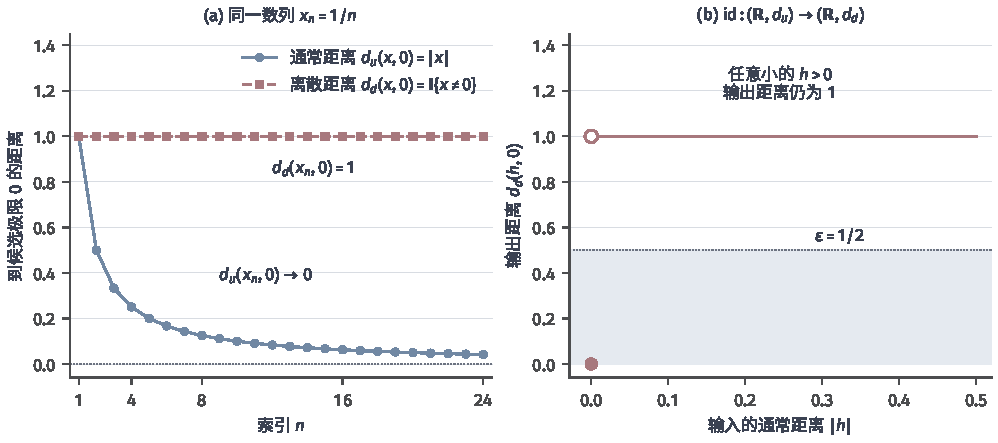
\includegraphics[width=169.0mm]{figures/01-mathematical-preliminaries-upper/01-mathematical-language-combinatorics-analysis-optimization/matplotlib/analysis-metric-convergence/figure.pdf}
 \caption{通常距离与离散距离给出不同的邻近关系，图中分别记为$d_u$和$d_d$。左图中$1/n$在通常距离下趋于$0$，在离散距离下与$0$的距离始终为$1$；右图比较恒等映射在两种距离之间的连续性。距离规则是度量空间结构的一部分。}
 \label{fig:analysis-metric-convergence}
\end{figure*}
若原集合已经给定距离，而只想取其中一部分观察，还需要说明子集怎样沿用原距离，这正是下一项的内容。

\subsubsection{子空间度量}
\label{sec:metric-subspace-metric}

将已有距离用于子集时，先确认限制规则仍然是度量，再用区间和球面说明它保留了什么、改变了什么。

\paragraph{子空间度量的定义}

只在原空间的一部分上观察点时，怎样保留原有的距离？
这里不重新规定两点的数值，而只把允许比较的点限制在子集内；
需要确认的是，缩小点的范围不会破坏度量公理。

\begin{definition}[子空间度量]
\label{def:metric-subspace}
设$(X,d)$为度量空间，$A\subseteq X$。定义
\[
  d_A=d\big|_{A\times A},\qquad d_A(x,y)=d(x,y)\quad(x,y\in A),
\]
则$(A,d_A)$也是度量空间，称为$(X,d)$的子空间，$d_A$称为\term{子空间度量}（subspace metric）。
\end{definition}

任取$A$中的两点或三点，它们同时也是$X$中的点，
所以非负性、零距离辨认、对称性和三角不等式都逐条从原空间继承；
$d_A$的值仍在$[0,\infty)$中，零距离辨认也没有因为限制点的范围而失效。
这一构造只改变允许选取的点，不改变已选两点之间的距离公式。

\paragraph{子空间度量的示例}

先取实轴中的区间$A=[0,1]$。对区间内的两点$s,t$，继承的距离仍是$|s-t|$。
端点$0,1$是否属于$A$只影响哪些点可以被选取，
不会为已经选定的两点另造距离数值；换成$(0,1)$时，内部任意两点的距离公式仍然相同。

再取欧氏空间中的球面$A=\{\bm{p}:\lVert\bm{p}\rVert_2=1\}$。
两点$\bm{p},\bm{q}$在子空间中的距离仍是环境欧氏距离$\lVert\bm{p}-\bm{q}\rVert_2$，
它等于连接两点的弦的长度，而不是沿球面行走的最短路径长度。
沿球面路径的最短长度需要用曲线长度另行定义，不能把这里继承的环境距离直接称为球面上的内蕴距离。
两个例子说明，限制到$A$以后真正改变的是球内允许出现的点：
同一个距离公式因此可能给出不同的相对邻域，下一节会把这一点写成子空间球与环境球的交集公式。

\subsection{伪距离与商度量}
\label{sec:metric-zero-distance-identification}

度量公理用零距离辨认不同对象。但有些观察规则只能看到对象的一部分特征，
天然允许不同原对象具有零距离。
本小节先放宽辨认条件，再讨论能否把不可区分的对象合并成一个新点，使合并后的类之间重新得到真正的距离。

\subsubsection{伪距离}
\label{sec:metric-pseudometric}

当观察规则忽略某些差异时，先检查剩余的距离公理是否还成立，再确定需要怎样辨认对象。

\paragraph{伪距离与不可区分对象}

从度量公理中只放宽“零距离必为同一点”这一条，其余要求全部保留，就得到伪距离。

\begin{definition}[伪距离]
\label{def:analysis-pseudometric}
设$X$为非空集合。函数$d:X\times X\to[0,\infty)$若对任意$x,y,z\in X$满足
\[
  d(x,x)=0,\qquad d(x,y)=d(y,x),\qquad d(x,z)\leq d(x,y)+d(y,z),
\]
就称为$X$上的\term{伪距离}（pseudometric，也称伪度量）。
它允许$x\neq y$时仍有$d(x,y)=0$。
\end{definition}

这里只是不再要求零距离蕴含$x=y$，并没有允许负距离，也没有破坏对称性或三角不等式。
例如在$\mathbb R^2$上令
\[
  d\bigl((x_1,x_2),(y_1,y_2)\bigr)=|x_1-y_1|.
\]
非负性、$d(x,x)=0$、对称性和三角不等式都直接来自绝对值；
但第一坐标相同、第二坐标不同的点，例如$(0,0)$与$(0,1)$，距离为零。
这个规则只记录第一坐标的差异，无法区分位于同一条竖直线上的点。

这个例子提出下一步的问题：若任务确实只区分被观察到的差异，
就应把零距离的对象归为同类，再问类与类之间的距离是否有唯一含义。
不能只凭“忽略差异”的直觉，就宣布商集上已经有了度量。

\subsubsection{零距离等价类与商度量}
\label{sec:metric-quotient-metric}

先用零距离建立等价类，再检查类之间的距离能否摆脱代表元的选择，最后把它与熟悉的例子对应起来。

\paragraph{零距离等价类}

在伪距离空间中定义
\[
  x\sim y\quad\Longleftrightarrow\quad d(x,y)=0.
\]
这一关系把被观察规则视为没有差异的对象归为同类。它确实是等价关系：
$d(x,x)=0$给出自反性，对称性给出$x\sim y\Rightarrow y\sim x$。
若$x\sim y$且$y\sim z$，则三角不等式给出
\[
  d(x,z)\leq d(x,y)+d(y,z)=0,
\]
而距离非负，故$d(x,z)=0$，即$x\sim z$，传递性成立。
记$x$所在的等价类为$[x]$，所有等价类组成商集$X/{\sim}$。

\paragraph{商度量的良定义与公理}

对两个等价类，自然想规定$\bar d([x],[y])=d(x,y)$。
但一个类里有许多代表元，必须先证明这个数值不随代表元改变。

\begin{definition}[商度量]
\label{def:metric-quotient}
在伪距离空间的商集$X/{\sim}$上定义
\begin{equation}
\label{eq:analysis-quotient-metric}
  \bar d([x],[y])=d(x,y).
\end{equation}
\end{definition}

设$x\sim u$、$y\sim v$，即$d(x,u)=d(v,y)=0$。沿新代表插入两段零距离，三角不等式给出
\[
  d(x,y)\leq d(x,u)+d(u,v)+d(v,y)=d(u,v).
\]
交换两组代表，又得到$d(u,v)\leq d(x,y)$，所以$d(x,y)=d(u,v)$，
式~\eqref{eq:analysis-quotient-metric}与代表元的选择无关，类之间的距离才有唯一含义。
非负性、对称性和三角不等式分别由原伪距离取等号或取不等式传到类上。
再由定义，
\[
  \bar d([x],[y])=0\ \Longleftrightarrow\ d(x,y)=0
  \ \Longleftrightarrow\ x\sim y\ \Longleftrightarrow\ [x]=[y],
\]
分离性被补回，所以$\bar d$是商集上的真正度量，$(X/{\sim},\bar d)$称为商度量空间。

回到只看第一坐标的例子：每个等价类
$[(a,b)]=\{(a,t):t\in\mathbb R\}$是一条竖直直线，
映射$[(a,b)]\mapsto a$把这些类一一对应到实轴，
类与类的距离就是第一坐标之差$|a-c|$。
被忽略的第二坐标并没有被恢复，而是不再作为比较对象出现。
后面的函数空间会把几乎处处相等的函数视为同一元素，
当前构造正说明了这种合并怎样消除零距离歧义；
具体的积分距离及其有限性条件，要在相应函数类上另行建立。

\section{集合的度量结构}
\label{sec:metric-set-structure}

本节固定一个度量空间$(X,d)$及其中的子集，研究集合中的点怎样分布、逼近与被覆盖。
邻域、开闭集和闭包描述一个点相对集合的位置；稠密与可分判断一个固定子集能在多大程度上代表全空间；
有界与全有界分别控制总体半径和任意精度下的覆盖数量；紧致性则进一步要求任意开覆盖都有有限子覆盖。
这些条件随后会用于判断连续映射的像与极值，以及点列能否在当前空间内取得极限。

\subsection{邻域、开闭集与闭包}
\label{sec:metric-local-set-relations}

本小节研究点与集合的邻近关系。邻域规定一个点附近的范围，开闭集把邻域判断施加于整个集合，
内部、闭包和边界描述点相对集合的位置。点到集合的距离在闭包的数值刻画中引入；
距离下确界是否由某一点达到，则留到后面紧致集上的映射应用中研究。

\subsubsection{邻域与相对邻域}
\label{sec:metric-neighborhoods}

先固定当前度量空间中的球与邻域，再缩小到子空间，说明同一个距离公式为何会产生不同的相对邻域。

\paragraph{开球与邻域}

如何用距离阈值精确表达“在一个点附近”？
给定中心点和正的半径，可以把所有足够接近中心的点收集成一个集合。

\begin{definition}[开球与邻域]
\label{def:metric-open-ball}
设$(X,d)$为度量空间，$x\in X$，$r>0$。集合
\[
  B(x,r)=\{y\in X:d(x,y)<r\}
\]
称为以$x$为中心、以$r$为半径的开球。
若集合$V\subseteq X$包含某个开球$B(x,r)$，即存在$r>0$使$B(x,r)\subseteq V$，就称$V$为$x$的一个邻域。
\end{definition}

开球的定义里要注意两点：不等式是严格的$d(x,y)<r$，半径$r$必须为正。
球的形状取决于度量：实轴上的球是开区间，欧氏平面上的球是圆盘，
离散空间中半径小于$1$的球只含中心一个点。
邻域只需包含某个开球，本身不必是开集，也不能因为含有$x$就自动成为$x$的邻域；
例如实轴上的闭区间$[0,1]$是其内点$1/2$的邻域，却不是端点$0$的邻域。
图~\ref{fig:analysis-ball-neighborhood}已在平面欧氏距离下把这两个对象分开画出。

开球中的每一点都带有一个完全落在该球内的小球。若$y\in B(x,r)$，令
\[
  \rho=r-d(x,y)>0,
\]
则对任意$z\in B(y,\rho)$，三角不等式给出
$d(x,z)\leq d(x,y)+d(y,z)<d(x,y)+\rho=r$，所以
\begin{equation}
\label{eq:metric-ball-is-open}
  B(y,\rho)\subseteq B(x,r).
\end{equation}
这一性质为下一项的开放性提供了局部理由，也提醒所有球都只在当前空间$X$中取点。

\paragraph{相对邻域}

同一个点在大空间和子空间中，为什么会有不同的邻域判断？
沿用\ref{sec:metric-subspace-metric}节的子空间度量可以直接比较两种球。

设$A\subseteq X$配备子空间度量$d_A$。为区分所在空间，把$A$中的球记为$B_A(x,r)$，把$X$中的球记为$B_X(x,r)$。由定义，
\begin{equation}
\label{eq:metric-relative-ball}
  B_A(x,r)=A\cap B_X(x,r)\qquad(x\in A,\ r>0),
\end{equation}
因为两边都恰好表示“属于$A$且与$x$的环境距离小于$r$”的点。距离数值没有改变，改变的是可取点的范围。

取$A=[0,1]\subseteq\mathbb R$和端点$0$。在子空间$A$中，$0$的一个小球是
\[
  B_A(0,r)=[0,r)\cap A,
\]
它包含$0$右侧一段属于$A$的点；但在实轴$\mathbb R$中，任何$B_{\mathbb R}(0,r)=(-r,r)$都含有负数，
因而$[0,r)\cap A$不可能包含任何围绕$0$的实轴球。
于是同一个集合是否为$0$的邻域，要附属于所在空间来回答。
对$x\in A$，$V\subseteq A$是$x$在$A$中的邻域，当且仅当它包含某个相对球$B_A(x,r)$。
这也预示开放与封闭同样要相对当前空间判断，不能把端点处的几何直觉直接当成一般定义。

\subsubsection{开集与闭集}
\label{sec:metric-open-and-closed}

把“点附近有一个球”的条件用于整个集合，就得到开集；对补集作同样检验，则得到闭集。

\paragraph{开闭集的邻域判据}

\begin{definition}[开集与闭集]
\label{def:metric-open-closed}
设$(X,d)$为度量空间，$U\subseteq X$。若对每个$x\in U$都存在$r>0$使$B(x,r)\subseteq U$，
就称$U$为开集。若补集$X\setminus U$是开集，就称$U$为闭集。
\end{definition}

定义中的半径允许随点改变：不同位置可以使用大小不同的球，只要求每个点各自拥有一个。
用实轴的开区间可以直接检验：每个内点都能取一个完全落在区间内的小球。
在离散空间中，任意子集都是开集，因为半径小于$1$的球只含中心，必然包含在该子集中；
其补集同样任意，所以离散空间的任意子集同时也是闭集。

把闭集的定义改写一次，更便于使用：$F$为闭集，当且仅当每个$x\notin F$都有一个球完全避开$F$。
这是因为$X\setminus F$为开集，恰好表示每个外点都被某个球包在补集内部。
这里先用补集关系解释闭性；闭集的序列判据要到点列语言建立后再证明，不用尚未建立的等价表述代替定义。

空集和全空间$X$既开又闭：空集没有需要检验的点，而每个$x\in X$都有包含于$X$的球，两者的补集也满足同样条件。
但不能由此认为所有集合非开即闭。在$\mathbb R$中，$[0,1)$不是开集，因为$0$处没有完全落在集合内的小球；它也不是闭集，因为外点$1$无法用一个球避开$[0,1)$。
图~\ref{fig:analysis-open-closed-relative}用实轴区间和子空间中的端点检验了这种对环境的依赖。

由式~\eqref{eq:metric-ball-is-open}可知每个开球都是开集：球内任一点都有完全包含于该球的小球。
进一步，任意多个开集的并仍是开集，因为并集中每个点都已属于其中某个开集，可以沿用它的球；
有限多个开集的交仍是开集，因为可取各点在这些开集中所得半径的最小值。
“有限”不能改成“任意”，例如
\[
  \bigcap_{n\geq1}\Bigl(-\frac1n,\frac1n\Bigr)=\{0\},
\]
每个区间都是开集，其交集$\{0\}$却不是开集。

\subsubsection{内部、闭包与边界}
\label{sec:metric-interior-closure-boundary}

下面先用邻域描述点相对集合的位置，再把这些位置条件改写成数值距离判据，最后在区间和子空间中核对。

\paragraph{内部、闭包与边界的邻域判据}

设$A\subseteq X$。若存在$r>0$使$B(x,r)\subseteq A$，就称$x$为$A$的\term{内点}（interior point）；
全部内点组成$A$的内部，记作$A^\circ$。
按定义有$A^\circ\subseteq A$。若$B(x,r)\subseteq A$，则球内每一点$y$又可由式~\eqref{eq:metric-ball-is-open}取一个留在$B(x,r)$中的小球，因而$y$也是内点；
这说明整个$B(x,r)$都包含在$A^\circ$中，内部$A^\circ$是开集。
于是$A$为开集时每个$x\in A$都是内点，即$A^\circ=A$；反之，若$A=A^\circ$，由内部为开集得到$A$为开集。

闭包描述的是另一种位置：若每个正半径球都与$A$相交，就称$x$为$A$的闭包点，全部闭包点组成\term{闭包}（closure）$\overline A$，即
\[
  \overline A=\{x\in X:\forall r>0,\ B(x,r)\cap A\neq\varnothing\}.
\]
显然$A\subseteq\overline A$。与内点要求“存在一个球包含于集合”相比，闭包要求“每一个球都接触集合”，所以闭包点不必已经属于$A$。
闭包本身是闭集。事实上，若$x\notin\overline A$，则存在$r>0$使$B(x,r)\cap A=\varnothing$。
对任意$y\in B(x,r/2)$，$B(y,r/2)\subseteq B(x,r)$也避开$A$，故$y\notin\overline A$。
这说明补集$X\setminus\overline A$中每点都有一个球留在补集中，所以$X\setminus\overline A$为开集。

由此可以建立$A$为闭集与$A=\overline A$的等价关系。若$A$为闭集而$x\notin A$，外点$x$拥有避开$A$的球，故$x\notin\overline A$，得到$\overline A\subseteq A$；连同$A\subseteq\overline A$，有$A=\overline A$。
反过来，若$A=\overline A$，而闭包已经证明为闭集，所以$A$为闭集。
这个等价关系会在后面的距离判据与点列判据中反复使用。

边界点要求每个球同时碰到$A$和它的补集$X\setminus A$，全部边界点记作$\partial A$。按定义，
\[
  \partial A=\overline A\cap\overline{X\setminus A}.
\]
又因为$x\notin A^\circ$恰好表示每个球都碰到补集，所以$\overline{X\setminus A}=X\setminus A^\circ$，从而
\begin{equation}
\label{eq:metric-boundary-difference}
  \partial A=\overline A\setminus A^\circ.
\end{equation}
内部、闭包和边界因此都能用同一族球刻画，区别只在球是包含于集合、接触集合，还是同时接触两侧。

\paragraph{点到集合的距离}

“每个球都碰到$A$”是一种球条件，还可以换成数值判据。
对非空集合$A$定义点$x$到$A$的距离
\begin{equation}
\label{eq:metric-distance-to-set}
  d(x,A)=\inf_{a\in A}d(x,a).
\end{equation}
由于候选距离非负，且任取一个$a_0\in A$便有$d(x,A)\leq d(x,a_0)<\infty$，
所以这个下确界是有限的非负数。它具有两条与下确界相符的性质：
每个候选距离都不小于$d(x,A)$；对任意$\varepsilon>0$，又都能选到$a\in A$使
\begin{equation}
\label{eq:metric-infimum-approx}
  d(x,a)<d(x,A)+\varepsilon.
\end{equation}
这种近似性质并不要求某个点恰好达到下确界。为统一叙述，约定$d(x,\varnothing)=+\infty$。

点到集合的距离随点的移动满足 Lipschitz 型估计。对非空$A$和任意$x,y$，
\[
  d(x,a)\leq d(x,y)+d(y,a)\qquad(a\in A).
\]
对右侧候选取下确界，得到$d(x,A)\leq d(x,y)+d(y,A)$；交换$x,y$再得反向不等式，故
\begin{equation}
\label{eq:metric-set-distance-lipschitz}
  \bigl|d(x,A)-d(y,A)\bigr|\leq d(x,y).
\end{equation}
这个估计说明距离函数随点连续变化，后面会用于连续性和极值问题。

更重要的是，距离为零恰好刻画闭包。对非空$A$，
\begin{equation}
\label{eq:metric-zero-distance-closure}
  x\in\overline A\quad\Longleftrightarrow\quad d(x,A)=0.
\end{equation}
若$d(x,A)=0$，则由式~\eqref{eq:metric-infimum-approx}，对每个$r>0$都能选到$a\in A$使$d(x,a)<r$，即$B(x,r)\cap A\neq\varnothing$；
反过来，若每个球都与$A$相交，则$d(x,A)<r$对所有$r>0$成立，而距离非负，故$d(x,A)=0$。
当$A$为闭集时，再用$A=\overline A$得到
\[
  d(x,A)=0\quad\Longleftrightarrow\quad x\in A.
\]
这些数值结论都是由球定义推出的，并没有另换闭包的含义。

\paragraph{区间的内部、闭包与边界}

在实轴上计算$(0,1)$和$[0,1]$，可以看到内部与闭包分别回答什么问题。两者的内部都是$(0,1)$，闭包都是$[0,1]$，边界都是$\{0,1\}$。
对开区间的端点，任意小球都碰到区间和补集，所以端点属于边界和闭包，却不属于内部或原集合；固定一个内部点，则能取足够小的球完全留在区间内。

换到子空间时，所有球都要改用相对球，结论也随之改变。$[0,1]$在它自身中的内部是整个$[0,1]$，因为端点处的相对球不必包含负数；这与它在实轴中的内部$(0,1)$不同。
再回看开区间的端点：$d(0,(0,1))=0$说明可以任意逼近，却不表示下确界由区间内某点达到。最近点要求式~\eqref{eq:metric-distance-to-set}的下确界由$A$中的点真正达到，这是在距离数值之外新增的存在性条件，将在紧致集的极值应用中研究。

\subsection{稠密子集与可分空间}
\label{sec:metric-countable-approximation}

固定一个代表子集，先研究它能否逼近空间中的所有点，再增加代表数量可数的要求。

\paragraph{稠密子集的判据与构造}

\begin{definition}[稠密子集]
\label{def:metric-dense}
设$D\subseteq X$。若$\overline D=X$，就称$D$在$X$中\term{稠密}（dense）。
\end{definition}

由闭包的球判据，稠密性等价于：对每个$x\in X$和每个$\varepsilon>0$，都能选到$a\in D$使$d(x,a)<\varepsilon$。
度量空间和被逼近的整个$X$保持固定，所选代表$a$可以随位置$x$与精度$\varepsilon$改变，不要求用同一个点应付所有情形。

有理数集$\mathbb Q$在实轴上稠密。给定$x\in\mathbb R$和$\varepsilon>0$，先取正整数$m$使$1/m<\varepsilon$，再选整数$k$满足
\[
  \frac{k}{m}\leq x<\frac{k+1}{m}.
\]
于是$0\leq x-k/m<1/m<\varepsilon$，所以有理点$k/m$落在$B(x,\varepsilon)$中。
这个构造是实际选出代表，而不是只凭$\mathbb Q$含有无限多个点下判断；一般空间中也要在每个球里找到代表，集合无限本身并不推出稠密。

稠密并不意味着集合含有一个非空开球。考虑任意开区间$(\alpha,\beta)$，把其中点作为$x$、取小于半长的精度，上一构造先给出区间内的有理点$q$。
再取充分大的正整数$n$使$\sqrt2/n<\beta-q$，则$q+\sqrt2/n$仍是区间中的无理数。
因此每个实轴小球既碰到$\mathbb Q$，也碰到它的补集，由内部、闭包和边界的判据得到
\[
  \mathbb Q^\circ=\varnothing,\qquad \overline{\mathbb Q}=\mathbb R,\qquad \partial\mathbb Q=\mathbb R.
\]
点可以任意接近$D$，与$D$是否包含一小片完整邻域，是两种不同的性质。

\paragraph{可分空间与可数代表}

在稠密性上再增加代表集可数的要求，就得到可分性。

\begin{definition}[可分空间]
\label{def:metric-separable}
若度量空间$X$存在一个可数的稠密子集$D$，就称$X$\term{可分}（separable）。
\end{definition}

这里要求同一套可数代表同时服务所有位置与精度，不能每次另换一套集合；
但对每个具体精度，仍可以使用$D$中不同的点，定义并不要求只靠有限多个代表。
若$X$本身可数，取$D=X$便说明$X$可分；但反方向不成立，因为不可数的$\mathbb R$具有可数稠密集$\mathbb Q$。
这里区分的是全部点的数量与代表点的数量，而不是两种不同的稠密定义。

不可数离散空间给出反例。在离散度量下，半径小于$1$的球都只含中心一个点；
稠密集必须碰到每个这样的单点球，因而只能等于整个不可数空间。所以不可数离散空间不可分。
与通常度量下的实轴对照可见，可分性取决于当前距离决定的邻近关系，而不只取决于底层集合的大小。

可分性允许一套可数代表应对所有精度。若换一种更强的条件，使每个精度都只需有限多个代表，
就能把各精度的有限代表取可数并，构造出这样一套可数稠密集。下面据此研究有限覆盖的要求。
还要注意，集合能被代表点逼近，并没有说明任意点列都能取得空间内的极限，后一个保证属于\ref{sec:metric-completeness}节。

\subsection{有界集与有限覆盖}
\label{sec:metric-covering-budgets}

本节固定集合及其子空间度量，先问能否用一个有限半径的球容纳整个集合，
再问每个指定精度下能否只用有限多个小球覆盖。
前者控制总体半径，后者控制任意小尺度下的代表数量；
把各精度的有限代表汇合，还能建立全有界与可分性之间的联系。

\subsubsection{有界集}
\label{sec:metric-boundedness}

从“一个有限半径的球能否容纳全体点”进入有界性，再用直径刻画同一要求。

\paragraph{有界性与直径}

\begin{definition}[有界集与直径]
\label{def:metric-bounded}
设$(X,d)$为度量空间，$A\subseteq X$。若存在中心$x_0\in X$和有限半径$R>0$使$A\subseteq B(x_0,R)$，就称$A$为\term{有界集}（bounded set）；空集按约定有界。
对非空$A$，定义直径
\[
  \operatorname{diam}A=\sup\{d(x,y):x,y\in A\},
\]
允许上确界为$+\infty$，$\operatorname{diam}A$读作集合的\term{直径}（diameter）；并约定$\operatorname{diam}\varnothing=0$。
\end{definition}

定义中中心是否取在$A$内不影响判断。若$A\subseteq B(x_0,R)$，任取固定点$a_0\in A$，由三角不等式
\[
  d(x,a_0)\leq d(x,x_0)+d(x_0,a_0)<2R\qquad(x\in A),
\]
换到以$a_0$为中心只需增大半径。

有界性与直径有限等价。若$A\subseteq B(x_0,R)$，则任意两点满足$d(x,y)<2R$，所以$\operatorname{diam}A\leq2R$。
反过来，若直径$D=\operatorname{diam}A<\infty$，固定$a_0\in A$，则$d(x,a_0)\leq D$对所有$x\in A$成立，
取任意半径$D+\varepsilon$（$\varepsilon>0$）便得到容纳$A$的开球。
对空集的两项约定也彼此相容。

实轴上的有限区间有界，全实轴无界。更有启发性的反例是无限离散空间：
任意不同点的距离都是$1$，所以整个空间包含在任一半径大于$1$的球中，仍然有界。
这说明有界只控制总体半径，并未保证在更小精度下只需有限多个代表点。

\subsubsection{全有界与有限$\varepsilon$网}
\label{sec:metric-total-boundedness}

先建立每个精度下的有限网要求，再说明它比有界更强，最后把一系列有限网汇成可数稠密集。

\paragraph{全有界与有限网}

\begin{definition}[全有界与有限$\varepsilon$网]
\label{def:metric-totally-bounded}
设$A$配备子空间度量。若对每个$\varepsilon>0$，都存在有限个中心$a_1,\ldots,a_N\in A$，使
\[
  A\subseteq\bigcup_{i=1}^{N}B_A(a_i,\varepsilon),
\]
就称$A$\term{全有界}（totally bounded），并称$\{a_1,\ldots,a_N\}$为$A$的一个\term{有限网}（finite net）。
\end{definition}

精度改变时可以重新选择有限网，定义并不要求一套固定的有限网同时控制所有精度；
但对每一个固定精度，代表的数量必须有限。

全有界推出有界。固定一个精度，例如$\varepsilon=1$，并取有限网$a_1,\ldots,a_N$。
令$M=\max_i d(a_1,a_i)$。每个$x\in A$都属于某个$B_A(a_i,1)$，于是
\[
  d(x,a_1)\leq d(x,a_i)+d(a_i,a_1)<1+M,
\]
所以整个$A$包含在以$a_1$为中心的有限半径球内。空集可用空覆盖处理，不必强选中心。

有界却不一定全有界。无限离散空间虽有界，但取$\varepsilon<1$时每个球只含中心一个点，
覆盖整个空间需要无限多个中心。
再看实轴上的有界区间：把区间分成有限个长度小于$\varepsilon$的小段，
从每个与区间相交的小段中选一个区间内的点，则同一段中任意两点距离小于$\varepsilon$，
这些选点构成有限$\varepsilon$网。论证对未封闭区间同样成立，网点不必选在被排除的端点上。

\paragraph{由有限网构造可数稠密集}

每个精度的有限覆盖，怎样汇成一套能逼近所有点的可数代表？

设$A$全有界。对每个$n\geq1$选取一个有限$2^{-n}$网$F_n$，并令
\[
  D=\bigcup_{n\geq1}F_n.
\]
每个$F_n$都是有限集，可数个有限集的并仍可数，所以$D$是可数集；
合并后得到的是一套固定代表集，但它一般不再有限。

给定$x\in A$和$\varepsilon>0$，先选$n$使$2^{-n}<\varepsilon$，再由$F_n$的覆盖性选$a\in F_n$满足
$d(x,a)<2^{-n}<\varepsilon$。由于$F_n\subseteq D$，每个$B(x,\varepsilon)$都碰到$D$，所以$D$在$A$中稠密。
因此全有界空间可分。

反方向不成立：通常度量下的$\mathbb R$可分，却不是有界的，而全有界已经推出有界，故$\mathbb R$不全有界。
此后若另一个条件保证每个精度都存在有限球覆盖，就可以直接使用上述构造得到可数稠密集。

\subsection{紧致集与有限子覆盖}
\label{sec:metric-compact-control}

把“每个精度重选有限球”的要求，与“从任意既定开覆盖中选有限成员”的要求比较，就得到紧致性。

\paragraph{紧致性的开覆盖定义}

\begin{definition}[开覆盖、有限子覆盖与紧致性]
\label{def:metric-compactness}
设$K$为度量空间$X$的子集，并把$K$自身作为配备继承距离的度量空间。
若一族在$K$中相对开的集合$\{U_\alpha\}_{\alpha\in I}$满足
\[
  K\subseteq\bigcup_{\alpha\in I}U_\alpha,
\]
就称这族集合为$K$的相对开覆盖；若其中有限多个成员的并仍包含$K$，就称它们构成有限子覆盖。
若$K$的每个开覆盖都有有限子覆盖，就称$K$紧致。
\end{definition}

有限子覆盖只能从原有覆盖成员中选取，不能另换一组集合；开覆盖本身可以含有无限多个成员。
空集由空子覆盖满足条件，按约定紧致。

\paragraph{紧致集的有限网与闭性}

固定$\varepsilon>0$，全部相对球$\{B_K(a,\varepsilon):a\in K\}$构成$K$的一个开覆盖。
若$K$紧致，就能从中选出有限个球覆盖$K$，它们的中心恰好给出一个有限$\varepsilon$网，所以紧致推出全有界。
再回用前面的两项构造：一次固定精度的覆盖控制总体半径，故紧集有界；
各精度有限网的可数并提供可数稠密集，故紧集可分。

紧集在环境空间中还是闭集。设$K$非空紧致，$x\in X\setminus K$。对每个$a\in K$令
\[
  r_a=\frac{d(x,a)}{3}>0,
\]
则相对集合$K\cap B_X(a,r_a)$覆盖$K$。由紧致性，可选出有限个中心$a_1,\ldots,a_N$，使这些相对球覆盖$K$。令
\[
  r=\min_{1\leq i\leq N}r_{a_i}>0.
\]
对$y\in B_X(x,r)$和每个$i$，三角不等式给出
\[
  d(y,a_i)\geq d(x,a_i)-d(x,y)>d(x,a_i)-r\geq d(x,a_i)-r_{a_i}=2r_{a_i}>r_{a_i},
\]
所以$B_X(x,r)$避开每个$B_X(a_i,r_{a_i})$，也避开被它们覆盖的$K$。
每个外点都有这样一个球，说明$X\setminus K$为开集，故$K$为闭集；
$K$为空时其补集为$X$，同样为闭集。

\paragraph{有界与全有界不保证紧致}

在一般度量空间中，闭且有界不足以推出紧致。
无限离散空间的整个空间既闭又有界，但由全部单点开集构成的开覆盖没有有限子覆盖，
因为每个单点开集只能覆盖一个点。这里有限半径不能限制小尺度覆盖所需的数量，与全有界失败的原因相同。

全有界也仍不够。通常度量下$K=(0,1)$已由有限个小段覆盖证明为全有界。考虑
\[
  U_n=\Bigl(\frac1n,1\Bigr),\qquad n\geq2.
\]
每个$U_n$在$K$中相对开；对任意$x\in K$，选$n>1/x$便有$x\in U_n$，所以$\{U_n\}_{n\geq2}$覆盖$K$。
但任取有限多个成员后，设$N$是其中最大的指标，它们的并仍只是$U_N$，遗漏了$1/(2N)\in K$。
故$K$不紧致，由全有界推出的可分性也不能代替紧致。

这个覆盖失败与点列缺少怎样的极限点有关。
全有界还要增加什么极限保证才能得到紧致，欧氏空间中闭且有界为何足够，
都要在\ref{sec:metric-compactness-tests}节结合点列与完备性说明。
图~\ref{fig:analysis-process-finite-open-cover}已经把闭区间的有限覆盖与这里的开区间失败覆盖画在一起，可对照观察有限子覆盖遗漏的位置。

\section{映射的连续性与距离控制}
\label{sec:metric-map-error-transfer}

固定映射以后，输入误差怎样限制输出误差，输出又能保留多少输入差异？
本节从一个基点附近的函数极限与连续性出发，比较全域共用半径和比例上界两种控制；
再加入比例下界，研究像上逆映射的误差。
紧致定义域还会使连续像保持紧致、实值输出达到极值，并把各点的连续控制合成为统一控制。

\subsection{函数极限与连续性}
\label{sec:metric-map-limits}

先固定两个度量空间及它们之间的映射，研究输入接近一个基点时输出能否接近一个确定目标，
以及这个目标与基点处函数值之间是什么关系。

\paragraph{函数极限与唯一性}

固定度量空间$(X,d_X)$、$(Y,d_Y)$和映射$f:D\subseteq X\to Y$。
为使输入确实能够穿过其他点接近$a\in X$，要求每个$\delta>0$都存在$x\in D$满足$0<d_X(x,a)<\delta$；
这正是第~\ref{sec:analysis-function-limits}节已经引入的聚点条件，这里把$a$称为$D$的聚点。

\begin{definition}[函数极限]
\label{def:metric-function-limit}
设$a$是$D$的聚点。若对候选$L\in Y$，每个$\varepsilon>0$都存在$\delta>0$，使
\[
  x\in D,\quad 0<d_X(x,a)<\delta
  \quad\Longrightarrow\quad d_Y(f(x),L)<\varepsilon,
\]
就称$x\to a$时$f(x)$趋于$L$，记作$\lim_{x\to a}f(x)=L$。
\end{definition}

这里$a$可以不属于$D$，条件也不使用$f(a)$；穿孔限制$0<d_X(x,a)$把基点本身排除在外。
这个输出目标若存在就是唯一的。若不同的$L_1,L_2$都满足极限条件，令
$\eta=d_Y(L_1,L_2)/3>0$，分别按$\eta$取得输入半径，再取两者中较小的一个$\delta$。
聚点条件保证穿孔小球$B_D(a,\delta)\setminus\{a\}$中仍有合法输入$x$。于是
\[
  d_Y(L_1,L_2)
  \leq d_Y(L_1,f(x))+d_Y(f(x),L_2)<2\eta,
\]
而$d_Y(L_1,L_2)=3\eta$，矛盾。聚点条件负责排除“没有输入可检验”的空条件；
它并不保证极限一定存在，只保证一旦存在就不会有两个不同目标。

\paragraph{连续与函数值}

当$a\in D$时，可以把候选目标换成基点处的函数值。

\begin{definition}[连续]
\label{def:metric-continuity-at-point}
设$f:D\subseteq X\to Y$，$a\in D$。若对每个$\varepsilon>0$都存在$\delta>0$，使
\[
  x\in D,\quad d_X(x,a)<\delta
  \quad\Longrightarrow\quad d_Y(f(x),f(a))<\varepsilon,
\]
就称$f$在$a$连续。若$f$在$D$的每一点都连续，就称$f$连续。
\end{definition}

在$a$也是$D$的聚点时，连续性与函数极限的关系很直接。
连续条件限制到穿孔输入便得到极限等于$f(a)$；反过来，若$\lim_{x\to a}f(x)=f(a)$，
同一个半径已经控制所有穿孔输入，而$x=a$时输出误差为零，故$f$在$a$连续。
因此在聚点处，
\[
  f\text{ 在 }a\text{ 连续}\quad\Longleftrightarrow\quad\lim_{x\to a}f(x)=f(a).
\]
若穿孔极限存在却不等于$f(a)$，极限的唯一性也排除了连续的可能。

若$a$是$D$中的孤立点，即存在$r>0$使$B_X(a,r)\cap D=\{a\}$，
则在这个半径内只有基点自身需要检验，$f$自动在$a$连续。
但相应的穿孔小球中没有输入，无论指定哪个$L\in Y$，定义~\ref{def:metric-function-limit}的阈值式都会空泛成立；
所以孤立点处不按聚点定义使用函数极限，也不能由这种空条件断言唯一的输出目标。
连续性的定义仍然适用于这样的定义域点。

\subsection{一致连续与Lipschitz条件}
\label{sec:metric-uniform-continuity}

在一点连续时，控制输入误差的半径可以随基点变化。
下面固定$f:D\subseteq X\to Y$及两端度量，比较何时能够共用一个半径，
以及何时能够用输入距离的固定比例控制输出距离。

\paragraph{逐点连续与一致连续}

逐点连续允许对每个基点$a\in D$和每个$\varepsilon>0$分别选择$\delta(a,\varepsilon)>0$。
一致连续则把半径提到基点之前：

\begin{definition}[一致连续]
\label{def:metric-uniformly-continuous}
设$f:D\subseteq X\to Y$。若对每个$\varepsilon>0$都存在$\delta>0$，使任意$x,y\in D$满足
\[
  d_X(x,y)<\delta\quad\Longrightarrow\quad d_Y(f(x),f(y))<\varepsilon,
\]
就称$f$在$D$上一致连续。
\end{definition}

后者要求同一个输入容差同时服务全域的所有输入对，因此一致连续推出$f$在每个基点处连续；
反方向一般不成立。用通常绝对值距离下的$f(x)=x^2$检验这一区别。
在基点$a$附近，$|x-a|<1$时
\[
  |x^2-a^2|=|x+a|\,|x-a|\leq(2|a|+1)|x-a|,
\]
取$\delta=\min\{1,\varepsilon/(2|a|+1)\}$便得到逐点连续，但这个半径随$a$增大。
为说明全实轴上不一致连续，固定输出容差$\varepsilon_0=1$。任给$\delta>0$，取
\[
  x>\max\!\left\{1,\frac1\delta\right\},\qquad y=x+\frac1x.
\]
则$|x-y|=1/x<\delta$，而
\[
  |x^2-y^2|=(y-x)(x+y)=\frac1x\Bigl(2x+\frac1x\Bigr)=2+\frac1{x^2}>1,
\]
所以每个候选统一半径都会遇到失败的输入对。

\paragraph{Lipschitz控制与连续性条件的关系}

一种取得统一半径的办法，是要求输出距离始终不超过输入距离的固定倍数。

\begin{definition}[全局Lipschitz条件]
\label{def:metric-lipschitz}
设$f:D\subseteq X\to Y$。若存在有限常数$L\geq0$，使所有$x,y\in D$满足
\begin{equation}
\label{eq:metric-lipschitz}
  d_Y(f(x),f(y))\leq L\,d_X(x,y),
\end{equation}
就称$f$满足全局Lipschitz条件，$L$称为一个Lipschitz常数。
\end{definition}

当$L>0$时，给定$\varepsilon>0$取$\delta=\varepsilon/L$，便得到一致连续；
当$L=0$时，任意两输入的输出距离为零，输出相同，也一致连续。
因此比例上界是比共用半径更具体的控制方式。

若全域共用常数过强，还可以只要求每个基点附近存在自己的比例常数：
存在$r_a>0$与有限$L_a\geq0$，使所有$x,y\in D\cap B_X(a,r_a)$满足
$d_Y(f(x),f(y))\leq L_a d_X(x,y)$。这称为局部Lipschitz条件。
令其中一个输入为$a$，便得到$f$在$a$连续；但不同基点的常数未必能合成一个全域常数。

仍以平方函数为例。固定$a$和$r>0$，邻域内$|x+y|\leq2(|a|+r)$，所以
\[
  |x^2-y^2|\leq 2(|a|+r)|x-y|,
\]
它在实轴上局部Lipschitz；前面的全实轴反例又说明它并不一致连续。
若把同一函数限制到$[0,1]$，则$|x+y|\leq2$给出全局Lipschitz常数$2$及一致连续，
说明定义域的范围本身也是条件的一部分。

再用$[0,1]$上的$f(x)=\sqrt x$检验一致连续能否反推Lipschitz。对$x>y$，
\[
  |\sqrt x-\sqrt y|=\frac{x-y}{\sqrt x+\sqrt y}.
\]
由$\sqrt x+\sqrt y\geq\sqrt{x-y}$，交换$x,y$并处理相等情形后可得
\[
  |\sqrt x-\sqrt y|\leq\sqrt{|x-y|},
\]
取$\delta=\varepsilon^2$便能统一控制输出，所以根号函数一致连续。
另一方面，$0$的任意相对邻域都含充分小的正$x$，而
\[
  \frac{|\sqrt x-\sqrt0|}{|x-0|}=\frac1{\sqrt x}
\]
在每个这样的邻域中无界，故它在$0$处不局部Lipschitz，也不存在全域Lipschitz常数。

综合起来，实际蕴含关系是
\[
  \text{全局Lipschitz}\Longrightarrow\text{一致连续}\Longrightarrow\text{连续},
\]
全局Lipschitz也推出局部Lipschitz，局部Lipschitz推出逐点连续；
但一致连续与局部Lipschitz之间没有一般蕴含关系：
$[0,1]$上的根号函数排除了“一致连续推出局部Lipschitz”，
全实轴上的平方函数排除了“局部Lipschitz推出一致连续”。
这些判断都针对已经固定的函数、定义域和两端度量，不能在改变范围后沿用同一结论。
第~\ref{chap:univariate-calculus}章在一元实函数情形还会引入绝对连续，
它控制许多小区间上的总增量，与这里的两个条件不是同一种要求。

\subsection{等距与双Lipschitz映射}
\label{sec:metric-isometry-bilipschitz}

式~\eqref{eq:metric-lipschitz}的比例上界仍允许不同输入落到同一输出：
常值映射满足Lipschitz上界，却无法从输出辨认输入。
若还要求输出距离至少保留输入距离的一个固定正比例，就需要加入下界，
它同时给出像上逆映射的Lipschitz误差控制。

\begin{definition}[等距映射与双Lipschitz映射]
\label{def:metric-isometry-bilipschitz}
设$f:D\subseteq X\to Y$。若
\[
  d_Y(f(x),f(y))=d_X(x,y)\qquad(x,y\in D),
\]
就称$f$为\term{等距映射}（isometry）。若存在常数$0<c\leq C<\infty$，使所有$x,y\in D$满足
\begin{equation}
\label{eq:metric-bilipschitz}
  c\,d_X(x,y)\leq d_Y(f(x),f(y))\leq C\,d_X(x,y),
\end{equation}
就称$f$为\term{双Lipschitz映射}（bi-Lipschitz mapping）。
\end{definition}

若$f(x)=f(y)$，下界给出$c\,d_X(x,y)\leq0$，而$c>0$，故$d_X(x,y)=0$；
再用度量的分离性得到$x=y$，所以双Lipschitz映射（包括等距映射）是单射。
于是可以在像$f(D)$上定义逆映射$f^{-1}$。对像内的$u=f(x)$、$v=f(y)$，重排下界得到
\begin{equation}
\label{eq:metric-inverse-lipschitz}
  d_X\bigl(f^{-1}(u),f^{-1}(v)\bigr)\leq\frac1c\,d_Y(u,v).
\end{equation}
这说明输出误差如何限制可恢复输入的误差；等距映射正是两侧常数都为$1$的特例。
逆映射的定义域始终是配备子空间度量的$f(D)$；在没有满射到整个$Y$的条件时，不能把它替换成整个$Y$。

实轴上的正比例缩放$f(t)=st$（$s>0$）满足式~\eqref{eq:metric-bilipschitz}，两侧常数都是$s$。
包含映射$j:(0,1)\to\mathbb R$，$j(t)=t$，则是等距映射，但它的像只是$(0,1)$，没有覆盖整个陪域。
两个例子分别检查距离比例与映射范围：不能仅凭等距，就把定义域的性质推广到整个陪域。
点列的收敛与柯西条件建立以后，还会把同一两侧距离界用于点列，
检验误差能否正反传递以及极限是否留在像中。

\subsection{紧致定义域上的连续映射}
\label{sec:metric-compactness-consequences}

固定紧致集合$K$及连续映射$f:K\to Y$。
本节先判断连续像是否紧致、实值输出能否达到极值，再把各点的连续半径合成一个统一半径。
极值路线利用像的闭性和实数的确界，最近点则把这一路线用于距离函数最小化；
一致连续路线利用有限球覆盖合并各点的误差控制。

\subsubsection{连续像与极值}
\label{sec:metric-continuous-images-extrema}

先证明连续像保持紧致，再讨论实值函数的最大值、最小值以及最近点的存在与非唯一。

\paragraph{连续像的紧致性}

设$K$紧致、$f:K\to Y$连续。要证明像$f(K)$紧致，先看$f$怎样把像中的相对开集拉回定义域。
设$U$是$f(K)$中的相对开集，且$f(x)\in U$。存在$r>0$使
\[
  B_Y(f(x),r)\cap f(K)\subseteq U.
\]
由$f$在$x$连续，可取$K$中的输入球，使其中点的输出都落入$B_Y(f(x),r)$；这些输出本就属于$f(K)$，因此仍属于$U$。这说明原像$f^{-1}(U)$在$K$中相对开。

现在任取$f(K)$的一个相对开覆盖$\{U_\alpha\}$。由上一步，$\{f^{-1}(U_\alpha)\}$是$K$的开覆盖；
$K$紧致，故有有限子覆盖$f^{-1}(U_{\alpha_1}),\ldots,f^{-1}(U_{\alpha_N})$。
对应的$U_{\alpha_1},\ldots,U_{\alpha_N}$覆盖$f(K)$，所以$f(K)$紧致。
证明不要求$f$单射，也不要求像覆盖整个$Y$。

\paragraph{实值函数的极值}

\begin{theorem}[紧集上实值连续函数的极值]
\label{thm:metric-extreme-value}
设$K$非空紧致，$f:K\to\mathbb R$连续，并使用实轴通常距离。则$f(K)$是$\mathbb R$中的非空紧集，
$f$在$K$上达到最大值和最小值。
\end{theorem}

\begin{proof}
由连续像的紧致性，$f(K)$紧致，而紧集在度量空间中闭且有界，所以$f(K)$是有界闭集。
令$M=\sup f(K)$。对任意$\varepsilon>0$，上确界近似给出$f(K)$中的值与$M$的距离小于$\varepsilon$，
故$M\in\overline{f(K)}$。由$f(K)$为闭集，$M\in f(K)$，即存在$x_*\in K$使$f(x_*)=M$，最大值达到。
对$-f$作同样论证得到最小值。
\end{proof}

这个定理不自动给出求解算法，也不保证达到极值的点唯一；它只保证下确界或上确界被实际取得。
条件缺失时结论可能失败：$f:(0,1)\to\mathbb R$，$f(t)=t$连续且值域有界，
却没有最大值和最小值，这里失去的是定义域的紧致性。

\paragraph{最近点的存在与非唯一性}

把紧集上连续函数的极值结论用于已经定义的点到集合距离，就得到最近点问题。
固定$x\in X$与非空$A\subseteq X$，最近点是满足
\[
  d(x,a_*)=d(x,A)
\]
的点$a_*\in A$。闭包的零距离判据说明$d(x,A)=0$时，$A$中的点可以任意接近$x$；
最近点则进一步要求定义距离时的下确界由允许集合中的某一点真正达到。

这两件事必须分开。取$A=(0,1)$：当$x=0$时$d(x,A)=0$，当$x=2$时$d(x,A)=1$，
但两种情形都没有$A$中的点达到相应下确界。距离值是否为零，与下确界是否达到，回答的是不同问题。

若$A$非空紧致，固定$x$。由式~\eqref{eq:metric-set-distance-lipschitz}，函数$a\mapsto d(x,a)$连续；
定理~\ref{thm:metric-extreme-value}保证它在$A$上取得最小值，
即存在$a_*\in A$使$d(x,a_*)=d(x,A)$，这就是所求最近点。
紧致性在这里保证存在性，不保证唯一性。例如$A=\{-1,1\}$、$x=0$时，两个点到$0$的距离都是$1$，最近点有两个。
唯一投影还需要线性结构、凸性及相应空间条件，留到函数空间中的投影问题讨论。

\subsubsection{紧集上的一致连续}
\label{sec:metric-compact-uniform-continuity}

在紧致定义域上，各点自己的连续控制可以合成为一个统一半径。

\begin{theorem}[Heine--Cantor定理]
\label{thm:metric-heine-cantor}
设$K$紧致，$f:K\to Y$连续，则$f$在$K$上一致连续。
\end{theorem}

\begin{proof}
$K$为空时结论按量词直接成立。设$K$非空，固定输出容差$\varepsilon>0$。
对每个$x\in K$，由连续性选择$r_x>0$，使$z\in K$且$d_X(x,z)<2r_x$时
\[
  d_Y(f(x),f(z))<\frac{\varepsilon}{2}.
\]
半径中预留的一倍余量，用于比较同一个小球内的两个点。
相对球族$\{B_K(x,r_x):x\in K\}$覆盖$K$；由紧致性取有限子覆盖
$B_K(x_1,r_1),\ldots,B_K(x_N,r_N)$，并令
\[
  \delta=\min_{1\leq i\leq N}r_i>0.
\]
任取$u,v\in K$且$d_X(u,v)<\delta$。先选$i$使$u\in B_K(x_i,r_i)$，即$d_X(u,x_i)<r_i$。三角不等式给出
\[
  d_X(v,x_i)\leq d_X(v,u)+d_X(u,x_i)<\delta+r_i\leq2r_i,
\]
所以两项输出都距$f(x_i)$小于$\varepsilon/2$。再用一次三角不等式，
\[
  d_Y(f(u),f(v))
  \leq d_Y(f(u),f(x_i))+d_Y(f(x_i),f(v))<\varepsilon.
\]
统一半径来自有限个正半径的最小值，而不是对所有点的半径取下确界；后者可能为零。
\end{proof}

回到平方函数在紧区间与全实轴上的对照：紧致是本定理的充分条件，
不能从全实轴平方函数这一非紧反例断言所有非紧定义域上的连续函数都不一致连续。
例如定义域非紧时，常值函数仍满足一致连续的量词。

\section{点列的收敛与生成}
\label{sec:metric-sequence-limits}

本节以点列为直接分析对象。先检验一列是否趋向给定的点，再研究空间在什么条件下保有整列或子列的极限，
然后把这些工具用于按自映射规则生成的迭代列。
完备与紧致分别承担相应的极限保证，误差估计则说明怎样把收敛结论变成可以检查的精度要求。

\subsection{点列的收敛与序列判据}
\label{sec:metric-convergent-sequences}

先建立收敛、子列和极限唯一性，再用点列刻画此前已经定义的闭包、闭性与映射连续性。
这些判据把点列的极限与前面的集合、映射条件联系起来。

\subsubsection{收敛与极限唯一性}
\label{sec:metric-convergence-and-uniqueness}

点列趋向一个指定点时，尾部需要满足怎样的距离条件？
先固定极限说明收敛及唯一性，再检查取值范围与子列的变化。

\paragraph{收敛与极限唯一性}

\begin{definition}[点列收敛]
\label{def:metric-convergence}
设$(x_n)$是度量空间$(X,d)$中的点列，$x\in X$。若对每个$\varepsilon>0$都存在$N$，使所有$n\geq N$满足
\[
  d(x_n,x)<\varepsilon,
\]
就称$(x_n)$收敛到$x$，记作$x_n\to x$，并称$x$为该点列的极限。
\end{definition}

这与第~\ref{sec:analysis-continuous-limits}节实数列的定义结构相同，只是把$|a_n-a|$换成一般距离$d(x_n,x)$；
要求约束的是整个尾部，而不是只出现无穷多次的项。
$1/n\to0$时整个尾部都进入以$0$为中心的任意小球。
交替列$(-1)^n$则不同：它有无穷多个项等于$1$，但奇数项始终与$1$相距$2$，
不能使整个尾部都接近$1$，所以它不收敛到$1$。

度量空间中的极限若存在则唯一。若同一列同时趋于$x$与$y$，对任意$\varepsilon>0$，取足够大的$n$使
$d(x_n,x)<\varepsilon/2$且$d(x_n,y)<\varepsilon/2$。三角不等式给出
\[
  d(x,y)\leq d(x,x_n)+d(x_n,y)<\varepsilon.
\]
由于$\varepsilon$任意，而$d(x,y)$是固定的非负数，故$d(x,y)=0$，再由分离性得$x=y$。
在未取商的伪距离中，这最后一步只能得到$x$与$y$零距离，不能认定原对象相同；
这也是\ref{sec:metric-quotient-metric}节要先商化的原因之一。

\paragraph{收敛列的有界性}

收敛列的取值集合有界。若$x_n\to x$，取尾部落在$B(x,1)$内；
前有限项到$x$的距离只有有限多个，设其中最大值与$1$比较后取较大的数作为半径，
便可把整列容纳在同一个以$x$为中心的球中。
有界性只限制取值范围，并不反过来保证收敛，交替列就是有界而不收敛的例子。

\paragraph{子列的收敛}

改变观察指标也很有用。设$n_1<n_2<\cdots$是严格递增的正整数列，则$(x_{n_k})_{k\geq1}$称为$(x_n)$的子列。
由于$n_k\geq k$，原列给出的任一尾部阈值最终也适用于子列：
若$x_n\to x$，则对充分大的$k$有$n_k\geq N$，所以$d(x_{n_k},x)<\varepsilon$，即每条子列都趋于同一极限$x$。

但存在一条收敛子列并不保证整列收敛。交替列$(-1)^n$的偶数项子列趋于$1$、奇数项子列趋于$-1$，
整列却没有极限。这就留下后面的问题：空间具有什么条件，才能从任意点列中至少选到一条收敛子列？
\ref{sec:metric-compactness-tests}节将用紧致性回答它。

\subsubsection{闭包与闭集的序列判据}
\label{sec:metric-sequential-closedness}

点列语言建立以后，可以把闭包和闭性改写为“极限能否从集合内取得”。
先从集合内取得逼近列，再用极限的归属刻画闭性。

\paragraph{闭包的序列刻画}

对$A\subseteq X$，有
\begin{equation}
\label{eq:metric-sequential-closure}
  x\in\overline A
  \quad\Longleftrightarrow\quad
  \text{存在取值于 }A\text{ 的点列 }(a_n)\text{ 使 }a_n\to x.
\end{equation}
正向构造如下：若$x\in\overline A$，则每个$B(x,1/n)$都与$A$相交，逐个选取$a_n\in B(x,1/n)\cap A$，便有$d(a_n,x)<1/n$，所以$a_n\to x$。
反向利用收敛的尾部条件：若$a_n\to x$，则任意$B(x,r)$都包含充分靠后的$a_n$，故每个球都与$A$相交，即$x\in\overline A$。
当$x\in A$时，允许取常值列$a_n=x$；空集没有这样的点列。

\paragraph{闭集的序列判据}

由式~\eqref{eq:metric-sequential-closure}立即得到闭集的序列判据：
\begin{equation}
\label{eq:metric-sequential-closed}
  A\text{ 为闭集}
  \quad\Longleftrightarrow\quad
  \text{取值于 }A\text{ 的收敛点列，其极限仍属于 }A.
\end{equation}
若$A$闭而极限$x$落在补集中，补集内有一个避开$A$的球，收敛尾部却必须进入这个球，矛盾。
反之，若$A$不闭，则存在$x\in\overline A\setminus A$；由式~\eqref{eq:metric-sequential-closure}可取$a_n\in A$使$a_n\to x\notin A$，构成反例。

用$(0,1)$中的$1/n$（$n\geq2$）检验：它在环境$\mathbb R$中趋于$0$，而$0\notin(0,1)$，所以$(0,1)$不是$\mathbb R$中的闭集。
改把环境设为子空间$(0,1)$自身时，$0$不再是环境中的候选极限，不能沿用实轴中的闭性判断。
这里说明的是极限的归属，尚未声称每个内部相互接近的点列都有极限。

\subsubsection{映射下的点列收敛}
\label{sec:metric-map-sequence-tests}

现在以点列为检测对象，刻画前面已经定义的函数极限与连续性，并检查双向距离界怎样保持收敛。

\paragraph{函数极限的序列判据}

设$a$是$D$的聚点。$f(x)\to L$（$x\to a$）当且仅当：对$D\setminus\{a\}$中任意满足$x_n\to a$的点列，都有$f(x_n)\to L$。
正向直接使用函数极限给出的$\delta$：充分靠后的$x_n$满足$0<d_X(x_n,a)<\delta$，于是$d_Y(f(x_n),L)<\varepsilon$。
注意必须是任意输入列都满足输出结论，不是只找到一列。

反向用否定量词。若极限条件失效，则存在固定的$\varepsilon_0>0$，使对每个$n$都能选到$x_n\in D$满足
\[
  0<d_X(x_n,a)<\frac1n,\qquad d_Y(f(x_n),L)\geq\varepsilon_0.
\]
这列输入趋于$a$，输出却不趋于$L$，与序列检验的假设矛盾。
这种“逐个$1/n$邻域选点”的构造与实轴上函数极限序列判据的证明机制相同，只是距离换成两端度量。

\paragraph{连续性的序列判据}

在$a\in D$处，连续性同样有序列刻画：
\begin{equation}
\label{eq:metric-continuity-sequential}
  f\text{ 在 }a\text{ 连续}
  \quad\Longleftrightarrow\quad
  \bigl(x_n\in D,\ x_n\to a\bigr)\ \Longrightarrow\ f(x_n)\to f(a).
\end{equation}
正向直接代入阈值；反向若不连续，按$1/n$选择趋于$a$却维持固定输出偏差的输入列即可。
这里不需要穿孔限制，因为输入项允许等于$a$，而此时输出本来就等于$f(a)$。

\paragraph{双Lipschitz映射下的收敛}

对满足式~\eqref{eq:metric-bilipschitz}的双Lipschitz映射$f$，点列收敛可以在两侧相互传递：
\[
  x_n\to x\quad\Longleftrightarrow\quad f(x_n)\to f(x).
\]
由上界，$d_Y(f(x_n),f(x))\leq C\,d_X(x_n,x)$，故$x_n\to x$推出像点列收敛；
由下界，$d_X(x_n,x)\leq d_Y(f(x_n),f(x))/c$，故反方向也成立。
输出极限明确是像内的$f(x)$，不能替换成任意$Y$中的点；
映射的单射性与像上逆误差界已经在\ref{sec:metric-isometry-bilipschitz}节建立。

\subsection{柯西列与极限存在}
\label{sec:metric-completeness}

收敛定义需要先给出候选极限。本节改问：只知道点列内部相互接近时，当前空间是否一定保有极限？
先定义柯西列与完备性，再分别证明闭子集继承完备性、构造度量空间的完备化，
最后检查双向映射下这些点列条件如何传递。完备性是对空间中所有柯西列的要求，不是某一条点列的名称。

\subsubsection{柯西列与完备性}
\label{sec:metric-cauchy-completeness}

不预先知道极限位置时，怎样从点列内部的距离判断它是否应当有一个终点？
先建立列内部的接近条件及其范围后果，再判断当前空间是否保有所需极限。

\paragraph{柯西列及其有界性}

\begin{definition}[柯西列]
\label{def:metric-cauchy}
点列$(x_n)$若对每个$\varepsilon>0$都存在$N$，使所有$m,n\geq N$满足
\[
  d(x_m,x_n)<\varepsilon,
\]
就称为柯西列。
\end{definition}

与收敛定义相比，这里比较的是尾部的任意两项，不使用外部候选极限。
每个收敛列都是柯西列：若$x_n\to x$，取充分靠后的$m,n$使两项与$x$的距离都小于$\varepsilon/2$，则
\[
  d(x_m,x_n)\leq d(x_m,x)+d(x,x_n)<\varepsilon.
\]

柯西列有界：取$\varepsilon=1$，尾部全部落在以某个尾项$x_N$为中心的有限球$B(x_N,1)$内，
再把有限个首项并入一个半径更大的球即可。
但有界不保证柯西或收敛：实轴交替列$(-1)^n$有界，偶数项与奇数项的距离恒为$2$，不是柯西列。
这些逐级条件——有界、柯西、收敛——不能混为一谈。

\paragraph{完备性与极限缺失}

\begin{definition}[完备度量空间]
\label{def:analysis-complete-metric-space}
若度量空间$X$中的每个柯西列都收敛到$X$中的某一点，就称$X$\term{完备}（complete）。
\end{definition}

实数在通常距离下完备，这由第~\ref{sec:analysis-continuous-limits}节的柯西收敛准则给出；
有限维欧氏空间的完备性将在\ref{sec:metric-closed-bounded-limits}节用坐标论证。
有理数空间$\mathbb Q$在通常距离下不完备。由$\mathbb Q$在$\mathbb R$中稠密，对每个$n$可选$a_n\in\mathbb Q$使
\[
  |a_n-\sqrt2|<\frac1n.
\]
该列在实轴上趋于$\sqrt2$，因而是柯西列；若它在$\mathbb Q$内也有极限$q$，
则在实轴中同一列的极限唯一，迫使$q=\sqrt2\notin\mathbb Q$，矛盾。
所以这条柯西列在$\mathbb Q$中没有极限。
图~\ref{fig:vol1-add-cauchy-completeness}把这列有理近似的数值与误差分开画出：尾部互近说明它满足柯西要求，完备性还负责保证极限属于当前空间。
\begin{figure}[!htbp]
  \centering
  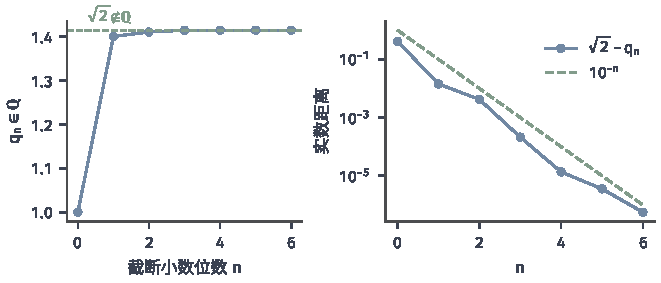
\includegraphics[width=112mm]{figures/01-mathematical-preliminaries-upper/01-mathematical-language-combinatorics-analysis-optimization/matplotlib/comprehension-additions/cauchy-completeness.pdf}
  \caption{由$\mathbb Q$在$\mathbb R$中稠密，对每个$n$选$a_n\in\mathbb Q$使$|a_n-\sqrt2|<1/n$。左图各项均为有理数，虚线是实数极限$\sqrt2$；右图的距离满足$0<\sqrt2-a_n<1/n$，用对数纵轴显示。有限个点不代替柯西性证明；该误差界与三角不等式才控制任意两个尾部项。}
  \label{fig:vol1-add-cauchy-completeness}
\end{figure}

再看$(0,1)$中的$1/n$（$n\geq2$）：它在环境实轴上趋于$0$，但$0$不在子空间中，
所以这列在$(0,1)$内缺少极限。两个例子共同说明，环境空间存在候选极限，并不保证子空间保有它。
稠密的$\mathbb Q$仍不完备，也区分了两件事：稠密描述对环境空间的任意精度逼近能力，完备描述对内部柯西列的极限保证。
接下来分别判断闭子集能否继承完备性，以及缺少极限的空间怎样扩充；
前面建立的双向距离界也可用来对应两侧柯西列，并据极限归属比较定义域与像的完备性。

\subsubsection{闭子集的完备性}
\label{sec:metric-closed-subspaces}

环境已经完备时，什么样的子集能够保留其中点列的极限？

\begin{theorem}[完备空间的闭子集完备]
\label{thm:metric-closed-subspace-complete}
设$X$完备，$A\subseteq X$为闭集，并配备子空间度量。则$A$完备。
\end{theorem}

\begin{proof}
任取$A$中的柯西列$(x_n)$。子空间度量与环境度量数值相同，所以它在$X$中仍是柯西列。
由$X$完备，存在$x\in X$使$x_n\to x$。再由闭集的序列判据~\eqref{eq:metric-sequential-closed}，$x\in A$。
于是该柯西列在$A$中收敛，$A$完备。
\end{proof}

环境完备负责“极限存在”，集合闭性负责“极限归属”，两步都不能省略。
空子集没有待检验的点列，按约定完备。
回看$(0,1)\subset\mathbb R$：环境完备，但子集没有保留趋于$0$的柯西列极限，这正是它不闭的后果。
若研究对象换成任意不完备空间，就不能只在原集合上宣布完备，而需要下一小节的扩张构造。

\subsubsection{度量空间的完备化}
\label{sec:metric-closed-subspaces-completion}

怎样用原空间的柯西列补入缺失的极限，并核对扩张后的空间确实完备？
先确定补入的点及点间距离，再把原空间安置进新空间，最后检验扩张空间能否保有任意柯西列的极限。

\paragraph{候选空间与度量}

先在度量空间$X$中收集全部柯西列，用它们表示可能缺失的极限候选。在柯西列之间定义
\[
  (x_n)\sim(y_n)\quad\Longleftrightarrow\quad d(x_n,y_n)\to0.
\]
自反性与对称性直接可得；若$(x_n)\sim(y_n)$、$(y_n)\sim(z_n)$，则
\[
  d(x_n,z_n)\leq d(x_n,y_n)+d(y_n,z_n)\to0,
\]
故传递性成立。以这些等价类组成候选空间
\[
  \widehat X=\bigl\{[(x_n)]:(x_n)\text{ 是 }X\text{ 中的柯西列}\bigr\}.
\]

接下来要为两个候选点规定距离。先固定两条柯西列$(x_n)$、$(y_n)$。反向三角不等式~\eqref{eq:metric-reverse-triangle}给出
\[
  \bigl|d(x_n,y_n)-d(x_m,y_m)\bigr|
  \leq d(x_n,x_m)+d(y_n,y_m).
\]
当$m,n$共同进入尾部时，右端任意小，所以实数列$\bigl(d(x_n,y_n)\bigr)$是柯西列；
由实数完备性，它有有限非负极限。于是可以定义
\begin{equation}
\label{eq:metric-completion-distance}
  D\bigl([(x_n)],[(y_n)]\bigr)=\lim_{n\to\infty}d(x_n,y_n).
\end{equation}

还要确认这个定义不依赖代表元。若$(x_n)\sim(u_n)$、$(y_n)\sim(v_n)$，则
\[
  \bigl|d(x_n,y_n)-d(u_n,v_n)\bigr|
  \leq d(x_n,u_n)+d(y_n,v_n)\to0,
\]
两个极限相等。对称性和三角不等式分别由原距离的相应性质取极限得到；而
\[
  D\bigl([(x_n)],[(y_n)]\bigr)=0
  \ \Longleftrightarrow\ d(x_n,y_n)\to0
  \ \Longleftrightarrow\ [(x_n)]=[(y_n)],
\]
分离性在类上恢复。因此$D$是$\widehat X$上的真正度量。

\paragraph{等距稠密嵌入}

把原空间的点映到常值列的等价类：令
\begin{equation}
\label{eq:metric-completion-embedding}
  i(x)=[(x,x,\ldots)].
\end{equation}
由式~\eqref{eq:metric-completion-distance}，
\[
  D(i(x),i(y))=\lim_{n\to\infty}d(x,y)=d(x,y),
\]
所以$i$保持距离，是\term{等距嵌入}（isometric embedding）；距离保持加上分离性使$i$单射。
后面始终保留映射$i$，不把原空间点与它的等价类暗中认成同一个对象。

原空间的像$i(X)$在$\widehat X$中稠密。固定新点$z=[(x_n)]$和$\varepsilon>0$。
因$(x_n)$是柯西列，存在$M$，使$m,n\geq M$时$d(x_m,x_n)<\varepsilon/2$。
固定任意$N\geq M$，对代表列的指标$n$取极限，得到
\[
  D(i(x_N),z)=\lim_{n\to\infty}d(x_N,x_n)\leq\frac{\varepsilon}{2}<\varepsilon.
\]
随着$N$增大，$i(x_N)$任意接近$z$，所以每个新点都在$i(X)$的闭包中。
这里“固定$N$、令$n$取极限”与“再让$N$增大”是两步不同操作，不能合并成一次取极限。

\paragraph{扩张空间的完备性}

\begin{theorem}[完备化]
\label{thm:metric-completion}
$\widehat X$是完备度量空间，且$i(X)$在$\widehat X$中稠密。
\end{theorem}

\begin{proof}
稠密性已经证明，只需证明$\widehat X$完备。任取$\widehat X$中的柯西列$(z_k)$。
由$i(X)$稠密，对每个$k$选原空间点$a_k\in X$，使
\[
  D(i(a_k),z_k)<2^{-k}.
\]
对任意$k,\ell$，等距性和三角不等式给出
\[
  d(a_k,a_\ell)=D(i(a_k),i(a_\ell))
  \leq 2^{-k}+D(z_k,z_\ell)+2^{-\ell}.
\]
当$k,\ell$共同进入尾部时，右端任意小，所以$(a_k)$是$X$中的柯西列。
这一步没有预先假定$z_k$已有极限。

令$z=[(a_k)]$，它是由上一柯西列给出的合法新点。把“等距稠密嵌入”中的常值类逼近用于代表列$(a_k)$，
有$D(i(a_k),z)\to0$。于是
\[
  D(z_k,z)\leq D(z_k,i(a_k))+D(i(a_k),z)<2^{-k}+D(i(a_k),z)\to0,
\]
即$z_k\to z$。每个$\widehat X$中的柯西列都有$\widehat X$内的极限，故$\widehat X$完备。
\end{proof}

构造至此给出等距稠密嵌入与\term{完备化}（completion）这一完备扩张；这里不额外声称已证明完备化在等距意义下唯一。

\subsubsection{双Lipschitz映射下的柯西列与完备性}
\label{sec:metric-map-cauchy-preservation}

双向距离界怎样对应两侧的柯西列，又怎样传递整个空间的完备性？
先对应两侧的列，再分别检查两个方向的极限落点。

\paragraph{柯西列的双向对应}

固定$f:D\subseteq X\to Y$满足式~\eqref{eq:metric-bilipschitz}。
上界使$D$中的柯西列映为像中的柯西列：若$(x_n)$柯西，则
\[
  d_Y(f(x_m),f(x_n))\leq C\,d_X(x_m,x_n)\to0.
\]
反过来，若像中的点列$y_n=f(x_n)$是柯西列，下界给出
\[
  d_X(x_m,x_n)\leq\frac1c\,d_Y(y_m,y_n)\to0,
\]
所以唯一的原像列也是柯西列；单射性保证“唯一原像”成立。

\paragraph{定义域与像的完备性}

在上述对应下，$D$与$f(D)$的完备性等价（像始终配备子空间度量）。

先设$D$完备。任取$f(D)$中的柯西列$y_n=f(x_n)$，由双向对应它的原像列$(x_n)$在$D$中柯西，
故$x_n\to x\in D$。再用上界，
\[
  d_Y(y_n,f(x))\leq C\,d_X(x_n,x)\to0,
\]
所以$y_n\to f(x)\in f(D)$，$f(D)$完备。这里是先拉回取极限，再用上界映出。

再设$f(D)$完备。任取$D$中的柯西列$(x_n)$，上界使$f(x_n)$成为像中的柯西列，
故它趋于某个$y\in f(D)$，可写$y=f(x)$且$x\in D$。下界给出
\[
  d_X(x_n,x)\leq\frac1c\,d_Y(f(x_n),f(x))\to0,
\]
所以$x_n\to x\in D$，$D$完备。
两个方向合起来得到$D$与$f(D)$完备性等价。
回看等距包含映射$j:(0,1)\to\mathbb R$：像$(0,1)$不完备而陪域$\mathbb R$完备，
因此只有满到整个陪域时，才能把像空间的结论表述为整个$Y$的结论。

\subsection{收敛子列与紧致性的序列刻画}
\label{sec:metric-compactness-tests}

现在任取点列，研究何时至少能得到一条在当前空间内收敛的子列。
本节回用集合节已经定义的紧致与全有界条件，证明紧致的序列刻画、
完备且全有界的联合判据，以及欧氏闭有界特例；这些等价证明把覆盖要求与极限保证连接起来。

\subsubsection{紧致与序列紧致}
\label{sec:metric-compact-sequential-tests}

此前的有限子覆盖条件，怎样等价于任意点列都能取到收敛子列？

若$K$中的每个点列都有一条收敛到$K$中某点的子列，就称$K$具有\term{序列紧致性}（sequential compactness）。
下面证明在度量空间中，紧致与序列紧致等价。
这是度量空间中的等价定理，不把结论外推到没有距离结构的任意拓扑空间。

\paragraph{紧致推出序列紧致}

先设$K$紧致，而$(x_n)$是$K$中的点列。
若不存在这样一个点，使它的每个邻域都含无穷多个序列指标，
则对每个$x\in K$都能取一个只含有限个指标的邻域$N_x$；
在其中选以$x$为中心的开球$U_x\subseteq N_x$，则$U_x$也只含有限个指标。
球族$\{U_x:x\in K\}$覆盖$K$，紧致性给出有限子覆盖$U_{x_1},\ldots,U_{x_N}$。
有限个“只含有限指标”的集合之并仍只含有限指标，与点列有无穷多个指标矛盾。

因此存在$x\in K$，使$x$的每个邻域都含无穷多个序列指标。
在$B(x,1/k)$中依次选取$n_k>n_{k-1}$，使$x_{n_k}\in B(x,1/k)$，便有$d(x_{n_k},x)<1/k$，
所以$x_{n_k}\to x$。这里计数的是序列指标；即使同一个取值重复出现，也能提供不同的指标。

\paragraph{序列紧致推出紧致}

再设$K$序列紧致，分两步推出开覆盖意义下的紧致。

第一步，序列紧致推出全有界。若某个$\varepsilon>0$没有有限个半径$\varepsilon$球覆盖$K$，
就可以递归选点：先选$x_1$，再从先前各点的$\varepsilon$球之外选$x_2$，如此继续，
使所得点列两两距离至少为$\varepsilon$。它的任何子列都不是柯西列，因而不可能收敛，与序列紧致矛盾。

第二步，证明对任意开覆盖$\mathcal U$，存在统一半径$r>0$，使每个$B(x,r)$都包含在某个覆盖成员中。
若不存在，对每个$n$选中心$x_n$，使$B(x_n,1/n)$不包含于任何$U\in\mathcal U$。
取收敛子列$x_{n_k}\to x$，并选$U_0\in\mathcal U$包含$x$；由$U_0$开，存在$R>0$使$B(x,R)\subseteq U_0$。
充分大的$k$同时满足$d(x_{n_k},x)<R/2$与$1/n_k<R/2$，三角不等式给出
\[
  B\!\left(x_{n_k},\frac1{n_k}\right)\subseteq B(x,R)\subseteq U_0,
\]
与$x_{n_k}$的选取方式矛盾，故统一半径$r$存在。

最后由全有界选有限个半径$r/2$的球覆盖$K$，设中心为$x_1,\ldots,x_N$。
每个$B(x_i,r)$都包含在某个原覆盖成员$U_i\in\mathcal U$中，
而$B(x_i,r/2)\subseteq B(x_i,r)\subseteq U_i$，所以$U_1,\ldots,U_N$覆盖$K$。
空空间的两种条件都直接成立。至此紧致与序列紧致等价。

\subsubsection{完备与全有界判据}
\label{sec:metric-complete-totally-bounded}

哪些空间条件能同时保证小尺度下不无限分散，并保住所构造子列的极限？

对空间$K$及其自身度量陈述结论：
\begin{theorem}[紧致的完备且全有界判据]
\label{thm:metric-complete-totally-bounded}
度量空间$K$紧致，当且仅当$K$完备且全有界。
\end{theorem}
若$K$是环境空间的子集，所有条件都按它的子空间度量解释，不能把环境的完备性直接移给$K$。

\paragraph{紧致空间的完备性}

集合节已经证明紧致推出全有界，只需再证紧致推出完备。
任取柯西列$(x_n)$。由紧致推出序列紧致，存在子列$(x_{n_k})$趋于某个$x\in K$。
给定$\varepsilon>0$，取$N$使$m,n\geq N$时$d(x_m,x_n)<\varepsilon/2$；
再取足够大的$k$，使$n_k\geq N$且$d(x_{n_k},x)<\varepsilon/2$。
于是对每个$n\geq N$，
\[
  d(x_n,x)\leq d(x_n,x_{n_k})+d(x_{n_k},x)<\varepsilon,
\]
所以整列收敛于$K$中的$x$，$K$完备。

\paragraph{完备且全有界空间的紧致性}

设$K$完备且全有界。对任意点列，逐层使用有限球覆盖：
第$j$层用有限个半径$2^{-j}$的球覆盖$K$，从上一层保留的无穷指标集中，
选出落入某个球的无穷子集。各层指标集逐层包含，但所选的球本身不必嵌套。

从第$j$层的指标集中选递增指标$n_j$，使$n_j$属于第$j$层选出的集合。
当$k,\ell\geq j$时，$x_{n_k}$与$x_{n_\ell}$都在第$j$层同一个半径$2^{-j}$的球中，
所以$d(x_{n_k},x_{n_\ell})<2^{1-j}$，子列$(x_{n_j})$是柯西列。
由完备性，它趋于某个$x\in K$；再由序列紧致与紧致的等价性，$K$紧致。

两个条件各负责一个不可省略的保证：$\mathbb R$完备却不全有界，$(0,1)$全有界却不完备。
可分性也不能代替全有界：可数无限离散空间可分（它本身可数）又有界，却不全有界，更不紧致。
另一方面，紧致空间由全有界及前面的有限网构造自动可分。因此有界与可分合起来，不能替代任意精度的有限覆盖。

\subsubsection{欧氏空间的闭有界判据}
\label{sec:metric-closed-bounded-limits}

利用点列与完备性，可以说明有限维欧氏空间的闭有界集为何紧致。
集合节已证明紧致在任意环境度量空间中都闭且有界，也给过无限离散空间的反例；
本小节只补欧氏空间的充分方向：对闭有界集分别取得完备性与全有界，再回用前一判据。

\paragraph{欧氏闭子集的完备性}

先证明$\mathbb R^d$完备。设$(\bm{x}_n)$是$\mathbb R^d$中的柯西列，记$\bm{x}_n=(x_{n,1},\ldots,x_{n,d})$。
由于
\[
  |x_{m,j}-x_{n,j}|\leq\lVert\bm{x}_m-\bm{x}_n\rVert_2,
\]
每个坐标列$(x_{n,j})_{n\geq1}$都是实数柯西列，由实数完备性有极限$x_j$。
令$\bm{x}=(x_1,\ldots,x_d)$。给定$\varepsilon>0$，让有限个坐标差同时小于$\varepsilon/\sqrt d$，则
\[
  \lVert\bm{x}_n-\bm{x}\rVert_2
  =\sqrt{\sum_{j=1}^{d}|x_{n,j}-x_j|^2}<\varepsilon,
\]
所以$\bm{x}_n\to\bm{x}$，$\mathbb R^d$完备。
由定理~\ref{thm:metric-closed-subspace-complete}，$\mathbb R^d$的闭子集配备子空间度量后也完备。

\paragraph{欧氏有界集的有限网}

再证明$\mathbb R^d$中的有界集全有界。设有界集$A$包含在一个有限边长的包围盒中。
对每个$\varepsilon>0$，用边长小于$\varepsilon/\sqrt d$的有限网格分割包围盒；
在每个与$A$相交的格子中选一个$A$内的点作为中心。
同一格子中任意两点的各坐标差都小于$\varepsilon/\sqrt d$，故欧氏距离小于$\varepsilon$，
这些有限个选点给出中心位于$A$中的有限$\varepsilon$网。
有限维性质在这里保证有限个坐标、有限个格子足以控制全体方向；空集可直接处理。

\paragraph{闭有界与紧致的等价}

把两条论证合并：闭性使$A$作为子空间完备，有界性使它全有界，
再由定理~\ref{thm:metric-complete-totally-bounded}，闭且有界的欧氏子集紧致。
与一般必要性合起来，得到有限维欧氏空间中的闭有界判据（Heine--Borel定理）：
\begin{equation}
\label{eq:metric-heine-borel}
  A\subseteq\mathbb R^d\text{ 紧致}\quad\Longleftrightarrow\quad A\text{ 闭且有界}.
\end{equation}

最后划定适用范围。在任意度量空间中，紧致都保证闭且有界；反向需要额外结构，
不能从欧氏特例直接外推，无限离散空间正说明闭且有界仍可缺少有限网。
一般判据始终是空间自身完备且全有界。

\subsection{压缩迭代的收敛与误差}
\label{sec:metric-contractive-solvers}

给定自映射$T:X\to X$，寻找满足$Tx_*=x_*$的点$x_*\in X$，称这样的点为$T$的不动点。
从起点$x^{(0)}$按
\[
  x^{(n+1)}=Tx^{(n)}
\]
生成候选点列以后，要研究它能否趋向这一目标，以及怎样控制误差。
迭代等式给出生成规则，压缩不等式则是保证点列收敛的条件。
在非空完备空间、自映射和统一压缩常数的共同条件下，先证明精确执行的结论，
再说明近似执行会增加哪些误差项。

\subsubsection{精确压缩迭代}
\label{sec:metric-exact-contraction}

本小节对同一迭代分别给出定性的不动点存在唯一性和定量的停止误差界。
这里建立的空间条件与误差估计，也将用于函数空间中求函数解的迭代。

\paragraph{不动点的存在与唯一}

对于目标方程$Tx_*=x_*$，什么条件能保证迭代$x^{(n+1)}=Tx^{(n)}$趋向唯一解？

\begin{definition}[不动点与压缩映射]
\label{def:analysis-fixed-point}
设$T:X\to X$为映射。点$x_*\in X$若满足$T(x_*)=x_*$，就称为$T$的\term{不动点}（fixed point）。
若存在$q\in[0,1)$，使所有$x,y\in X$满足
\begin{equation}
\label{eq:analysis-contraction-definition}
  d(Tx,Ty)\leq q\,d(x,y),
\end{equation}
就称$T$为\term{压缩映射}（contraction mapping），$q$称为压缩常数。
\end{definition}

压缩条件要求同一个严格小于$1$的常数在整个$X$上成立，并且$T$确实把$X$映回自身。

\begin{theorem}[Banach压缩映射定理]
\label{thm:analysis-banach-fixed-point}
设$(X,d)$是非空完备度量空间，$T:X\to X$是压缩常数为$q<1$的压缩映射。
则$T$有唯一不动点$x_*\in X$，并且从任意$x^{(0)}\in X$出发，由$x^{(n+1)}=Tx^{(n)}$生成的点列都收敛到$x_*$。
\end{theorem}

\begin{proof}
$q=0$时$T$为常值映射，一步即到不动点。以下设$0<q<1$。反复使用压缩条件，相邻两项满足
\[
  d\bigl(x^{(n+1)},x^{(n)}\bigr)
  \leq q\,d\bigl(x^{(n)},x^{(n-1)}\bigr)
  \leq q^n d\bigl(x^{(1)},x^{(0)}\bigr).
\]
对$m>n$，先用三角不等式串接相邻差，再求有限几何和：
\begin{align*}
  d(x^{(m)},x^{(n)})
  &\leq\sum_{j=n}^{m-1}d\bigl(x^{(j+1)},x^{(j)}\bigr)\\
  &\leq d\bigl(x^{(1)},x^{(0)}\bigr)\sum_{j=n}^{m-1}q^j\\
  &=\frac{q^n(1-q^{m-n})}{1-q}d\bigl(x^{(1)},x^{(0)}\bigr)
  \leq\frac{q^n}{1-q}d\bigl(x^{(1)},x^{(0)}\bigr).
\end{align*}
最后一个上界对所有$m>n$同时成立，并随$n$趋于零，所以迭代列是柯西列。
由完备性，存在$x_*\in X$使$x^{(n)}\to x_*$。压缩不等式~\eqref{eq:analysis-contraction-definition}还说明$T$连续，
因此$Tx^{(n)}\to Tx_*$；另一方面$Tx^{(n)}=x^{(n+1)}\to x_*$，
由极限唯一性得到$Tx_*=x_*$。这里先靠完备性取得候选极限，再靠映射的连续性验证它满足目标方程。

若$y_*$也是不动点，则
\[
  d(x_*,y_*)=d(Tx_*,Ty_*)\leq q\,d(x_*,y_*).
\]
由于$q<1$，只有$d(x_*,y_*)=0$，即$x_*=y_*$，不动点唯一。
\end{proof}

非空保证可以选择起点，自映射保证迭代能一直继续，完备性和严格压缩分别负责取得极限与收敛到不动点。
缺少条件时不能据此保证结论：在$(0,1)$上$T(x)=x/2$是严格压缩，但唯一可能的不动点$0$不在空间内；
在$\mathbb R$上$T(x)=x+1$只有Lipschitz常数$1$，它没有不动点。
这两个反例不是说缺少条件时所有问题都失败，而是说上述保证不再适用。

\paragraph{先验与后验误差界}

尚未知道不动点位置时，怎样从起点或已算相邻项估计当前误差？
记$e_n=d(x^{(n)},x_*)$。在证明中的尾和估计令$m\to\infty$，利用$x^{(m)}\to x_*$，得到先验界
\begin{equation}
\label{eq:analysis-banach-apriori-error}
  e_n\leq\frac{q^n}{1-q}d\bigl(x^{(1)},x^{(0)}\bigr).
\end{equation}
它只需要初始差和已知常数$q$，下标$n$从$0$开始计数。

从第$n$步起重新计算尾和，则得到后验界
\begin{equation}
\label{eq:analysis-banach-aposteriori-error}
  e_n\leq\frac{1}{1-q}d\bigl(x^{(n+1)},x^{(n)}\bigr).
\end{equation}
若只使用刚完成的两项且$n\geq1$，先用
$d(x^{(n+1)},x^{(n)})\leq q\,d(x^{(n)},x^{(n-1)})$控制尚未计算的下一步差，再代入上式，可得
\[
  e_n\leq\frac{q}{1-q}d\bigl(x^{(n)},x^{(n-1)}\bigr).
\]
两个式子对应不同数据条件：前者已知下一项，后者只知道当前项与前一项。

因此可以按目标误差$\varepsilon$，用式~\eqref{eq:analysis-banach-apriori-error}预先选择迭代步数，
也可以在每一步用式~\eqref{eq:analysis-banach-aposteriori-error}判断是否停止。
相邻差小只有结合收缩常数才成为误差证据：当$q$接近$1$时，因子$1/(1-q)$会放大上界，
不能只报告相邻差已经很小。

例如$T(x)=x/2+1$、$x^{(0)}=0$时，压缩常数$q=1/2$，$x^{(1)}=1$，唯一不动点是$2$。
先验界给出$|x^{(n)}-2|\leq2^{1-n}$，要求误差不超过$10^{-3}$时取$n=11$已足够；
后验界在这里化为$|x^{(n)}-2|\leq|x^{(n)}-x^{(n-1)}|$，无需事先知道答案$2$就能停止。
图~\ref{fig:vol1-add-contraction-cobweb}把这一迭代画成蛛网折线。
\begin{figure}[!htbp]
  \centering
  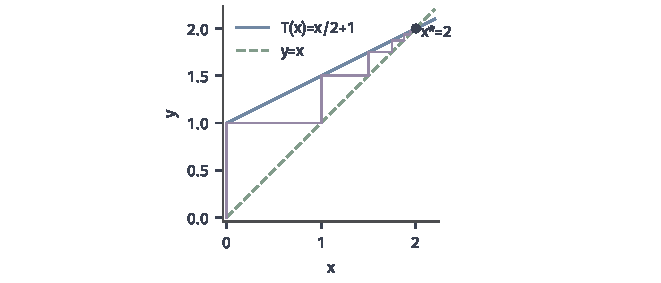
\includegraphics[width=112mm]{figures/01-mathematical-preliminaries-upper/01-mathematical-language-combinatorics-analysis-optimization/matplotlib/comprehension-additions/contraction-cobweb.pdf}
  \caption{$T(x)=x/2+1$在$[0,2]$上的七步迭代，初值$x^{(0)}=0$。蓝线是$T$，绿虚线是恒等函数，紫折线交替完成求值与复制；交点为$x_*=2$。精确迭代为$x^{(n)}=2-2^{1-n}$，图中的几何收缩对应压缩常数$1/2$。}
  \label{fig:vol1-add-contraction-cobweb}
\end{figure}

以上结论都假定精确执行$x^{(n+1)}=Tx^{(n)}$。若一次执行带有误差，
应把该误差单独写入递推再估计，不能直接照抄精确后验界；这就是下一小节的内容。

\subsubsection{带扰动的压缩迭代}
\label{sec:metric-perturbed-contraction}

每一步都只能近似执行压缩映射时，误差会消失还是累积到某个水平？
先跟踪每步执行误差的传播，再在不同扰动条件下估计极限行为，最后用已算数据认证当前精度。

\paragraph{扰动误差的递推与传播}

保持非空完备空间、自映射$T$与统一压缩常数$0\leq q<1$。
现在$x^{(n)}$表示近似执行得到的点列，每个计算点仍在$X$中，并满足
\begin{equation}
\label{eq:analysis-perturbed-execution}
  d\bigl(x^{(n+1)},Tx^{(n)}\bigr)\leq\eta^{(n)},\qquad \eta^{(n)}\geq0.
\end{equation}
以前项已证明存在唯一的精确不动点$x_*$为参照，令$e_n=d(x^{(n)},x_*)$。
由三角不等式和$Tx_*=x_*$，
\[
  e_{n+1}
  \leq d\bigl(x^{(n+1)},Tx^{(n)}\bigr)+d\bigl(Tx^{(n)},Tx_*\bigr)
  \leq \eta^{(n)}+q e_n,
\]
即
\begin{equation}
\label{eq:analysis-perturbed-distance-recursion}
  e_{n+1}\leq q e_n+\eta^{(n)}.
\end{equation}
% 保留内容迁移前的语义标签，指向同一公式。
\begingroup
\makeatletter
\let\label\ltx@label
\label{eq:prelim-perturbed-recurrence}
\endgroup
右边清楚区分了旧误差的收缩与本步新增误差。

先代入两步核对：
\[
  e_1\leq qe_0+\eta^{(0)},\qquad
  e_2\leq q^2e_0+q\eta^{(0)}+\eta^{(1)}.
\]
由同一递推归纳得到
\begin{equation}
\label{eq:analysis-perturbed-distance-unrolling}
  e_n\leq q^n e_0+\sum_{j=0}^{n-1}q^{\,n-1-j}\eta^{(j)}.
\end{equation}
% 保留内容迁移前的语义标签，指向同一公式。
\begingroup
\makeatletter
\let\label\ltx@label
\label{eq:prelim-unrolled-recurrence}
\endgroup
第$j$步加入的误差$\eta^{(j)}$经过此后$n-1-j$次收缩，因而带上相应幂次$q^{n-1-j}$。
前两步展开也可用来核对求和的起止下标与最新误差项的权重。

\paragraph{扰动误差的渐近估计}

若所有执行误差都有统一上界$\eta^{(j)}\leq\eta$，有限几何和给出
\[
  e_n\leq q^n e_0+\eta\frac{1-q^n}{1-q},
\qquad
  \limsup_{n\to\infty}e_n\leq\frac{\eta}{1-q}.
\]
这是误差的上界，不是实际误差的等式，也不是不可突破的下界；它不保证点列或误差列一定有极限。
当$q$接近$1$时，同样的执行误差对应更大的保证范围。

若$\eta^{(j)}\to0$，则$e_n\to0$。给定$\varepsilon>0$，先固定$J$，使$j\geq J$时
$\eta^{(j)}\leq(1-q)\varepsilon/2$。式~\eqref{eq:analysis-perturbed-distance-unrolling}的加权和中，
$j\geq J$的晚期部分由几何和控制在$\varepsilon/2$以内；$j<J$的早期部分只有有限项，
其权重随$n$衰减，连同$q^ne_0$在充分大的$n$时小于$\varepsilon/2$。
可求和误差是保证误差趋零的一项更强条件，它与“误差列趋零”并不互斥：趋零已经足够，可求和时估计通常更整齐。

\paragraph{带扰动的后验误差界}

还可以把已知执行误差转成可计算的停止界。由$Tx_*=x_*$与压缩条件，
\[
  e_n=d(x^{(n)},x_*)\leq d(x^{(n)},Tx^{(n)})+d(Tx^{(n)},Tx_*)\leq d(x^{(n)},Tx^{(n)})+q e_n,
\]
所以
\begin{equation}
\label{eq:metric-perturbed-residual-bound}
  e_n\leq\frac{1}{1-q}d(x^{(n)},Tx^{(n)}).
\end{equation}
若已算出$x^{(n+1)}$并有本步界$\eta^{(n)}$，则
$d(x^{(n)},Tx^{(n)})\leq d(x^{(n+1)},x^{(n)})+\eta^{(n)}$，代入得到
\begin{equation}
\label{eq:metric-perturbed-posterior-next}
  e_n\leq\frac{d(x^{(n+1)},x^{(n)})+\eta^{(n)}}{1-q},
\end{equation}
它认证的是点$x^{(n)}$。若要用刚完成的第$n-1$步直接认证$x^{(n)}$，则在$n\geq1$时把上一步界代入递推：
\[
  e_n\leq q\,e_{n-1}+\eta^{(n-1)}
  \leq\frac{q\,d(x^{(n)},x^{(n-1)})+\eta^{(n-1)}}{1-q}.
\]

\begin{example}[持续扰动与衰减扰动]
\label{ex:prelim-recurring-perturbations}
取$e_0=1$、$q=1/2$，并暂把递推中的不等号取为等号。若每步都加入$\eta^{(j)}=0.1$，则
\[
  e_n=2^{-n}+0.1\sum_{j=0}^{n-1}2^{-j}=0.2+0.8\cdot2^{-n},
\]
初始误差逐步消失，持续加入的误差却留下$0.2$的极限上界。若改为$\eta^{(j)}=0.1/(j+1)$，
扰动本身衰减，稳定递推使$e_n\to0$。例如第$1$步两者都是$0.6$，第$2$步分别为$0.4$和$0.35$；
差别来自第二步加入的新误差，而不是初值不同。
\end{example}
图~\ref{fig:prelim-perturbed-recurrence}比较了两种递推的轨迹。
\begin{figure}[htbp]
  \centering
  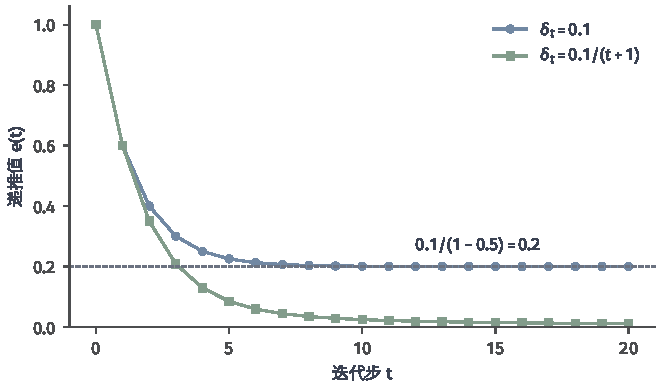
\includegraphics[width=112.0mm]{figures/01-mathematical-preliminaries-upper/01-mathematical-language-combinatorics-analysis-optimization/matplotlib/prelim-perturbed-recurrence/figure.pdf}
  \caption{相同初值与收缩系数下的两种递推。蓝线使用持续扰动，绿线使用衰减扰动；每个点都是整数步上的精确递推值，灰虚线是持续扰动留下的极限$0.2$。图为教学构造。}
 \label{fig:prelim-perturbed-recurrence}
\end{figure}

最后要核对停止结论依赖的资料：必须有同一个精确映射$T$、可用的统一常数$q$和相应执行误差界，
且近似点始终留在$X$中，才能把残差或相邻步长变成上述保证。
这里不把一般不稳定迭代或未知映射误差纳入已证明的压缩结论；
误差趋零的长期极限结论，与某一步达到指定精度的认证，也分别使用相应条件。

\section{本章小结}
\label{sec:metric-summary}

本章从度量规则进入集合、映射和点列。
集合侧用邻域与开闭集说明位置关系，用稠密子集说明任意精度的逼近，
再区分一套可数稠密代表与每个精度下的有限$\varepsilon$网。
全有界推出有界和可分，有界加可分仍不足以推出全有界；
紧致则以任意开覆盖都有有限子覆盖为正式定义，紧致集在环境空间中闭、有界、全有界且可分。

映射侧区分逐点连续、一致连续、Lipschitz与双Lipschitz所要求的距离控制。
连续映射把紧致定义域映成紧致像；定义域非空时，实值连续函数因而取得极值，
连续映射在紧集上还获得一致连续性。这些存在性与连续性结论本身不保证极值或最近点唯一，也不提供求解算法。
双Lipschitz的双侧界保持收敛与柯西性，并给出定义域和其像在各自子空间度量下的完备性等价；
等距包含映射提醒我们，没有满到整个陪域时不能把像的性质推广到陪域。

点列侧，收敛列必为柯西列，而在完备空间中每个柯西列都收敛。
完备空间的闭子空间继承完备性；完备化则把原空间等距而稠密地嵌入一个完备空间。
紧致空间保证任意点列存在收敛子列；在度量空间中，这一序列刻画等价于开覆盖定义，
也导出“完备且全有界”的一般判据。欧氏空间的闭有界判据依靠有限维空间提供有限网，
不能直接外推到一般度量空间。

最后，把自映射的反复执行看成生成点列的具体规则。
非空、完备、自映射和统一压缩常数共同保证唯一不动点，并给出精确迭代的先验与后验误差界；
带扰动执行还要追踪每步误差及其几何权重，统一误差留下$\eta/(1-q)$的保证范围，衰减误差则可使总误差趋零。
后章采用完备、可分等背景时，应核对实际选定的度量是否满足这些条件，
并保留它们与紧致性的区别，不能单凭可分性或有界性补足极限保证。

\FloatBarrier

\chapter{非线性空间与流形}
\label{chap:differential-geometry-and-symmetry}

上一章在固定向量空间中区分了对象、坐标与线性变换。现在把可选对象限制在一个圆上：
两个圆上点的平均值通常不在圆上，沿切线走有限一步也会离开圆。怎样记录位置、选择
可行的变化方向，并比较两点之间的路程？这些问题不能只靠换一组基解决，因为限制来自
可行集合本身。即使每个小邻域都近似平直，局部记录也未必能拼成一组全局坐标。

本章以平面中的弯曲点带连接这些问题。连续带、它的中心线和带噪观测是不同对象：
带有纵横两个自由度，中心线只有一个；测量误差则描述观测怎样偏离潜在点，不自动增加
潜在空间的自由度。有限点间距离可以帮助重构坐标，对称变换说明哪些记录代表等价输入，
邻域关系则补充连通与环的信息。它们各自回答一种表示问题，不是四种互斥的空间类型。

在确定光滑流形这一连续模型以后，局部线性化给出可行速度，度量给速度规定长度，
路径积分再定义路程和距离。比较不同位置的方向还需要额外的搬运规则，由此才能讨论
局部直行与曲率。本章的优化未知量是流形中的点；定义在整个流形上的函数与场，留给下一章研究。以下主要使用基础分析、线性代数和前文优化知识；有限距离模型与
组合拓扑模型本身不被假定为光滑流形。

\section{元素与表示}
\label{sec:geometry-nonlinear-representations}

点带上的一个潜在位置可以由$(s,u)$记录，测量得到的环境坐标则可能带误差。
这两种记录不能直接互换：前者需要先确定连续可行集合，后者还包含测量过程。
下面先界定对象，再建立局部坐标与重叠区域中的坐标转换。

\subsection{对象与空间的界定}
\label{sec:geometry-objects}

圆上两个点的和通常不在圆上，所以可行位置不能直接组成上一章的向量空间。
本章改用局部有限自由度描述可行集合。建模时要分别指定连续集合、容纳它的环境空间和有限观测：
集合限制哪些位置可行，环境坐标记录位置，观测则提供关于未知位置的信息。
贯穿本章的\term{弯曲点带}取为
\begin{equation}
 \Phi(s,u)=
 \begin{bmatrix}
 (R+u)\cos(s/R)\\(R+u)\sin(s/R)
 \end{bmatrix},
 \qquad s\in I,\quad |u|<w<R,
 \label{eq:geometry-curved-strip-parameterization}
\end{equation}
其中$R>0$，$I=(s_-,s_+)$的长度小于$2\pi R$，防止绕回后重复。
$s$沿中心线定位，$u$记录横向偏移。定义
\[
 \mathcal M_{\mathrm{strip}}=\{\Phi(s,u):s\in I,\ |u|<w\},
 \qquad \mathcal C=\{\Phi(s,0):s\in I\}.
\]
前者是二维开带，后者是一维中心线，二者均不包括端点。
连续双射且逆映射也连续，称为同胚（homeomorphism）；它保留连续性关系。
开带与开矩形同胚，中心线与开区间同胚。
其参数化是否满秩将在计算局部方向时直接核对。

从这个连续模型采样时，\term{潜在点}（latent point）
$\bm p_i=\Phi(s_i,u_i)$指误差发生前的真实位置，
$\bm x_i=\bm p_i+\bm\epsilon_i$才是观测。二维开带是$\mathbb R^2$的开集，
故内部点足够小的扰动仍在带内，但不等于原潜在点；无噪声界则不保证仍在带内。
若选择的潜在对象是一维中心线，就要求$u_i=0$，把横向偏离归入观测误差。
一般扰动会将观测推出中心线，不能一面声称潜在对象一维，一面又把误差当作第二个
内在坐标。有限点云宽度很小也不足以决定这项建模选择。

\subsection{对象的局部坐标表示}
\label{sec:geometry-manifold-coordinates}
\label{sec:geometry-local-coordinate-representation}

\label{sec:geometry-local-charts}

在圆的一小段上，一个角度便能定位一个点；绕完整圆却必然遇到角度断点或重复表示。
\term{流形}（manifold）把这两件事分开：它要求每个点附近像某个欧氏开集，
并不要求整个对象是一张欧氏坐标表。本章先讨论欧氏空间中的光滑嵌入流形；
光滑指各阶导数连续，微分同胚指映射及其逆都光滑\scite{math-lee2013smooth}。

\begin{definition}[光滑嵌入流形]
\label{def:geometry-embedded-manifold}
设$0\leq d\leq D$。集合$\mathcal M\subseteq\mathbb R^D$称为$d$维光滑嵌入流形，
若每个$\bm p\in\mathcal M$都有包含它的环境开集$O$和欧氏开集之间的微分同胚
$\Psi:O\to\Psi(O)\subseteq\mathbb R^D$，满足
\[
 \Psi(\mathcal M\cap O)
 =\Psi(O)\cap(\mathbb R^d\times\{\bm0_{D-d}\}).
\]
\end{definition}
这个条件用已经学过的欧氏光滑映射把对象局部拉直，因而没有用“流形上的光滑逆”
循环定义流形。前$d$个坐标描述局部自由度，$D$只是容纳对象的环境维数。

令$U=\{\bm z:(\bm z,\bm0_{D-d})\in\Psi(O)\}$，则
$\varphi(\bm z)=\Psi^{-1}(\bm z,\bm0_{D-d})$从开集$U\subseteq\mathbb R^d$
参数化$\mathcal M\cap O$，且Jacobian满列秩。一般局部参数化还须在其像上具有
连续逆；仅仅满秩并不能排除全局绕回或自交。参数化的方向是“坐标到点”，
读取一个点的位置则要使用反向映射。


参数化的逆$\chi=\varphi^{-1}:\mathcal M\cap O\to U$称为
\term{坐标图}（chart）。覆盖整个流形的一组坐标图称为图册（atlas）；
“局部像$\mathbb R^d$”指有这种局部记录方式，不是说流形在环境中必须平直。

\subsection{坐标的转换}
\label{sec:geometry-coordinate-conversions}

同一点可能由两张图记录。要让这两份记录兼容，需要明确坐标之间的转换。
\begin{definition}[坐标过渡]
\label{def:geometry-chart-transition}
两张图的覆盖区域相交时，$\chi_2\circ\chi_1^{-1}$把第一组坐标换成第二组坐标，
称为\term{坐标过渡}（coordinate transition），定义在交集的第一组坐标像上。
\end{definition}
坐标过渡及其逆都光滑，因此在重叠区域中换图不改变光滑性。

单位圆的参数化$\varphi(\theta)=(\cos\theta,\sin\theta)^\top$限制到
$(-\pi,\pi)$时漏掉$(-1,0)^\top$，限制到$(0,2\pi)$时漏掉$(1,0)^\top$。
两张图合起来覆盖圆，交叠处的过渡是$\theta$或$\theta+2\pi$。
断点移动的是坐标，不是圆被切断了。
完整圆是紧集，它在连续映射下的像仍紧；非空的一维欧氏开集却不紧，
所以圆不可能与这种开集同胚，也不能靠一张无重复的实数坐标图覆盖。
它局部一维，却至少需要二维环境才能
无自交地全局嵌入；局部维数、环境维数与最小全局嵌入维数由不同条件决定。图~\ref{fig:geometry-circle-chart-transition}给出同一圆上两个点在两张图中的记录。

\begin{figure}[htbp]
  \centering
  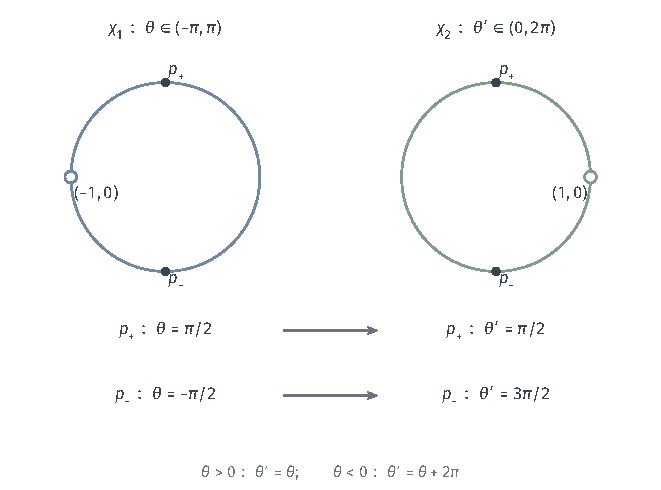
\includegraphics[width=112.0mm]{figures/01-mathematical-preliminaries-upper/02-linear-algebra-and-geometry/tikz/geometry-circle-chart-transition/figure.pdf}
  \caption{单位圆的两张坐标图。空心点分别是各图漏掉的$(-1,0)^\top$与$(1,0)^\top$，两图合起来覆盖完整圆。两图中的$p_+$相互对应，$p_-$也相互对应；每对标记记录同一个几何点。上半圆过渡保持角度，下半圆过渡加$2\pi$。图下方列出两个交叠分支的转换，不把坐标断点理解为圆被切断。}
  \label{fig:geometry-circle-chart-transition}
\end{figure}




同一个点在两张图中的坐标不同，过渡映射必须把旧记录送到新记录。
三张图共同覆盖时，$\chi_3\circ\chi_1^{-1}
=(\chi_3\circ\chi_2^{-1})\circ(\chi_2\circ\chi_1^{-1})$，
等式只在各步都有定义的重叠区域使用。与线性换基相同，中间记录消去；
不同之处在于过渡通常非线性且只在局部有效。

\section{关系与结构}
\label{sec:geometry-relations}

两条圆弧在小邻域中都可以用一个坐标记录，却可能属于不同的连通分支；
同一圆上的两点也有不同切线。局部坐标之外，还需建立邻域、切向与距离关系，
分别描述连续连接、可行速度与路线代价。若任务要忽略旋转或重编号，再以等价关系规定这种忽略。

\subsection{对象的邻域关系}
\label{sec:geometry-neighborhood-relations}
\label{sec:geometry-local-relations-topology}

\label{sec:geometry-neighborhood-topology}

在嵌入模型中，$\mathcal M\cap O$（$O$为环境开集）给出相对开集。
包含一个含有该点的相对开集的集合，称为该点的邻域。开集的任意并、有限交仍开，
它们决定连续映射、连通与局部记录所需的关系。
两条互不相交的开圆弧和一条完整圆，每个点附近都像一维开区间，
整体却分别有两个连通分支和一个不可在圆内缩到点的环。
\term{拓扑}（topology）在这里研究连续连接与孔洞等结构，
不要求保持长度和角度。把开点带连续拉直可以保留连接关系，
把两端粘合却改变了对象。局部自由度不能回答这种整体问题。

有限欧氏点集继承的拓扑是离散的；要从样本推测连续形状，必须额外选择哪些邻域算相连。
而一圈边是否被填满又不是成对连边能够决定的。为使$k+1$个顶点确实张成$k$维形状，
要求以一个顶点$\bm v_0$为基点时，差向量
$\bm v_1-\bm v_0,\ldots,\bm v_k-\bm v_0$线性无关；
这称为顶点的仿射独立（affine independence），三个顶点时就是不共线。
$k$维\term{单纯形}（simplex）在几何上是这些顶点的凸包，在组合表示中只记录顶点集合。
点、线段、填充三角形分别是零、一、二维单纯形。
仿射独立保证几何维数；组合形式则用于指定哪些高阶面存在。

\begin{definition}[抽象单纯复形]
\label{def:geometry-simplicial-complex}
有限顶点集上的\term{抽象单纯复形}（abstract simplicial complex）
$\mathcal K$是一族非空顶点子集，满足向下封闭：
\begin{equation}
 \sigma\in\mathcal K,\quad\varnothing\neq\tau\subseteq\sigma
 \quad\Longrightarrow\quad\tau\in\mathcal K.
 \label{eq:geometry-simplicial-complex-closure}
\end{equation}
含$k+1$个顶点的元素称为$k$维单纯形。
\end{definition}
加入三角面必须连同它的三条边和三个顶点一起加入，反之不成立。
这使复形能够区分“围出一圈”和“这一圈已由一个面填充”。


为计算未被填充的环，需要把端点抵消与高阶填充分别记录。
选定顶点次序后，以$[v_0,\ldots,v_k]$表示有向单纯形，交换两顶点使符号反转。
有向$k$维单纯形的实系数线性组合称为$k$维链，
组成向量空间$C_k(\mathcal K;\mathbb R)$。边界算子读取每个面的有向边缘：
\begin{equation}
 \partial_k[v_0,\ldots,v_k]
 =\sum_{i=0}^k(-1)^i[v_0,\ldots,\widehat{v_i},\ldots,v_k],
 \qquad k\geq1,
 \label{eq:geometry-simplicial-boundary}
\end{equation}
尖帽表示删去该顶点，算子线性延伸到全部链。
本章采用非约化同调，约定$C_{-1}=\{0\}$、$\partial_0=0$。
例如$\partial_1[1,2]=[2]-[1]$，端点的正负表示方向。

\begin{lemma}[边界的边界为零]
\label{lem:geometry-boundary-squared-zero}
上述算子满足
\begin{equation}
 \partial_{k-1}\partial_k=0,\qquad k\geq1.
 \label{eq:geometry-boundary-squared-zero}
\end{equation}
\end{lemma}
\begin{proof}
$k=1$时由$\partial_0=0$成立。对$k\geq2$，固定$i<j$，
两次删除$v_i,v_j$后得到相同的$(k-2)$维面。
先删$i$再删原来的$j$，系数为$(-1)^i(-1)^{j-1}$；
先删$j$再删$i$，系数为$(-1)^j(-1)^i$，两者相反。
所有项都按这样的顶点对成对抵消，因此结论对基单纯形成立；
由线性性，对全部链成立。
\end{proof}

边界必定闭合，但闭合的圈未必由复形中的某个面填充。
这正好可以用上一章的核、像与商空间表达。
\begin{definition}[闭链、边界与同调空间]
\label{def:geometry-homology-space}
满足$\partial_kc=0$的链称为\term{闭链}（cycle），
能写成$c=\partial_{k+1}b$的链称为\term{边界}（boundary）。
由$\partial_k\partial_{k+1}=0$，有
$\operatorname{im}\partial_{k+1}\subseteq\ker\partial_k$。
实系数\term{同调空间}（homology space）及其维数定义为
\[
 H_k(\mathcal K;\mathbb R)=\ker\partial_k/\operatorname{im}\partial_{k+1},
 \qquad \beta_k=\dim H_k(\mathcal K;\mathbb R).
\]
$\beta_k$称为第$k$个\term{Betti数}（Betti number）。
\end{definition}
商空间沿用定义~\ref{def:linear-algebra-quotient-space}：
两个闭链相差一个边界时被视为同类。因而$H_k$保留的不是全部闭链，
而是无法用已有高阶填充消去的部分；$\beta_0$计算连通分支，
$\beta_1$计算实系数意义下独立的一维环。

取
$\mathcal K_{\mathrm{loop}}
=\{\{1\},\{2\},\{3\},\{1,2\},\{2,3\},\{1,3\}\}$。
链$c=[1,2]+[2,3]-[1,3]$的端点逐一抵消，故$\partial_1c=0$。
$\partial_1$的秩为$2$，一维闭链空间维数为$3-2=1$，
而没有二维面，故$\beta_1=1$、$\beta_0=3-2=1$。
加入$[1,2,3]$后，$c=\partial_2[1,2,3]$成为边界，$\beta_1$降为$0$；
$\partial_1$不变，所以$\beta_0$仍为$1$。
图~\ref{fig:geometry-cycle-filled-simplex}只改变面集合，顶点与边保持相同。
\begin{figure}[htbp]
  \centering
  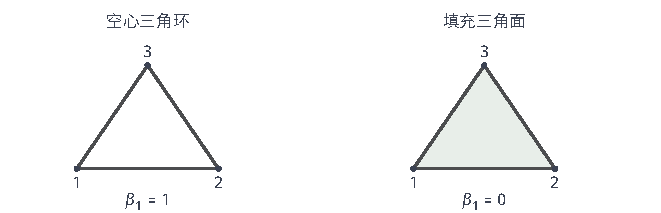
\includegraphics[width=112.0mm]{figures/01-mathematical-preliminaries-upper/02-linear-algebra-and-geometry/tikz/geometry-cycle-filled-simplex/figure.pdf}
  \caption{一圈边是否已填充，取决于高阶面而非边图。左侧闭链
 $c=[1,2]+[2,3]-[1,3]$不是边界；右侧加入$[1,2,3]$后有
 $c=\partial_2[1,2,3]$。两者$\beta_0=1$，$\beta_1$分别为$1$与$0$。
 图为组合教学示例，不代表某个观测点云的真实拓扑。}
 \label{fig:geometry-cycle-filled-simplex}
\end{figure}


若$N_k$是$k$维单纯形数，Euler示性数
$\chi=\sum_k(-1)^kN_k$是更粗的摘要：空心三角形为$3-3=0$，
填充三角形为$3-3+1=1$。由秩--零度关系
$N_k=\beta_k+\operatorname{rank}\partial_k+\operatorname{rank}\partial_{k+1}$，
交替求和后中间秩抵消，也得到$\chi=\sum_k(-1)^k\beta_k$。
不同Betti数组甚至不同拓扑都可能有同一个$\chi$，一个标量不足以代替分别分析。

\subsection{对象的位置与方向关系}
\label{sec:geometry-position-direction-relations}
\label{sec:geometry-manifold-local-linearization}
\label{sec:geometry-analytic-local-linearization}

从$\bm p=\varphi(\bm z)$出发，坐标变化$\bm v$经Jacobian
$\bm J_\varphi(\bm z)$映为环境空间中的瞬时速度。
\term{切空间}（tangent space）收集所有这样的可行速度；
它描述一阶方向，并不是可行集合本身的一小块。

\begin{definition}[嵌入流形的切空间]
\label{def:geometry-tangent-space}
设$\varphi:U\subseteq\mathbb R^d\to\mathcal M\subseteq\mathbb R^D$
是局部参数化，$\bm p=\varphi(\bm z)$。定义
\begin{equation}
 T_{\bm p}\mathcal M
 =\{\bm J_\varphi(\bm z)\bm v:\bm v\in\mathbb R^d\}.
 \label{eq:geometry-tangent-space-chart}
\end{equation}
\end{definition}
Jacobian列满秩保证这是$d$维向量空间，其原点是零速度。
画在$\bm p$旁边的仿射切平面则是$\bm p+T_{\bm p}\mathcal M$；
点的位置与速度向量的零点不能混为一谈。

\begin{lemma}[曲线速度与坐标刻画相容]
\label{lem:geometry-tangent-curves}
$T_{\bm p}\mathcal M$恰是全部光滑曲线
$\gamma:(-\epsilon,\epsilon)\to\mathcal M$、$\gamma(0)=\bm p$
的速度$\gamma'(0)$组成的集合，并且与局部坐标选择无关。
\end{lemma}
\begin{proof}
在足够小的参数区间内，曲线落入当前坐标图，写成
$\gamma(t)=\varphi(\bm z(t))$。链式法则给出
$\gamma'(0)=\bm J_\varphi(\bm z)\bm z'(0)$，故每个曲线速度都属于所定义的空间。
反过来，任意$\bm v\in\mathbb R^d$给出曲线
$t\mapsto\varphi(\bm z+t\bm v)$；因为$U$开，足够小的$t$仍在定义域内，
其初速度为$\bm J_\varphi(\bm z)\bm v$。

若另一参数化满足$\widetilde\varphi=\varphi\circ\psi$，
坐标过渡$\psi$的Jacobian可逆，且
$\bm J_{\widetilde\varphi}=\bm J_\varphi\bm J_\psi$。
右乘可逆矩阵不改变值域，两张图因而给出同一切空间。
\end{proof}

在点带中直接求导，可核对两个自由度：
\begin{align}
 \frac{\partial\Phi}{\partial s}
 &=\left(1+\frac uR\right)
   \begin{bmatrix}-\sin(s/R)\\\cos(s/R)\end{bmatrix},
 \label{eq:geometry-strip-s-tangent}\\
 \frac{\partial\Phi}{\partial u}
 &=\begin{bmatrix}\cos(s/R)\\\sin(s/R)\end{bmatrix}.
 \label{eq:geometry-strip-u-tangent}
\end{align}
因$|u|<w<R$，第一列不为零，两列正交且线性无关；
开带的切空间是整个$\mathbb R^2$。中心线则只允许$u=0$，
\[
 T_{\Phi(s,0)}\mathcal C
 =\operatorname{span}\{(-\sin(s/R),\cos(s/R))^\top\}.
\]
径向方向对开带可行，对中心线不可行。中心线的切线随位置转动，
没有一条固定线性子空间等于各处的切空间。

图~\ref{fig:geometry-strip-tangent-coordinates}上半部把切向速度画在点旁，
下半部比较同一坐标增量对应的实际弧长。方向数目决定局部维数，
坐标增量怎样换算为长度则留待度量处理。
\begin{figure}[htbp]
  \centering
  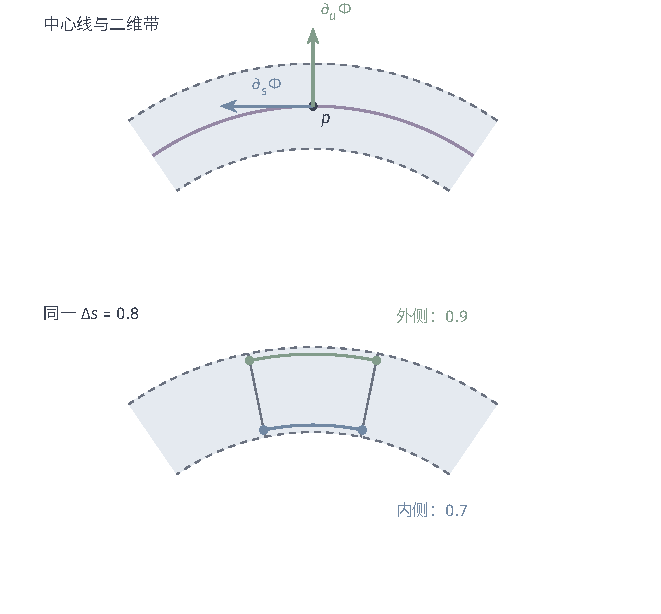
\includegraphics[width=112.0mm]{figures/01-mathematical-preliminaries-upper/02-linear-algebra-and-geometry/tikz/geometry-strip-tangent-coordinates/figure.pdf}
  \caption{开带与中心线的局部方向不同。取$R=2$、$w=0.3$。
 上图的两个参数方向属于二维开带，仅以中心线为对象时，径向方向不属于其切空间；
 箭头平移到$\bm p$只是画法。下图取$u=-0.25,0.25$，同一$\Delta s=0.8$
 对应圆弧长度$0.7,0.9$。灰虚线为不纳入开带的边界，两图等比例绘制，均为解析教学示例。}
 \label{fig:geometry-strip-tangent-coordinates}
\end{figure}


若流形由约束$F(\bm x)=\bm0$给出，其中
$F:\mathbb R^D\to\mathbb R^{D-d}$在$\bm p$附近光滑且
$\bm J_F(\bm p)$行满秩，就能选出$D-d$列组成可逆方阵。
重排坐标后，定理~\ref{thm:analysis-implicit-function}把这$D-d$个变量
解为其余$d$个变量的光滑函数，后者便给出局部参数化。
对约束内曲线求导得$\bm J_F(\bm p)\gamma'(0)=\bm0$；
所以切空间包含于该矩阵的核。参数化给出$d$维切空间，
秩--零度关系又说明核为$d$维，故$T_{\bm p}\mathcal M=\ker\bm J_F(\bm p)$。
满秩条件不能省略：$F(x,y)=x^2+y^2$在原点导数为零，
核是整个平面，但零水平集只有一个点，真实可行速度只有零向量。

\subsection{对象的距离关系}
\label{sec:geometry-metric-length-distance}
\label{sec:geometry-metric-path-geodesic}
\label{sec:geometry-same-point-metric}

\label{sec:geometry-riemannian-metric}
\label{sec:geometry-path-speed-length}
\label{sec:geometry-endpoint-distance}
\label{sec:geometry-continuous-geodesic-distance}

切空间说明方向可不可行，却没有规定一单位坐标变化有多长。
点带外侧与内侧相同的$\mathrm ds$对应不同弧长，因而内积必须按位置指定。
\term{Riemann度量}（Riemannian metric）为每个切空间提供这种长度与夹角规则。

在局部参数化$\varphi$中，把坐标记为$(z^1,\ldots,z^d)$；
上标在这里是坐标编号。相应坐标切基为
$\partial_i=\partial\varphi/\partial z^i$。

\begin{definition}[Riemann度量]
\label{def:geometry-riemannian-metric}
光滑流形$\mathcal M$上的Riemann度量$g$为每个$\bm p$指定内积
$g_{\bm p}:T_{\bm p}\mathcal M\times T_{\bm p}\mathcal M\to\mathbb R$，
且在任一光滑坐标切基$\partial_i$中，矩阵
$\bm G(\bm z)=[g_{i,j}(\bm z)]$、$g_{i,j}=g(\partial_i,\partial_j)$
的条目光滑。每个$\bm G$都对称正定。
\end{definition}
对同点切向量$\bm v,\bm w$，长度为
$\lVert\bm v\rVert_g=\sqrt{g_{\bm p}(\bm v,\bm v)}$；
非零时夹角满足
$\cos\vartheta=g_{\bm p}(\bm v,\bm w)/
(\lVert\bm v\rVert_g\lVert\bm w\rVert_g)$。
若它们的坐标分量为$\bm a,\bm b$，内积是$\bm a^\top\bm G\bm b$。
$\bm G$既不是样本协方差，也不必是全空间共享的常矩阵。

嵌入流形可以限制环境欧氏内积，得到诱导度量：
\begin{equation}
 \bm G(\bm z)=\bm J_\varphi(\bm z)^\top\bm J_\varphi(\bm z).
 \label{eq:geometry-induced-metric}
\end{equation}
对非零$\bm a$，满列秩保证
$\bm a^\top\bm G\bm a=\lVert\bm J_\varphi\bm a\rVert_2^2>0$。
若Jacobian退化，只会得到半正定形式；这不符合当前坐标中的Riemann度量条件。
也可以另选光滑正定内积，但这样会改变几何，而不只是改写坐标。

若旧坐标$\bm z=\psi(\bm v)$，记可逆Jacobian为$\bm A=\bm J_\psi$，
同一几何向量的旧分量等于$\bm A$乘新分量，所以
\begin{equation}
 \widetilde{\bm G}(\bm v)=
 \bm A^\top\bm G(\psi(\bm v))\bm A.
 \label{eq:geometry-metric-coordinate-transform}
\end{equation}
因此$\bm a^\top\widetilde{\bm G}\bm b
=(\bm A\bm a)^\top\bm G(\bm A\bm b)$。
改变分量而不改变度量会改变所计算的长度；按此式一起变换则仍描述同一内积。

点带的两个参数方向已在式~\eqref{eq:geometry-strip-s-tangent}与
\eqref{eq:geometry-strip-u-tangent}中求出，故
\begin{equation}
 \bm G(s,u)=
 \begin{bmatrix}(1+u/R)^2&0\\0&1\end{bmatrix}.
 \label{eq:geometry-strip-metric}
\end{equation}
横向速度$\dot u$的长度系数为$1$，纵向速度$\dot s$的系数为$1+u/R$。
在$R=2$、$u=\pm0.25$时，同一$\Delta s=0.8$沿固定$u$的圆弧
分别产生$0.9$与$0.7$的长度，与图~\ref{fig:geometry-strip-tangent-coordinates}一致。
内积权重来自坐标尺度，并不由该位置采到了多少点决定。


设分段光滑路径$\gamma:[a,b]\to\mathcal M$在一张图中写成
$\gamma(t)=\varphi(\bm z(t))$。链式法则保证
$\dot\gamma(t)\in T_{\gamma(t)}\mathcal M$，度量读出的平方速度为
\begin{equation}
 \lVert\dot\gamma(t)\rVert_g^2
 =\dot{\bm z}(t)^\top\bm G(\bm z(t))\dot{\bm z}(t).
 \label{eq:geometry-riemannian-speed}
\end{equation}
将标量速度按时间累计，定义路径长度
\begin{equation}
 L_g(\gamma)=\int_a^b
 \sqrt{\dot{\bm z}(t)^\top\bm G(\bm z(t))\dot{\bm z}(t)}\,\mathrm dt.
 \label{eq:geometry-riemannian-curve-length}
\end{equation}
整条路径不在同一张图时，将紧区间$[a,b]$分成有限段，使每段落入一张图，
再求长度之和。紧致的路径像和坐标开覆盖保证能作这种有限分段。

这种计算不依赖坐标。在$\bm z=\psi(\bm v)$下，
$\dot{\bm z}=\bm A\dot{\bm v}$，
式~\eqref{eq:geometry-metric-coordinate-transform}给出
$\dot{\bm v}^\top\widetilde{\bm G}\dot{\bm v}
=\dot{\bm z}^\top\bm G\dot{\bm z}$。
每段被积的标量相同，所以重叠区域选哪张图、怎样进一步细分都不改变长度。

长度也不依赖沿同一路线前进的快慢。对保持方向的光滑重参数化$t=\tau(r)$，
新速度为$\dot\gamma(\tau(r))\tau'(r)$，
其长度因子为$|\tau'(r)|$；当$\tau'>0$时，
积分换元$\mathrm dt=\tau'(r)\mathrm dr$给出相同总长。
反向的光滑单调参数化配合积分端点互换也不改变长度。
允许停顿的分段正则重参数化可分段处理；来回多走则改变路线的经过次数，
不属于仅仅换速度。

瞬时切向可行不等于环境直线可行。单位圆上
$\bm p=(1,0)^\top$、$\bm v=(0,1)^\top\in T_{\bm p}\mathbb S^1$，
但$\lVert\bm p+t\bm v\rVert_2=\sqrt{1+t^2}>1$对$t\neq0$成立。
速度只描述路径的一阶变化，保持有限步可行仍需在曲面上构造完整路径或更新映射。


路径长度评价一条给定路线；端点间的距离则比较所有连接它们的允许路线。

\begin{definition}[测地距离]
\label{def:geometry-geodesic-distance}
在Riemann流形$(\mathcal M,g)$的同一路径连通分支内，定义
\term{测地距离}（geodesic distance）为连接两点的全部分段光滑路径长度的下确界：
\begin{equation}
 d_g(\bm p,\bm q)=
 \inf_{\substack{\gamma(a)=\bm p\\\gamma(b)=\bm q}}L_g(\gamma).
 \label{eq:geometry-geodesic-distance}
\end{equation}
若无连接路径，约定值为$+\infty$；在可能不连通的整个空间上，它是扩展距离。
\end{definition}
这里的定义尚不要求存在最短路径，更不依赖测地线方程。
反向路径给出对称性，拼接两条近似最短路径给出三角不等式。
对不同点$\bm p,\bm q$，取以$\bm p$为中心、闭包仍在坐标图内且不含
$\bm q$的小坐标球。度量在这个闭球内有正的下界；任何连接两点的路径都必须
先到达球的边界，因而已经付出一个正的长度。不同点的距离为正，
所以每个连通分支中确实得到度量。

对于欧氏诱导度量，由
$\bm q-\bm p=\int_a^b\dot\gamma(t)\,\mathrm dt$与三角不等式，
每条连接路径均满足$\lVert\bm q-\bm p\rVert_2\leq L_g(\gamma)$，
所以
\[
 \lVert\bm q-\bm p\rVert_2\leq d_g(\bm p,\bm q).
\]
若连接线段完全可行，就取等。反过来，只有下确界被允许路径达到时，
取等才迫使该最短路径沿线段行进，至多改变速度；
距离相等本身不保证线段可行。若换成任意非诱导度量，上述环境距离比较也不能照搬。

回到开中心线的两点$\bm p=\Phi(s,0)$、$\bm q=\Phi(t,0)$。
环境空间的弦长是
\begin{equation}
 \lVert\Phi(s,0)-\Phi(t,0)\rVert_2
 =2R\left|\sin\frac{s-t}{2R}\right|.
 \label{eq:geometry-strip-chord-distance}
\end{equation}
中心线以$s$为弧长参数，允许路径必须留在开弧内，因此
$d_{\mathcal C}(\bm p,\bm q)=|s-t|$。
二维带允许路径向内侧绕行，中心线弧只是候选，故
\[
 \lVert\bm p-\bm q\rVert_2
 \leq d_{\mathcal M_{\mathrm{strip}}}(\bm p,\bm q)
 \leq d_{\mathcal C}(\bm p,\bm q)=|s-t|.
\]
带宽、端点位置和允许域决定第二个不等式是否严格；
不能把这两种距离都称为不加区分的“沿带距离”。

另取完整单位圆作为独立例子。夹角$0\leq\theta\leq\pi$时，
允许选择短弧，内在距离为$\theta$，弦长为$2\sin(\theta/2)$。
在$\theta=\pi/2$时两者为$\pi/2$与$\sqrt2$；
小角度展开$2\sin(\theta/2)=\theta-\theta^3/24+O(\theta^5)$说明局部接近，
全局却不同。图~\ref{fig:geometry-circle-distances}在相同尺度上比较这两种量。
\begin{figure*}[htbp]
  \centering
  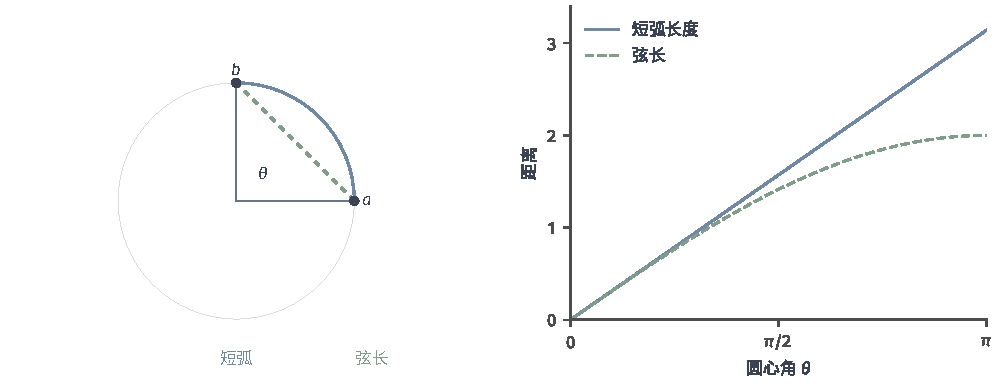
\includegraphics[width=169.0mm]{figures/01-mathematical-preliminaries-upper/02-linear-algebra-and-geometry/matplotlib/geometry-circle-distances/figure.pdf}
  \caption{完整单位圆的测地距离与环境弦长。左图夹角为$\pi/2$，
 蓝线为圆上的允许短弧，绿虚线为穿过圆内的环境线段；
 右图比较$\theta\in[0,\pi]$时的两种长度。完整圆允许选择两段弧中的较短者，
 不能与开中心线或二维开带的允许路径混用。图为解析教学示例。}
 \label{fig:geometry-circle-distances}
\end{figure*}

定义使用下确界是有意保留存在性问题。在穿孔平面
$\mathbb R^2\setminus\{\bm0\}$中，$(-1,0)^\top$与$(1,0)^\top$
之间可绕过任意小的圆孔，路径长度趋于$2$，却没有长度恰为$2$的允许路径。
哪些全局条件保证达到下确界，将在固定端点的最短路径问题中讨论。

\subsection{对象的等价关系}
\label{sec:geometry-equivalence-relations}
\label{sec:geometry-symmetry-group-actions}

坐标可改变，不意味着任务输出必须不变。整体旋转点带时，长度不变，
表示朝向的向量却应同步旋转；重排点记录的行，则只改变编号而不移动空间中的点。
要准确规定这些要求，先明确允许哪些变换、如何复合，再指定它们作用于什么对象。

\begin{definition}[群]
\label{def:geometry-group}
\term{群}（group）$G$是带有二元运算的集合。运算封闭且满足结合律，
存在恒等元$e$，每个$g\in G$都存在逆元$g^{-1}$。
\end{definition}
群描述可以接连施加、也可以撤销的变换规则。集合中若只有若干增强操作，
复合后不再属于该集合，或者裁剪已丢失信息而不可逆，就还不能直接称其为群。
群的抽象乘法与对象上的实际操作，通过群作用联系。

\begin{definition}[群作用]
\label{def:geometry-group-action}
\term{群作用}（group action）是映射$G\times\mathcal X\to\mathcal X$，
记$(g,x)\mapsto g\cdot x$，满足
\begin{equation}
 e\cdot x=x,\qquad (g_1g_2)\cdot x=g_1\cdot(g_2\cdot x)
 \label{eq:geometry-group-action}
\end{equation}
对所有$x\in\mathcal X$和$g_1,g_2\in G$成立。
\end{definition}
第二条把群乘法解释为先做$g_2$、再做$g_1$。
同一个群可以作用在不同空间上，具体作用必须给出；讨论光滑流形上的作用时，
还要另行要求相应映射光滑。


如果任务确实要忽略某类变换，就应把该变换关联的输入视为等价。
\term{轨道}（orbit）$G\cdot x=\{g\cdot x:g\in G\}$收集从$x$出发能够得到的
所有输入。定义$x\sim y$当且仅当存在$g\in G$使$y=g\cdot x$，这是等价关系：
恒等元保证反身，逆元保证对称，复合保证传递。轨道的集合称为轨道商$\mathcal X/G$。
这时才有明确依据说两个不同记录代表同一个等价输入。


轨道商在这里只是等价类集合。即使原空间光滑，也不能直接宣布商仍是同维或更低维
的光滑流形。例如平面上全部旋转组成的群$\mathrm{SO}(2)$作用于$\mathbb R^2$，
轨道按半径标记，
商可识别为$[0,\infty)$：原点的轨道只有一个点，其余轨道是圆。
商的端点不满足无边界一维流形的局部开区间条件。若讨论一般商的光滑结构，
需要补充作用的正则性条件，不能仅凭“去掉一个旋转自由度”作维数相减。

\section{运算与映射}
\label{sec:geometry-operations}

位置映射将一个点送到另一个点或一组特征，映射的叠加与复合组织多步作用。
点一旦变化，还需说明速度怎样传递、旧方向怎样搬到新位置，以及怎样从切向步产生可行的新点。
最后再从度量计算区域体积，为下一章的函数积分提供几何权重。

\subsection{空间之间的映射}
\label{sec:geometry-point-maps}

圆上位置可以映到横坐标，也可以映到另一个曲面上的位置。
要判断这样的映射是否光滑，先把两端位置都转成局部欧氏坐标。
设$F:\mathcal M\to\mathcal N$，用输入参数化$\varphi$与输出参数化$\psi$
记录后，$\psi^{-1}\circ F\circ\varphi$是欧氏开集之间的映射。
若所有适用图中的表达都光滑，就称$F$光滑；光滑过渡和链式法则保证换图不改变这个判断。
输出也可以是$\mathbb R^r$中的特征，而不一定是另一个弯曲空间中的位置。
例如单位圆上的$(x,y)\mapsto x$读取环境横坐标，仍是合法的光滑映射。

\subsection{映射的叠加}
\label{sec:geometry-map-addition}

映射叠加要求各分支具有共同定义域，输出落在同一个可加的线性空间。
若$F_j:\mathcal M\to V$、$a_j$固定，则
$F(p)=\sum_j a_jF_j(p)$定义新的映射；各分支光滑时，坐标表达逐项相加仍光滑。
这里不要求$\mathcal M=V$。若输出是球面位置，直接相加通常不再可行；
若另作归一化，还须排除和为零，并把归一化看作新的复合步骤。

点云分支可以各自接收整幅点云，再把同形特征相加；共享逐点分支也可以先产生
各点特征，再求和汇聚。两者的输入对象不同，不能仅凭代码中都有求和就视为同一个作用。

\subsection{映射的复合}
\label{sec:geometry-map-composition}
\label{sec:geometry-group-invariance-equivariance}


当$F:\mathcal M\to\mathcal N$、$H:\mathcal N\to\mathcal P$的中间对象匹配时，
$(H\circ F)(p)=H(F(p))$。下面用复合表达变换后的响应：
保持数值是不变性，按指定方式改变输出是等变性。
当对象是向量且作用保持线性组合时，可以直接用线性代数描述响应。
\begin{definition}[线性表示]
\label{def:geometry-linear-representation}
\term{线性表示}（linear representation）是映射
$\rho:G\to\operatorname{GL}(V)$，满足
\begin{equation}
 \rho(e)=\bm I,\qquad \rho(g_1g_2)=\rho(g_1)\rho(g_2),
 \label{eq:geometry-linear-representation}
\end{equation}
其中$\operatorname{GL}(V)$是向量空间$V$上全部可逆线性算子组成的群。
\end{definition}
它用线性算子实现群的复合规则。输入与输出可以取不同表示：
输入平面坐标按旋转矩阵变换，标量输出可以取$\rho(g)=1$，
方向向量输出则可取同一旋转矩阵。

平面旋转群$\mathrm{SO}(2)$由行列式为$1$的二维正交矩阵组成。
角度$\theta$对应
\begin{equation}
 \bm R(\theta)=
 \begin{bmatrix}\cos\theta&-\sin\theta\\\sin\theta&\cos\theta\end{bmatrix},
 \qquad
 \bm R(\theta_1)\bm R(\theta_2)=\bm R(\theta_1+\theta_2).
 \label{eq:geometry-planar-rotation-group}
\end{equation}
同一旋转可作用于一个点、整组点，或通过改变自变量作用于图像函数。
这些输入空间不同。对点带整体旋转时，坐标写成$\bm R(\theta)\Phi(s,u)$，
局部参数$(s,u)$可以不变；这是环境表示改变，并非必须重新定义内部位置。

有限集合$\{1,\ldots,n\}$的全部置换组成对称群$S_n$。
约定置换矩阵满足$(\bm P_\pi\bm X)_{i,:}=\bm X_{\pi^{-1}(i),:}$，
则$\bm P_{\pi_1\pi_2}=\bm P_{\pi_1}\bm P_{\pi_2}$。
对点云$\bm X\in\mathbb R^{n\times D}$，行置换改变记录顺序，
而$D$维旋转矩阵$\bm R$作用在坐标列上，写为$\bm X\bm R^\top$。矩阵乘法的外形相似，
实际被改变的对象和索引却不同。


\begin{definition}[不变映射]
\label{def:geometry-invariant-map}
群$G$作用于$\mathcal X$。映射$f:\mathcal X\to\mathcal Y$若满足
\begin{equation}
 f(g\cdot x)=f(x)\qquad(g\in G,\ x\in\mathcal X),
 \label{eq:geometry-invariant-map}
\end{equation}
称为对该作用\term{不变}（invariant）。
\end{definition}
不变映射在同一轨道上取相同值，因此可写成
$f=\widetilde f\circ\pi$，其中$\pi(x)=G\cdot x$是商映射。
令$\widetilde f(G\cdot x)=f(x)$之所以不依赖代表元，正是由不变性保证。
但$f$也可能把不同轨道映到同一输出；不变不等于保留了区分轨道的全部信息。


当输出必须保留位置或朝向时，合理要求是让它按约定同步变化。
\begin{definition}[等变映射]
\label{def:geometry-equivariant-map}
若$G$还作用于$\mathcal Y$，把输出作用记为$\rho(g)$，映射
$F:\mathcal X\to\mathcal Y$满足
\begin{equation}
 F(g\cdot x)=\rho(g)F(x)\qquad(g\in G,\ x\in\mathcal X),
 \label{eq:geometry-equivariant-map}
\end{equation}
则称为\term{等变}（equivariant）。输出作用不必线性；当$\mathcal Y$是向量空间
且$\rho$为线性表示时，右端才是相应线性算子的作用。
\end{definition}
例如预测点带朝向时，输入旋转后，输出向量也应旋转。
标量类别、位置坐标和分割掩码所需的响应不同，不变性不是比等变性更好的统一目标。
等变映射之后接不变汇总可得到不变输出；反过来，已丢弃朝向的信息通常不能恢复。

在点云上，对每行使用同一个映射$\phi$，令
$F(\bm X)_{i,:}=\phi(\bm X_{i,:})$，则第$i$行直接给出
\[
 F(\bm P_\pi\bm X)_{i,:}
 =\phi(\bm X_{\pi^{-1}(i),:})
 =(\bm P_\pi F(\bm X))_{i,:}.
\]
所以逐点共享映射对行置换等变。再对行求和，
$f(\bm X)=\sum_i\phi(\bm X_{i,:})$，重编号只改变求和次序，因而不变。
这证明了响应关系，尚未证明求和表示能够区分任务需要的全部点集。

平移作用的例子需要同时规定定义域。对全空间上的可积函数
$k,f\in L^1(\mathbb R^d)$，这里$L^1$表示绝对值积分有限的函数。
令$(T_{\bm a}f)(\bm x)=f(\bm x-\bm a)$，
卷积是将一个函数平移后与另一个相乘并积分：
\begin{align}
 (k*(T_{\bm a}f))(\bm x)
 &=\int_{\mathbb R^d}k(\bm x-\bm y)f(\bm y-\bm a)\,\mathrm d\bm y\\
 &=\int_{\mathbb R^d}k(\bm x-\bm a-\bm z)f(\bm z)\,\mathrm d\bm z
   =(T_{\bm a}(k*f))(\bm x).
 \label{eq:geometry-translation-convolution-equivariance}
\end{align}
变量替换$\bm z=\bm y-\bm a$说明卷积与平移可交换。
$L^1$条件使等式几乎处处成立，即除去一个Lebesgue零测集后成立。
若积分处处绝对收敛，例如一个函数连续有界、
另一个可积，就可以逐点理解。有限图像的零填充、裁剪和下采样可能破坏所声称的
平移等变性；循环平移配周期边界和只比较有效区域又是另外的作用，须逐项核对。

\begin{table*}[htbp]
 \centering\small
 \begin{tabularx}{\linewidth}{@{}lXX@{}}
 \toprule
 输入作用 & 不变输出 & 等变输出及其作用\\
 \midrule
 平面旋转$\bm x\mapsto\bm R\bm x$
 & $\lVert\bm x\rVert_2$ & $F(\bm x)=\bm x$，输出也乘$\bm R$\\
 点记录行置换$\bm X\mapsto\bm P\bm X$
 & 逐行映射后求和 & 逐行共享映射，输出行也乘$\bm P$\\
 全空间信号平移
 & 可积函数的全空间积分 & 与固定可积核卷积，输出信号同样平移\\
 \bottomrule
 \end{tabularx}
 \caption{先指定输入与输出作用，才能判断不变或等变。全空间信号的恒等式不自动适用于
 有裁剪、边界填充或下采样的有限窗口；结构响应也不保证表示保留了任务所需的全部信息。}
 \label{tab:geometry-invariance-equivariance}
\end{table*}
表~\ref{tab:geometry-invariance-equivariance}把同一个输入作用的两种输出要求并列，
区别在于输出应该忽略变换，还是记录变换后的对象。


群复合还可以构造相对位置表示。对实数位置$t$和频率$\omega$，
令$\bm R_\omega(t)=\bm R(\omega t)$。同时平移位置$s,t$不改变$t-s$，而旋转复合给出
\begin{equation}
 \bm R_\omega(s)^\top\bm R_\omega(t)=\bm R_\omega(t-s).
 \label{eq:geometry-rotary-relative-position}
\end{equation}
所以对固定二维向量$\bm q,\bm k$，
\begin{equation}
 (\bm R_\omega(s)\bm q)^\top(\bm R_\omega(t)\bm k)
 =\bm q^\top\bm R_\omega(t-s)\bm k.
 \label{eq:geometry-rotary-dot-product}
\end{equation}
多个频率块并置仍保留这一恒等式，位置引入的旋转因子只通过相对位移出现。
这不意味着整个注意力网络只依赖相对位置：$\bm q,\bm k$的生成、其他位置特征、
偏置、窗口与边界仍可能含绝对位置信息。单个非零频率块的周期为$2\pi/|\omega|$，
多频率组合的可区分范围需连同频率、数值精度和序列长度分析，不能据此承诺无限长度
无碰撞。这里比较的是指定代数变换；后文沿曲面搬运方向还要给出路径和联络，
不能把两种操作都简化为一次任意旋转。


若要进一步组织可复合的局部表示，可以简要使用\term{范畴}（category）：
它包含对象、对象之间的箭头及各对象的恒等箭头，
仅在端点匹配时复合箭头，复合满足结合律与恒等律。
函子（functor）把对象和箭头映到另一范畴，同时保持恒等与复合。
例如坐标区域间可复合的过渡可按这种方式记录。
这只是组合表示的延伸语言，本章的距离与同调推导均不依赖它，
也不因引入这些名称获得额外的恢复保证。

\subsection{切向量的映射}
\label{sec:geometry-tangent-maps}

例如圆上的点在移动时，其横坐标也随之变化；给定点的瞬时速度，就应能计算读数的瞬时变化。
因此，除了点映射本身，还要建立它对切向速度的作用。
对第\ref{sec:geometry-point-maps}节定义的光滑映射$F:\mathcal M\to\mathcal N$，
取输入、输出两端的局部参数化$\varphi,\psi$。
它在$\bm p$处的微分（differential）把输入速度转成输出速度：
\[
 \mathrm dF_{\bm p}(\bm v)
 =\left.\frac{\mathrm d}{\mathrm dt}F(\gamma(t))\right|_{t=0},
 \qquad\gamma(0)=\bm p,\quad\gamma'(0)=\bm v.
\]
若$\bm v=\bm J_\varphi(\bm z)\bm a$，令
$\bm w=\psi^{-1}(F(\bm p))$，则
\begin{equation}
 \mathrm dF_{\bm p}(\bm v)
 =\bm J_\psi(\bm w)
   \bm J_{\psi^{-1}\circ F\circ\varphi}(\bm z)\bm a.
 \label{eq:geometry-map-differential}
\end{equation}
右端只依赖初速度，不依赖实现速度的曲线，因此定义良好且线性。
坐标变换时两侧的Jacobian因链式法则相互抵消；
$\mathrm dF_{\bm p}:T_{\bm p}\mathcal M\to T_{F(\bm p)}\mathcal N$
是几何映射，矩阵只是其坐标记录。复合还满足
$\mathrm d(H\circ F)_{\bm p}=\mathrm dH_{F(\bm p)}\circ\mathrm dF_{\bm p}$。

对标量函数$f:\mathcal M\to\mathbb R$，微分读取速度引起的一阶数值变化。
\term{余切空间}（cotangent space）$T_{\bm p}^*\mathcal M$就是
$T_{\bm p}\mathcal M$的线性泛函空间，泛函的含义沿用
第\ref{sec:linear-algebra-scalar-readouts}节的有限维标量读取。
有限维向量空间上的全部线性读取组成其对偶空间（dual space）；
所以$\mathrm df_{\bm p}\in T_{\bm p}^*\mathcal M$，不是一个切向量。
沿用前面的局部坐标$(z^1,\ldots,z^d)$与坐标切基$\partial_i$，
其对偶基$\mathrm dz^i$满足$\mathrm dz^i(\partial_j)=\delta_{i,j}$，
也就是$\mathrm dz^i(\sum_j a^j\partial_j)=a^i$：它读出速度的第$i$个坐标系数。于是
\[
 \mathrm df=\sum_i\partial_i(f\circ\varphi)\,\mathrm dz^i,\qquad
 \mathrm df\!\left(\sum_i a^i\partial_i\right)
 =\sum_i\partial_i(f\circ\varphi)a^i.
\]
例如圆上$f(\cos\theta,\sin\theta)=\cos\theta$，
角速度$a$对应的数值变化为$-a\sin\theta$。
要把这个线性读取规则表示成“最陡方向”，还须指定方向长度，
第\ref{sec:geometry-point-optimization}节将用已经建立的度量，把这个读取规则表示为梯度。

\subsection{切向量的搬运}
\label{sec:geometry-tangent-transport}
\label{sec:geometry-connection-comparison}
\label{sec:geometry-riemannian-curvature}

\label{sec:geometry-cross-point-comparison-curvature}
\label{sec:geometry-parallel-transport}

沿路径计算长度时，每个位置只输出一个标量。若要问速度有没有转弯，
或相邻两点的方向是否一致，就必须比较不同切空间中的向量。
即使流形嵌在同一个欧氏空间内，直接相减也可能产生法向分量：
圆上恒速运动的速度导数指向圆心，却没有沿圆加速。
需要把环境变化与流形内的方向变化分开。下面建立联络、平行移动和曲率，
所用的Riemann几何基础可参见Lee的教材\scite{math-lee2018riemannian}。


把圆周上的单位切向速度画在每个位置，得到一个向量场。
沿圆周求它的环境导数会出现法向分量，但流形内的方向变化应仍是切向的。
下面用联络规定这种微分：它保持切向性，也保留求导对加法与函数乘积的规则。
联络据此比较邻近位置的方向，无须把所有切空间认作同一个固定子空间。

\begin{definition}[向量场与联络]
\label{def:geometry-connection}
光滑\term{向量场}（vector field）$\bm V$在每个$\bm p\in\mathcal M$选取
$\bm V(\bm p)\in T_{\bm p}\mathcal M$，其坐标分量光滑。
\term{联络}（connection）为两个光滑向量场$\bm U,\bm V$指定向量场
$\nabla_{\bm U}\bm V$，称为$\bm V$沿$\bm U$的
\term{协变导数}（covariant derivative），并满足
\[
 \begin{aligned}
 \nabla_{f\bm U+h\bm W}\bm V
   &=f\nabla_{\bm U}\bm V+h\nabla_{\bm W}\bm V,\\
 \nabla_{\bm U}(a\bm V+b\bm W)
   &=a\nabla_{\bm U}\bm V+b\nabla_{\bm U}\bm W,\\
 \nabla_{\bm U}(f\bm V)
   &=\bm U(f)\bm V+f\nabla_{\bm U}\bm V.
 \end{aligned}
\]
其中$f,h$为光滑函数，$a,b\in\mathbb R$，
$\bm U(f)=\mathrm df(\bm U)$为方向导数。
\end{definition}
第一项对求导方向按光滑函数线性，第二项对被求导对象按常数线性，
第三项则说明不能把第二项也加强为按光滑函数线性：
系数本身的变化必须保留。欧氏空间的普通方向导数满足这三项规则；
一般流形上，单独求坐标分量的导数不够，因为坐标切基本身也在变。

度量已经规定长度，新的导数应当与这一判断相容。
此外，非坐标方向场先后作用的顺序本来就可能不同，不能把这种差异误认为额外的几何扭转。
定义交换子$[\bm U,\bm V]$为对任意光滑$f$满足
\[
 [\bm U,\bm V](f)=\bm U(\bm V(f))-\bm V(\bm U(f))
\]
的向量场；在坐标基下，其第$k$个分量为
$\sum_i(U^i\partial_iV^k-V^i\partial_iU^k)$。
坐标方向$\partial_i,\partial_j$的交换子为零，一般方向场则未必。

\begin{example}[平面上不可交换的方向场]
\label{ex:geometry-plane-field-commutator}
在欧氏平面取$\bm U=\partial_x$、$\bm V=x\partial_y$。
$\bm U$始终沿$x$轴，$\bm V$沿$y$轴但其大小随$x$改变。
对任意光滑函数$f$，
\[
 \bm U(\bm V(f))=\partial_yf+x\partial_x\partial_yf,\qquad
 \bm V(\bm U(f))=x\partial_y\partial_xf,
\]
故$[\bm U,\bm V]=\partial_y$。先沿$x$方向移动，会改变随后沿$\bm V$移动的速度；
两个方向场的顺序差异在平面上就会出现。
欧氏空间的普通方向导数还给出
\[
 \nabla_{\bm U}\bm V=\partial_y,\qquad
 \nabla_{\bm V}\bm U=\bm0.
\]
二者之差恰是交换子。这个平坦例子说明，方向场本身随位置变化所产生的差异，
需要与几何结构额外产生的差异分开。
\end{example}

\begin{definition}[Levi--Civita联络]
\label{def:geometry-levi-civita-connection}
给定Riemann度量$g$，同时满足下列度量相容与无挠条件的联络，
称为它的\term{Levi--Civita联络}（Levi--Civita connection）：
\begin{align*}
 \bm U\bigl(g(\bm V,\bm W)\bigr)
 &=g(\nabla_{\bm U}\bm V,\bm W)+g(\bm V,\nabla_{\bm U}\bm W),\\
 \nabla_{\bm U}\bm V-\nabla_{\bm V}\bm U&=[\bm U,\bm V].
\end{align*}
\end{definition}
度量相容使内积的求导仍满足乘积法则；无挠规定联络在交换两个方向场时，
不产生交换子之外的差异。无挠\emph{不}声称
$\nabla_{\bm U}\nabla_{\bm V}\bm W
=\nabla_{\bm V}\nabla_{\bm U}\bm W$，后者涉及本节末尾的曲率。

每个光滑Riemann度量唯一确定这样的联络。其唯一性可以从两项条件直接看出：
轮换$\bm U,\bm V,\bm W$的度量相容等式，并用无挠条件消去交换项，得到
\begin{align}
 2g(\nabla_{\bm U}\bm V,\bm W)
 &=\bm U g(\bm V,\bm W)+\bm V g(\bm W,\bm U)
   -\bm W g(\bm U,\bm V)\notag\\
 &\quad+g([\bm U,\bm V],\bm W)-g([\bm V,\bm W],\bm U)
   +g([\bm W,\bm U],\bm V).
 \label{eq:geometry-koszul-formula}
\end{align}
右端只含已知度量、向量场和普通方向导数；正定性使其唯一确定
$\nabla_{\bm U}\bm V$。反过来，用此式定义该向量场，代入可检查联络的三条规则、
度量相容和无挠条件，因而也给出存在性。这个公式的用途是确定比较规则，
实际计算通常使用坐标系数或环境投影。

对继承欧氏度量的嵌入流形，设$\bm P_{\bm p}$为环境空间到
$T_{\bm p}\mathcal M$的正交投影，则
\begin{equation}
 \nabla_{\bm U}\bm V(\bm p)
 =\bm P_{\bm p}\,\mathrm d\bm V_{\bm p}(\bm U(\bm p)).
 \label{eq:geometry-projected-connection}
\end{equation}
这里把$\bm V$视为取值于环境$\mathbb R^D$的映射，先求环境导数再投影。
投影保持对切向量的内积，所以欧氏内积的乘积法则给出度量相容；
环境方向导数之差是已经切向的交换子，投影后仍不变，故也无挠。
由唯一性，这正是诱导度量的Levi--Civita联络。
若度量不是环境诱导度量，不能继续沿用这个欧氏正交投影公式。


现在固定路径$\gamma(t)$和起点切向量，希望沿路保持方向。
“保持”不是要求环境坐标分量不变，而是要求联络测得的变化为零。
在坐标基中写
$\nabla_{\partial_i}\partial_j=\sum_k\Gamma^k_{i,j}\partial_k$。
这些系数称为Christoffel符号，记录坐标切基随位置的变化；第\ref{sec:geometry-position-updates}节将从度量求出其表达式。
沿$\gamma(t)=\varphi(\bm z(t))$的向量
$\bm V(t)=\sum_jV^j(t)\partial_j$满足
\begin{equation}
 \frac{D\bm V}{\mathrm dt}
 =\sum_k\left(\dot V^k+
     \sum_{i,j}\Gamma^k_{i,j}(\bm z(t))\dot z^iV^j\right)\partial_k.
 \label{eq:geometry-covariant-derivative-along-path}
\end{equation}
第一项是分量变化，第二项修正坐标切基的变化；合起来才是坐标无关的协变导数。
对于欧氏诱导度量，式~\eqref{eq:geometry-projected-connection}沿路径写成
\[
 \frac{D\bm V}{\mathrm dt}
 =\bm P_{\gamma(t)}\frac{\mathrm d\bm V}{\mathrm dt},
\]
保留环境导数的切向部分。

\begin{definition}[平行移动]
\label{def:geometry-parallel-transport}
给定分段光滑路径$\gamma:[a,b]\to\mathcal M$和
$\bm v\in T_{\gamma(a)}\mathcal M$，沿路解
\[
 \frac{D\bm V}{\mathrm dt}=\bm0,\qquad \bm V(a)=\bm v.
\]
终值定义线性映射
$P_\gamma:T_{\gamma(a)}\mathcal M\to T_{\gamma(b)}\mathcal M$，
称为沿$\gamma$的\term{平行移动}（parallel transport）。
\end{definition}
坐标式是具有连续系数的线性常微分方程，初值唯一决定解；
沿有限段路径逐图求解并拼接即可，不要求流形完备。
反向路径给出逆映射，拼接路径对应映射复合。
对于Levi--Civita联络，
\[
 \frac{\mathrm d}{\mathrm dt}g(\bm V,\bm W)
 =g(D\bm V/\mathrm dt,\bm W)+g(\bm V,D\bm W/\mathrm dt)=0
\]
用于任意两个平行向量场。因此$P_\gamma$保持长度和夹角。
这个结论依赖度量相容，不能对任意联络直接宣称保距。

欧氏空间的直角坐标中$\Gamma^k_{i,j}=0$，平行移动保持向量的分量不变，
且与路径无关。球面则不同：向量必须始终切向，环境分量通常会改变，
不同路径的终值也可能不同。

\begin{example}[球面三段路径上的方向搬运]
\label{ex:geometry-sphere-parallel-transport}
在诱导度量的单位球面$\mathbb S^2$上，取
$N=(0,0,1)^\top$、$A=(1,0,0)^\top$、$B=(0,1,0)^\top$。
记三个坐标轴的单位向量为$\bm e_x,\bm e_y,\bm e_z$。
沿三条四分之一大圆弧$N\to A\to B\to N$搬运初始向量
$\bm V(N)=\bm e_x$。各段用$t\in[0,\pi/2]$参数化：
\[
 \begin{array}{c|c|c}
  \text{路径}&\gamma(t)&\bm V(t)\\ \hline
  N\to A&(\sin t,0,\cos t)^\top&(\cos t,0,-\sin t)^\top\\
  A\to B&(\cos t,\sin t,0)^\top&(0,0,-1)^\top\\
  B\to N&(0,\cos t,\sin t)^\top&(0,\sin t,-\cos t)^\top
 \end{array}
\]
每段都有$\gamma^\top\bm V=0$与$\lVert\bm V\rVert_2=1$。
第一段$\dot{\bm V}=-\gamma$，第二段$\dot{\bm V}=\bm0$，
第三段$\dot{\bm V}=\gamma$，环境导数全部是法向或零，投影后的协变导数为零。
两处接点的向量同为$-\bm e_z$，故三段连续拼接。
返回$N$时向量成为$\bm e_y$，与初始$\bm e_x$相差$\pi/2$。
若始终留在$N$，搬运则不改变向量，说明仅给起终点不能决定平行移动。
\end{example}

图~\ref{fig:geometry-sphere-parallel-transport}画出这些向量的沿路变化。
在$B\to N$段，向量与前进速度相反；保持方向不意味着向量必须指向前进方向。
\begin{figure}[htbp]
  \centering
  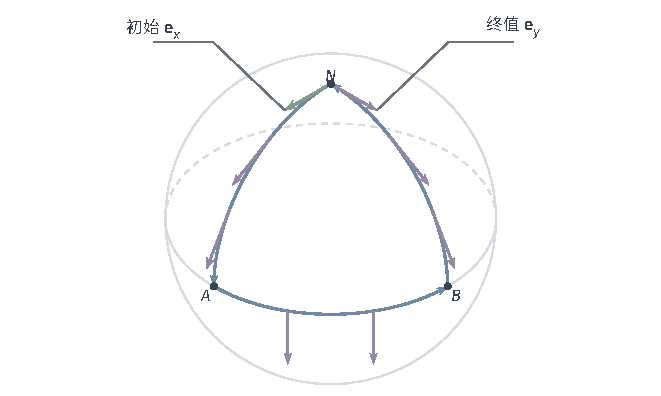
\includegraphics[width=112.0mm]{figures/01-mathematical-preliminaries-upper/02-linear-algebra-and-geometry/tikz/geometry-sphere-parallel-transport/figure.pdf}
  \caption{单位球面上沿$N\to A\to B\to N$的平行移动。
 蓝色为给定的三条大圆弧，紫箭头为例~\ref{ex:geometry-sphere-parallel-transport}
 中逐段计算的切向量。沿路协变导数为零，返回$N$后的方向却由初始箭头
 $\bm e_x$变为紫色终值箭头$\bm e_y$。
 箭头在三维中等长，投影到纸面后的长度可以不同。图为解析教学示例。}
 \label{fig:geometry-sphere-parallel-transport}
\end{figure}

这里的变换由路径和联络决定，不是任意选一个旋转来对齐环境向量。
前文群作用规定的是输入在指定变换下的响应；平行移动规定的是沿几何路径的方向比较，
即使二者有时都用矩阵表示，也不能据此互换。


球面闭路例子已经表明，搬运结果可以依赖路线。
为检测一个点附近的这种差异，可以比较沿两个方向先后求协变导数的结果。
方向场本身未必可交换，必须扣除$[\bm U,\bm V]$造成的变化，
剩下的才是联络对局部路径差异的响应。
这里有三个方向的不同职责：$\bm U,\bm V$指定小回路的两个方向，
另一个切向量$\bm W$是沿路搬运的箭头。给定前两个方向后，曲率作用在$\bm W$上，
检测绕路带来的方向变化；$\bm W$不必等于路径的前进速度。

\begin{definition}[Riemann曲率]
\label{def:geometry-riemann-curvature}
本章取曲率符号约定
\begin{equation}
 R(\bm U,\bm V)\bm W
 =\nabla_{\bm U}\nabla_{\bm V}\bm W
  -\nabla_{\bm V}\nabla_{\bm U}\bm W
  -\nabla_{[\bm U,\bm V]}\bm W.
 \label{eq:geometry-riemann-curvature}
\end{equation}
Levi--Civita联络的这个算子称为\term{Riemann曲率}（Riemann curvature）。
在点$\bm p$处，其值只依赖$\bm U,\bm V,\bm W$在该点的值，
而不依赖它们在附近的具体延拓。
\end{definition}
最后一项消掉方向场选择带来的导数项，使$R$成为按点定义的张量，即对点处方向多线性且不依赖坐标的对象。
例如在$\bm V$前乘光滑函数时，前两项会出现关于该函数的导数，
第三项恰好抵消它们。比较小闭路平行移动与恒等映射时，以闭路面积为尺度的
首项由$R(\bm u,\bm v)$控制；这个首项也可能为零，具体正负随绕行方向约定改变。
有限大闭路的总效应不能简单用某一点的曲率乘面积代替。

曲率算子仍含多个方向。选定一个二维切平面，可以用它给出一个标量曲率，
比较该平面内的局部几何。
\begin{definition}[截面曲率]
\label{def:geometry-sectional-curvature}
若$\bm u,\bm v\in T_{\bm p}\mathcal M$线性无关，
定义它们张成平面的\term{截面曲率}（sectional curvature）为
\begin{equation}
 K_{\bm p}(\bm u,\bm v)
 =\frac{g(R(\bm u,\bm v)\bm v,\bm u)}
 {g(\bm u,\bm u)g(\bm v,\bm v)-g(\bm u,\bm v)^2}.
 \label{eq:geometry-sectional-curvature}
\end{equation}
分母是该平行四边形的平方面积，正定性保证它为正。
\end{definition}
更换同一平面的基不改变比值。二维流形每点只有整个切平面这个选择，
所得量就是Gauss曲率；一维流形没有二维切平面，不能给圆硬套一个截面曲率数值。
一维Riemann曲率张量恒为零。

平面采用欧氏度量时，直角坐标中的联络系数为零，故$R=0$。
半径$R_0$的圆柱取局部参数
$(s,z)\mapsto(R_0\cos(s/R_0),R_0\sin(s/R_0),z)$，
诱导度量为$\mathrm ds^2+\mathrm dz^2$，
所以局部联络系数和内在曲率同样为零。
圆柱在环境中明显弯曲，却可以局部无伸缩地展开成平面；
把圆柱卷起来改变的是嵌入形状，不是这个局部度量。

半径$R_0$的球面则不同。对切向场，微分
$\langle\bm V,\bm p\rangle=0$给出
$\langle\mathrm d\bm V(\bm U),\bm p\rangle=-\langle\bm V,\bm U\rangle$，
因此
\[
 \nabla_{\bm U}\bm V
 =\mathrm d\bm V(\bm U)+\frac{g(\bm U,\bm V)}{R_0^2}\bm p.
\]
将其代入曲率定义，环境二阶导数与交换子相消；
再投影时，法向系数的导数被消去，而$\mathrm d\bm p(\bm U)=\bm U$留下
\[
 R(\bm U,\bm V)\bm W
 =\frac1{R_0^2}\bigl(g(\bm V,\bm W)\bm U-g(\bm U,\bm W)\bm V\bigr).
\]
代入式~\eqref{eq:geometry-sectional-curvature}便得任意截面
$K=1/R_0^2>0$。这也核对了本章曲率符号：球面的曲率为正。

在图~\ref{fig:geometry-sphere-parallel-transport}所用的单位球面北极
$N=(0,0,1)^\top$，取正交单位切向量$\bm u=\bm e_x$、$\bm v=\bm e_y$。
若被搬运的箭头取$\bm W=\bm v$，上式具体给出
\[
 R(\bm u,\bm v)\bm v=\bm u,\qquad
 K_N(\bm u,\bm v)=
 \frac{g(\bm u,\bm u)}{1\cdot1-0^2}=1.
\]
分子读出曲率作用后沿$\bm u$的分量，分母消去所选两方向围成的面积平方的尺度。
这里计算的是北极附近一个截面的局部曲率；前面的三段球面图则展示有限闭路的最终搬运。
缩小回路后观察方向变化的首项，才把这种沿路变化与局部曲率联系起来。

第\ref{sec:geometry-sampled-local-linearization}节将估计切平面；其法向误差需要与内在曲率区分。圆的一维方向沿环境空间转动，
产生二阶法向偏离，但其内在Riemann曲率为零；
圆柱也有法向弯曲而内在平坦。二维开带本来就是平面的开集，
式~\eqref{eq:geometry-strip-metric}虽有随位置变化的系数，内在曲率仍为零。
这些例子说明，法向二阶误差和Christoffel系数都不能单独作为内在非零曲率的证据。
局部曲率也不替代拓扑：平面与圆柱局部同样平坦，整体的环却不同；
局部零曲率本身不保证任意全局闭路上的搬运都平凡。

\subsection{对象的位置更新}
\label{sec:geometry-position-updates}
\label{sec:geometry-geodesic-motion-minimization}

\label{sec:geometry-geodesic-motion}

给定当前位置和一个切向步，直接沿环境直线前进通常会离开流形。
让速度沿自身路径平行移动，就能在保持初始速度大小的同时产生流形内的新位置。

\begin{definition}[测地线]
\label{def:geometry-geodesic}
相对于Riemann流形的Levi--Civita联络，采用仿射参数的曲线$\gamma$若满足
\[
 \frac{D\dot\gamma}{\mathrm dt}=\bm0,
\]
称为\term{测地线}（geodesic）。
\end{definition}
它没有切向加速度，速度沿自身路径作平行移动。
度量相容进一步给出
$\frac{\mathrm d}{\mathrm dt}\lVert\dot\gamma\rVert_g^2
=2g(D\dot\gamma/\mathrm dt,\dot\gamma)=0$，因此速度大小恒定。
环境加速度仍可非零，例如球面大圆需要法向加速度才能留在球面。

“仿射参数”说明换元$t=ar+b$、$a\neq0$保留这个方程。
一般换元则产生
\[
 \frac{D}{\mathrm dr}\frac{\mathrm d\gamma}{\mathrm dr}
 =(\tau'(r))^2\frac{D\dot\gamma}{\mathrm dt}
   +\tau''(r)\dot\gamma.
\]
非匀速参数化可以描出相同几何轨迹，却不再满足零协变加速度。
因此不能把路径长度的任意重参数化不变性照搬到这个运动方程。

要在坐标中求解，先用式~\eqref{eq:geometry-koszul-formula}取
$\bm U=\partial_i,\bm V=\partial_j,\bm W=\partial_\ell$。
坐标方向交换子为零，于是
\[
 2\sum_k g_{k,\ell}\Gamma^k_{i,j}
 =\partial_i g_{j,\ell}+\partial_j g_{i,\ell}-\partial_\ell g_{i,j}.
\]
乘逆度量便得到Christoffel符号
\begin{equation}
 \Gamma^k_{i,j}
 =\frac12\sum_{\ell=1}^d g^{k,\ell}
  \left(\frac{\partial g_{\ell,j}}{\partial z^i}
       +\frac{\partial g_{i,\ell}}{\partial z^j}
       -\frac{\partial g_{i,j}}{\partial z^\ell}\right),
 \qquad [g^{i,j}]=\bm G^{-1}.
 \label{eq:geometry-christoffel-symbols}
\end{equation}
将$\bm V=\dot\gamma=\sum_j\dot z^j\partial_j$代入
式~\eqref{eq:geometry-covariant-derivative-along-path}，测地条件成为
\begin{equation}
 \ddot z^k+\sum_{i,j=1}^d
 \Gamma^k_{i,j}(\bm z)\dot z^i\dot z^j=0.
 \label{eq:geometry-geodesic-equation}
\end{equation}
要判断这组系数是否表示点处的几何对象，需要区分几何张量与一张普通分量表。
这里的几何张量（geometric tensor）是点处、与坐标无关的多线性对象；
换基只对它的各个输入和输出作线性变换。因此，零分量表换基后仍为零。
Christoffel符号不满足这一规律。以正半轴的欧氏度量为例，
在坐标$x>0$中有$g_{x,x}=1$、$\Gamma^x_{x,x}=0$；
改用$x=e^u$后，$g_{u,u}=e^{2u}$，式~\eqref{eq:geometry-christoffel-symbols}给出
\[
 \Gamma^u_{u,u}=\frac12 e^{-2u}\frac{\mathrm d}{\mathrm du}e^{2u}=1.
\]
所以Christoffel符号是联络的坐标系数，不是张量。
基向量的变化与这些系数共同组成协变加速度，后者及所得曲线仍是几何对象。

光滑系数使这个二阶方程在给定
$\gamma(0)=\bm p$、$\dot\gamma(0)=\bm v$后具有局部唯一解，
并光滑依赖初值。这里“局部”同时限制时间和坐标覆盖范围；
可以换图延拓，但若路径有限时间离开流形，延拓就会失败。
开单位球内的欧氏直线从原点出发，以速度$2\bm e_1$前进，
在$t=1/2$时便到达不属于该流形的边界，不能默认解存在至$t=1$。

\begin{definition}[指数映射]
\label{def:geometry-exponential-map}
对给定$\bm p$，若初速度$\bm v$的测地线$\gamma_{\bm v}$存在至$t=1$，
定义
\[
 \operatorname{Exp}_{\bm p}(\bm v)=\gamma_{\bm v}(1).
\]
它称为$\bm p$处的\term{指数映射}（exponential map），
其定义域至少包含$T_{\bm p}\mathcal M$中零向量的一个邻域。
\end{definition}
初速度缩放对应时间缩放：
$\operatorname{Exp}_{\bm p}(t\bm v)=\gamma_{\bm v}(t)$，只在两边均有定义时使用。
因而$\operatorname{Exp}_{\bm p}(\bm0)=\bm p$且
$\mathrm d(\operatorname{Exp}_{\bm p})_{\bm0}=\operatorname{id}_{T_{\bm p}\mathcal M}$。
逆函数定理保证在足够小邻域中它是微分同胚；
这为用切向量表示附近点提供了一种局部方式，不保证全局一一对应。

单位球面上，$\bm v\perp\bm p$、$r=\lVert\bm v\rVert_2$时，
\begin{equation}
 \operatorname{Exp}_{\bm p}(\bm v)
 =\cos r\,\bm p+\frac{\sin r}{r}\bm v,
 \label{eq:geometry-sphere-exponential}
\end{equation}
$r=0$时按连续延拓取$\bm p$。
对应曲线$\gamma(t)=\cos(tr)\bm p+\sin(tr)\bm v/r$
满足$\lVert\gamma(t)\rVert_2=1$、初速度为$\bm v$，
且$\ddot\gamma=-r^2\gamma$为纯法向，所以确实解测地线方程。
所有方向上长度为$\pi$的初速度都到达对跖点$-\bm p$；
即使映射处处有定义，也未必全局单射。


切向量$\bm v$给出可行的瞬时方向，有限位移$\bm p+\bm v$却通常离开流形。
指数映射给出一种更新，但求解精确测地线可能昂贵。
如果只需保证一阶变化正确，可以使用更易计算的局部返回映射。

\begin{definition}[回缩]
\label{def:geometry-retraction}
对每个$\bm p$，在$T_{\bm p}\mathcal M$的零向量邻域中给定
$\mathcal R_{\bm p}(\bm v)\in\mathcal M$，并使其光滑依赖$(\bm p,\bm v)$。
若
\[
 \mathcal R_{\bm p}(\bm0)=\bm p,\qquad
 \mathrm d(\mathcal R_{\bm p})_{\bm0}[\bm v]=\bm v,
\]
则称这一族映射为\term{回缩}（retraction）。
\end{definition}
第一项保留起点，第二项保留初速度。它不要求沿$t\mapsto\mathcal R_{\bm p}(t\bm v)$
作精确测地运动，也不要求任意大步长都在定义域中。
指数映射是一种局部回缩，其他回缩可有不同的高阶误差。


这些映射接收当前位置与一个小切向步，输出新位置。
它们只规定一步怎样保持可行；怎样选择方向、步长以及整个序列是否收敛，是后面的求解与收敛问题。

\subsection{区域的体积计算}
\label{sec:geometry-riemannian-volume}

要比较区域的大小，路径的一维长度还不够，需要给小区域规定体积。
坐标切基围成的微小平行体，其平方体积是Gram行列式$\det\bm G$，
因此几何体积元为
\begin{equation}
 \mathrm dV_g=\sqrt{\det\bm G(\bm z)}\,\mathrm d\bm z.
 \label{eq:geometry-riemannian-volume}
\end{equation}
这是由度量产生的测度密度，不要求先为流形选定全局朝向。
一维时给出长度，二维时给出面积。

坐标变换$\bm z=\psi(\bm v)$下，
$\det\widetilde{\bm G}=(\det\bm A)^2\det\bm G$，所以
\[
 \sqrt{\det\widetilde{\bm G}}\,\mathrm d\bm v
 =\sqrt{\det\bm G(\psi(\bm v))}\,|\det\bm A|\,\mathrm d\bm v.
\]
它正是多元积分换元中的Jacobian因子，故对可积函数所得积分不依赖坐标。
跨图时必须避免把重叠区域重复计数，可分割成可测片段分别积分；
光滑计算也可使用从属于图册、和为$1$的局部权重来拼接。

点带中$\sqrt{\det\bm G}=1+u/R>0$，
小盒$\mathrm ds\,\mathrm du$在外侧对应较大面积。
中心线限制为$u=0$后的一维体积元是$\mathrm ds$，不是把二维面积直接代入。
若样本相对几何体积有密度$q$，其分布测度是$q\,\mathrm dV_g$；
当样本独立同分布地取自这个测度，且$\int|f|q\,\mathrm dV_g<\infty$时，
简单样本平均的期望是$\int fq\,\mathrm dV_g$；大数定律还保证它收敛到这个
加权积分。它并非自动近似$\int f\,\mathrm dV_g$。
几何体积与采样权重的差别将在离散平滑目标中再次出现。

当前开带无流形边界，但不是紧集。需要边界积分时，将另取有分片光滑边界的
截断闭域，并声明函数在边界的行为；不能只因图上画有虚线就把它当作同一个积分问题。

\section{方程与优化}
\label{sec:geometry-equations-optimization}

前面的运算可以计算已知点或方向的响应，现在用它们求未知对象。
给定两两距离时，未知量是一组坐标；给定位置与速度时，未知量是一条运动轨迹。
若改为给定两个端点，还需比较允许路线的长度。最后在流形中寻找目标值最小的点，
其可行更新将调用微分、度量和回缩。

\subsection{距离信息下的坐标重构}
\label{sec:geometry-distance-coordinate-embedding}

设只知道$n$个点之间的距离，能否给它们安排欧氏坐标，并精确保留这些距离？
先从反方向计算。将$\bm y_1,\ldots,\bm y_n\in\mathbb R^d$按行组成
$\bm Y\in\mathbb R^{n\times d}$。定义~\ref{def:linear-algebra-gram-matrix}中的
\term{Gram矩阵}$\bm B=\bm Y\bm Y^\top$记录两两内积，平方距离则为
\begin{equation}
  \delta_{i,j}=\lVert\bm y_i-\bm y_j\rVert_2^2
  =b_{i,i}+b_{j,j}-2b_{i,j}.
  \label{eq:geometry-distance-from-gram}
\end{equation}
距离不记录原点：将全部点平移同一个向量，差向量不变，内积却会改变。
因此从距离恢复内积前，需要先固定平移自由度。

把点云均值选为原点。令$\bm1\in\mathbb R^n$为全一向量，定义
\begin{equation}
  \bm J=\bm I_n-\frac1n\bm1\bm1^\top.
  \label{eq:geometry-centering-matrix}
\end{equation}
它满足$\bm J^\top=\bm J$、$\bm J^2=\bm J$和$\bm J\bm1=\bm0$；
$\bm J\bm Y$从每行减去样本均值。若$\bm\Delta=[\delta_{i,j}]$，
式~\eqref{eq:geometry-distance-from-gram}写成
\[
  \bm\Delta=\operatorname{diag}(\bm B)\bm1^\top
  +\bm1\operatorname{diag}(\bm B)^\top-2\bm B.
\]
左右各乘$\bm J$，前两项消失。对于已中心化的坐标，
$\bm J\bm Y=\bm Y$，于是
\begin{equation}
  \bm B=-\frac12\bm J\bm\Delta\bm J.
  \label{eq:geometry-double-centering}
\end{equation}
这称为\term{双重中心化}（double centering）：在两个点索引上消去均值项，
把平方距离转成以点云中心为原点的内积。此时尚未作低维投影。

任何真实坐标产生的Gram矩阵都半正定，因为
$\bm c^\top\bm B\bm c=\lVert\bm Y^\top\bm c\rVert_2^2\geq0$。
要证明这个条件也足够，需要排除双重中心化过程中丢失了某种非零距离差。

\begin{lemma}[双重中心化核的形式]
\label{lem:geometry-double-centering-kernel}
若对称矩阵$\bm H\in\mathbb R^{n\times n}$满足$\bm J\bm H\bm J=\bm0$，
则存在$\bm a\in\mathbb R^n$使
$\bm H=\bm1\bm a^\top+\bm a\bm1^\top$。
若另有$h_{i,i}=0$对全部$i$成立，则$\bm H=\bm0$。
\end{lemma}
\begin{proof}
令$\bm m=\bm H\bm1/n$、$\mu=\bm1^\top\bm H\bm1/n^2$。展开假设得到
\[
  \bm H=\bm1\bm m^\top+\bm m\bm1^\top-\mu\bm1\bm1^\top.
\]
取$\bm a=\bm m-(\mu/2)\bm1$即得所需形式。其对角元为$h_{i,i}=2a_i$，
故零对角条件迫使每个$a_i=0$，进而$\bm H=\bm0$。
\end{proof}

\begin{theorem}[有限距离的欧氏坐标重构]
\label{thm:geometry-euclidean-distance-embedding}
设$\bm\Delta\in\mathbb R^{n\times n}$对称且对角元为零，并令
$\bm B=-\bm J\bm\Delta\bm J/2$。矩阵$\bm\Delta$是某组欧氏点的平方距离矩阵，
当且仅当$\bm B$半正定。精确保留全部距离所需的最小欧氏维数为
$r=\operatorname{rank}(\bm B)$。
\end{theorem}
\begin{proof}
若已有欧氏点，先中心化，式~\eqref{eq:geometry-double-centering}便给出
$\bm B=\bm Y\bm Y^\top$，所以$\bm B$半正定。

反过来，半正定性和谱定理给出紧谱分解
$\bm B=\bm Q_r\bm\Lambda_r\bm Q_r^\top$，其中$\bm\Lambda_r$含$r$个正特征值。
取
\begin{equation}
  \bm Y=\bm Q_r\bm\Lambda_r^{1/2},
  \label{eq:geometry-classical-scaling-coordinates}
\end{equation}
则$\bm Y\bm Y^\top=\bm B$。又因$\bm B\bm1=\bm0$，
$\lVert\bm Y^\top\bm1\rVert_2^2=\bm1^\top\bm B\bm1=0$，坐标已中心化。
用式~\eqref{eq:geometry-distance-from-gram}从$\bm B$生成$\bm\Delta'$。
$\bm\Delta'$与$\bm\Delta$的双重中心化均为$\bm B$，两者之差对称、
对角为零且双重中心化为零。前一引理遂给出$\bm\Delta'=\bm\Delta$。

任意$\mathbb R^k$中的坐标矩阵所产生的Gram矩阵秩至多为$k$，
因此精确重构要求$k\geq r$；上述构造又在$k=r$时达到要求。
$r=0$时全部点重合，可视为嵌入零维空间。
\end{proof}

这个判据是经典尺度分析的代数核心。$\bm B$有负特征值时，输入关系不能被精确实现为
欧氏平方距离。逐对测量的距离误差可能造成负谱；直接由一组带噪坐标精确计算的距离
却仍来自欧氏点，其Gram矩阵不会仅因坐标带噪而失去半正定性。后者重构的是观测点，
不是噪声发生前的潜在点。

距离保留了相对位置，却不能确定绝对位置、朝向或手性。对正交矩阵
$\bm Q\in\mathbb R^{r\times r}$和平移$\bm a$，令
$\widetilde{\bm y}_i=\bm Q\bm y_i+\bm a$，则
\[
 \lVert\widetilde{\bm y}_i-\widetilde{\bm y}_j\rVert_2
 =\lVert\bm Q(\bm y_i-\bm y_j)\rVert_2
 =\lVert\bm y_i-\bm y_j\rVert_2.
\]
正交变换既含旋转，也含反射。中心化只消去平移，不能选择唯一朝向。

对于中心化的最小维坐标，这也是全部不确定性。设
$\bm Y,\widetilde{\bm Y}\in\mathbb R^{n\times r}$均列满秩并产生相同距离，
则双重中心化给出相同$\bm B$。它们的列空间都等于$\bm B$的值域。
对$\bm B=\bm Q_r\bm\Lambda_r\bm Q_r^\top$定义
$\bm M=\bm\Lambda_r^{-1/2}\bm Q_r^\top\bm Y$，可得
\[
 \bm Y=\bm Q_r\bm\Lambda_r^{1/2}\bm M,\qquad
 \bm M\bm M^\top
 =\bm\Lambda_r^{-1/2}\bm Q_r^\top\bm B\bm Q_r
   \bm\Lambda_r^{-1/2}=\bm I_r.
\]
方阵$\bm M$因而正交。写$\bm M=\bm U^\top$，对另一组坐标同样得到
$\widetilde{\bm Y}=\bm Q_r\bm\Lambda_r^{1/2}\widetilde{\bm U}^\top$，
于是$\widetilde{\bm Y}=\bm Y\bm U\widetilde{\bm U}^\top$。
重复特征值允许坐标轴在对应子空间内旋转；更高维实现的额外方向不含点云信息，
两组点仍在各自张成空间之间具有保距正交对应。

\begin{example}[三个点能否放在一条直线上]
\label{ex:geometry-three-point-embedding}
取$\bm y_1=(-1,0)^\top$、$\bm y_2=(0,1)^\top$、
$\bm y_3=(1,0)^\top$，其均值是$(0,1/3)^\top$。平方距离与中心化结果为
\[
 \bm\Delta=\begin{bmatrix}0&2&4\\2&0&2\\4&2&0\end{bmatrix},
\]
\begin{equation}
 -\frac12\bm J\bm\Delta\bm J
 =\begin{bmatrix}
  10/9&-2/9&-8/9\\
  -2/9&4/9&-2/9\\
  -8/9&-2/9&10/9
 \end{bmatrix}.
 \label{eq:geometry-three-point-centered-gram}
\end{equation}
正特征值为$2$和$2/3$，所以精确重构需要二维。
若只保留特征值$2$对应的水平方向，端点间距离仍为$2$，
顶点到两端的距离却从$\sqrt2$变成$1$；这是一种近似，不是另一份精确坐标。
\end{example}

这里必须区分谱近似的目标。若$\bm B$半正定，保留最大$k<r$个特征值时，
定理~\ref{thm:matrix-analysis-best-low-rank}保证Gram矩阵的Frobenius误差最小，
平方误差为$\sum_{j>k}\lambda_j^2$。在一组给定中心化坐标上作对应PCA投影，
坐标平方重构误差则为$\sum_{j>k}\lambda_j$。若原距离为
$d_{i,j}=\sqrt{\delta_{i,j}}$，近似坐标为$\widetilde{\bm y}_i$，
还可以直接比较逐对距离，例如把距离应力（distance stress）取为
\[
 \sum_{i<j}
 \bigl(\lVert\widetilde{\bm y}_i-\widetilde{\bm y}_j\rVert_2-d_{i,j}\bigr)^2.
\]
它比较距离，前两种误差分别比较内积和坐标，因此优化目标不同。
最大相对距离误差则比较
\[
 \max_{\substack{i<j\\d_{i,j}>0}}
 \frac{\bigl|\lVert\widetilde{\bm y}_i-\widetilde{\bm y}_j\rVert_2-d_{i,j}\bigr|}
 {d_{i,j}}.
\]
全体点重合时不使用这个比值准则。对含负谱的$\bm B$，保留最大的至多$k$个正特征值给出
半正定秩至多$k$约束下的Frobenius近似；舍弃负谱的大小仍须与测量误差比较。

有限坐标重构也不证明潜在集合是一张光滑曲面。即使点落在圆上，输入欧氏距离记录的仍是
弦长，不能把保弦长的坐标自动解释为沿圆排列的一维坐标。要表达连续对象的自由度，
必须另行给出局部模型。

\subsection{初值条件下的测地轨迹求解}
\label{sec:geometry-geodesic-initial-value}

给定$\gamma(0)=\bm p$与$\dot\gamma(0)=\bm v$，求满足
式~\eqref{eq:geometry-geodesic-equation}的轨迹。把二阶方程改写为$(z,\dot z)$的一阶系统，
局部光滑系数保证解在初值附近存在唯一。这里固定的是位置与速度，不是两个端点。
在重叠坐标图中，已有解与换图后的解由唯一性拼接，从而得到最大延拓区间。
只要位置与速度留在一组系数受控的紧区域内，就可继续局部求解；
流形缺口或无界离开会阻止这个过程。

完整单位球面上，取$\bm p\in S^{D-1}$、$\bm v\perp\bm p$，则
$\gamma(t)=\cos(t\lVert\bm v\rVert_2)\bm p
+\sin(t\lVert\bm v\rVert_2)\bm v/\lVert\bm v\rVert_2$
对全部$t$存在，$\bm v=\bm0$时取恒定轨迹。开球的直线却可能有限时间到达缺失边界。
第\ref{sec:geometry-endpoint-minimizing-path}节的完备性条件将给出全局延拓保证，
但初值的唯一性并不保证指定端点之间只有一条路径。

\subsection{端点约束下的最短路径求解}
\label{sec:geometry-endpoint-minimizing-path}

现在给定$\bm p,\bm q$，要求找到达到
式~\eqref{eq:geometry-geodesic-distance}下确界的路径。
其与测地方程的联系可通过路径能量建立。固定时间区间$[a,b]$，定义
\[
 E(\gamma)=\frac12\int_a^b\lVert\dot\gamma\rVert_g^2\,\mathrm dt.
\]
由Cauchy--Schwarz不等式，
$L_g(\gamma)^2\leq2(b-a)E(\gamma)$，等号恰对应几乎处处恒定的速度大小。
因此对可作匀速参数化的非退化路径，最小化长度可联系到固定时间的能量最小化；
能量本身却不具有长度那样的任意重参数化不变性。

在局部坐标中，Lagrange函数为
$\mathscr L(\bm z,\dot{\bm z})=\frac12\sum_{i,j}g_{i,j}(\bm z)\dot z^i\dot z^j$。
取光滑扰动$\bm h$，满足$\bm h(a)=\bm h(b)=\bm0$，并令
$\bm z_\varepsilon(t)=\bm z(t)+\varepsilon\bm h(t)$。
取足够小的$\varepsilon$使路径仍在坐标域内。
若$\varphi$为当前坐标的参数化，一阶变分就是把整条路径沿这个方向改变后，
能量关于扰动幅度的导数：
\[
 \delta E[\bm h]
 =\left.\frac{\mathrm d}{\mathrm d\varepsilon}
 E(\varphi\circ\bm z_\varepsilon)\right|_{\varepsilon=0}.
\]
对积分求导并分部积分，得到
\[
 \delta E[\bm h]
 =\int_a^b\sum_k\left(
 \frac{\partial\mathscr L}{\partial z^k}
 -\frac{\mathrm d}{\mathrm dt}
     \frac{\partial\mathscr L}{\partial\dot z^k}\right)h^k\,\mathrm dt.
\]
边界项因固定端点消失。驻定要求任意这样的$\bm h$都使变分为零，
因此括号中每个系数都必须为零：若某个连续系数在一点非零，
就在它保持同号的小邻域内取一个同号、光滑且在邻域外为零的扰动，
相应积分便不为零，产生矛盾。计算括号中的两个偏导得
\[
 \begin{aligned}
 \frac{\partial\mathscr L}{\partial z^k}
   &=\frac12\sum_{i,j}\partial_k g_{i,j}\dot z^i\dot z^j,\\
 \frac{\mathrm d}{\mathrm dt}
    \frac{\partial\mathscr L}{\partial\dot z^k}
   &=\sum_j g_{k,j}\ddot z^j+
     \sum_{i,j}\partial_i g_{k,j}\dot z^i\dot z^j.
 \end{aligned}
\]
对第二行的速度乘积对称化后，Euler--Lagrange方程为
\[
 \sum_jg_{k,j}\ddot z^j+
 \frac12\sum_{i,j}
  (\partial_i g_{k,j}+\partial_j g_{k,i}-\partial_k g_{i,j})
  \dot z^i\dot z^j=0.
\]
乘$\bm G^{-1}$即得式~\eqref{eq:geometry-geodesic-equation}。
跨图路径可对各段内支撑的扰动分别推导，得到相同几何方程。
这说明光滑匀速最短路必为测地线，不说明每个能量驻点都是最短路。

指数映射给出描述这些局部路径的区域。取零切向量附近的小开集$V$，
要求$\bm v\in V$时$t\bm v\in V$对$0\leq t\leq1$成立，
且$\operatorname{Exp}_{\bm p}$在$V$上为微分同胚。
它的像称为$\bm p$的正规邻域（normal neighborhood），
其中每个点都用一个初速度表示，径向路径对应$t\bm v$。
标准局部最短性结论保证可以把这个区域取到足够小，
使径向测地线段在邻域内达到端点间的最短长度。
还可进一步选择凸正规邻域（convex normal neighborhood），
让其中任意两点由唯一的邻域内最短测地线连接，整条线段留在该邻域中。
这里“凸”指测地线连接的性质，不是要求环境中的欧氏直线段留在区域内。
这项结论利用指数映射和径向、横向变化的正交性，不是只凭微分方程存在唯一性得到的。
离开这种局部范围后，其他路线可能更短。
若一段测地线达到$d_g$，称为\term{长度最短测地线}（length-minimizing geodesic）。

完整单位圆上，从$(1,0)^\top$到$(0,-1)^\top$的逆时针弧长为$3\pi/2$，
顺时针弧长为$\pi/2$。两条匀速圆弧都满足零协变加速度，
只有后者达到距离。相同的初值局部运动规则不承担全局路线比较。
割点研究从某点出发的测地线何时失去最短性，
共轭点涉及相邻测地线的聚焦与变分退化；这些进一步判据不在本章展开，
不能据术语本身判定一条路径最短。

\begin{theorem}[Hopf--Rinow定理的最短路存在性结论]
\label{thm:geometry-hopf-rinow-existence}
设$(\mathcal M,g)$为有限维、连通、无边界的光滑Riemann流形。
若它关于$d_g$完备，则任意两点之间存在长度最短测地线。
此时任意初速度的测地运动也可以延拓到所有实数时间。
\end{theorem}
这里引用这一定理的存在性结论，不展开完整等价条件及证明。
完备性是每个$d_g$-Cauchy序列都在$\mathcal M$内收敛；
它限制了路径是否能在有限长度内跑到空间缺口。
结论保证存在而不保证唯一：球面的对跖点之间有多条最短大圆弧，
指数映射仍不是全局单射。紧致无边界的Riemann流形满足这里的完备性条件。

穿孔平面给出省略完备性的反例。用欧氏诱导度量连接
$(-1,0)^\top$和$(1,0)^\top$，
沿横轴走到$(-\varepsilon,0)^\top$，绕半径$\varepsilon$的半圆，
再沿横轴到终点，长度为
\[
 (1-\varepsilon)+\pi\varepsilon+(1-\varepsilon)
 =2+(\pi-2)\varepsilon\longrightarrow2.
\]
环境距离给出下界$2$，所以$d_g=2$。
长度等于端点欧氏距离的路径只能沿连接线段前进，该线段经过被删去的原点，
故没有允许路径达到下确界。这里仍有局部测地解，却没有这两个端点的最短路。

\subsection{流形约束下的点优化}
\label{sec:geometry-point-optimization}
\label{sec:geometry-manifold-optimization}
\label{sec:geometry-point-optimality}

考虑$\min_{\bm p\in\mathcal M}f(\bm p)$，其中$f$为至少二阶连续可微的实函数。
流形约束已经包含在可行域中。普通偏导给出坐标变化，
但实际可行的一阶变化属于$T_{\bm p}\mathcal M$；
有限步更新还必须从切空间返回流形。


在选择迭代方法以前，先检查这个最小值是否存在。若非空流形$\mathcal M$紧致且$f$连续，
极小值定理保证全局最小值存在；非紧空间上可用紧的非空下水平集等条件替代，
不能只凭可微性保证存在。局部极小只和附近可行点比较，全局极小则和全部可行点比较。
以下最优性条件讨论无边界流形的点，不覆盖另加不等式所造成的活动边界。

第\ref{sec:geometry-tangent-maps}节已将微分$\mathrm df_{\bm p}$定义为对切向量的线性读取。
要从这个读取规则选出最陡方向，还需用度量把它表示成向量。
\begin{definition}[Riemann梯度]
\label{def:geometry-riemannian-gradient}
给定光滑函数$f$，点$\bm p$处的\term{Riemann梯度}（Riemannian gradient）
是由下式唯一确定的切向量$\operatorname{grad}f(\bm p)$：
\begin{equation}
 g_{\bm p}(\operatorname{grad}f,\bm v)=\mathrm df_{\bm p}(\bm v)
 \qquad(\bm v\in T_{\bm p}\mathcal M)
 \label{eq:geometry-riemannian-gradient-definition}
\end{equation}
\end{definition}
有限维内积的正定性保证存在唯一的表示向量。
微分由$f$决定，梯度还依赖度量；改变度量会改变最陡方向，但不改变微分是否为零。
在非驻点处，由Cauchy--Schwarz不等式，在$\lVert\bm v\rVert_g=1$的方向中，
$\mathrm df(\bm v)$最小为$-\lVert\operatorname{grad}f\rVert_g$，
并在负梯度的单位方向达到。驻点处各切向方向的一阶变化都为零。

设$\widehat f=f\circ\varphi$为坐标表达，为简洁把其偏导列表写作
\[
 \nabla_{\bm z}f=(\partial_1\widehat f,\ldots,\partial_d\widehat f)^\top.
\]
若梯度坐标为$\bm a$，则对所有坐标向量$\bm v$有
$\bm a^\top\bm G\bm v=\nabla_{\bm z}f^\top\bm v$，所以
\begin{equation}
 [\operatorname{grad}f]_{\bm z}=\bm G^{-1}\nabla_{\bm z}f.
 \label{eq:geometry-riemannian-gradient-coordinates}
\end{equation}
偏导列表表示余切向量，逆度量把它转为切向量；只有特定正交归一坐标中二者分量相同。
对欧氏诱导度量，若$f$有环境光滑延拓$\bar f$，则
$\operatorname{grad}f(\bm p)=\bm P_{\bm p}\nabla\bar f(\bm p)$，
因为投影不改变与任一切向量的内积。

梯度的一阶变化属于不同位置的切空间，不能直接求差后当作二阶信息。
联络给出所需的比较规则。
\begin{definition}[Riemann Hessian]
\label{def:geometry-riemannian-hessian}
在Levi--Civita联络下，定义\term{Riemann Hessian}（Riemannian Hessian）为线性算子
\[
 \operatorname{Hess}f(\bm p)[\bm v]
 =\nabla_{\bm v}\operatorname{grad}f
 \quad\text{从 }T_{\bm p}\mathcal M\text{ 到自身}.
\]
其双线性形式为
$\operatorname{Hess}f(\bm u,\bm v)
=g(\bm u,\operatorname{Hess}f[\bm v])$。
\end{definition}
度量相容和无挠使双线性形式对称。具体地，
\[
 g(\nabla_{\bm U}\operatorname{grad}f,\bm V)
 =\bm U(\bm V f)-(\nabla_{\bm U}\bm V)f;
\]
交换$\bm U,\bm V$后的差为
$[\bm U,\bm V]f-(\nabla_{\bm U}\bm V-\nabla_{\bm V}\bm U)f=0$。
在坐标中双线性形式的矩阵是
\begin{equation}
 B_{i,j}=\partial_i\partial_j\widehat f
             -\sum_k\Gamma^k_{i,j}\partial_k\widehat f,
 \qquad [\operatorname{Hess}f]_{\bm z}=\bm G^{-1}\bm B.
 \label{eq:geometry-hessian-coordinates}
\end{equation}
矩阵$\bm B$对称；线性算子的坐标矩阵$\bm G^{-1}\bm B$一般不是普通转置意义的
对称矩阵，却相对于内积$\bm G$自伴。非驻点处不能省略联络修正项。

沿任意$C^2$曲线，对$f(\gamma(t))$再求一次导数可得
\begin{equation}
 \frac{\mathrm d^2}{\mathrm dt^2}f(\gamma(t))
 =g(\operatorname{Hess}f[\dot\gamma],\dot\gamma)
   +g(\operatorname{grad}f,D\dot\gamma/\mathrm dt).
 \label{eq:geometry-function-second-derivative}
\end{equation}
测地线上第二项为零。因此，在无边界的局部极小点$\bm p_*$，
任意初速度的测地线都给出一元局部极小，必要条件为
\[
 \operatorname{grad}f(\bm p_*)=\bm0,\qquad
 g(\operatorname{Hess}f(\bm p_*)[\bm v],\bm v)\geq0
 \quad\text{对所有 }\bm v.
\]
若梯度为零且Hessian正定，指数坐标中的二阶Taylor展开给出严格局部极小。
半正定只给必要性，仍需更高阶信息；梯度为零也可能是极大点或鞍点。

欧氏凸性不能不加条件地移到弯曲可行域，因为连接两点的环境线段未必可行。
一种替代条件是\term{测地凸性}（geodesic convexity）：
在一个任意两点都可由域内最短测地线连接的区域$\Omega$上，
若$f$沿每条这样的仿射参数测地线都是一元凸函数，就称其在该区域测地凸。
此时对从$\bm p$到$\bm q$的此类路径，一元凸性给出
$f(\bm q)\geq f(\bm p)+\mathrm df_{\bm p}(\dot\gamma(0))$
（参数区间取$[0,1]$）；故域内驻点是域内全局极小。
区域是否具有所需连接性质、函数是否满足沿路凸性，都须验证，
不能由“目标来自欧氏凸函数”自动推出。

\subsubsection{基于梯度与回缩的一阶求解}
\label{sec:geometry-riemannian-gradient-method}

用括号上标记录迭代步，梯度更新写成
\begin{equation}
 \bm p^{(k+1)}=\mathcal R_{\bm p^{(k)}}
       (-\alpha^{(k)}\operatorname{grad}f(\bm p^{(k)})).
 \label{eq:geometry-riemannian-gradient-step}
\end{equation}
回缩的一阶相容性保证，沿该搜索曲线在$\alpha=0$处
\[
 \frac{\mathrm d}{\mathrm d\alpha}
 f(\mathcal R_{\bm p}(-\alpha\operatorname{grad}f))
 \bigg|_{\alpha=0}=-\lVert\operatorname{grad}f\rVert_g^2.
\]
因此非驻点处足够小的正步长确实下降。可以在回缩定义域内回溯，检验
$f(\bm p^{(k+1)})\leq f(\bm p^{(k)})
-c\alpha^{(k)}\lVert\operatorname{grad}f(\bm p^{(k)})\rVert_g^2$，
其中$0<c<1$。这只是逐步下降机制；
若还要推出梯度范数趋零，通常需紧的下水平集、目标下界、
回缩拉回函数的统一局部光滑界和相应回溯规则。
非凸问题不能因此保证全局极小，梯度范数趋零也不等于迭代点必然收敛。

\begin{example}[球面上的归一化更新]
\label{ex:geometry-sphere-retraction}
单位球面上$\bm p^\top\bm v=0$，故
$\lVert\bm p+\bm v\rVert_2=\sqrt{1+\lVert\bm v\rVert_2^2}$。取
\begin{equation}
 \mathcal R_{\bm p}(\bm v)
 =\frac{\bm p+\bm v}{\sqrt{1+\lVert\bm v\rVert_2^2}}.
 \label{eq:geometry-sphere-retraction}
\end{equation}
结果始终在球面上，零点导数为$\bm v$，所以是回缩。
设$r=\lVert\bm v\rVert_2>0$，回缩终点与起点的夹角为$\arctan r$。
指数映射则沿同一大圆行进长度$r$；当$0<r<\pi$时，这也等于两个端点的夹角。
二者只在小步长下接近，不是同一更新。

例如$f(\bm p)=-\bm a^\top\bm p$、$\bm a\neq\bm0$，
有$\operatorname{grad}f=-\bm a+(\bm a^\top\bm p)\bm p$。
先将环境下降方向$\bm a$投影到当前切空间，得到$-\operatorname{grad}f$，
再由归一化回缩把切向步变成球面上的新点。
驻点为$\pm\bm a/\lVert\bm a\rVert_2$；
在切空间上$\operatorname{Hess}f[\bm v]=(\bm a^\top\bm p)\bm v$，
故正向驻点是严格极小，反向驻点是严格极大。
单独检验梯度为零无法区分二者。
\end{example}

图~\ref{fig:geometry-sphere-retraction}固定同一个切向步，比较指数映射和归一化回缩。
两种更新都可行，但沿大圆走过的角度不同。
\begin{figure}[htbp]
  \centering
  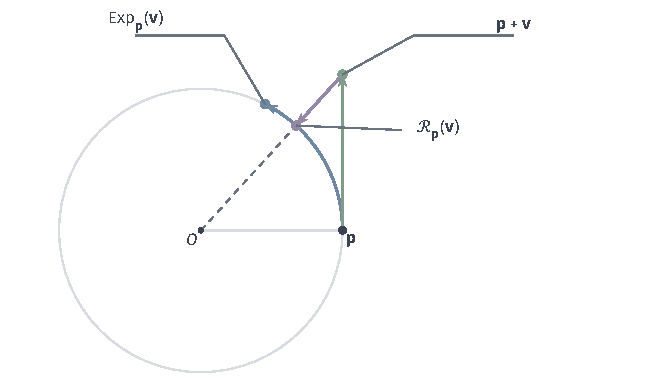
\includegraphics[width=112.0mm]{figures/01-mathematical-preliminaries-upper/02-linear-algebra-and-geometry/tikz/geometry-sphere-retraction/figure.pdf}
  \caption{单位圆截面中的切向步、指数映射与归一化回缩。
 取$\bm p=(1,0)^\top$、$\bm v=(0,1.1)^\top$。箭头为切向步，
 终点$\bm p+\bm v$位于圆外；紫色径向箭头将该点归一化为$\mathcal R_{\bm p}(\bm v)$。
 从起点方向计，蓝色指数更新转过$1.1$弧度，归一化回缩转过
 $\arctan(1.1)\approx0.833$弧度。两种更新关于步长的曲线在零步长处有相同初速度，
 但有限步位置不同。图为解析教学示例。}
 \label{fig:geometry-sphere-retraction}
\end{figure}
\FloatBarrier

\subsubsection{基于Newton与信赖域的二阶求解}
\label{sec:geometry-riemannian-newton-trust-region}

梯度只给局部下降方向，Hessian还能描述不同方向的二阶变化。
在当前点$\bm p$的切空间建立模型
\[
 m_{\bm p}(\bm\eta)=f(\bm p)
  +g(\operatorname{grad}f,\bm\eta)
  +\frac12g(\bm\eta,\operatorname{Hess}f[\bm\eta]).
\]
Newton方向解
$\operatorname{Hess}f[\bm\eta]=-\operatorname{grad}f$，
再用$\mathcal R_{\bm p}(\alpha\bm\eta)$更新。
取切空间正交归一基后，这是已有线性求解方法处理的对称系统；
一般坐标中可用式~\eqref{eq:geometry-hessian-coordinates}写成
$\bm B\bm\eta=-\nabla_{\bm z}f$。
Hessian奇异时方向可能不存在或不唯一，不定时Newton方向也可能不是下降方向。
局部快速收敛需要非退化解、足够光滑性、合适回缩和足够近的初始点，
不是二阶公式本身提供的全局保证。

信赖域方法限制模型适用范围，在$\lVert\bm\eta\rVert_g\leq\Delta$中近似最小化
$m_{\bm p}$。用实际下降与预测下降之比
\[
 \rho=\frac{f(\bm p)-f(\mathcal R_{\bm p}(\bm\eta))}
             {m_{\bm p}(\bm0)-m_{\bm p}(\bm\eta)}
\]
判断接受步和调整$\Delta$，只在分母为正时使用这个比值。
它允许利用负曲率方向，同时避免把远离当前点的模型误当成目标本身。
收敛结论仍需模型误差控制、子问题下降量及更新规则。

这里有一个二阶条件容易遗漏。令拉回目标
$\widehat f_{\bm p}(\bm\eta)=f(\mathcal R_{\bm p}(\bm\eta))$，
它定义在固定向量空间$T_{\bm p}\mathcal M$上。
回缩只保证其零点一阶导数等于$\mathrm df_{\bm p}$。
设$c(t)=\mathcal R_{\bm p}(t\bm\eta)$，由
式~\eqref{eq:geometry-function-second-derivative}，
\begin{equation}
 \frac{\mathrm d^2}{\mathrm dt^2}\widehat f_{\bm p}(t\bm\eta)
 \bigg|_{t=0}
 =g(\bm\eta,\operatorname{Hess}f[\bm\eta])
  +g(\operatorname{grad}f,D\dot c/\mathrm dt|_{t=0}).
 \label{eq:geometry-retraction-pullback-hessian}
\end{equation}
若回缩对所有$\bm\eta$均满足$D\dot c/\mathrm dt|_0=\bm0$，
称为二阶回缩（second-order retraction）。此时，或当前点已经驻定时，额外项才必定消失，
拉回目标的零点Hessian才与Riemann Hessian一致。
指数映射满足该条件；球面归一化回缩也满足，因为
$c''(0)=-\lVert\bm\eta\rVert_2^2\bm p$为纯法向。
对任意一阶回缩直接作二阶等同则不成立，
必须修正模型或另外证明所用模型满足算法的误差要求。
这些模型条件及一阶、二阶算法的收敛分析可参见Boumal的教材\scite{math-boumal2023optimization}。

若算法还复用前一步动量或搜索方向，它们位于旧切空间，不能与当前梯度直接相加。
可以沿已选路径作平行移动，也可指定较便宜的向量搬运（vector transport）
$\mathcal T_{\bm\eta}:T_{\bm p}\mathcal M\to
T_{\mathcal R_{\bm p}(\bm\eta)}\mathcal M$，
要求其对被搬运向量线性、随变量光滑且零步长时为恒等映射。
例如嵌入流形可投影旧方向到新切空间；这一般不保长度，甚至可能压掉某些方向，
并不是Levi--Civita平行移动。采用哪种搬运及它保留什么性质，
必须与具体迭代方法一起说明。

\section{收敛与逼近}
\label{sec:geometry-convergence-approximation}

沿流形取出的点列，首先只涉及极限是否属于原空间；优化迭代还受目标与更新规则支配。
局部线性近似与有限采样又引出另一组问题：切平面、距离和拓扑能否逼近潜在对象？
下面依次规定每项的目标、误差与尺度，避免用点列收敛替代几何恢复。

\subsection{点序列的收敛}
\label{sec:geometry-point-convergence}

点序列$\bm p_n$收敛到$\bm p$，意味着$\bm p$的每个邻域最终包含全部$\bm p_n$。
在包含$\bm p$的坐标图中，这等价于坐标$\chi(\bm p_n)$趋于$\chi(\bm p)$：
坐标图及其逆连续，且序列最终留在该图内。嵌入模型中也等价于环境坐标收敛到属于流形的$\bm p$。
目标点的归属不能省略，例如开单位圆弧中的点可以在环境中趋于被删去的端点，
却不在原空间中收敛。

Riemann距离给出相同的局部拓扑。取$\bm p$附近一个闭包仍在图内的小坐标球，
光滑正定度量的最小、最大特征值在其上分别有正下界和有限上界。
连接近点的坐标线段给出距离上界；任何离开这个小球的路径又必须付出正长度，
留在球内的路径长度则不小于坐标位移乘一个正系数。
所以足够近时坐标收敛与$d_g$收敛相互推出。
距离柯西列只保证点彼此越来越近；每个这样的列都有空间内极限才称完备。
定理~\ref{thm:geometry-hopf-rinow-existence}使用的正是这个条件，而不是坐标图覆盖的大小。

\subsection{点优化下的迭代序列收敛}
\label{sec:geometry-point-iteration-convergence}

回缩梯度法产生的序列还受目标与步长支配。设目标有下界$f_{\inf}$，且被接受的步满足
\[
 f(\bm p^{(k)})-f(\bm p^{(k+1)})\geq
 c\alpha^{(k)}\lVert\operatorname{grad}f(\bm p^{(k)})\rVert_g^2.
\]
求和后有
$\sum_k\alpha^{(k)}\lVert\operatorname{grad}f(\bm p^{(k)})\rVert_g^2
\leq(f(\bm p^{(0)})-f_{\inf})/c$。
若步长有统一正下界，就推出梯度范数趋零；
只知道步长趋零则不能作此推断。
在紧的下水平集上，若回缩光滑且拉回目标有统一的局部二阶界，
每步从同一个正试探步长开始、以固定比例回溯，就能让足够小的步长统一满足下降条件。
回溯会在这一统一尺度内停止，因此被接受的步长有正下界。
这些条件还确保更新留在回缩定义域内。

紧性保证有聚点；梯度连续使每个聚点驻定，却不自动保证所有迭代点趋于同一聚点，
也不把驻点变成全局最优。Newton局部快速收敛与信赖域全局驻点分析
还分别需要非退化性、模型一致性和子问题下降量条件。
因而收敛结论必须针对实际生成的序列陈述，不能由“在流形上使用梯度”单独推出。

\subsection{局部线性表示下的流形逼近}
\label{sec:geometry-local-linear-approximation}

切空间之所以适合近似，由Taylor展开说明。若参数化在当前邻域内二阶导数有界，则
\begin{equation}
 \varphi(\bm z+\bm h)-\varphi(\bm z)
 =\bm J_\varphi(\bm z)\bm h+O(\lVert\bm h\rVert_2^2).
 \label{eq:geometry-manifold-local-taylor}
\end{equation}
一阶项属于切空间，故环境位移投到法向正交补后只剩二阶余项。
这是局部结论，常数依赖所选邻域及二阶导数界；不能将它延伸到任意大步长。
法向偏离反映嵌入在环境中怎样弯曲，不等于第\ref{sec:geometry-riemannian-curvature}节定义的内在曲率。
在二维开带中法向空间为零，弯曲坐标线本身就不构成法向误差。


这里已知的是参数化曲面，用同一点的仿射切平面近似它。
二阶余项随坐标半径平方缩小；它是确定性局部偏差，不是样本协方差的统计误差。
仿射切平面本身可以无限延伸，近似保证却只在当前参数化与余项界有效的小邻域内成立。

\subsection{有限采样下的切空间逼近}
\label{sec:geometry-sampled-local-linearization}

只有$\bm x_i=\bm p_i+\bm\epsilon_i$时，参数化与潜在位置通常未知。
局部PCA（local principal component analysis）用邻域样本最主要的线性变化方向
估计真实切空间，是一种估计方法而不是流形的定义。
必须先说明潜在对象是二维带还是一维中心线，才能确定希望估计什么。

给观测$\bm x_i$选择邻居索引集$N_i$和权重
$\alpha_{i,j}\geq0$、$\sum_{j\in N_i}\alpha_{i,j}=1$，计算
\begin{equation}
 \overline{\bm x}_i=\sum_{j\in N_i}\alpha_{i,j}\bm x_j,\qquad
 \bm C_i=\sum_{j\in N_i}\alpha_{i,j}
  (\bm x_j-\overline{\bm x}_i)(\bm x_j-\overline{\bm x}_i)^\top.
 \label{eq:geometry-local-weighted-covariance}
\end{equation}
若潜在维数$d$给定，取$\bm C_i$最大$d$个特征值对应的正交特征向量
$\widehat{\bm U}_i$，其列空间$\widehat T_i$为估计方向子空间。
若$d$未知，需另由谱和误差模型判断；不能把预先指定的特征向量数当成维数发现。
局部均值消去样本位置偏移，但不保证等于$\bm p_i$。

这里有三个对象。$T_{\bm p_i}\mathcal M$是真实方向，
$\widehat T_i$是以零向量为原点的估计方向，
$\overline{\bm x}_i+\widehat T_i$或$\bm x_i+\widehat T_i$才是画出来的仿射近似。
若$d<D$，一般环境噪声使$\bm x_i\notin\mathcal M$，
此时$T_{\bm x_i}\mathcal M$甚至没有定义。
二维开带是当前例外：小噪声下观测仍在开带内，其切空间仍为$\mathbb R^2$，
但这不表示已经识别出生成它的潜在位置。

式~\eqref{eq:geometry-manifold-local-taylor}解释了误差来源。
在正则局部坐标中，邻域尺度为$h$时，切向位移通常为$O(h)$，
嵌入法向偏离为$O(h^2)$。若采样在各切方向上充分展开，
切向协方差特征值具有$h^2$量级；法向位移的平方贡献则可达到$h^4$量级。
这些尺度比较需要二阶导数有界和非退化局部采样，单靠光滑性并不保证谱间隙。


即使局部方向估计准确，也尚未得到全局坐标。圆的每个邻域只有一个切方向，
却不能以单张无断点实坐标图覆盖。局部PCA提供的是后续几何计算的局部输入，
不是全局展开或任务语义正确性的保证。

\subsection{有限采样下的距离逼近}
\label{sec:geometry-sampled-geodesic-distance}

只有观测点时，常把距离小于阈值$\varepsilon$的点相连，
或连接每个点的$k$个最近邻，再以$\lVert\bm x_i-\bm x_j\rVert_2$为边长。
一条边路径的长度是所经边长之和，最短边路径试图近似所选潜在流形上
$d_g(\bm p_i,\bm p_j)$。这里只借用顶点、边和路径的直观含义，
通用图算法留给第~\ref{part:discrete-mathematics-and-graph-theory}部分。

潜在对象必须先定。若观测不在潜在流形上，$d_g(\bm x_i,\bm x_j)$便未定义；
即使观测在二维开带内，也不能因此把它认作$\bm p_i$。
环境欧氏边长自然对应欧氏诱导度量的局部近似；
若目标采用另一个Riemann度量，就要据此修正边长，不能继续沿用欧氏弦长而声称目标未变。

邻域要小到每条边只跨越近似平直的一段，避免从一折跳到另一折；
又要大到样本间的空隙能够连通。超过跨折环境间隔会引入捷径，低估沿潜在空间的距离；
小于采样空隙则会把一个真实分支拆开，返回无穷距离。
即使没有捷径，局部弦长误差与离散路径绕行误差也会共同作用，
不能无条件断言估计总在真实距离的同一侧。

固定$k$并不固定几何尺度。稀疏处第$k$个邻居可能很远，稠密处则很近，
有向近邻关系还可能不对称，需要声明如何对称化。
一致近似通常要求潜在流形光滑、采样在所研究区域逐渐稠密、
噪声相对邻域尺度受控，并让邻域半径随样本量缩小而仍足以覆盖采样空隙。
非紧开带若只在一部分采样，这些要求也只支持相应覆盖区域的结论。
具体收敛速度须结合采样分布与尺度选择证明，
最短边路径正确更不自动意味着后续全局坐标恢复正确。

\subsection{有限采样下的拓扑逼近}
\label{sec:geometry-sampled-topology-approximation}

固定同一组点和尺度，可以按共同覆盖或成对接近构造复形。
\begin{definition}[Čech复形与Vietoris--Rips复形]
\label{def:geometry-cech-rips-complexes}
给定欧氏点集$\{\bm x_i\}$及$\varepsilon>0$，以
$B(\bm x_i,\varepsilon/2)$表示开球。
\term{Čech复形}（Čech complex）$\mathcal C_\varepsilon$纳入所有满足
$\bigcap_{i\in\sigma}B(\bm x_i,\varepsilon/2)\neq\varnothing$的非空顶点集$\sigma$。
\term{Vietoris--Rips复形}（Vietoris--Rips complex）$\mathcal R_\varepsilon$
纳入所有满足$\lVert\bm x_i-\bm x_j\rVert_2\leq\varepsilon$
对任意$i,j\in\sigma$成立的非空顶点集。
\end{definition}
这两种规则都向下封闭。Čech边要求距离严格小于$\varepsilon$，
Rips边在此采用不超过$\varepsilon$的约定；开闭边界的差异须在临界尺度明确保留。
更本质的差别出现在三点以上：成对相交不保证共同交集。

例如$\varepsilon=1$、边长$0.9$的正三角形，三对半径$0.5$的球均相交，
因此Rips加入三角面。覆盖三个顶点的最小球半径却是$0.9/\sqrt3>0.5$，
不存在三个球的共同交点，Čech只保留三条边。
图~\ref{fig:geometry-cech-rips-intersection}中的中心叉号给出这个最小覆盖半径，
不是利用开闭球的等号差异制造反例。
\begin{figure}[htbp]
  \centering
  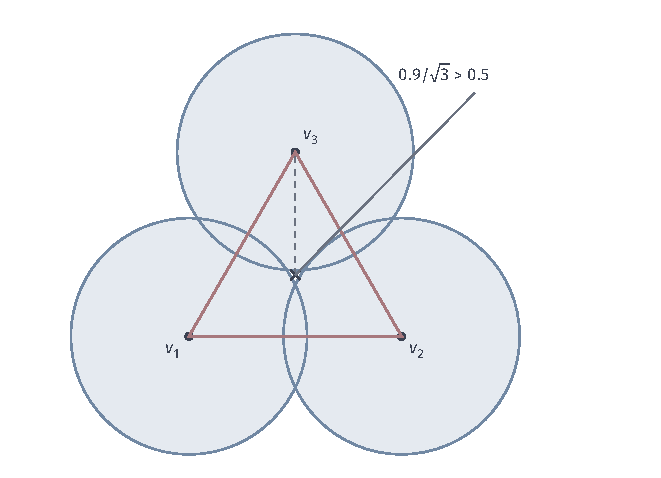
\includegraphics[width=112.0mm]{figures/01-mathematical-preliminaries-upper/02-linear-algebra-and-geometry/tikz/geometry-cech-rips-intersection/figure.pdf}
  \caption{固定同组三点比较共同交集与成对条件。正三角形边长$0.9$，
 $\varepsilon=1$，蓝色开球半径$0.5$；红色边满足两种构造的连边条件。
 三球无共同交点，Čech不含二维面，Rips含二维面。
 中心到各顶点的距离为$0.9/\sqrt3>0.5$。圆周只标开球边界，图为解析教学构造。}
 \label{fig:geometry-cech-rips-intersection}
\end{figure}

尺度变化后仍可给出明确包含关系。对任意$\eta>0$，有
\[
 \mathcal C_\varepsilon\subseteq\mathcal R_\varepsilon
 \subseteq\mathcal C_{2\varepsilon+\eta}.
\]
第一个包含关系由共同交点和三角不等式推出。
对第二个，任选一个顶点作候选共同交点，它到其余顶点的距离至多$\varepsilon$，
严格小于新球半径$\varepsilon+\eta/2$。
若全部球改用闭球，在相应定义下可取尺度常数$2$而不加$\eta$。
这些是足够的普适常数，不声称最紧；同一尺度的复形仍不能互换。

复形何时能代表球并集的拓扑，还依赖覆盖条件。良好覆盖（good cover）要求每个
非空有限交集都可连续收缩到一点；有限欧氏开球的交集为凸集，满足这项要求。
神经引理（nerve lemma）在该条件下说明Čech复形与球并集同伦等价，即二者存在相互映射，
来回复合可以连续变形到恒等映射。这里不要求两映射互为逆，所以比同胚弱：
闭区间可连续收缩到一个点，与单点空间同伦等价，却不可能与它存在双射。
这个结论不等于球并集已经恢复了未知潜在流形；
后者还需要采样覆盖和尺度条件。


复形的规模还依赖邻域尺度。开带$\mathcal M_{\mathrm{strip}}$与开矩形同胚，
中心线$\mathcal C$与开区间同胚，都没有全局环。
闭合中心线得到圆，保留横向自由度并闭合则得到二维环带；
维数不同，但都保留绕中心的一维环。只有在采样和尺度适当时，样本复形才有理由
反映这些区别。尺度太小会把采样空隙误认作分支；太大则可能跨折连边，
并以高阶面填掉原来的环。

持续同调（persistent homology）跟踪随尺度增大而嵌套的复形中，同调类何时出现、
何时消失；它提供跨尺度信息，不使所有长寿命结构自动具有真实任务语义。


硬阈值还会使略跨尺度的一对点从相连突然变为不相连。软关系改用
$\mu_{i,j}\in[0,1]$表示所选局部尺度下的邻接支持强度；
这只是隶属度，不自动是事件概率。高阶强度例如可取全部边强度的最小值，
但必须声明采用哪种规则。一种常见的合并运算是
\begin{equation}
 a\mathbin{\sqcup}b=a+b-ab=1-(1-a)(1-b),\qquad a,b\in[0,1].
 \label{eq:geometry-fuzzy-union}
\end{equation}
结果仍在$[0,1]$内；交换性由对称式给出，结合性由
$1-(1-a)(1-b)(1-c)$给出，$0$为恒等元，任一输入为$1$时输出为$1$。
这些性质使它成为明确定义的软并集，却没有提供独立事件的随机试验或联合分布。
核权重、相似度、置信度与概率的校准要求不能仅凭数值范围混同。

UMAP等方法由局部距离构造带强度的关系，再优化低维坐标以匹配这些关系；
具体目标与优化过程留给
\BookChapterRef{chap:dimensionality-reduction}{卷4《模型：经典模型》第5章“降维”}。
低维图像中的分离簇或孔洞还可能受邻居数、尺度、初始化与优化误差影响。
拓扑方法不能修复错误的局部输入：跨折捷径会被忠实组合，完全漏采的区域也无法凭空
恢复。采样覆盖、局部关系与尺度共同限制结论。

\section{扰动与稳定性}
\label{sec:geometry-stability}

缩小邻域或增加采样，改变的是逼近条件；观测稍变以后输出会变多少，则是稳定性问题。
以下分别比较映射输出、估计切空间、重构坐标与拓扑，以及路径解。
比较方向时先消去基的任意性，比较坐标时先消去距离无法识别的刚性变换，
才能把真正的响应与记录差异分开。

\subsection{运算的误差传播}
\label{sec:geometry-operation-stability}

对光滑点映射$F$，记其局部坐标表达为$\widehat F$。
在一个凸坐标区域上设$\lVert\bm J_{\widehat F}\rVert_2\leq L$，
沿区域内的线段积分得到
$\lVert\widehat F(\bm z+\bm h)-\widehat F(\bm z)\rVert_2
\leq L\lVert\bm h\rVert_2$。
跨图时还需计入两端坐标转换及度量的上下界；一个坐标中的小扰动不是坐标无关的数值。
叠加的局部放大界不超过$\sum_j|a_j|L_j$，复合不超过各步界的乘积。
若归一化分母趋零、参数化Jacobian接近降秩，这些界会变差，
因此合法运算与数值稳定是两个需要分别核对的条件。

\subsection{切空间估计的稳定性}
\label{sec:geometry-tangent-estimate-stability}

局部PCA从协方差矩阵选出一个子空间。因此，先比较理想与实际协方差，
再用上一章的子空间扰动结论把矩阵误差转成方向误差：
当$d<D$时，若理想局部协方差在第$d$与第$d+1$特征值间有间隙$\delta>0$，
而观测造成的算子范数扰动相对$\delta$足够小，则估计子空间的偏转受
$\lVert\bm E\rVert_2/\delta$控制。这里$\bm E$要包括有限样本波动、
噪声、邻域错选及非线性近似误差，不能只代入测量噪声方差。
若已知$d=D$，目标切空间就是整个环境空间$\mathbb R^D$，
无需用这条谱隙辨认方向；维数是否确为$D$仍是另一个模型判断。

缩小邻域会降低法向二阶偏差，却减少样本并压低真实信号的谱尺度；
固定噪声不会随之自动消失。邻域过大时，中心线不同位置的切线已明显转动，
PCA得到的是折中方向。对二维窄带，若样本的横向覆盖不足或宽度小于噪声尺度，
第二个方向可能难以稳定识别，但潜在对象并不因此变成一维。
固定近邻数也不能解决非均匀密度带来的变化：稀疏处覆盖范围大，稠密处范围小。
潜在对象、采样密度、嵌入弯曲、邻域尺度、谱间隙和噪声必须一起解释。


估计子空间内部的基可以旋转，输出应比较投影或主角，而不是逐列比较特征向量。
谱隙、邻域尺度和噪声一起决定能否区分切向与法向；增加样本数量不能消除固定尺度带来的几何偏差。

\subsection{坐标重构的稳定性}
\label{sec:geometry-coordinate-reconstruction-stability}

设平方距离矩阵由$\bm\Delta$变成$\bm\Delta+\bm E$。
中心化矩阵$\bm J$是正交投影，故重构Gram矩阵的扰动为
\[
 \widetilde{\bm B}-\bm B=-\tfrac12\bm J\bm E\bm J,\qquad
 \lVert\widetilde{\bm B}-\bm B\rVert_2\leq\tfrac12\lVert\bm E\rVert_2.
\]
第\ref{sec:linear-algebra-spectral-stability}节的谱扰动结论控制特征值与选定谱子空间。
选取前$d$维坐标时，需要$d$与$d+1$模态之间的谱隙；
对正特征值开平方还需要它们远离零。接近零的模态可能改变保留维数，
重复特征值则允许同一子空间内任意转动。

比较坐标前应先消去平移，再允许整体正交对齐，因为距离本来就不识别这些变换。
若点标签也改变，还须先建立点对应。小距离扰动只能在上述尺度与对齐条件下
支持坐标稳定，不能保证某个优化过程恰好返回同一朝向的坐标。

\subsection{拓扑重构的稳定性}
\label{sec:geometry-topology-reconstruction-stability}

固定阈值构造的单个复形可能发生跳变。若成对距离误差不超过$\delta$，
所有距离原本小于$\varepsilon-\delta$的边仍会被纳入，
原本大于$\varepsilon+\delta$的边仍会被排除；处在中间带内的边不能保证。
对Rips复形，这直接给出
$\mathcal R_{\varepsilon-\delta}\subseteq\widetilde{\mathcal R}_{\varepsilon}
\subseteq\mathcal R_{\varepsilon+\delta}$（左侧只在正尺度使用）。
固定尺度上的Betti数仍可能变化；跨尺度比较能把不确定性记录为尺度偏移，
但具体持续图距离的界还需要所用过滤的稳定性定理。
完全漏采的区域、错误点对应或大幅跨折连边并不属于小扰动假设，
不能从局部稳定性恢复其中的信息。

\subsection{路径解的稳定性}
\label{sec:geometry-path-solution-stability}

初值问题同时更新位置与速度。把状态记为$\bm y=(\bm z,\dot{\bm z})$以后，
它在一张坐标图中成为一阶系统$\bm y'=A(\bm y)$；
$A$由测地线方程中的速度与加速度组成。
设另一方程为$\widetilde{\bm y}'=\widetilde A(\widetilde{\bm y})$。
若两条解留在同一紧区域$K$，$A$在该区域有Lipschitz常数$L$，
且$\sup_{\bm y\in K}\lVert A(\bm y)-\widetilde A(\bm y)\rVert\leq\eta$，
积分方程给出
\[
 \lVert \bm y(t)-\widetilde{\bm y}(t)\rVert
 \leq e^{Lt}\lVert \bm y(0)-\widetilde{\bm y}(0)\rVert
       +\eta\int_0^t e^{L(t-s)}\,\mathrm ds,\qquad t\geq0.
\]
这是Gronwall不等式的直接应用，比较的是固定时间区间上的初值轨迹。
一旦路径离开该区域，常数与比较图都须重新核对。

固定端点的最短路有不同边界：距离作为最小代价可能连续，
达到它的路线却未必唯一。球面上到对跖点的最短路有多条；
终点向不同方向稍微偏离，会选出不同的大圆弧。
若局部有唯一最短路且避开使端点映射退化的位置，才可利用指数映射的局部逆
控制路线对端点的响应。初值唯一性不能替代端点最短路的稳定性条件。

\section{本章小结}
\label{sec:geometry-summary}

本章把非线性对象的局部记录、关系、运算、求解、逼近与稳定性分开建立。
坐标图记录位置，切空间规定瞬时方向，度量读出长度，路径长度的下确界定义距离；
等价关系则明确哪些输入变化被主动忽略。局部自由度、环境维数和有限观测不是同一对象。

映射微分传递速度，联络与平行移动比较不同位置的方向，指数映射和回缩产生可行的新点。
给定初值求轨迹与给定端点求最短路有不同的唯一性、存在性和稳定性边界。
点优化调用这些运算选择更新，其下降、驻点与点序列收敛仍须分别证明。

局部切平面、样本PCA、最短边路径和复形各自逼近方向、距离或拓扑。
尺度、覆盖、谱隙与噪声决定适用范围；环境弯曲、内在曲率和整体孔洞不能互相替代。
下一章把整个函数作为可变对象，沿用这里的几何域、微分与体积，
研究函数读取、函数拟合以及平滑能量所决定的函数与场优化。

\chapter{函数空间}
\label{chap:functional-analysis-and-approximation}

\newcommand{\functionalinlinetablecaption}[2]{%
  \refstepcounter{table}\label{#1}%
  \addcontentsline{lot}{table}{\protect\numberline{\thetable}#2}%
  \par\smallskip\noindent
  {\figurefont\footnotesize
   \textcolor{BookTeal}{表~\thetable}\quad #2}\par}
\newcommand{\functionalinlinefigurecaption}[2]{%
  \refstepcounter{figure}\label{#1}%
  \addcontentsline{lof}{figure}{\protect\numberline{\thefigure}#2}%
  \par\smallskip\noindent
  {\figurefont\footnotesize
   \textcolor{BookTeal}{图~\thefigure}\quad #2}\par}

把一条曲线或一个多变量函数当作整体来看待时，有限维几何里那一套“点、长度、投影、微分”仍然能提供很好的起点，却不能直接照抄。一个输入坐标并不意味着候选函数只有一个变化方向；有限几个读数也不自动确定整条函数；一个看起来漂亮的无穷展开，未必在某种整体误差下收敛。本章要处理的，正是把“函数本身”作为一个元素以后，必须重新回答的几个问题：哪些函数允许参与运算，怎样衡量两条函数之间的整体偏差，怎样合法地读取或变换一条已知函数，又怎样根据观测和目标去确定、逼近一条未知函数。

先用一个熟悉的情形说明问题出在哪里。拟合曲线时，有限维模型常把函数写成固定基函数的线性组合
\begin{equation}
  f_m(x)=\sum_{j=1}^{m}a_j\varphi_j(x).
  \label{eq:functional-finite-basis-expansion}
\end{equation}
当$m$固定时，可以把系数$(a_1,\ldots,a_m)^{\top}$当作普通向量，用欧氏距离比较两个候选解。可是一旦允许基函数数目增加，系数向量所在的维数也随之改变；同一个函数还可能在不同基下拥有完全不同的系数。此时，仅比较参数向量已经不能稳定地回答“两条函数相差多少”“有限表示能否逼近目标”以及“有限观测究竟确定了哪些函数方向”。

有限维经验在这里会遇到三类它独自回答不了的问题。其一，一条信号或曲线的记录数不是固定的：为提高精度可以不断增加基函数个数，“参数有多少个”本身会随表示规模变化，用系数向量的维数比较两条函数不再可靠。其二，许多函数只能描述成“与某条参考函数在几乎每个输入处相差多少”，这时比较的是两个无穷维对象的整体差距，而不是有限个坐标差。其三，无穷个基方向的展开是否收敛、截断多少项才够、某一点的值能否稳定读取，都没有有限维结论可以自动继承。

本章的安排正是围绕这些问题展开。第~\ref{sec:function-spaces-and-norms}节先把函数作为元素，建立范数与误差之间的关系；第~\ref{sec:weak-derivatives-sobolev}节在允许弱导数的条件下构造Sobolev空间。这两节提供后续共用的对象和结构。主体任务随后分别展开：第~\ref{sec:linear-readouts-orthogonal}节研究怎样读取函数信息并作正交表示，第~\ref{sec:linear-operators-integral-equations}节研究线性算子与积分方程，第~\ref{sec:variational-functional-fitting}节以观测和目标确定未知函数，第~\ref{sec:finite-representation-approximation}节为给定目标设计有限表示，第~\ref{sec:discrete-energy-approximation}节用有限采样表达已知函数的能量，第~\ref{sec:covering-numbers}节衡量整个函数类需要多少近似代表。这些小节按当前所求对象和操作目标分工，空间名称与算法名称并不当作互斥的类别。

需要先说明“收敛”和“稳定”这两个词在本章的含义随对象而变：正交截断是在增加保留的方向数，积分方程迭代是在增加计算次数，正则化是在改变目标参数，数据扰动则是重新求解另一个任务的解。因此相应的条件和估计都放在各自任务中讨论，不用一个不指明对象的“收敛”或“稳定”笼统代替。单个函数的逼近误差、固定记录的能量值、整个函数类的覆盖数，也分别给出各自的误差与量词。具体的场方程与几何结构则留给后续的微分方程和流形章节。

本章主要讨论实值函数与实Hilbert空间；遇到向量值函数时按分量处理。需要强调的是，对输入位置$x$求导描述的是函数自身的空间变化，而把整条未知函数当作变量作扰动，描述的则是目标如何评价候选的变化，这两类“微分”贯穿全章但始终分开。

\section{函数空间与范数}
\label{sec:function-spaces-and-norms}

把整条函数作为一个元素时，要先确定哪些函数允许参与线性运算、哪些差异算作同一个元素，再选择衡量整体偏差的规则。本节先把这项共同准备与具体范数构造分开：第~\ref{subsubsec:norm-inner-product-completeness}节建立函数元素、范数、内积与完备性等共用概念；第~\ref{subsec:constructing-function-norms}节具体构造最大偏差范数与积分范数；第~\ref{subsec:comparing-spaces-errors}节再比较不同空间、不同测度以及不同误差规则之间的关系。Banach、Hilbert与$L^p$各自表达的是不同条件，并不作为互斥类型并列。

\subsection{函数元素与空间结构}
\label{subsec:function-elements-structure}

本小节先说明空间收进什么对象，再说明要在这些对象上增加哪些结构。普通函数和几乎处处等价类的区别决定零元素如何识别；线性运算、范数、内积与完备性则分别承担组合、计量和取得极限的职责。

\subsubsection{线性空间与函数元素}
\label{subsubsec:linear-function-candidates}

同一输入集合上的函数可以逐点相加和缩放；但预先限定的候选族是否容纳这些结果，还要逐一检查。有测度时，还必须决定是否保留每个位置上的取值差异。

\paragraph{函数的线性运算与候选范围}

固定一个非空输入集合$X$，先以实值函数$f:X\to\mathbb R$为主线，并注意区分三个层次的对象：自变量$x$、$x$处的标量值$f(x)$，以及整个函数$f$。逐点定义加法和数乘
\[
  (f+g)(x)=f(x)+g(x),\qquad (cf)(x)=c\,f(x),
\]
这些运算由实数上的相应运算逐点继承，因而全体函数$X\to\mathbb R$满足线性空间的全部公理。取有限维向量值函数$f:X\to\mathbb R^r$时，按分量定义相同运算即可。

从全体函数缩小到某个候选族$V$时，不能只凭“它由若干函数组成”就称$V$为线性子空间，而要逐项检查零函数是否在其中、两个成员之和是否仍在其中、成员的标量倍是否仍在其中。连续函数族满足这些要求：两个连续函数相加或数乘后仍连续，零函数也连续；有限个生成函数$\varphi_1,\ldots,\varphi_m$的线性张成$\operatorname{span}\{\varphi_j\}$同样如此。作为对照，固定节点预算的一般非线性参数族未必封闭：两个各用$N$个节点的成员相加，可能需要多于$N$个节点才能表示，因此参数形式本身不保证线性封闭。

还要区分三个容易混淆的“维数”：输入域的维数、表示参数的数目、函数空间的维数。即使输入域只是实轴或一个非退化区间（输入维数为一），函数$1,x,x^2,\ldots$仍能提供任意多个线性无关的方向。固定深度的网络若要并行表示两个网络之和，通常必须增加宽度或节点预算，不能从“输入只有一个坐标”或“深度固定”推出候选空间有限维。把空间的成员范围固定下来以后，才进入“同一成员如何识别”的问题。

\paragraph{普通函数与几乎处处等价类}

对普通函数采用的是逐点相等：某个位置的值一旦改变，就得到不同的函数。但若误差是通过测度积分累计的，在零测集上的修改可能完全不改变误差。承接第~\ref{chap:univariate-calculus}章建立的零测集与几乎处处概念，我们需要另一种元素识别方式，记作
\[
  f\sim_\mu g\quad\Longleftrightarrow\quad f=g\text{ 在$\mu$下几乎处处成立}.
\]

在可测函数中以$[f]_\mu$表示这个等价类。加法和缩放不依赖代表的选择：若$f$换成与之几乎处处相同的$f'$，$g$换成$g'$，那么$f'+g'$与$f+g$、$cf'$与$cf$不同的位置只是两个零测集的并，仍然是零测集。这里用到的依据来自前章已由测度可数次可加性证明的结论：可数个零测集的并仍是零测集；两次换代表的例外集取有限并后仍为零测，这就保证运算结果仍几乎处处相同。于是
\[
  [f]_\mu+[g]_\mu=[f+g]_\mu,\qquad c[f]_\mu=[cf]_\mu
\]
都是良定义的。本小节只建立后面积分空间共用的对象约定；$L^p$和$L^\infty$各自的成员条件和范数要到具体构造处才定义。

零函数与“仅在一个Lebesgue零测单点取一、其余处取零”的函数是说明这一区别的最简例子：作为普通函数它们不同，作为等价类却相同。前章已从简单函数积分以及非负函数的逐段逼近证明，零测修改不影响积分；每个单点质量为零，并不使$[0,1]$上常数一的积分变成零，因为可列可加性不能被改成“不可数个单点直接求和”。这个区别目前只处理元素识别；至于某一点的值能否读取，要等到域内点值读取那一节另行判断。

图~\ref{fig:vol1-add-functional-ae-representatives}把“函数不同”与“积分空间中的元素相同”分开。绿色孤立读数不会改变Lebesgue积分，所以这两条代表在$L^p$中距离为零，但在该位置的函数值仍不同。
\begin{figure}[!htb]
  \centering
  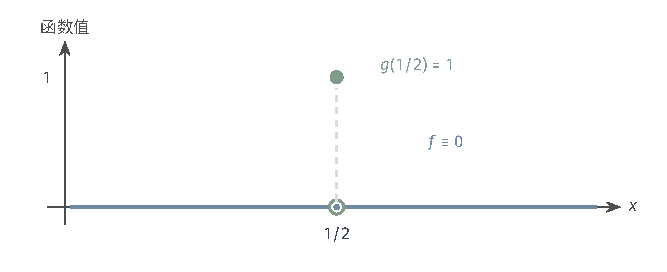
\includegraphics[width=112mm]{figures/01-mathematical-preliminaries-upper/02-linear-algebra-and-geometry/tikz/comprehension-additions/functional-ae-representatives.pdf}
  \caption{同一积分元素的不同代表。定义域为$[0,1]$并用Lebesgue测度，$f\equiv0$，$g$除$g(1/2)=1$外也为零。绿空心圈表示$g$不在该点取零，圈内蓝点保留$f(1/2)=0$。单点集合测度为零，故任意$1\le p<\infty$下$\|f-g\|_{L^p}=0$；点值读取却不同。}
  \label{fig:vol1-add-functional-ae-representatives}
\end{figure}

\subsubsection{范数、内积与完备性}
\label{subsubsec:norm-inner-product-completeness}

候选及元素相等的含义确定以后，误差公式还必须满足相应公理，极限过程也必须能在同一空间内完成。本节先把范数、Banach条件和Hilbert条件各自要回答的对象与条件说清，后面的具体空间再据此逐一核验。

\paragraph{范数与函数距离}

要比较$f$与$g$的整体偏差，自然的做法是先为单个函数确定“大小”，再由差$f-g$得到两函数之间的距离。在已经确定元素识别的实线性空间$V$上，范数是一个映射$\|\cdot\|:V\to[0,\infty)$，满足三条要求
\begin{align*}
  &\|f\|=0\ \Longleftrightarrow\ f=0,\\
  &\|cf\|=|c|\,\|f\|,\\
  &\|f+g\|\le\|f\|+\|g\|.
\end{align*}
这三条分别保证零误差能被准确识别、按常数缩放时误差一致，以及两段误差合起来不超过各自之和，最后一条就是\term{三角不等式}。令
\[
  d(f,g)=\|f-g\|,
\]
便能把范数公理逐项转成度量公理，从而可以直接回用第~\ref{chap:function-limits}章关于度量空间中柯西列与完备性的结论。需要强调，如果某个公式在普通函数上只能让非零函数长度为零，就必须先处理这些零方向或改用等价类，不能直接宣布它在原候选上是范数。

同一对函数可以用不同范数衡量：有的强调最大偏差，有的强调积分累计，选哪一种取决于当前真正要控制的误差。这里先建立公理与用途；具体公式是否有限、是否满足三角不等式、能识别何种零元素，分别在下一小节核验。

\paragraph{范数空间的完备性与Banach空间}

对范数空间中的一个柯西列，要区分两件事：“各项彼此越来越接近”与“在候选空间内确实存在一个极限”。若每个范数柯西列都存在$V$中的范数极限，就称$V$为\term{Banach空间}。完备性这个条件同时包含所选候选和所选范数，不能只给出一个误差公式就把完备性视为当然。

后面证明具体空间完备时，都会遵循同一条路线：先构造一个候选极限，再证明它保留了该空间的成员条件，最后证明范数误差趋于零。在无限维情形，子空间是否闭、有界列能否抽出范数收敛子列、线性映射是否连续，都必须分别验证，这些性质并不因线性运算成立就自动继承。这里先列清判断边界，后面的投影、读取和算子问题再使用各自的条件。

\paragraph{内积及Hilbert空间}

当任务还要比较函数方向、正交分量或平方误差时，需要在实线性空间上引入内积$\langle f,g\rangle$，要求它对两个变量都是双线性的、对称的，并且$\langle f,f\rangle\ge0$、仅在$f=0$时为零。由
\[
  \|f\|=\sqrt{\langle f,f\rangle}
\]
得到长度。这条长度确实满足三角不等式：对任意实数$t$，
\[
  0\le\|f-tg\|^2=\|f\|^2-2t\langle f,g\rangle+t^2\|g\|^2
\]
是关于$t$的非负二次式，故其判别式不大于零，
\[
  |\langle f,g\rangle|\le\|f\|\|g\|,
\]
即Cauchy--Schwarz不等式；再由
\[
  \|f+g\|^2=\|f\|^2+2\langle f,g\rangle+\|g\|^2
  \le(\|f\|+\|g\|)^2
\]
得到三角不等式。

在这个诱导范数下完备的内积空间称为\term{Hilbert空间}，因此Hilbert空间同时也是Banach空间。一般范数未必来自内积，“是否存在内积”与“是否完备”是两个不同的判断。后面的$L^2$、$W^{k,2}$以及正交读取都会注明使用的是哪个内积、完备性从哪里取得。还要提醒一句，内积给出的是函数空间中的正交关系，并不是两条函数图像在平面中相交的几何角度；图~\ref{fig:vol1-add-functional-integral-orthogonality}正好说明这一点。

\begin{figure}[!htb]
  \centering
  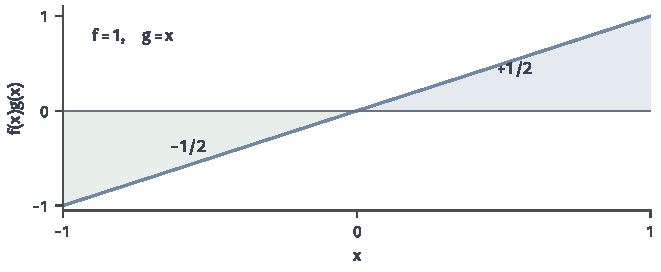
\includegraphics[width=112mm]{figures/01-mathematical-preliminaries-upper/02-linear-algebra-and-geometry/matplotlib/comprehension-additions/functional-integral-orthogonality.pdf}
  \caption{整函数的正交由内积决定。在$[-1,1]$上用Lebesgue积分内积，取$f(x)=1$、$g(x)=x$。图中曲线是乘积$f(x)g(x)=x$，右侧蓝色区域积分为$1/2$，左侧绿色区域积分为$-1/2$，相加为零。因此两函数正交，所画曲线的平面倾角不承担函数空间夹角的含义。}
  \label{fig:vol1-add-functional-integral-orthogonality}
\end{figure}

\subsection{函数范数的构造}
\label{subsec:constructing-function-norms}

固定一对函数后，按偏差的汇总规则可以分为最大偏差控制和积分累计两类。前者再区分处处控制与允许零测例外的控制，后者固定有限的$p$次累计。每种构造都要说清成员、零元素和极限归属，不把具体空间名称当成互斥类别。

\subsubsection{上确界范数}
\label{subsubsec:supremum-norm}

比较两条曲线时，最大偏差控制要求对允许的全部位置给出一个共同上界。普通函数逐点识别与几乎处处等价类的识别不同，因此一致范数和本质上确界范数要分别构造，不能用一个代表的普通上确界代替等价类的本质上界。

\paragraph{连续函数的一致范数}

固定紧区间$[a,b]$上的实连续函数空间$C([a,b])$。为了同时控制所有位置的偏差，定义
\[
  \|f\|_\infty=\sup_{x\in[a,b]}|f(x)|,\qquad d_\infty(f,g)=\|f-g\|_\infty.
\]
连续性与紧性保证这个上确界有限。范数公理逐条成立：$\|f\|_\infty=0$意味着连续函数$f$在每一点为零，即$f=0$；齐次性由逐点缩放后取上确界直接得到；三角不等式由$|f(x)+g(x)|\le|f(x)|+|g(x)|\le\|f\|_\infty+\|g\|_\infty$对每个$x$成立、再取上确界得到，整个函数便成为范数空间中的一个元素。

取一致范数下的一个柯西列$(f_n)$。固定$x$后，
\[
  |f_n(x)-f_m(x)|\le\|f_n-f_m\|_\infty,
\]
所以右边的标量序列是柯西列，由实数完备性逐点定义$f(x)=\lim_n f_n(x)$。这一步只是构造出候选极限，还没有证明一致收敛或连续性。

一致收敛由共同误差界取得：给定$\varepsilon>0$，取$N$使$n,m\ge N$时$\|f_n-f_m\|_\infty<\varepsilon$；对固定的$x$与$n\ge N$，令$m\to\infty$，由绝对值连续得
\[
  |f_n(x)-f(x)|\le\varepsilon,
\]
该界不依赖$x$，故$\sup_x|f_n(x)-f(x)|\to0$。这一步把逐点构造提升为统一误差控制，是证明极限留在空间内的中间环节。

再固定位置$x_0$，把$|f(x)-f(x_0)|$拆成两端的$f-f_N$误差与中间的$f_N(x)-f_N(x_0)$：先选$N$使两端统一地小于$\varepsilon/3$，再利用$f_N$的连续性选择邻域使中间一项也小于$\varepsilon/3$，三项相加得$|f(x)-f(x_0)|<\varepsilon$，便得到$f$连续。因此极限仍留在$C([a,b])$，与上一步合起来才完成Banach性质的证明。

若输入域不紧，连续函数可能无界，普通上确界便可能为无穷；这时要改选有界连续函数空间或另加增长条件。下一项保持最大偏差的汇总规则，只改变零测例外的约定，而不把输入域不紧的问题误当成本质上界的定义理由。

\paragraph{本质上确界范数}

在测度空间$(X,\mathcal A,\mu)$上，积分任务允许忽略零测集，因此从可测实函数的几乎处处等价类出发，定义
\[
  \|[f]_\mu\|_{L^\infty(\mu)}
  =\inf\{M\ge0:|f|\le M\text{ 在$\mu$下几乎处处成立}\},
\]
以该值有限者构成$L^\infty(\mu)$。\term{本质上确界}不随代表变化：若$g$与$f$几乎处处相等，每个使$|f|\le M$成立的零测例外集与$\{f\neq g\}$取并后仍为零测集，同一$M$也控制$g$；但同一等价类各代表的普通上确界可能差别很大。

范数公理逐项核对。正定性：若$\|f\|_\infty=0$，则对每个正整数$k$都有$|f|\le1/k$几乎处处；这些可测例外集的可数并为零测集，其外$|f|\le1/k$对所有$k$同时成立，故$f=0$几乎处处。齐次性由$|cf|=|c||f|$逐点成立直接得到。三角不等式：若$|f|\le C$在零集$N_f$外成立、$|g|\le D$在零集$N_g$外成立，则在$X\setminus(N_f\cup N_g)$上$|f+g|\le C+D$，例外集仍为零测集，故$\|f+g\|_\infty\le C+D$；对$C,D$各自取下确界，得到$\|f+g\|_\infty\le\|f\|_\infty+\|g\|_\infty$。

完备性证明要小心处理例外集。取$L^\infty$柯西列并选可测代表$f_n$。每项几乎处处有界给出可测零集$N_n^0$，使$|f_n|\le M_n$于$X\setminus N_n^0$；柯西性给出：对每个$n,m$与每个正整数$r$，
\[
  |f_n-f_m|\le\|f_n-f_m\|_\infty+\tfrac1r
\]
几乎处处成立，例外集记为$N_{nmr}$。前章已证明可数个零测集的并仍是零测集，故
\[
  N=\left(\bigcup_n N_n^0\right)\cup\left(\bigcup_{n,m,r\in\mathbb N}N_{nmr}\right)
\]
是单一可测零集。在$X\setminus N$上所有不等式对所有下标同时成立，令$r\to\infty$后，所有需要的差值界便同时成立。不能为每个位置各选一个例外集。

在这个共同补集上，范数柯西性给出了真正的一致柯西性。先固定一项$f_1$的有界控制；柯西列$\{\|f_n-f_1\|_\infty\}$有界，设其上界为$C$，则
\[
  |f_n(x)|\le|f_1(x)|+|f_n(x)-f_1(x)|\le M_1+C,\qquad x\in X\setminus N,
\]
故逐点极限$f(x)=\lim_n f_n(x)$在$X\setminus N$上存在且一致有界；在$N$上补零，并由逐点极限与可测零集改值的可测性，$f$是可测代表且$f\in L^\infty$。把共同柯西界的一端送到极限：对$x\in X\setminus N$，
\[
  |f_n(x)-f(x)|=\lim_{m\to\infty}|f_n(x)-f_m(x)|
  \le\limsup_{m\to\infty}\|f_n-f_m\|_\infty,
\]
这在零集$N$之外成立，故$\|f_n-f\|_\infty\le\limsup_m\|f_n-f_m\|_\infty\to0$。于是得到本质上确界范数收敛以及极限的有限本质上界，从而证明$L^\infty$完备。零测修改不改变元素，仍不回答某一指定点值是否确定——这项读取问题要交给后面的点值良定义性处理。

\subsubsection{积分范数}
\label{subsubsec:integral-norms}

若总体偏差按测度累计，就要先选定$p$次累计以及有限积分的成员，再证明范数性质和完备性。下列三个有标题的单元分别负责对象构造、误差公理和空间内极限，不把证明中的每个临时步骤另升成标题。

\paragraph{$L^p$空间及其范数}

固定测度空间与$1\le p<\infty$，从满足
\[
  \int_X|f|^p\,\mathrm d\mu<\infty
\]
的可测实函数出发，按几乎处处相等取等价类。以这些等价类组成$L^p(\mu)$；零积分差识别的是同一等价类，而不是每个位置的值都相同。为了使整体缩放$f\mapsto cf$对应误差乘$|c|$，定义
\[
  \|[f]\|_p=\left(\int_X|f|^p\,\mathrm d\mu\right)^{1/p},
\]
并核对换代表不改变数值：前章已证明零测集上的改动不改变勒贝格积分。$p=1$累计绝对偏差，$p=2$累计平方偏差后开方，一般的$p$改变对大偏差的计价，公式的用途先于不等式证明说明。下文常用代表元$f$代写等价类$[f]$，并简记范数为$\|f\|_p$。

在$[0,1]$的Lebesgue测度下取$f_n(x)=x^n$，可算得
\[
  \|f_n\|_p=\left(\int_0^1x^{np}\,\mathrm dx\right)^{1/p}
  =\left(\frac{1}{np+1}\right)^{1/p}.
\]
它的逐点极限在$x<1$时为零、在$x=1$时为一，仍代表零积分元素；而普通一致范数恒为一。这个例子同时区分了普通函数极限、积分等价类和最大偏差，后面比较各种收敛时只回用这里的计算结果。

现有公式还没有自动保证三角不等式与空间完备性。先用
\[
  |f+g|^p\le 2^{p-1}(|f|^p+|g|^p)
\]
说明成员对加法封闭：逐点有
\[
  (a+b)^p\le(2\max\{a,b\})^p=2^p\max\{a^p,b^p\}\le2^{p-1}(a^p+b^p),
\]
积分后即知$f,g\in L^p$时$f+g\in L^p$。有限$p$与前面的$L^\infty$构造始终保持各自条件。

\paragraph{Hölder不等式与范数性质}

对$1<p<\infty$固定共轭指数$q=p/(p-1)$，则$1/p+1/q=1$。先证明标量Young不等式：对$a,b\ge0$，
\[
  ab\le\frac{a^p}{p}+\frac{b^q}{q}.
\]
固定$b\ge0$，考虑关于$s\ge0$的函数$F(s)=s^p/p-bs$。其导数$s^{p-1}-b$在$s_*=b^{1/(p-1)}=b^{q/p}$处为零，且$F''(s)=(p-1)s^{p-2}>0$，故该处取最小值；代入得$F(s_*)=-b^q/q$，于是$F(s)\ge-b^q/q$对所有$s\ge0$成立，取$s=a$即得Young不等式。

对非零且有限范数的函数，在Young不等式中取
\[
  a=\frac{|f|}{\|f\|_p},\qquad b=\frac{|g|}{\|g\|_q},
\]
积分并复用前章积分的线性与单调性，得到
\[
  \frac{1}{\|f\|_p\|g\|_q}\int_X|fg|\,\mathrm d\mu
  \le\frac{1}{p\|f\|_p^p}\int_X|f|^p\,\mathrm d\mu
  +\frac{1}{q\|g\|_q^q}\int_X|g|^q\,\mathrm d\mu
  =\frac1p+\frac1q=1,
\]
再恢复尺度，得到Hölder不等式
\[
  \int_X|fg|\,\mathrm d\mu\le\|f\|_p\|g\|_q.
\]
若$\|f\|_p=0$，由前章零积分判别定理（$\int|f|=0$当且仅当$f=0$几乎处处）知$fg=0$几乎处处，不等式为平凡$0\le0$；端点$L^1$与$L^\infty$的配对直接由$|fg|\le|f|\|g\|_\infty$积分估计。

已知$f+g\in L^p$后，\term{Minkowski不等式}按如下推导。先由$|f+g|^p=|f+g|^{p-1}|f+g|\le|f+g|^{p-1}(|f|+|g|)$，把$\int|f+g|^p$写成
\[
  \int_X|f+g|^{p-1}|f|\,\mathrm d\mu
  +\int_X|f+g|^{p-1}|g|\,\mathrm d\mu.
\]
两项分别对$|f+g|^{p-1}$与$|f|$、$|g|$应用Hölder。由$(p-1)q=p$，
\[
\begin{aligned}
  \int_X|f+g|^{p-1}|f|\,\mathrm d\mu
  &\le\left(\int_X|f+g|^{(p-1)q}\,\mathrm d\mu\right)^{1/q}\|f\|_p\\
  &=\left(\int_X|f+g|^p\,\mathrm d\mu\right)^{1/q}\|f\|_p,
\end{aligned}
\]
第二项同理，合并得
\[
  \int_X|f+g|^p\,\mathrm d\mu
  \le\left(\int_X|f+g|^p\,\mathrm d\mu\right)^{1/q}
  \bigl(\|f\|_p+\|g\|_p\bigr).
\]
若$\|f+g\|_p>0$，两端同除$(\int|f+g|^p)^{1/q}$，利用$p-p/q=p(1-1/q)=p/p=1$，便得到\term{Minkowski不等式}
\[
  \|f+g\|_p\le\|f\|_p+\|g\|_p.
\]
若$\|f+g\|_p=0$，$f+g$为零等价类，不等式平凡成立。零值情形必须单独落下，不能略过约去项所需的条件。$p=1$时直接对绝对值的逐点三角不等式积分，与前两段合起来完成所有有限$1\le p<\infty$的范数性质。两点计数测度下取两个不相交的单位向量可以看出范围$p\ge1$的实际作用：当$0<p<1$时，两者之和的$p$次累计根为$2^{1/p}>2$，同一公式在该范围不满足范数\term{三角不等式}。

对$p=2$给出
\[
  \langle f,g\rangle=\int_Xfg\,\mathrm d\mu,
\]
由Hölder保证积分存在，逐项核对它是实内积并识别其诱导范数。此时只得到内积结构；等下一单元的完备性完成后，才能据此称$L^2$为Hilbert空间。

\paragraph{$L^p$空间的完备性}

对$L^p$柯西列$(f_n)$，依次选取子列$(f_{n_k})$使
\[
  \sum_k\|f_{n_{k+1}}-f_{n_k}\|_p<\infty.
\]
之所以能选出这样“快速缩小相邻差”的子列，是柯西条件的直接推论：递归取$n_k$，使$n,m\ge n_k$时$\|f_n-f_m\|_p<2^{-k}$。选好子列后再取可测代表，不能把整个原列的逐点收敛当成前提。

对有限部分和
\[
  S_m=|f_{n_1}|+\sum_{k=1}^{m}|f_{n_{k+1}}-f_{n_k}|
\]
使用Minkowski不等式，得到与$m$无关的有限范数上界：
\[
  \|S_m\|_p\le\|f_{n_1}\|_p+\sum_{k=1}^m\|f_{n_{k+1}}-f_{n_k}\|_p\le C.
\]
数列$S_m$逐点单调不减，故$S_m^p\uparrow S^p$。由前章的单调收敛定理，
\[
  \int_XS^p\,\mathrm d\mu=\lim_{m\to\infty}\int_XS_m^p\,\mathrm d\mu\le C^p<\infty,
\]
取得$S=\lim_mS_m\in L^p$，故$S<\infty$几乎处处。这一步补出了“无穷差分累计仍可被积分控制”的依据。

在$S$有限处，差分级数$\sum_k(f_{n_{k+1}}-f_{n_k})$被$S$控制而绝对收敛，定义
\[
  f=f_{n_1}+\sum_k(f_{n_{k+1}}-f_{n_k}),
\]
并在可测零例外集$\{S=\infty\}$上置零。由逐点极限的可测性以及$|f|\le S$，得到可测代表及有限的$p$次积分，确认候选极限属于原来的$L^p$空间。

再用同样的有限和估计控制尾和：对部分和$T_{j,m}=\sum_{k=j}^m(f_{n_{k+1}}-f_{n_k})$，Minkowski给$\|T_{j,m}\|_p\le\sum_{k=j}^m\|f_{n_{k+1}}-f_{n_k}\|_p$；$m\to\infty$时$T_{j,m}\to f-f_{n_j}$几乎处处，由前章Fatou引理，
\[
\begin{aligned}
  \|f-f_{n_j}\|_p^p
  &=\int\liminf_m|T_{j,m}|^p\,\mathrm d\mu\\
  &\le\liminf_m\int|T_{j,m}|^p\,\mathrm d\mu\\
  &\le\left(\sum_{k\ge j}\|f_{n_{k+1}}-f_{n_k}\|_p\right)^p,
\end{aligned}
\]
得到
\[
  \|f-f_{n_j}\|_p\le\sum_{k\ge j}\|f_{n_{k+1}}-f_{n_k}\|_p\to0.
\]
最后把$\|f_n-f\|_p$拆成“原列到某个固定子列项的柯西误差”与“该子列项到$f$的误差”：先取$j$足够小使第二项小，再用柯西性取$n,n_j$足够接近使第一项小，便取得整列收敛；只构造出子列极限尚不足以得到这一结论。汇合成员资格、范数收敛和前面的内积结构可知：所有$1\le p<\infty$的$L^p$都是Banach空间，$L^2$进一步是Hilbert空间。与本质上确界范数的单独证明相对照，这里明确没有把$p=\infty$混入有限$p$的累计公式。

\subsection{函数空间与误差的比较}
\label{subsec:comparing-spaces-errors}

具体空间建立以后，本节分别问三件事：成员能否转入另一空间，更换测度后是否仍识别相同元素，以及不同误差趋零能推出哪些结论。三个问题各有对象和条件，先处理成员与零集，再用定量不等式比较误差；包含关系本身不替代范数比较。

\subsubsection{函数空间的包含关系}
\label{subsubsec:inclusion-relations}

同一个普通函数满足较强条件时，可能合法地成为另一空间的元素；但进入等价类空间时，要说清这里的“包含”究竟是集合包含还是自然映射。

固定输入域与连续生成函数$\varphi_1,\ldots,\varphi_m$，由连续性对有限线性组合封闭，得到
\[
  \operatorname{span}\{\varphi_j\}\subset C(X).
\]
这是真正的普通函数集合包含，不需要先取几乎处处等价类。

对同一测度且$0<\mu(X)<\infty$、$1\le p<q<\infty$，把已证明的Hölder用于$|f|^p\cdot1$，使用共轭指数$q/p$与$q/(q-p)$，得到
\[
  \int_X|f|^p\,\mathrm d\mu
  \le\left(\int_X|f|^{q}\,\mathrm d\mu\right)^{p/q}
  \left(\int_X1^{q/(q-p)}\,\mathrm d\mu\right)^{(q-p)/q}
  =\|f\|_q^p\,\mu(X)^{(q-p)/q},
\]
两端开$p$次方，即
\begin{equation}
  \|f\|_p\le\mu(X)^{1/p-1/q}\|f\|_q.
  \label{eq:functional-lp-inclusion}
\end{equation}
右端有限才推出$L^q\subseteq L^p$；$q=\infty$时由本质上界积分另得相同形式的端点估计：$\int_X|f|^p\,\mathrm d\mu\le\|f\|_\infty^p\mu(X)$，开$p$次方得$\|f\|_p\le\mu(X)^{1/p}\|f\|_\infty$，不重复Hölder证明。

紧域上的连续函数有界，有限Borel测度由此保证其有限$p$次积分的成员资格。把普通函数送入积分空间时要明确写成$f\mapsto[f]_\mu$；若测度不是全支撑，不同的连续函数仍可能代表同一元素，因此这是自然映射，只有在核实单射条件后才能把它当作函数空间嵌入。

无限总测度下，式~\eqref{eq:functional-lp-inclusion}中的质量常数不再给出有限控制。例如无限Lebesgue测度上的常数一属于$L^\infty$，却不属于任何有限$p$的$L^p$。这就界定了包含结论的范围。同一测度下成员关系清楚以后，下一题保持函数不变，转向改变计价测度会发生什么。

\subsubsection{换测度后的元素与范数}
\label{subsubsec:change-of-measure}

在同一可测集合上改用另一测度，首先可能改变的是“哪些差异完全不计价”，随后才是误差大小的改变。测度间的零集关系在此本地固定：对两个测度$\mu,\nu$，若每个$\mu$零测集也是$\nu$零测集，称$\nu$关于$\mu$\term{绝对连续}，记作$\nu\ll\mu$；若$\mu\ll\nu$与$\nu\ll\mu$同时成立，两测度有完全相同的零集，称为相互绝对连续（等价测度）。下面把这些关系落实到函数元素和范数上。

\paragraph{零集关系与等价类识别}

固定共同可测空间上的$\mu,\nu$，回用$f\sim_\mu g$当且仅当$f=g$在$\mu$下几乎处处。若$\nu\ll\mu$，则$\mu$零测的差异也是$\nu$零测的，因而映射$[f]_\mu\mapsto[f]_\nu$在可测函数的等价类层面不依赖代表。这个结论并没有自动保证一个$L^p(\mu)$成员还具有有限的$\nu$积分。

如果两测度相互绝对连续，它们识别相同的零差异；若只在一个方向绝对连续，新测度可能把更多函数归为同一元素。以$[0,1]$上$\mathrm d\nu=w\,\mathrm d\mu$为例：这里$\nu(B)=\int_Bw\,\mathrm d\mu$是一个测度，其可数可加性由前章非负函数项级数的逐项积分定理保证，且它自动满足$\nu\ll\mu$。令$w$在一块原本正测度的区域上为零，那么两个只在该区域不同的函数，可由不同的$\mu$类合成同一个$\nu$类。这里要把相互绝对连续（等价测度）与“相等测度”区分开：$\mu$与$2\mu$有相同的零集，却是不同的测度。另外，“任意$\nu\ll\mu$都有形如$\mathrm d\nu=w\,\mathrm d\mu$的密度”这一反方向结论是Radon--Nikodym定理，其一般证明见教材\scite{math-folland1999real}，本节只使用直接给出的加权测度，不把该定理当作本地已证结论。

即使$w>0$几乎处处、零集识别相同，若$w$没有统一上界或正下界，也不能据此给出两个范数之间统一的比较常数。这里先把元素识别与定量大小分开，正说明下一单元增加密度界的必要性；指定点值的读取仍留到点值读取一节处理。

\paragraph{密度界与范数换算}

在$\mathrm d\nu=w\,\mathrm d\mu$及有限$1\le p<\infty$下，把差函数$h=f-g$代入相对密度的积分公式，先写
\[
  \|h\|_{L^p(\nu)}^p=\int_X|h|^pw\,\mathrm d\mu.
\]
若$w\le C<\infty$几乎处处，便由积分单调性逐步得到
\[
  \|h\|_{L^p(\nu)}^p\le C\int_X|h|^p\,\mathrm d\mu=C\|h\|_{L^p(\mu)}^p,
\qquad
  \|h\|_{L^p(\nu)}\le C^{1/p}\|h\|_{L^p(\mu)}.
\]
同一估计同时保证了从$L^p(\mu)$到$L^p(\nu)$的成员转换，这一点不能从绝对连续单独推出。

若再有$0<c\le w$几乎处处，反向得到
\[
  c^{1/p}\|h\|_{L^p(\mu)}\le\|h\|_{L^p(\nu)},
\]
从而两边成员资格一致，误差由双向常数控制。$L^\infty$另外依赖零集识别：等价测度给出相同的本质上确界，不能给它硬套有限$p$的$C^{1/p}$推导；只有单向绝对连续时，只能得到相应方向的本质上界控制。回头看例子可知，比较时必须同时注明测度、指数以及密度上下界。前两段处理的是同一差函数在两种计价规则中的大小，尚未涉及一列函数如何趋近；下一题就在这些量化控制上建立收敛蕴含。

\subsubsection{函数距离与收敛方式的比较}
\label{subsubsec:convergence-comparison}

固定候选、元素识别和误差以后，“误差趋零”才有具体含义。本单元共同定义范数收敛、逐点收敛和一致收敛，并用不同范数与同一序列检验蕴含关系；后面的计算迭代、截断和正则化解族只复用这些判断，不重新定义。

\paragraph{范数、逐点与一致收敛}

固定范数空间中的候选极限$f$，定义$f_n\to f$为$\|f_n-f\|\to0$，并写清这个范数及其测度。若空间元素是几乎处处等价类，所比较的是类的误差，不能不选代表就把它解释成每点函数值都收敛。

对同一输入集合上的普通函数，逐点收敛要求对每个固定的$x$都有$f_n(x)\to f(x)$，但允许所需序号随$x$而变。一致收敛则要求：对每个$\varepsilon>0$，存在一个统一的$N$，使所有$n\ge N$和所有$x$都满足
\[
  |f_n(x)-f(x)|<\varepsilon.
\]
共同阈值解释了为什么一致控制强于逐点控制。

用前面$x^n$的计算结果比较：它在$[0,1]$上逐点趋于一条“端点为一、其余为零”的函数，有限$p$范数趋零，却没有一致地趋于该逐点极限。三个陈述分别使用普通函数极限、积分零元素和统一偏差，并不相互矛盾。

\paragraph{范数比较与收敛蕴含}

对同一对函数的差$h=f-g$，若已经取得
\[
  \|h\|_A\le C\|h\|_B
\]
且$C$不随函数序号改变，那么$B$范数误差趋零才能传成$A$范数误差趋零。双向常数控制给出两种范数收敛等价；“同一函数集合”或各自范数有限都不能替代这项统一估计。

回用有限测度包含中的估计，得到$L^q$收敛推出$L^p$收敛；回用
\[
  \|h\|_p\le\mu(X)^{1/p}\|h\|_\infty,
\]
得到有限总测度下一致误差趋零推出$L^p$误差趋零。这里是从已建立的常数转为序列结论，不再重做Hölder证明。

改成实轴上的无限Lebesgue测度，取
\[
  h_n=\tfrac1n\,\mathbb I_{[0,n^2]}.
\]
直接算得普通上确界为$1/n\to0$，而
\[
  \|h_n\|_2^2=\frac{1}{n^2}\cdot n^2=1;
\]
支撑范围同时扩大使有限测度结论失效，不能只看函数高度判断积分误差。更换测度后的收敛蕴含同样使用上一题的密度界，并保留其方向和常数。无论更换$p$、测度还是最大偏差规则，都要先给定同一差函数的定量控制，再谈误差极限；由范数到具体读数还要检验相应读取的有界性，这项新增问题由点值读取的有界性展开，不在此复述连续尖峰证明。

\paragraph{逐点判断与积分误差的边界}

为检验$L^p$收敛能否自动控制整列的每点行为，在$[0,1)$上按层排列二进区间指示函数：第$k$层依次取
\[
  [j2^{-k},(j+1)2^{-k}),\qquad j=0,\ldots,2^k-1,
\]
再按层展开成一个序列。每项的$L^p$范数为
\[
  \|h_{k,j}\|_p=\left(\int_{j2^{-k}}^{(j+1)2^{-k}}1\,\mathrm dx\right)^{1/p}=2^{-k/p},
\]
随序号增长而趋零。但对每个固定的$x\in[0,1)$，每一层恰有一项在该点取一，而充分大的层里也有其他项取零。因此整列在该点反复出现零和一，不逐点收敛；这是真正的同一列代表函数行为，不是任意更改零测点造成的现象，也不排除另选子列的结论。

反方向固定$[0,1]$上的Lebesgue测度，取$g_n=n\,\mathbb I_{(0,1/n)}$。每个位置最终都落在支撑外，所以$g_n$处处趋零，而
\[
  \|g_n\|_2^2=n;
\]
逐点阈值随位置变化并允许窄区间上的峰值增长，不能单独控制积分误差。若要由逐点或几乎处处极限转移积分，必须另给支配等条件并回用前章的支配收敛定理。

\paragraph{系数距离与函数距离}

对$[-1,1]$及$\mathrm d\mu=\mathrm dt/2$，固定仿射表示$f(t)=a+bt$。把两个函数之差$\delta a+\delta bt$平方积分，交叉项因对称区间上$t$的积分为零，得到
\[
  \|\delta a+\delta bt\|_{L^2}^2=(\delta a)^2+\frac{(\delta b)^2}{3},
\]
而原系数的欧氏距离平方为$(\delta a)^2+(\delta b)^2$。这个差异来源于基函数在当前内积下的尺度，可概括为有限表示的函数误差二次型
\[
  \delta c^{\top}G\,\delta c,\qquad G_{ij}=\langle\varphi_i,\varphi_j\rangle.
\]
改变基必须连同系数和\term{Gram矩阵}一起变换；这里比较的是既定表示下的两种误差，记录转换与冗余方向的完整讨论由后面的系数与读数转换承接。

\section{弱导数与Sobolev空间}
\label{sec:weak-derivatives-sobolev}

绝对值函数在尖点没有经典导数，但把导数转移给光滑测试函数以后，积分恒等式仍然能够表达它的变化。本节先建立测试函数与分布的共同配对，再判断分布导数何时能由普通函数表示，最后把函数及规定阶弱导的积分控制组织成Sobolev空间。点值和边界迹属于随后读取任务的内容。

\subsection{测试函数与分布}
\label{subsec:test-functions-distributions}

把导数转移到测试函数之前，必须说明测试函数是什么、为什么能避开边界，以及什么对象可以与它配对。两个子题分别建立接收测试的空间和作用于测试的连续线性泛函，给出弱导定义的共同对象。

\subsubsection{紧支撑测试与局部可积函数}
\label{subsubsec:test-functions-local-integrable}

固定非空开域$\Omega\subset\mathbb R^d$，取光滑且支撑紧含于$\Omega$的函数$\varphi\in C_c^\infty(\Omega)$。可以先在内部一块区域上想象一个光滑凸起：函数在靠近域边界之前就已经恒为零，因此分部积分时不会留下边界项。把这样的光滑凸起归一化到积分为一，还能为后面的局部平滑做准备。

定义$f\in L^1_{\mathrm{loc}}(\Omega)$表示：在每个紧子集$K\Subset\Omega$上，$|f|$的积分都有限。测试函数有界且只占一块紧支撑，因此
\[
  \int_\Omega f\varphi\,\mathrm dx
\]
有限。这说明不需要先要求$f$在整个域上可积，也能合法地形成局部测试配对。

为了把“连续作用”与任意代数线性作用区分开，还要说明测试函数序列趋零的条件：它们的全部支撑落在同一个紧集内，并且每个阶数的导数都一致趋零。支撑共同受限和各阶控制这两条都不能省；下一题正是用这种收敛说明分布的连续性，而不把测试空间误当成只带一个上确界范数的空间。

\subsubsection{分布及普通函数的表示}
\label{subsubsec:distributions-regular}

\paragraph{分布的定义}

“给每个测试函数一个线性读数”自然引出分布：分布$T$就是测试函数空间上的连续线性泛函。连续性可以写成本地可核对的估计：对每个紧集$K\Subset\Omega$，存在常数$C_K$和有限整数$m_K$，使支撑在$K$内的测试满足
\[
  |T(\varphi)|\le C_K\max_{|\alpha|\le m_K}\sup|D^\alpha\varphi|.
\]
这里的多重指标$\alpha=(\alpha_1,\ldots,\alpha_d)$是一组非负整数，$|\alpha|=\alpha_1+\cdots+\alpha_d$是总阶数，$D^\alpha\varphi=\partial_1^{\alpha_1}\cdots\partial_d^{\alpha_d}\varphi$是对应偏导。

这个估计说明：上一题那种“共同紧支撑、各阶导数一致趋零”的测试序列趋零时，读数$T(\varphi)$也趋零。因此分布保留了对光滑测试变化的连续响应，而任意代数线性映射并不自动满足这一点。本节只使用这一本地连续性，不展开完整的局部凸拓扑理论。

\paragraph{局部可积函数与Dirac分布}

对$f\in L^1_{\mathrm{loc}}$定义
\[
  T_f(\varphi)=\int_\Omega f\varphi\,\mathrm dx,
\]
由
\[
  |T_f(\varphi)|\le\left(\int_K|f|\,\mathrm dx\right)\sup_K|\varphi|
\]
即可核对线性和连续性。称这类分布由普通函数表示；换成几乎处处相同的$f$不改变分布。要注意，它输出读数的对象是光滑测试，而不是任意函数在某一点的值。

另取$x_0\in\Omega$，以
\[
  \delta_{x_0}(\varphi)=\varphi(x_0)
\]
定义Dirac分布。上确界控制即可证明其连续性，因而它也是合法分布。这与上一段并列说明：分布接收测试的方式不必都是对某个局部可积密度做积分。这一区别为后面阶跃函数导数的输出预留了正确类型。

\subsection{分布导数与普通弱导数}
\label{subsec:distribution-weak-derivatives}

分布提供了统一配对以后，本小节先把经典分部积分改写成分布导数，再单独判断导数是否具有局部可积函数表示。普通弱导是“表示条件成立”的情形，不与分布导数列成互不相干的两套微分。

\subsubsection{将导数转移到测试函数}
\label{subsubsec:transfer-derivative}

对经典光滑$f$和$\varphi\in C_c^\infty(\Omega)$逐次分部积分，可写
\[
  \int_\Omega (D^\alpha f)\varphi\,\mathrm dx
  =(-1)^{|\alpha|}\int_\Omega fD^\alpha\varphi\,\mathrm dx.
\]
每转移一次导数产生一个负号，紧支撑消去了边界项。等式右边只要求$f$能与光滑测试的导数配对，这就为尖点情形提供了仍可使用的形式。

据此对任意分布$T$定义
\[
  D^\alpha T(\varphi)=(-1)^{|\alpha|}T(D^\alpha\varphi).
\]
导数保持测试函数的共同紧支撑，并把有限阶导数控制变成更高有限阶的控制，因此新作用仍是连续线性泛函；这才保证分布导数始终作为分布存在。

若输入本来是光滑函数所表示的$T_f$，第一段恒等式给出$D^\alpha T_f=T_{D^\alpha f}$，新定义因而与经典导数兼容。一般分布的输出尚未承诺有普通函数表示，下一题专门增加这一条件，而不从“分布导数存在”跳到“普通弱导一定存在”。

\subsubsection{普通弱导数的存在与唯一性}
\label{subsubsec:weak-derivative-existence-uniqueness}

\paragraph{局部可积表示与弱导数}

固定$f\in L^1_{\mathrm{loc}}(\Omega)$。若存在$g\in L^1_{\mathrm{loc}}(\Omega)$，使所有测试函数都满足
\begin{equation}
  \int_\Omega g\varphi\,\mathrm dx
  =(-1)^{|\alpha|}\int_\Omega fD^\alpha\varphi\,\mathrm dx,
  \label{eq:functional-weak-derivative}
\end{equation}
便称$g$为$f$的$\alpha$阶普通\term{弱导数}，记$D^\alpha f=g$。用分布语言说就是$D^\alpha T_f=T_g$；与上一题相比，“存在局部可积函数$g$表示这个分布导数”是新增条件。弱导恒等式必须对所有测试成立，不能只在少数几个探测函数上核对，也不能用“经典导数几乎处处存在”代替它。输入和输出都以几乎处处等价类识别，换代表不改变恒等式。

\paragraph{弱导数的几乎处处唯一性}

若$g_1,g_2$都满足同一个弱导恒等式，相减得到$h=g_1-g_2\in L^1_{\mathrm{loc}}(\Omega)$，对所有紧支撑光滑测试的积分为零。要从这组测试信息恢复$h$，先证明两个本地引理。

第一，卷积的$L^1$控制。取非负光滑凸起$\rho$支撑在单位球、积分为一，令
\[
  \rho_\varepsilon(x)=\varepsilon^{-d}\rho(x/\varepsilon),
\]
则$\rho_\varepsilon$仍非负、积分为一、支撑在$B(0,\varepsilon)$内。对任意$u\in L^1$，
\[
\begin{aligned}
  \|u*\rho_\varepsilon\|_1
  &=\int\left|\int u(y)\rho_\varepsilon(x-y)\,\mathrm dy\right|\mathrm dx\\
  &\le\int\int|u(y)|\rho_\varepsilon(x-y)\,\mathrm dx\mathrm dy\\
  &=\|u\|_1,
\end{aligned}
\]
最后一步对非负被积函数交换累次积分，依据前章单调收敛建立的非负积分交换次序结论，且内层积分$\int\rho_\varepsilon(x-y)\,\mathrm dx=1$。

第二，近似恒等的恢复。对紧集$K\Subset\Omega$，要证明$\|h*\rho_\varepsilon-h\|_{L^1(K)}\to0$。先看$h$为紧支撑连续函数的情形：一致连续性给出$\sup_{|z|<\varepsilon}\|h(\cdot-z)-h\|_1\to0$，而
\[
  (h*\rho_\varepsilon)(x)-h(x)=\int[h(x-z)-h(x)]\rho_\varepsilon(z)\,\mathrm dz,
\]
积分后用$\rho_\varepsilon$质量为一控制，即得上式趋零。对一般$h\in L^1$，先用紧支撑连续函数$g$在$L^1$中逼近（该稠密性是标准结论，见教材\scite{math-folland1999real}），再由三角不等式与第一条引理，
\[
\begin{aligned}
  \|h*\rho_\varepsilon-h\|_1
  &\le\|(h-g)*\rho_\varepsilon\|_1+\|g*\rho_\varepsilon-g\|_1+\|g-h\|_1\\
  &\le2\|h-g\|_1+\|g*\rho_\varepsilon-g\|_1,
\end{aligned}
\]
先把$\|h-g\|_1$取得任意小，再令$\varepsilon\to0$，恢复成立。这就是题目所说的“局部$L^1$平移连续性”：先对紧支撑连续函数用一致连续性证明，再经局部$L^1$逼近传给$h$，不能只把“平滑后恢复”当成名称。

回到$h$。对每个使$B(x,\varepsilon)\subset\Omega$的允许中心$x$，函数$y\mapsto\rho_\varepsilon(x-y)$是合法测试，故
\[
  h*\rho_\varepsilon(x)=0.
\]
在近似恒等恢复中令$\varepsilon\to0$，得$\|h\|_{L^1(K)}=0$对每个紧$K\Subset\Omega$成立；由前章零积分判别定理，$h=0$几乎处处于$K$。再取可数个紧集
\[
  K_j=\{x\in\Omega:|x|\le j,\ \operatorname{dist}(x,\partial\Omega)\ge1/j\}
\]
覆盖$\Omega$，把零例外集取可数并，便得到$h=0$几乎处处于$\Omega$的全域结论。因此弱导唯一的是等价类，某个零测点上的取值仍可不同。

\subsubsection{尖点与跳跃的不同输出}
\label{subsubsec:cusp-jump-outputs}

对实轴上的$f(x)=|x|$，在零点左右分别分部积分，零点处函数值为零使边界项相接，得到
\[
  \int_{\mathbb R}|x|\varphi'(x)\,\mathrm dx
  =-\int_{\mathbb R}\operatorname{sgn}(x)\,\varphi(x)\,\mathrm dx,
\]
即$Df=\operatorname{sgn}x$的弱导恒等式成立。原函数在零点不具经典导数，却仍有局部可积的一阶弱导；$\operatorname{sgn}0$如何约定不影响输出等价类。

改取阶跃$H(x)=\mathbb I_{(0,\infty)}(x)$，计算
\[
  -\int_{\mathbb R}H\varphi'\,\mathrm dx
  =-\int_0^\infty\varphi'\,\mathrm dx
  =\varphi(0),
\]
得到分布导数$DH=\delta_0$。这里跳跃留下的是测试在跳点的取值，输出类型已不同于前一例的普通函数。

事实上，假设$\delta_0=T_g$且$g\in L^1_{\mathrm{loc}}$，取一列零点值为一、绝对值至多一、支撑缩向零点的光滑测试$\varphi_\varepsilon$。由前章对小测度集合上积分的估计（积分的绝对连续性），$\int g\varphi_\varepsilon\,\mathrm dx\to0$，而$\delta_0(\varphi_\varepsilon)=1$，矛盾。因此阶跃的分布导数不能由局部可积函数表示。两例放在一起，正好标出“表示条件”成立与否的边界，接下来便把普通弱导的大小控制交给Sobolev空间。

图~\ref{fig:functional-weak-derivative}把这两条函数并列：弱导数允许用一个几乎处处确定的函数保存变化信息，而不要求补出尖点处不存在的经典导数。
\begin{fullwidth}
\begin{minipage}{\linewidth}
 \centering
 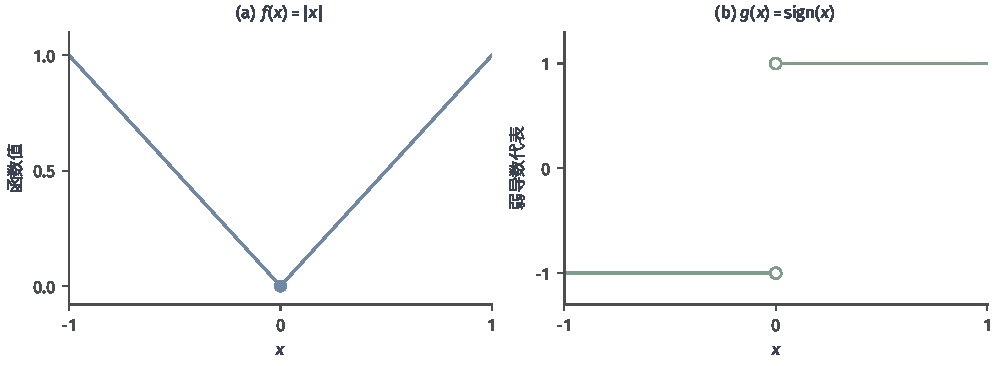
\includegraphics[width=169mm]{figures/01-mathematical-preliminaries-upper/02-linear-algebra-and-geometry/matplotlib/concepts-analysis-functional/weak-derivative.pdf}
 \functionalinlinefigurecaption{fig:functional-weak-derivative}
   {$f(x)=|x|$与其一阶弱导数$g(x)=\operatorname{sgn}(x)$。左图原点为连续尖点；右图两段分别为$-1$与$1$，空心端点表示经典导数在原点未定义。弱导数在原点的代表值可以任取，积分恒等式不受影响。}
\end{minipage}
\end{fullwidth}

\subsection{Sobolev空间}
\label{subsec:sobolev-spaces}

普通弱导存在还没有控制函数及导数的整体大小。本小节把规定阶弱导与原函数一起纳入范数，先确定成员与微分的定义域，再证明极限中的导数仍属于同一个函数；$p=2$的内积结构与$p=\infty$的补充范围分别标明。

\subsubsection{函数与弱导的共同积分控制}
\label{subsubsec:sobolev-members-norm}

\paragraph{$W^{k,p}$的成员与范数}

固定开域$\Omega\subset\mathbb R^d$、整数$k\ge0$及$1\le p<\infty$。为了同时控制函数偏差与规定阶的变化量，定义$W^{k,p}(\Omega)$由这样的$u$构成：
\[
  u\in L^p(\Omega),\qquad D^\alpha u\in L^p(\Omega)\quad(|\alpha|\le k),
\]
其中$D^0u=u$。局部可积性由$L^p$在紧集上的Hölder控制取得，因此这些弱导恒等式都有意义。

在这些等价类上定义
\begin{equation}
  \|u\|_{W^{k,p}}
  =\left(\sum_{|\alpha|\le k}\|D^\alpha u\|_p^p\right)^{1/p}.
  \label{eq:functional-sobolev-norm}
\end{equation}
零阶项控制函数本身，其余项控制各规定阶的变化量。有限个$L^p$分量的线性、正定与Minkowski不等式保证这是一个范数；只累计某一阶导数通常无法区分常数等零方向，不能不另作处理就替代当前全范数。

在有限区间$(-1,1)$上回用绝对值的弱导计算：函数和符号函数都属于每个有限$p$的$L^p$，故$|x|\in W^{1,p}(-1,1)$。阶跃虽属于该区间的$L^p$，但它的一阶分布导数是Dirac、没有普通局部可积表示，因此不属于$W^{1,p}$。这里用成员判定承接前例，不重复分部积分过程。

\paragraph{弱微分的定义域与误差控制}

对$|\alpha|\le k$，把弱微分看成映射
\[
  D^\alpha:W^{k,p}(\Omega)\to L^p(\Omega),
\]
由范数中包含该项直接得到
\[
  \|D^\alpha u\|_p\le\|u\|_{W^{k,p}}.
\]
相减后同样得到$\|D^\alpha(u-v)\|_p\le\|u-v\|_{W^{k,p}}$，因此这是在指定输入范数和定义域下的有界线性操作。

但这项控制不能被改写成“微分在任意$L^p\to L^p$上都有界”：普通$L^p$成员未必有该阶弱导，即使有导数，也没有这里的共同范数控制。输出仍是体内的弱导等价类，域内点值与整条边界记录要由后面的点值与边界读取按其输出类型另建条件。

\subsubsection{Sobolev空间的完备性}
\label{subsubsec:sobolev-completeness}

\paragraph{分量极限与弱导恒等式}

取$W^{k,p}$柯西列$(u_n)$。因为每一分量范数都不超过全范数，
\[
  \|D^\alpha u_n-D^\alpha u_m\|_p\le\|u_n-u_m\|_{W^{k,p}},
\]
故$(D^\alpha u_n)$对每个$|\alpha|\le k$都是$L^p$柯西列。回用已证明的$L^p$完备性，取得各分量极限
\[
  u_n\to v_0,\qquad D^\alpha u_n\to v_\alpha.
\]
此时它们还只是一组$L^p$元素，尚未证明彼此有导数关系。

固定$\varphi\in C_c^\infty(\Omega)$，对每个$n$写
\[
  \int_\Omega D^\alpha u_n\,\varphi\,\mathrm dx
  =(-1)^{|\alpha|}\int_\Omega u_nD^\alpha\varphi\,\mathrm dx.
\]
若$1<p<\infty$，用共轭指数$q$估计两侧差积分，分别不超过
\[
\begin{aligned}
  \left|\int(D^\alpha u_n-v_\alpha)\varphi\,\mathrm dx\right|
  &\le\|D^\alpha u_n-v_\alpha\|_p\,\|\varphi\|_q,\\
  \left|\int(u_n-v_0)D^\alpha\varphi\,\mathrm dx\right|
  &\le\|u_n-v_0\|_p\,\|D^\alpha\varphi\|_q;
\end{aligned}
\]
测试光滑且紧支撑，保证$\varphi$与$D^\alpha\varphi$在有限测度支撑上有界，两个$q$范数有限，两式右端随$n\to\infty$趋零。$p=1$时则分别以测试函数及其导数的上确界乘$L^1$误差，完成同样的极限传递。于是对所有测试都有
\[
  \int_\Omega v_\alpha\varphi\,\mathrm dx
  =(-1)^{|\alpha|}\int_\Omega v_0D^\alpha\varphi\,\mathrm dx.
\]
正是弱导定义把原本独立取得的各分量重新联系为同一个$v_0$的弱导$v_\alpha=D^\alpha v_0$，而不是仅凭记号称$v_\alpha$为导数。

各$v_\alpha$都属于$L^p$，因此$v_0\in W^{k,p}$；有限个分量的$L^p$误差都趋零，再相加开$p$次根，
\[
  \|u_n-v_0\|_{W^{k,p}}^p
  =\sum_{|\alpha|\le k}\|D^\alpha u_n-v_\alpha\|_p^p\longrightarrow0,
\]
便得到$u_n\to v_0$的Sobolev范数收敛。这样对有限$1\le p<\infty$完成了Banach性质；过程中没有要求边界光滑，也没有推出逐点或边界读取。

\paragraph{$H^k$的Hilbert结构}

固定$p=2$并记$H^k(\Omega)=W^{k,2}(\Omega)$，定义
\[
  \langle u,v\rangle_{H^k}
  =\sum_{|\alpha|\le k}\int D^\alpha u\,D^\alpha v.
\]
各项积分存在、双线性和对称性由$L^2$内积继承，零阶项保证正定，诱导范数正是上面选定的$W^{k,2}$范数。前一单元已经证明该范数下完备，现在才能称$H^k$为Hilbert空间；不能只把多个内积相加，就省略“极限中导数关系”的核验。后面的正交分解与函数目标可据此使用Hilbert工具，具体点值、边界迹和零边界闭包仍在位置读取一节处理。

\subsubsection{本质上界控制的补充范围}
\label{subsubsec:sobolev-infty-supplement}

若还要允许$p=\infty$，可另定义$W^{k,\infty}(\Omega)$，要求$u$及规定阶普通弱导都属于$L^\infty$，并采用
\[
  \max_{|\alpha|\le k}\|D^\alpha u\|_\infty.
\]
这是本质最大控制的共同范数，不把$\sum\|D^\alpha u\|_p^p$直接代入无穷指数，也不把这一补充推广写成正文已经完成的结论。其完备性若展开，仍可沿用“分量极限—测试恒等式—原空间极限”的同一路线，但改用$L^\infty$完备性，并以本质上界误差乘测试函数（或其导数）的$L^1$范数传递积分。这里只标清它与有限$p$论证相同的职责和不同的估计；正文后续主要使用$H^1$，不另行扩展一般嵌入定理或迹定理。
\section{函数的线性读取与正交表示}
\label{sec:linear-readouts-orthogonal}

前面把函数空间本身作为对象，建立了$L^2$范数、弱导与Sobolev空间。本节固定一个已经选定的实Hilbert函数空间$H$，研究两类具体读取：把函数映成标量的线性读数，以及把函数分解成一组正交方向上的记录。有限维线性代数中，最近分量、坐标变换和点值都是熟悉操作；无限维时，下确界是否达到、读数是否被范数控制、记录是否完备，都必须重新逐条检验。闭子空间投影与有界线性泛函表示是后面所有系数记录和位置记录的共同工具，先一并建立。

\subsection{有界线性泛函的表示}
\label{subsec:bounded-functional-representation}

先证明闭子空间确有最近分量，再把有界标量读数表示为内积中的一个固定方向。两者是工具与其应用的关系：投影先用来研究表示，随后又被正交展开反复调用。

\subsubsection{闭子空间的正交投影}
\label{subsubsec:orthogonal-projection}

\paragraph{最近分量的存在与正交性}

固定实Hilbert空间$H$、闭线性子空间$M\subset H$及$f\in H$，记
\[
d=\inf_{u\in M}\|f-u\|.
\]
距离是下确界，事先并不保证有$u\in M$达到它。下面的定理把存在性、正交特征和唯一性一次建立起来。

\begin{theorem}[正交投影]
\label{thm:orthogonal-projection}
设$H$为实Hilbert空间，$M\subset H$为闭线性子空间，$f\in H$。则存在唯一的$p\in M$使$\|f-p\|=d$，且该$p$满足$f-p\perp M$；反之，任何$p\in M$满足$f-p\perp M$都达到这一下确界。
\end{theorem}

\begin{proof}
取极小化列$u_n\in M$使$\|f-u_n\|\to d$。对任意$n,k$，因$(u_n+u_k)/2\in M$，由定义$\|f-(u_n+u_k)/2\|\ge d$。平行四边形恒等式给出
\[
\|(f-u_n)+(f-u_k)\|^2+\|(f-u_n)-(f-u_k)\|^2
=2\|f-u_n\|^2+2\|f-u_k\|^2.
\]
左端第一项等于$4\|f-(u_n+u_k)/2\|^2\ge 4d^2$，左端第二项正是$\|u_n-u_k\|^2$，故
\[
\|u_n-u_k\|^2\le 2\|f-u_n\|^2+2\|f-u_k\|^2-4d^2\longrightarrow0.
\]
$(u_n)$因而为Cauchy列。$H$完备，$u_n\to p\in H$；$M$闭，故$p\in M$；范数连续给出$\|f-p\|=d$，存在性成立。

再证正交性。任取$h\in M$和实数$t$，$p+th\in M$，故
\[
\|f-p-th\|^2\ge d^2=\|f-p\|^2.
\]
展开左端：$\|f-p\|^2-2t\langle f-p,h\rangle+t^2\|h\|^2$。这是关于$t$的二次函数，在$t=0$处取得最小值；因$M$是线性空间，$t$可正可负，两侧导数都允许，故一次项系数必须为零：$\langle f-p,h\rangle=0$。由$h$任意，$f-p\perp M$。

最后证唯一性与反向刻画。若$p\in M$且$f-p\perp M$，则对任意$u\in M$，$p-u\in M$，于是
\[
\|f-u\|^2=\|f-p\|^2+\|p-u\|^2\ge\|f-p\|^2,
\]
等号当且仅当$u=p$。既达到下确界的$p$唯一，又满足正交性；已证存在的$p$也满足同一分解，两个角色由同一元素担任。
\end{proof}

记$p=P_Mf$，称为$f$在$M$上的\term{正交投影}。由唯一分解$f=P_Mf+(f-P_Mf)$，其中$P_Mf\in M$而$f-P_Mf\in M^\perp$，可得$P_M$线性：对$af+bg$，$aP_Mf+bP_Mg\in M$，其余量$a(f-P_Mf)+b(g-P_Mg)\in M^\perp$，由分解唯一即等于$P_M(af+bg)$。又
\begin{equation}
\label{eq:functional-projection-error-decomposition}
\|f\|^2=\|P_Mf\|^2+\|f-P_Mf\|^2,
\end{equation}
故$\|P_Mf\|\le\|f\|$；投影作为线性算子的误差传播统一放在算子框架中讨论。

\paragraph{闭性与完备性各自保障哪一步}

上面证明的两步桥梁不能省去：极小化列成为Cauchy列靠平行四边形恒等式，极限留在$M$内靠$M$闭，极限存在靠$H$完备。三者缺一会出什么问题，用一个具体例子看清楚。

在$L^2([0,1],\mathrm dx)$中取阶跃$q=\mathbb I_{(1/2,1]}$，令连续函数
\[
u_n(t)=
\begin{cases}
0,&t\le1/2,\\
n(t-1/2),&1/2<t<1/2+1/n,\\
1,&t\ge1/2+1/n.
\end{cases}
\]
$u_n$连续，且与$q$只在$(1/2,1/2+1/n)$上相差$1-n(t-1/2)$，直接积分
\[
\|u_n-q\|_2^2=\int_{1/2}^{1/2+1/n}(1-n(t-1/2))^2\,\mathrm dt=\frac1{3n}\to0.
\]
但$q$的$L^2$等价类没有任何连续代表：连续函数在一点的值决定其在一个邻域上的值，而$q$在$1/2$两侧本质不同。于是连续函数构成的集合$C([0,1])$在$L^2$中不闭：极限$q$离开了该集合。反过来，若把环境取为$C([0,1])$并配$L^2$范数，该空间又不完备：$(u_n)$在$L^2$范数下是Cauchy列，却不在$C([0,1])$中有极限。闭性保障“极限留在可行集内”，完备性保障“环境中有极限可取”，两件事不能合并成一句“无限维中自然成立”。

\begin{figure}[h]
  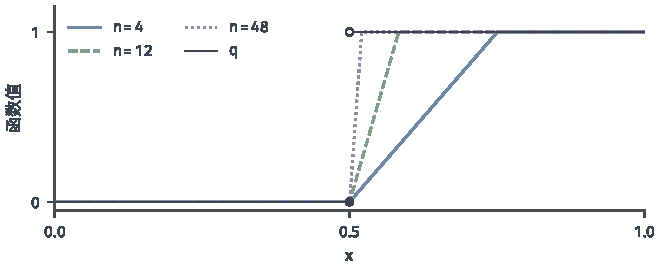
\includegraphics[width=112mm]{figures/01-mathematical-preliminaries-upper/02-linear-algebra-and-geometry/matplotlib/comprehension-additions/functional-incomplete-continuous.pdf}
  \caption{连续斜坡$u_n(t)=\operatorname{clip}(n(t-1/2),0,1)$取$n=4,12,48$（实、虚、点线），灰黑阶跃为$q=\mathbb I\{t>1/2\}$。黑实点与空心圈标明阶跃在$1/2$处的取值；斜坡逐点趋于阶跃，但$\|u_n-q\|_2^2=1/(3n)\to0$，$u_n$在一致范数下并不收敛到任何连续函数。图说明$C([0,1])$在$L^2$范数下不闭，不表示该阶跃有连续代表。}
  \label{fig:vol1-add-functional-incomplete-continuous}
\end{figure}

后面Riesz表示对闭零空间使用这条投影；正交系数对有限方向的张成使用这条投影。一般闭凸集合上的最近点涉及变分不等式，留给函数值拟合任务处理，因为那里改变的是可行集合，而非线性记录方向。

\subsubsection{有界线性泛函与Riesz表示}
\label{subsubsec:riesz-representation}

\paragraph{标量读取与有界性}

固定实Hilbert空间$H$，映射$L:H\to\mathbb R$称为\term{线性泛函}，若
\[
L(af+bg)=aL(f)+bL(g)\qquad(\forall f,g\in H,\ a,b\in\mathbb R).
\]
它把一个函数读成一个标量。若存在与$f$无关的常数$C$使
\[
|L(f)|\le C\|f\|\qquad(\forall f\in H),
\]
则称$L$有界，并定义最佳常数
\[
\|L\|=\sup_{\|f\|\le1}|L(f)|.
\]
有界性是“单位球上的输出有统一界”，与某个具体$f$的输出数值有限不是同一回事。

每个固定方向$h\in H$都给出一个有界读取$L_h(f)=\langle f,h\rangle_H$：由Cauchy–Schwarz，$|L_h(f)|\le\|h\|\|f\|$，故$\|L_h\|\le\|h\|$；取$f=h/\|h\|$（$h\ne0$）时$L_h(f)=\|h\|$，反向不等式成立，$\|L_h\|=\|h\|$。自然的反向问题是：每一个有界线性读取是否都来自某个固定方向？下面的Riesz表示给出肯定回答。

\paragraph{由零空间投影证明表示}

\begin{theorem}[Riesz表示]
\label{thm:riesz}
设$H$为实Hilbert空间，$L:H\to\mathbb R$为有界线性泛函。则存在唯一的$h_L\in H$，使
\begin{equation}
\label{eq:functional-riesz-representation}
L(f)=\langle f,h_L\rangle_H\qquad(\forall f\in H),
\end{equation}
且$\|L\|=\|h_L\|_H$。
\end{theorem}

\begin{proof}
若$L=0$，取$h_L=0$即可。下设$L\ne0$。

零空间$N=\{f\in H:L(f)=0\}$是$H$的线性子空间。它闭：若$f_n\in N$且$f_n\to f$，由有界性$|L(f)|=|L(f)-L(f_n)|\le\|L\|\|f-f_n\|\to0$，故$f\in N$。

取$v\in H$使$L(v)\ne0$。设$v=p+w$为$v$在$N$上的正交投影分解：$p=P_Nv\in N$，$w=v-p\perp N$。由$L(w)=L(v)-L(p)=L(v)\ne0$知$w\ne0$。

对任意$f\in H$，构造
\[
f-\frac{L(f)}{L(w)}\,w.
\]
它在$L$下的像为$L(f)-\frac{L(f)}{L(w)}L(w)=0$，故属于$N$；而$w\perp N$，与$w$取内积得零：
\[
\langle f,w\rangle-\frac{L(f)}{L(w)}\|w\|^2=0,
\qquad\text{即}\qquad
\langle f,w\rangle=\frac{L(f)}{L(w)}\|w\|^2.
\]
令
\begin{equation}
\label{eq:functional-riesz-direction}
h_L=\frac{L(w)}{\|w\|^2}\,w,
\end{equation}
则$L(f)=\langle f,w\rangle\,L(w)/\|w\|^2=\langle f,h_L\rangle$，表示成立。

唯一性：若$h,h'$都满足$L(f)=\langle f,h\rangle=\langle f,h'\rangle$，则$\langle f,h-h'\rangle=0$对一切$f$成立；取$f=h-h'$得$\|h-h'\|^2=0$。

范数等式：由$|L(f)|\le\|h_L\|\|f\|$得$\|L\|\le\|h_L\|$。反向，$L(h_L)=\langle h_L,h_L\rangle=\|h_L\|^2$，故$\|h_L\|=|L(h_L)|/\|h_L\|\le\|L\|$。两端相等。
\end{proof}

表示结论只适用于已经有界的标量泛函。它不能事先证明任意点读数有界——那要在点值一节单独检验；也不能把输出为整条边界函数的迹算子缩成单个内积方向，因为迹的输出不是标量。有界性、标量输出、Hilbert内积三者齐备，Riesz才给出一个方向。

\subsection{正交展开与系数记录}
\label{subsec:orthogonal-expansions-coefficients}

本小节固定表示方向，研究已知函数如何按正交方向分解、截断后丢失多少，以及不同有限记录之间如何转换。三个子题按同一记录任务的组成分工：建立方向记录、评估有限保留、转换记录坐标。

\subsubsection{正交系数与函数展开}
\label{subsubsec:orthogonal-records}

\paragraph{正交方向与完整记录}

设$H$为实Hilbert空间，序列$(e_j)_{j\ge1}\subset H$满足
\[
\langle e_j,e_k\rangle_H=\delta_{jk}.
\]
称$(e_j)$为正交归一序列；若所有有限线性组合在$H$中稠密，即$\overline{\operatorname{span}}\{e_j\}=H$，则称它为$H$的\term{完备正交系}（也叫正交归一基）。环境空间完备不等于所选正交系覆盖全部方向：在$\ell^2$中取仅偶数坐标非零的方向$e_2,e_4,\dots$，它们正交归一，其闭张成是$\ell^2$的真闭子空间，奇数方向整个缺失。

对前$m$个方向的张成$S_m=\operatorname{span}\{e_1,\dots,e_m\}$使用正交投影定理。$S_m$有限维因而闭。记$c_j=\langle f,e_j\rangle$，则
\begin{equation}
\label{eq:functional-orthogonal-partial-projection}
P_{S_m}f=\sum_{j=1}^m c_j e_j.
\end{equation}
验证：右端属于$S_m$，且对每个$k\le m$，$f-\sum_{j\le m}c_je_j$与$e_k$的内积为$c_k-c_k=0$，故与整个$S_m$正交。每个系数$c_j$正是前一小节$h_L=e_j$时的有界标量读取，$|c_j|\le\|f\|$。

正交性给出逐项相消的误差：
\begin{equation}
\label{eq:functional-bessel}
\|f-P_{S_m}f\|^2=\|f\|^2-\sum_{j=1}^m|c_j|^2,
\end{equation}
因而Bessel不等式$\sum_{j=1}^m|c_j|^2\le\|f\|^2$对一切$m$成立，正项级数$\sum_j|c_j|^2$收敛且不超过$\|f\|^2$。

\begin{theorem}[完备正交系与Parseval等式]
\label{thm:parseval}
设$(e_j)$为$H$的完备正交系，$c_j=\langle f,e_j\rangle$。则
\[
\begin{aligned}
\lim_{m\to\infty}\|f-\sum_{j=1}^m c_je_j\|=0,
\qquad
\|f\|^2=\sum_{j=1}^\infty|c_j|^2,\\
f=\sum_{j=1}^\infty c_je_j\quad(\text{依}H\text{范数}).
\end{aligned}
\]
\end{theorem}

\begin{proof}
记$s_m=\sum_{j\le m}c_je_j=P_{S_m}f$。由$S_m$张成在$H$中稠密，对$\varepsilon>0$存在有限组合$u=\sum_{j\le m_0}a_je_j$使$\|f-u\|<\varepsilon$。$s_{m_0}$是$f$在$S_{m_0}$上的最佳逼近，故$\|f-s_{m_0}\|\le\|f-u\|<\varepsilon$；而由Bessel误差公式，$\|f-s_m\|^2$随$m$增大单调不增（尾余项为正项级数尾和），故对一切$m\ge m_0$，$\|f-s_m\|<\varepsilon$。范数展开与Parseval等式随之成立。
\end{proof}

若正交系不完备，$P_{S_m}f$只收敛到$f$在其闭张成上的投影，正交余部$\overline{\operatorname{span}}\{e_j\}^\perp$中的分量永远保留。Bessel不等式与Parseval等式的差别正是覆盖条件的差别，不能混用。

\paragraph{傅里叶方向的计算与遗漏}

在$L^2([-\pi,\pi],\mathrm dx)$中取\term{傅里叶基}，即
\[
e_0=\frac1{\sqrt{2\pi}},\qquad
e_j^c=\frac{\cos(jx)}{\sqrt\pi},\qquad
e_j^s=\frac{\sin(jx)}{\sqrt\pi}\quad(j\ge1).
\]
直接积分给出
\[
\begin{aligned}
\int_{-\pi}^{\pi}\cos(jx)\cos(kx)\,\mathrm dx=\pi\delta_{jk},
\qquad
\int_{-\pi}^{\pi}\sin(jx)\sin(kx)\,\mathrm dx=\pi\delta_{jk},\\
\int_{-\pi}^{\pi}\cos(jx)\sin(kx)\,\mathrm dx=0.
\end{aligned}
\]
它们构成正交归一系；经典三角级数理论给出其完备性。正交评估的是函数内积：例如$1$与$x$的乘积在正负半区间相消，不等于“平面图像互相垂直”这种几何画面。

取$f(x)=x$。$f$是奇函数，故常数项与全部余弦系数为零。对第一个正弦方向分部积分：
\[
\begin{aligned}
\int_{-\pi}^{\pi}x\sin x\,\mathrm dx
&=\bigl[-x\cos x\bigr]_{-\pi}^{\pi}+\int_{-\pi}^{\pi}\cos x\,\mathrm dx\\
&=-\pi(-1)+\pi(-1)\cdot(-1)+0=2\pi,
\end{aligned}
\]
故第一个正弦系数为
\[
\frac1{\sqrt\pi}\int_{-\pi}^{\pi}x\sin x\,\mathrm dx=2\sqrt\pi.
\]
一般地，$\frac1{\sqrt\pi}\int_{-\pi}^{\pi}x\sin(jx)\,\mathrm dx=2\sqrt\pi\,(-1)^{j+1}/j$。Parseval等式此时成为可复算的检验：
\[
\sum_{j=1}^\infty\frac{4\pi}{j^2}=\frac{2\pi^3}{3}=\int_{-\pi}^{\pi}x^2\,\mathrm dx,
\]
其中$\sum_j1/j^2=\pi^2/6$。

保留常数及前$m$组正弦、余弦即得傅里叶截断。只取余弦方向时投影恒为零，增加再多同类方向也不能逼近$x$——方向选错时数量不补覆盖。完整三角系在上述$L^2$范数下完备，但范数收敛不自动承诺逐点收敛或一致收敛；截断误差在下一小节专门计算。

\subsubsection{正交截断与尾误差}
\label{subsubsec:truncation-tail}

固定同一$f$与同一完备正交系，只改变保留项数$m$，$s_m=\sum_{j\le m}c_je_j$是一个函数序列。由上节误差公式，
\begin{equation}
\label{eq:functional-truncation-tail}
\|f-s_m\|^2=\sum_{j>m}|c_j|^2\longrightarrow0,
\end{equation}
收敛来自可求和级数$\sum_j|c_j|^2$的尾部消失。每个$s_m$在当前前$m$个方向内最佳，但这并未与所有同规模非线性表示作比较——表示方向怎样选择由有限表示任务处理，这里固定方向后只回答截断是否收敛。

式\eqref{eq:functional-truncation-tail}只控制所选空间范数。点值误差要等点值读取建立相应有界常数后才能传递；一致误差还要求对所有位置有统一的读取界。不能从$L^2$尾项直接跳到逐点或一致收敛。另外，积分谱中的$L^2$归一方向与核RKHS中的归一方向尺度不同，相应的两种尾误差在Mercer展开处分别给出，此处不提前引入尚未定义的权重。

\subsubsection{系数与有限读数的转换}
\label{subsubsec:record-conversion}

\paragraph{换基与记录矩阵}

先限定$f=\sum_{j=1}^m a_j\varphi_j$属于已知有限维张成。线性无关的方向使系数由函数唯一确定；方向相关时，不同系数组可表示同一函数；一般非线性参数族则不能套用线性基的结论。

对$f(t)=a+bt$，把基$(1,t)$改为$(1,t-c)$，逐项展开
\[
f(t)=a+bt=(a+bc)+b(t-c),
\]
新系数为$(a+bc,b)$。这只改变记录坐标，目标函数及其取值完全相同。改读$f(0),f(1)$时，
\[
\begin{pmatrix}f(0)\\f(1)\end{pmatrix}
=\begin{pmatrix}1&0\\1&1\end{pmatrix}\begin{pmatrix}a\\b\end{pmatrix},
\]
由$f(0)=a$、$f(1)-f(0)=b$恢复系数。若只读$f(0)$，斜率方向不可见：可逆矩阵与缺失列分别意味着记录完整与方向丢失。

对一般线性读数$L_i$（$i=1,\dots,n$），记录矩阵$A\in\mathbb R^{n\times m}$的第$(i,j)$项为
\[
A_{ij}=L_i(\varphi_j).
\]
点值读数给出$A_{ij}=\varphi_j(x_i)$，积分读数给出$A_{ij}=\int\varphi_j w_i\,\mathrm d\mu$。代入前须核对定义域、积分存在与输出类型，再执行矩阵换算$L(f)=Aa$。

\paragraph{有限表示之外的边界}

矩阵可逆只说明：在指定的有限维候选张成内部，记录与系数的转换唯一。若候选扩大到任意函数，同样$n$条读数可能对应无穷多个函数——这是新增的单射性问题，交给有限读数的可识别性任务，不在已知表示的换算中提前宣告恢复成功。无限表示还须指定收敛范数、尾误差和极限归属；上面的正交截断提供了一种可核验情形，其他表示按各自条件判断，不能把有限求和矩阵原样当成无限展开的计算保证。

\subsection{点值与边界读取}
\label{subsubsec:point-boundary-readouts}

本小节按输出位置区分单点取值与整条边界记录。前者输出标量，后者通常输出边界函数等价类。共同要求是：先明确输入元素和合法代表，再判断读取是否存在并受范数控制。

\subsubsection{域内点值读取}
\label{subsubsec:point-evaluation}

\paragraph{等价类与合法代表}

在通常Lebesgue测度的$[0,1]$上，零函数与仅在$x=1/2$取$1$的函数是同一个$L^2$元素，却给出不同的点值。因此任取一个可测代表再读取该点，不能在商空间上定义同一个数：点值读取首先不是“是否有界”，而是“在等价类上是否良定义”。

该反例依赖单点的可测性与零测度。若$\mu(\{x\})>0$，两个几乎处处相等的代表在$x$处必相等，且有限$p$时
\[
|f(x)|\le\mu(\{x\})^{-1/p}\|f\|_p,
\]
正质量单点要另作判断，不能把零测点的结论推广到所有测度。

若某等价类存在连续代表，且测度在定义域上全支撑，则这样的代表唯一：两个连续代表若在一点不同，差异会延伸到一个正测度邻域，与几乎处处相等矛盾。这里解决的是唯一性；代表是否存在仍需额外正则性结论。若输入本来就是真实连续函数，或已由条件选出唯一连续代表，点读数有确定含义，但这个数是否被当前范数控制仍未解决。

\paragraph{点值的有界性与维数条件}

对已经良定义的线性点读数$L_x(f)=f(x)$，提出有界性要求
\[
|L_x(f)|\le C_x\|f\|,
\]
其中$C_x$可依赖位置$x$，但不能依赖$f$。在$[0,1]$上取连续尖峰
\[
f_n(t)=\max(1-nt,0),
\]
直接算得$\|f_n\|_2^2=\int_0^{1/n}(1-nt)^2\mathrm dt=1/(3n)$，而$f_n(0)=1$，比值$\sqrt{3n}$无界。故连续函数上的$L^2$范数不能控制原点读取；零点是闭区间中允许的输入位置，此例不替代一般区域的边界迹定理。

与积分读取对照：$L_w(f)=\int fw\,\mathrm d\mu$在$w\in L^2$时由Cauchy–Schwarz给出$|L_w(f)|\le\|w\|_2\|f\|_2$；正交系数也是这类内积读取。问题出在点读数与所选范数的组合，而非线性读取本身。

在一维有界区间$I=(a,b)$上，Sobolev范数确实控制点值，下面把这件事完整做完。设$u\in H^1(I)$，弱导$g\in L^2(I)$。令
\[
F(x)=\int_a^x g(t)\,\mathrm dt.
\]
积分基本定理给出$F$绝对连续；分部积分核对其弱导为$g$，故$u-F$的分布导数为零。要得到$u$的点值，还须说明零分布导数迫使$u-F$为常数。

设$T_{u-F}$为$u-F$诱导的分布。先取积分为零的紧支撑光滑测试$\psi$：其积分原函数$\varphi(x)=\int_a^x\psi$仍紧支撑且$\varphi'=\psi$，由$u-F$分布导数为零得
\[
0=\int(u-F)\varphi'=\int(u-F)\psi.
\]
固定一个积分为$1$的测试$\rho$。任意测试$\psi$可分解为$(\int\psi)\rho+\bigl(\psi-(\int\psi)\rho\bigr)$，第二项积分为零，被上式灭掉；于是
\[
T_{u-F}(\psi)=c\int\psi,\qquad c=T_{u-F}(\rho).
\]
即分布$T_{u-F}$等于常数$c$作为普通函数的分布。由普通函数表示分布的唯一性，$u-F=c$几乎处处。于是$c+F$是$u$的绝对连续代表，其每一点值合法且唯一。

记区间长度$L=b-a$。由平方积分平均，存在$y\in I$使
\[
|u(y)|\le L^{-1/2}\|u\|_2.
\]
对闭区间中任意$x$，$u(x)-u(y)=\int_y^x g$，再用Cauchy–Schwarz，
\begin{equation}
\label{eq:functional-point-evaluation-embed}
|u(x)|\le L^{-1/2}\|u\|_2+L^{1/2}\|g\|_2.
\end{equation}
该估计对闭区间中的$x$统一成立：一维$H^1$既解决单点有界，也给出全域控制。

一维结论不能跨维照搬。在三维域内部固定$x_0$，取光滑紧支撑$\varphi$且$\varphi(0)=1$，令$f_n(x)=\varphi(n(x-x_0))$，$n$足够大时支撑在域内。换元给出
\[
\|f_n\|_2^2=n^{-3}\|\varphi\|_2^2,\qquad
\|\nabla f_n\|_2^2=n^{-1}\|\nabla\varphi\|_2^2,\qquad
f_n(x_0)=1.
\]
于是$f_n(x_0)/\|f_n\|_{H^1}\asymp n^{1/2}\to\infty$：即使限制光滑函数，三维$H^1$范数也不能控制该点读数。一般逐点常数$C_x$可随位置增长，只有$\sup_xC_x<\infty$才给统一控制。取整条实轴上由$f(t)=bt$组成、范数为$|b|$的函数空间，点读数常数恰为$|x|$；真正把输入域限制为$[-3,3]$，才能取得统一常数$3$——图\ref{fig:vol1-add-functional-pointwise-bound-growth}同时画出两条单位范数函数与逐点常数，注意显示窗口不是定义域，$C_x$在实轴上无界。

\begin{figure}[h]
  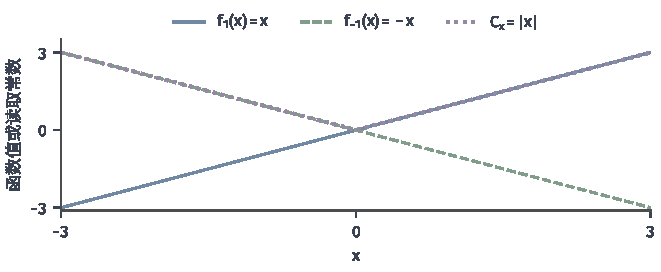
\includegraphics[width=112mm]{figures/01-mathematical-preliminaries-upper/02-linear-algebra-and-geometry/matplotlib/comprehension-additions/functional-pointwise-bound-growth.pdf}
  \caption{在$H=\{f(t)=bt\}$、$\|f\|_H=|b|$的空间中，单位范数函数$f_1(t)=t$与$f_{-1}(t)=-t$（实、虚线），点$x$处的最佳读取常数$C_x=|x|$（点线）。$x$离原点越远，同样范数函数在该点的值越大；在整条实轴上$C_x$无界，统一读取界不存在。显示窗口$[-3,3]$不是输入域。}
  \label{fig:vol1-add-functional-pointwise-bound-growth}
\end{figure}

\paragraph{再生核Hilbert空间与正向表示}

在真实函数组成的实Hilbert空间$H$中，把每个点读数$L_x:f\mapsto f(x)$都有界作为空间条件，称这样的空间为\term{再生核Hilbert空间}（RKHS）。先有点读数有界，才能调用Riesz表示取得唯一$K_x\in H$使
\begin{equation}
\label{eq:functional-reproducing-property}
f(x)=\langle f,K_x\rangle_H\qquad(\forall f\in H).
\end{equation}
定义$K(x,z)=K_z(x)=\langle K_z,K_x\rangle_H$，称它为$H$的\term{再生核}。由内积对称性，$K(x,z)=K(z,x)$；对任意有限点组与系数，
\[
0\le\Big\|\sum_i a_iK_{x_i}\Big\|_H^2
=\sum_{i,j}a_ia_jK(x_i,x_j),
\]
故核对称且Gram矩阵半正定；满足这条Gram半正定性的$K$称为\term{正定核}。$K:X\times X\to\mathbb R$是标量核。

由Riesz最佳常数，
\begin{equation}
\label{eq:functional-rkhs-pointwise-bound}
\|L_x\|=\|K_x\|_H=\sqrt{K(x,x)}.
\end{equation}
核对角上界$K(x,x)\le M^2$才使同一个$M$控制所有点：这解释了何种空间结构支持统一读取。

固定仿射核$K(x,z)=1+xz$，令
\[
H=\{f(t)=a+bt\},\qquad
\langle a+bt,a'+b't\rangle_H=aa'+bb'.
\]
取$K_x(t)=1+xt$，逐项核对：
\[
\langle a+bt,K_x\rangle_H=a\cdot1+b\cdot x=a+bx=f(x),
\]
$\|f\|_H^2=a^2+b^2$，$\|K_x\|_H^2=1+x^2$。抽象的再生关系在这里有完整坐标计算。

\paragraph{由半正定核反向构造空间}

正向构造从空间出发得到核；反过来，固定非空集合$X$与实对称半正定核$K$，也能唯一造出以$K$为再生核的RKHS。

先用有限核截面的形式线性组合建立双线性型
\[
\Big\langle\sum_i a_iK_{x_i},\sum_jb_jK_{z_j}\Big\rangle
=\sum_{i,j}a_ib_jK(x_i,z_j).
\]
Gram二次型半正定只给出半内积：存在非零组合长度为零。半内积的Cauchy–Schwarz$|\langle f,g\rangle|\le\|f\|\|g\|$表明，零长度方向在每点读数均为零，并有
\[
|f(x)|=|\langle f,K_x\rangle|\le\sqrt{K(x,x)}\,\|f\|.
\]
因此先商去零长度方向，读取在商空间上良定义，不能直接声称半内积空间已是Hilbert空间。

对该内积空间作完备化。逐点读取界使每条Cauchy列在每个$x$处取得确定极限（$|f_n(x)-f_m(x)|\le\sqrt{K(x,x)}\|f_n-f_m\|$），并使等价Cauchy列定义同一函数。若完成后的元素在所有点为零，它与每个$K_x$正交；核截面张成稠密，故该元素为零——完备化到函数空间的表示因此单射。核截面内积与再生关系在极限下保留，得到以$K$为再生核的RKHS。任何其他同核RKHS在核截面张成上内积相同，由稠密性唯一延拓，故空间由核唯一确定。半正定允许有限Gram矩阵奇异，不能把“正定核”的常用约定误读为所有Gram矩阵严格正定。

这条构造只需集合与半正定核，不需事先给测度。后面的积分谱还要另给测度及连续性、紧性条件；RKHS是具有稳定点读数的Hilbert函数空间，不是与Hilbert空间或Banach空间互斥的类别。

\paragraph{固定点的函数误差与位置误差}

先固定$x$和核空间，仅把$f$改为$f+h$。由再生关系，
\begin{equation}
\label{eq:functional-rkhs-error-fixedpoint}
|(f+h)(x)-f(x)|=|\langle h,K_x\rangle_H|
\le\sqrt{K(x,x)}\,\|h\|_H.
\end{equation}
这是有界读取在固定点的应用。再固定同一$f$，只把位置$x$改为$z$：
\[
f(x)-f(z)=\langle f,K_x-K_z\rangle_H,
\]
故
\[
\begin{aligned}
|f(x)-f(z)|\le\|f\|_H\|K_x-K_z\|_H,\\
\|K_x-K_z\|_H^2=K(x,x)+K(z,z)-2K(x,z).
\end{aligned}
\]
位置稳定取决于核截面在空间范数中的接近。若$X$有拓扑且$K$连续，上式给出核截面随位置连续，进而给出每个$f\in H$的连续性；若还要对一整类函数统一控制，则固定该类的范数半径。单点读取有界本身未包含位置连续性，两种扰动不能混成一项。

\subsubsection{边界迹与零边界空间}
\label{subsubsec:trace-zero-boundary}

弱导空间首先由体内几乎处处等价类组成；边界条件需要一条由体内元素到边界记录的合法映射，不能任取代表后逐点限制。

\paragraph{迹的输出与连续延拓}

固定有界Lipschitz区域$\Omega\subset\mathbb R^d$、边界表面测度$\mathrm dS$与输入空间$H^1(\Omega)$。所需输出是$L^2(\partial\Omega,\mathrm dS)$中的边界函数等价类，不是某个边界点上的标量，因而不是一个Riesz方向可以表示的对象。

在光滑函数上，限制$u\mapsto u|_{\partial\Omega}$就是熟悉的边界取值。把它延拓到整个$H^1(\Omega)$需要一个前提估计。标准迹定理指出：对上述Lipschitz区域，存在常数$C_\Omega$使
\begin{equation}
\label{eq:functional-trace-inequality}
\|u|_{\partial\Omega}\|_{L^2(\partial\Omega,\mathrm dS)}
\le C_\Omega\|u\|_{H^1(\Omega)}
\qquad(\forall u\in C^\infty(\overline\Omega)).
\end{equation}
其证明通过边界局部平直化，把问题化到半空间的一维论证（与本节端点估计同源），再用光滑逼近完成；一维区间上的端点估计式\eqref{eq:functional-point-evaluation-embed}是它最简单的特例，不能冒充一般区域的证明。

对任意$u\in H^1(\Omega)$，取光滑逼近列$u_n\in C^\infty(\overline\Omega)$在$H^1(\Omega)$中收敛于$u$。由式\eqref{eq:functional-trace-inequality}，
\[
\|u_n|_{\partial\Omega}-u_m|_{\partial\Omega}\|_{L^2(\partial\Omega)}
\le C_\Omega\|u_n-u_m\|_{H^1(\Omega)},
\]
故边界限制列在$L^2(\partial\Omega)$中为Cauchy列。$L^2$完备，取得极限；若另取逼近列$v_n\to u$，混合列$(u_1,v_1,u_2,v_2,\dots)$同样$H^1$收敛，其边界列极限唯一，故极限与逼近列选择无关。以此定义连续延拓
\[
\operatorname{Tr}:H^1(\Omega)\to L^2(\partial\Omega,\mathrm dS),
\]
并保留同一范数界$\|\operatorname{Tr}u\|_{L^2(\partial\Omega)}\le C_\Omega\|u\|_{H^1(\Omega)}$。迹算子是有界线性算子，其输出类型为边界函数等价类。

\paragraph{零迹与固定边界的可行集合}

用$H^1$范数闭包定义
\[
H_0^1(\Omega)=\overline{C_c^\infty(\Omega)}^{\,H^1(\Omega)},
\]
该定义不依赖任意代表的逐点边界值。由$\operatorname{Tr}$连续且$C_c^\infty(\Omega)$中函数在边界附近为零，$H_0^1\subseteq\ker\operatorname{Tr}$。标准零迹刻画定理给出反向包含：在上述Lipschitz区域条件下，$\ker\operatorname{Tr}$恰为$C_c^\infty(\Omega)$的$H^1$闭包，故
\[
H_0^1(\Omega)=\ker\operatorname{Tr}.
\]

迹的像不能直接当成全部$L^2$边界函数。若已知合法边界数据$g=\operatorname{Tr}G$，候选集合可写成$G+H_0^1(\Omega)$：允许扰动具有零迹。这为后面的梯度拟合提供不依赖点值代表的边界接口。自由边界则允许相应边界扰动；具体自然通量由变分任务及额外正则性推导，此处不提前给所有弱解定义普通法向导数。

\section{线性算子与积分方程}
\label{sec:linear-operators-integral-equations}

本节研究函数空间之间的线性运算及其方程：先建立各类运算共用的定义域、范数与算子性质，再对积分算子检查作用是否合法、怎样改变方向，最后求解该积分运算进入的方程。共用准备与两个主体任务分别标明，不能把一般算子性质藏在积分核的例子里，也不能把求解方程与已知函数的正向积分混成同一种输出。

\subsection{线性算子的共同框架}
\label{subsec:operator-framework}

本小节只建立后面确实使用的输入输出、误差范数、伴随与紧性语言。点读数和投影是已经见过的实例，微分与迹说明定义域和目标空间也可能改变。

\subsubsection{定义域、有界性与输入误差}
\label{subsubsec:operator-domain-boundedness}

\paragraph{线性算子及所用范数}

固定赋范空间$V,W$，映射$A:V\to W$称为线性算子，若
\[
A(af+bg)=aAf+bAg.
\]
若实际只允许定义域$D(A)\subset V$中的输入，应在一开始写清该线性定义域；函数、导数或积分存在的成员条件不能省略成一个形式公式。有界算子框架先取$A$在整个$V$上定义；若只取受限定义域，须另写其所赋范数，不自动调用全空间结论。

定义算子范数
\[
\|A\|_{\mathrm{op}}=\sup_{\|f\|_V\le1}\|Af\|_W.
\]
其有限等价于存在统一常数$C$使$\|Af\|_W\le C\|f\|_V$，最佳常数就是$\|A\|_{\mathrm{op}}$。这里的有界是单位球输出有统一界，与某个输入的输出数值有限不同；对线性算子，这一条件也等价于连续性。

用同一求导公式比较定义域和范数：$D:H^1(I)\to L^2(I)$在Sobolev范数下有界，因为$\|u'\|_2\le\|u\|_{H^1}$。仅用$L^2$输入范数时，在$I=(0,2\pi)$取$f_n(x)=\sin(nx)$，则
\[
\|f_n\|_2=\sqrt\pi,\qquad \|f_n'\|_2=n\sqrt\pi,
\]
比值$n$无界，不存在统一的导数控制常数。因此不能不核对空间，就给微分运算套用后面有界紧算子的结论。

\paragraph{固定算子的输入误差传播}

固定$A$及两空间范数，输入由$f$变为$f+h$。线性先把输出差化为$Ah$，再由算子范数，
\begin{equation}
\label{eq:functional-operator-error-propagation}
\|A(f+h)-Af\|_W=\|Ah\|_W\le\|A\|_{\mathrm{op}}\|h\|_V.
\end{equation}
没有线性时，不能从“输出有界”直接写出这一差分界。正交系数、固定点值、边界迹和后面的积分算子分别在自己的输入输出范数下代入常数；位置变化由核截面差处理，数据变化后重新优化则是解映射稳定性，二者均不是这条固定算子界自动包办的结论。

\subsubsection{伴随、自伴、正与紧}
\label{subsubsec:adjoint-selfadjoint-compact}

\paragraph{伴随与二次型}

在实Hilbert空间$V,W$中固定有界线性$A:V\to W$。对每个$w\in W$，映射$f\mapsto\langle Af,w\rangle_W$是$V$上的有界标量泛函：
\[
|\langle Af,w\rangle_W|\le\|Af\|_W\|w\|_W\le\|A\|_{\mathrm{op}}\|f\|_V\|w\|_W.
\]
由Riesz表示，存在唯一$A^*w\in V$使
\[
\langle Af,w\rangle_W=\langle f,A^*w\rangle_V.
\]
$A^*$的线性：对$w_1,w_2$，$\langle f,A^*(w_1+w_2)\rangle=\langle Af,w_1+w_2\rangle=\langle f,A^*w_1+A^*w_2\rangle$对一切$f$成立，故$A^*(w_1+w_2)=A^*w_1+A^*w_2$；齐次性同理。由$|\langle Af,w\rangle|\le\|A\|\|f\|\|w\|$取得$\|A^*w\|\le\|A\|\|w\|$，故$A^*$有界且$\|A^*\|\le\|A\|$。反过来，
\[
\|Af\|_W=\sup_{\|w\|\le1}|\langle Af,w\rangle_W|
=\sup_{\|w\|\le1}|\langle f,A^*w\rangle_V|
\le\|A^*\|\|f\|_V,
\]
故$\|A\|\le\|A^*\|$，两端相等$\|A^*\|=\|A\|$。

仅当输入输出为同一Hilbert空间时定义自伴$A=A^*$。本节的正算子约定为自伴且$\langle Af,f\rangle\ge0$：自伴允许负二次型，正性另加非负要求，二者不能只凭核对称一并得到。

\paragraph{紧性及其与有界性的区别}

线性算子$A:V\to W$称为紧算子，若它把$V$中有界集合映为$W$中相对紧集合；等价地，每个有界输入列$(f_n)$的输出列$(Af_n)$有范数收敛子列。有限秩有界算子的输出落在有限维空间的有界集中，故紧。

在无限维Hilbert空间用正交归一序列检验恒等算子$I$：各$\|e_n\|=1$，$\|e_n-e_m\|=\sqrt2\ (n\ne m)$，输出列没有收敛子列，故$I$不紧。$I$有界、自伴且正，却不紧——前三种条件不替代紧性。

紧算子的算子范数极限仍紧，这是后面核逼近的桥梁。设$A_n\to A$（$\|A_n-A\|\to0$），$A_n$紧。对单位球输出$A(B)$：取$n$使$\|A_n-A\|<\varepsilon$，$A_n(B)$相对紧故有有限$\varepsilon$-网$\{y_i\}$。任取$Af$，选$y_i$使$\|A_nf-y_i\|<\varepsilon$，则
\[
\|Af-y_i\|\le\|(A-A_n)f\|+\|A_nf-y_i\|<\varepsilon+\varepsilon=2\varepsilon,
\]
故$\{y_i\}$是$A(B)$的$2\varepsilon$-网。$W$完备使闭包紧，故$A(B)$相对紧。

\subsubsection{群平均与不变方向}
\label{subsubsec:group-average}

这项沿用已建立的投影和有界算子语言，给出已知函数运算如何主动消去方向的实例。

\paragraph{群平均与不可见方向}

固定有限群$G$在函数定义域上的作用，定义
\[
Pf(x)=\frac1{|G|}\sum_{g\in G}f(gx).
\]
若放在$L^2(\mu)$中，还要求作用可测且保测度，使输入等价类上的复合与范数控制合法。群乘法是双射重排求和，故
\[
P f(hx)=\frac1{|G|}\sum_g f(ghx)=\frac1{|G|}\sum_{g'}f(g'x)=Pf(x),
\]
输出不变。重复平均给出$P^2=P$。再证自伴：对任意$h\in L^2(\mu)$，作变量替换$y=gx$并用保测度与取逆重排，
\[
\begin{aligned}
\langle Pf,h\rangle
&=\frac1{|G|}\sum_{g\in G}\int f(gx)h(x)\,\mathrm d\mu(x)\\
&=\frac1{|G|}\sum_{g\in G}\int f(y)h(g^{-1}y)\,\mathrm d\mu(y)\\
&=\int f(y)\Bigl(\frac1{|G|}\sum_{g'\in G}h(g'y)\Bigr)\,\mathrm d\mu(y)\\
&=\langle f,Ph\rangle.
\end{aligned}
\]
$P$幂等且自伴，故它是到不变函数闭子空间的正交投影。

在对称区间及对称测度上取$G=\{I,-I\}$，得$Pf(x)=[f(x)+f(-x)]/2$：偶方向保留、奇方向消去，特别是$f(x)=x$输出零。同样在中心对称的二维区域上，横坐标$f(x_1,x_2)=x_1$也被平均为零。被主动移除的信息可能正是任务需要的方向，故这种不变性不单独给出预测或泛化保证。

\subsection{积分算子的作用与方向}
\label{subsubsec:integral-operator-directions}

固定标量核和测度后，积分算子把已知函数送成另一个函数（积分结果函数）。点值核表示可在附加条件下提供同一核，但一般可积核允许正负：它既不必正定，也不是输出非负测度的测度核。

\subsubsection{平方可积核的有界性与紧性}
\label{subsubsec:hilbert-schmidt}

\paragraph{从核截面取得整函数输出}

这里讨论的是由各位置的积分值组成的整个输出函数，不涉及复分析中的整函数概念。
固定$\sigma$有限测度空间$(X,\mu)$、$(Y,\nu)$以及
\[
K\in L^2(Y\times X,\nu\otimes\mu).
\]
对$f\in L^2(X,\mu)$写
\begin{equation}
\label{eq:functional-kernel-integral-operator}
(T_Kf)(y)=\int_X K(y,x)f(x)\,\mathrm d\mu(x).
\end{equation}
先说明这次作用合法。由Fubini定理，对$\nu$几乎处处的$y$，核截面$K(y,\cdot)\in L^2(X,\mu)$；由Cauchy–Schwarz，
\[
|(T_Kf)(y)|\le\|K(y,\cdot)\|_{L^2(\mu)}\|f\|_{L^2(\mu)},
\]
故积分对这样的$y$存在有限，输出按$\nu$几乎处处等价类理解。对$y$积分：
\begin{equation}
\label{eq:functional-hilbert-schmidt-bound}
\|T_Kf\|_{L^2(\nu)}
\le\left(\int_Y\|K(y,\cdot)\|_{L^2(\mu)}^2\,\mathrm d\nu(y)\right)^{1/2}\|f\|_{L^2(\mu)}
=\|K\|_{L^2(\nu\otimes\mu)}\|f\|_{L^2(\mu)}.
\end{equation}
$T_K:L^2(\mu)\to L^2(\nu)$有界；平方可积核产生的这类运算称为Hilbert–Schmidt积分算子。前述输入误差传播界可使用这里的上界；测度及其归一化都是算子定义的一部分。

\paragraph{由有限秩逼近得到紧性}

有限矩形指示函数的线性组合在乘积$L^2(\nu\otimes\mu)$中稠密（$\sigma$有限性支持先在有限测度块上完成逼近），故可取$K_n\to K$于$L^2(Y\times X)$。每个矩形核$K_n(y,x)=\sum_{i=1}^r\varphi_i(y)\psi_i(x)$把$f$送成
\[
T_{K_n}f=\sum_{i=1}^r\Big(\int_X\psi_i f\,\mathrm d\mu\Big)\varphi_i,
\]
输出落在固定的有限维$\operatorname{span}\{\varphi_i\}$中，故对应有限秩有界算子。对核差重复式\eqref{eq:functional-hilbert-schmidt-bound}的估计：
\[
\|T_{K_n}-T_K\|_{\mathrm{op}}\le\|K_n-K\|_{L^2(\nu\otimes\mu)}\to0.
\]
紧算子的算子范数极限仍紧，故$T_K$紧。由核平方可积到紧性的中间依据是有限秩逼近，不能从有界性直接跳到紧性。

若输入输出是同一测度空间，实核几乎处处对称（$K(y,x)=K(x,y)$ a.e.）使$T_K$自伴，因为
\[
\langle T_Kf,g\rangle=\iint K(y,x)f(x)g(y)\,\mathrm d\mu(x)\mathrm d\mu(y)
\]
关于$f,g$对称；正性仍须另查$\langle T_Kf,f\rangle\ge0$。对一般$L^2$核，任意点的核值甚至不由等价类决定，不能把算子二次型非负与逐点Gram矩阵半正定直接当成同一条件。

\subsubsection{紧自伴谱、零空间与Mercer展开}
\label{subsubsec:compact-spectrum-mercer}

\paragraph{积分作用保留和消去的方向}

先给出紧自伴算子的谱结构。设$T$为实Hilbert空间$H$上的紧自伴算子。

\begin{theorem}[紧自伴算子谱定理]
\label{thm:compact-selfadjoint}
设$T$为实Hilbert空间$H$上的紧自伴算子。则：
\begin{enumerate}
\item 非零特征值$\mu_j$为实数，两两正交归一的特征方向$\psi_j$可取为$H$中的正交归一系；每个非零特征空间有限维；
\item 非零特征值至多可数，按$|\mu_1|\ge|\mu_2|\ge\cdots$排列，唯一可能的聚点为$0$；
\item 非零特征方向的闭张成等于$(\ker T)^\perp$，故
\[
\begin{aligned}
H=\ker T\oplus\overline{\operatorname{span}}\{\psi_j\},\\
f=f_0+\sum_j b_j\psi_j,\quad b_j=\langle f,\psi_j\rangle,\quad f_0\in\ker T,
\end{aligned}
\]
且$Tf=\sum_j\mu_jb_j\psi_j$。
\end{enumerate}
\end{theorem}

\begin{proof}
第一步，证明$\|T\|_{\mathrm{op}}=\sup_{\|f\|=1}|\langle Tf,f\rangle|$。上界由Cauchy–Schwarz直接得到。反向：记$M=\sup_{\|f\|=1}|\langle Tf,f\rangle|$。由自伴，
\[
4\langle Tx,y\rangle=\langle T(x+y),x+y\rangle-\langle T(x-y),x-y\rangle,
\]
故
\[
|\langle Tx,y\rangle|\le\frac M4\bigl(\|x+y\|^2+\|x-y\|^2\bigr)
=\frac M2(\|x\|^2+\|y\|^2).
\]
对单位$x$取$y=Tx/\|Tx\|$，得$\|Tx\|\le M$，即$\|T\|_{\mathrm{op}}\le M$。

第二步，若$\|T\|_{\mathrm{op}}>0$，取单位列$f_n$使$|\langle Tf_n,f_n\rangle|\to\|T\|_{\mathrm{op}}$。该列的符号未必一致，故再抽子列（仍记为$f_n$）使$\langle Tf_n,f_n\rangle$的符号稳定为某个$\varepsilon\in\{+1,-1\}$；沿此子列记$\lambda=\varepsilon\|T\|_{\mathrm{op}}$，则$\langle Tf_n,f_n\rangle\to\lambda$（$T=0$时结论显然）。于是
\[
\begin{aligned}
\|Tf_n-\lambda f_n\|^2
&=\|Tf_n\|^2-2\lambda\langle Tf_n,f_n\rangle+\lambda^2\\
&\le\|T\|^2-2\lambda\langle Tf_n,f_n\rangle+\lambda^2\longrightarrow0.
\end{aligned}
\]
$T$紧，$(Tf_n)$有收敛子列；由$f_n=(Tf_n-(Tf_n-\lambda f_n))/\lambda$，$(f_n)$随之收敛到单位向量$f_*$，连续性给出$Tf_*=\lambda f_*$。$\lambda\ne0$为特征值。

第三步，非零特征空间有限维：若$\ker(T-\mu I)$（$\mu\ne0$）无限维，可取其中正交归一序列$(\varphi_n)$，则$\|T\varphi_n-T\varphi_m\|=|\mu|\|\varphi_n-\varphi_m\|=|\mu|\sqrt2$无收敛子列，与紧性矛盾。

第四步，不同特征值的特征方向正交：$T\psi=\mu\psi$，$T\varphi=\nu\varphi$，$\mu\ne\nu$，则
\[
\mu\langle\psi,\varphi\rangle=\langle T\psi,\varphi\rangle=\langle\psi,T\varphi\rangle=\nu\langle\psi,\varphi\rangle,
\]
故$\langle\psi,\varphi\rangle=0$。

第五步，归纳分裂。$T$在$E_\lambda=\ker(T-\lambda I)$的正交补上仍紧自伴；重复上述取得下一个模最大非零特征值，取得一列$|\mu_1|\ge|\mu_2|\ge\cdots$。对任意$\delta>0$，集合$\{|\mu|\ge\delta\}$中至多有有限个特征值：否则可取该集合中两两正交归一的特征方向列$\psi_j$，$T\psi_j=\mu_j\psi_j$，则$\|T\psi_j-T\psi_k\|\ge\delta$无收敛子列，与紧性矛盾。于是非零特征值至多可数（每个环带$\{1/(n+1)<|\mu|\le1/n\}$中有限个），且唯一可能的聚点为$0$。

第六步，闭张成与零空间互补。设$M=\overline{\operatorname{span}}\{\psi_j\}$。$M^\perp$上$T$的限制仍紧自伴且没有非零特征值；第二步的极值论证说明，任何非零紧自伴算子必有非零特征值，故该限制恒为零，即$M^\perp\subseteq\ker T$。反之，若$f\in\ker T$，
\[
\langle f,\psi_j\rangle=\frac1{\mu_j}\langle f,T\psi_j\rangle=\frac1{\mu_j}\langle Tf,\psi_j\rangle=0,
\]
故$\ker T\subseteq M^\perp$。两端相等，展开式成立。
\end{proof}

于是积分作用把非零方向各自按$\mu_j$缩放，把零空间完全消去。展开首先在$H$范数意义下成立，不等于核的逐点级数。

\paragraph{Mercer条件与两种空间尺度}

从一般紧自伴谱走向核的逐点表示，需要附加条件。标准Mercer定理指出：固定紧度量集合$X$、连续实对称半正定核$K$，以及$X$上有限正、全支撑Borel测度$\mu$，则$T_K$为$L^2(X,\mu)$上的紧自伴正算子（正特征值之和有限，即\term{迹类算子}），其非零特征值$\mu_j>0$对应可取连续代表的$L^2$归一特征函数$\psi_j$，且核本身有一致绝对收敛的展开
\begin{equation}
\label{eq:functional-mercer-expansion}
K(x,z)=\sum_{j=1}^\infty\mu_j\psi_j(x)\psi_j(z).
\end{equation}
核的连续性把$L^2$等价类意义下的特征函数提升为可作点值的连续代表；一般紧自伴结论没有这些逐点保证。零特征值方向不参与以上展开，不能对$\mu_j=0$使用除以$\mu_j$的公式。

与前面的RKHS构造衔接：$H_K$中函数由核连续性而连续，全支撑测度又保证它们作为$L^2$等价类的表示单射。在这些条件下，$\sqrt{\mu_j}\psi_j$构成$H_K$中的完备正交系（再生关系给出$\langle\psi_j,\psi_k\rangle_{H_K}=\delta_{jk}/\mu_j$），故$f=\sum_jb_j\psi_j$的连续代表属于$H_K$，当且仅当没有零谱分量且
\[
\sum_j\frac{b_j^2}{\mu_j}<\infty,
\]
且其核范数平方恰为该和。$L^2$归一坐标与$H_K$归一坐标相差$\sqrt{\mu_j}$因子：后续拟合与尾误差的权重由此而来。

\paragraph{正谱截断的两种尾误差}

对正谱闭张成中的$f=\sum_jb_j\psi_j$，固定截断$f_m=\sum_{j\le m}b_j\psi_j$。由$L^2$正交性，
\[
\|f-f_m\|_{L^2(\mu)}^2=\sum_{j>m}b_j^2.
\]
只要$f\in L^2$，该尾和随$m\to\infty$趋零；若原目标另有零谱分量$f_0$，误差还须保留$\|f_0\|_2^2$，不能声称截断趋向完整目标。

若进一步$f\in H_K$，改用核空间正交系得
\[
\|f-f_m\|_{H_K}^2=\sum_{j>m}\frac{b_j^2}{\mu_j}.
\]
若加权级数发散，核范数结论不适用；小$L^2$尾项不能替代小核范数尾项。对核范数收敛的截断，用固定点误差界取得每点控制
\[
|f(x)-f_m(x)|\le\sqrt{K(x,x)}\,\|f-f_m\|_{H_K};
\]
紧集上连续核的对角线$K(x,x)$有统一上界，因而还取得一致收敛。这是额外读取条件给出的结果，不是任意$L^2$正交展开自带的结论。

\paragraph{仿射核的完整谱计算}

固定$X=[-1,1]$、$K(x,z)=1+xz$与$\mathrm d\mu(z)=\mathrm dz/2$。直接积分
\[
(T_Kf)(x)=\int_{-1}^1(1+xz)f(z)\frac{\mathrm dz}{2}
=\int f\,\mathrm d\mu+x\int zf(z)\,\mathrm d\mu(z).
\]
对$f(z)=1+z$，$\int f\,\mathrm d\mu=1$、$\int zf(z)\,\mathrm d\mu=1/3$，输出为$1+x/3$（图\ref{fig:vol1-add-functional-integral-operator-action}）；若把测度改成$\mathrm dz$，两个积分加倍，输出变为$2+2x/3$——核公式相同不保证积分算子相同。

\begin{figure}[h]
  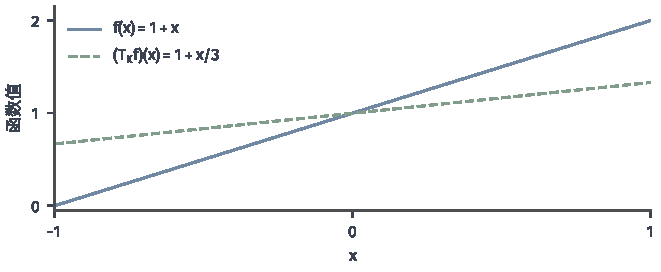
\includegraphics[width=112mm]{figures/01-mathematical-preliminaries-upper/02-linear-algebra-and-geometry/matplotlib/comprehension-additions/functional-integral-operator-action.pdf}
  \caption{$K(x,z)=1+xz$、$\mathrm d\mu=\mathrm dz/2$下，$f(x)=1+x$（实线）与其积分像$(T_Kf)(x)=1+x/3$（虚线）。积分把斜率压到原来的$1/3$，常数分量不动：正特征值$1$与$1/3$分别作用在常数与线性方向上。}
  \label{fig:vol1-add-functional-integral-operator-action}
\end{figure}

在归一测度下算谱。$T_K1=\int1\,\mathrm d\mu=1$，故$\psi_1=1$、$\mu_1=1$；$T_Kx=\int z\,\mathrm d\mu+x\int z^2\,\mathrm d\mu=x/3$，故$\psi_2=\sqrt3\,x$（归一：$\int 3x^2\,\mathrm d\mu=1$）、$\mu_2=1/3$。其余与$1,x$正交的方向属于零空间；两个正谱方向只覆盖仿射子空间，不能说整个$L^2[-1,1]$只有两个方向。

对$f=a+bx$，谱系数$b_1=\langle f,\psi_1\rangle=a$、$b_2=\langle f,\psi_2\rangle=b/\sqrt3$，故
\begin{equation}
\label{eq:functional-affine-two-norms}
\|f\|_{L^2(\mu)}^2=a^2+\frac{b^2}{3},\qquad
\|f\|_{H_K}^2=\frac{b_1^2}{\mu_1}+\frac{b_2^2}{\mu_2}=a^2+b^2.
\end{equation}
取$f=1+x$时两者分别为$4/3$和$2$；截到常数方向的尾误差平方分别为$1/3$和$1$，可与上面两种尾误差逐项核对。该谱例沿用前面同一仿射核空间，但额外加入测度后才取得积分特征值；改变测度会改变积分谱与$L^2$归一方向，不会自动改变原核通过再生关系定义的内积。

\subsection{积分方程的迭代求解}
\label{subsec:integral-equation-iteration}

前面给定函数计算积分输出；这里改为给定积分规则和外部项，寻找满足方程的未知函数。两项围绕同一名义方程，仅改变更新是否精确执行；表示截断与惩罚参数极限归入各自任务，不在这里混用。

\subsubsection{自映射与压缩条件}
\label{subsubsec:self-map-contraction}

固定$g\in C([a,b])$、紧矩形$[a,b]\times[a,b]$上连续的实核$K$与参数$\lambda$，要求未知函数$f\in C([a,b])$满足第二类Fredholm积分方程
\begin{equation}
\label{eq:functional-fredholm-equation}
f(x)=g(x)+\lambda\int_a^b K(x,t)f(t)\,\mathrm dt.
\end{equation}
把右端记为$Tf$：积分部分是线性算子，加入固定$g$后$T$是仿射映射。目标是求解该方程，即找$T$的不动点，而不只是生成一条没有解释对象的函数序列。

先核对$T$确实把$C([a,b])$映回自身。$K$在紧矩形上联合连续，故有界且一致连续。对固定连续$f$，
\[
|Tf(x)-Tf(z)|\le|g(x)-g(z)|+|\lambda|\|f\|_\infty\int_a^b|K(x,t)-K(z,t)|\,\mathrm dt;
\]
右端两项随$|x-z|\to0$一致趋于零，故$Tf$连续。$C([a,b])$在一致范数$\|\cdot\|_\infty$下完备。

接下来需要一个不动点存在定理，即\term{压缩映射}定理。它在本章本地完整建立，而不是引用别处结论。

\begin{theorem}[压缩映射定理（Banach不动点）]
\label{thm:banach-fixed-point}
设$(X,d)$为完备度量空间，$T:X\to X$满足压缩条件：存在$0\le q<1$使
\[
d(Tu,Tv)\le q\,d(u,v)\qquad(\forall u,v\in X).
\]
则$T$存在唯一不动点$x_*$。任取初值$x_0$，迭代$x_{k+1}=Tx_k$收敛于$x_*$，且
\begin{equation}
\label{eq:functional-iteration-apriori}
d(x_k,x_*)\le\frac{q^k}{1-q}\,d(x_1,x_0),
\end{equation}
\begin{equation}
\label{eq:functional-iteration-aposteriori}
d(x_k,x_*)\le\frac{q}{1-q}\,d(x_k,x_{k-1})\qquad(k\ge1).
\end{equation}
\end{theorem}

\begin{proof}
压缩映射连续：$d(Tx,Ty)\le q\,d(x,y)\to0$。逐步递推给出相邻步误差
\[
d(x_{n+1},x_n)\le q\,d(x_n,x_{n-1})\le\cdots\le q^n d(x_1,x_0).
\]
对$m>n$用三角不等式与几何级数，
\[
d(x_m,x_n)\le\sum_{j=n}^{m-1}d(x_{j+1},x_j)
\le d(x_1,x_0)\sum_{j=n}^{m-1}q^j
\le\frac{q^n}{1-q}d(x_1,x_0)\to0.
\]
$(x_n)$是Cauchy列；$X$完备，$x_n\to x_*$。由$T$连续，$Tx_*=\lim Tx_n=\lim x_{n+1}=x_*$，不动点存在。

唯一性：若$x_*,y_*$均为不动点，$d(x_*,y_*)=d(Tx_*,Ty_*)\le q\,d(x_*,y_*)$，$q<1$迫使$d(x_*,y_*)=0$。

先验界：在上面的逐步递推中令$m\to\infty$，
\[
d(x_*,x_n)\le\frac{q^n}{1-q}d(x_1,x_0).
\]
后验界：$d(x_n,x_*)\le q\,d(x_{n-1},x_*)$，故
\[
d(x_{n-1},x_*)\le d(x_{n-1},x_n)+d(x_n,x_*)\le d(x_{n-1},x_n)+q\,d(x_{n-1},x_*),
\]
整理得$(1-q)d(x_{n-1},x_*)\le d(x_{n-1},x_n)$，即$d(x_n,x_*)\le\frac{q}{1-q}d(x_n,x_{n-1})$。
\end{proof}

回到积分方程。对任意$f,h\in C([a,b])$，先在积分内作差再取绝对值，
\[
|Tf(x)-Th(x)|\le|\lambda|\|f-h\|_\infty\int_a^b|K(x,t)|\,\mathrm dt,
\]
故
\[
\|Tf-Th\|_\infty\le q\|f-h\|_\infty,\qquad
q=|\lambda|\sup_{x\in[a,b]}\int_a^b|K(x,t)|\,\mathrm dt.
\]
$q$必须对所有输入函数统一且满足$q<1$，不能用某次更新恰好变小代替严格压缩条件。自映射、完备与统一$q<1$齐备，定理\ref{thm:banach-fixed-point}给出唯一不动点$f_*$；由$T$的定义式，$f_*$正是方程\eqref{eq:functional-fredholm-equation}的解。

\subsubsection{精确更新与执行误差}
\label{subsubsec:exact-inexact-updates}

\paragraph{精确迭代的收敛与停止误差}

固定同一$g,K,\lambda$及初值$f^{(0)}\in C([a,b])$，令$f^{(k+1)}=Tf^{(k)}$。由刚核对的条件，精确迭代在一致范数中趋向唯一解$f_*$；方程与名义更新映射不变，变化的只是迭代中的近似函数。

先验界\eqref{eq:functional-iteration-apriori}说明误差只需初始更新差$\|f^{(1)}-f^{(0)}\|_\infty$与预先取得的$q$估计；后验界\eqref{eq:functional-iteration-aposteriori}说明已算出的相邻差$\|f^{(k)}-f^{(k-1)}\|_\infty$可直接用于停止判断。$q$接近一时必须保留$1/(1-q)$的放大因子：相邻变化小不直接等于误差同样小。$q\ge1$只使压缩论证失去保证，并不推出积分方程无解或多解；若要继续，须用别的条件另证。

\paragraph{同一方程下的扰动迭代}

保持同一名义$T$，实际更新未必精确执行：设
\[
\|f^{(k+1)}-Tf^{(k)}\|_\infty\le\eta_k,
\]
记$e_k=\|f^{(k)}-f_*\|_\infty$。先以三角不等式分离执行误差与名义输出差，再用压缩条件，
\begin{equation}
\label{eq:functional-perturbed-iteration}
e_{k+1}
\le\|f^{(k+1)}-Tf^{(k)}\|_\infty+\|Tf^{(k)}-Tf_*\|_\infty
\le\eta_k+q\,e_k.
\end{equation}
$\eta_k$可表示数值积分与更新造成的、对更新后整个函数的一致偏差，但不能把未经比较的模型差异也塞入其中。

反复展开递推：
\begin{equation}
\label{eq:functional-perturbed-unrolling}
e_k\le q^k e_0+\sum_{j=0}^{k-1}q^{\,k-1-j}\eta_j.
\end{equation}
初值影响随迭代按$q^k$衰减；历次执行误差按剩余更新次数加权。若$\eta_j\le\eta$一致，几何级数给出
\[
\limsup_{k\to\infty}e_k\le\frac{\eta}{1-q}.
\]
这是持续执行误差造成的误差地板上界，不保证每条轨迹收敛，更不保证误差恰好达到该边界。

若$\eta_j\to0$，把误差和分为有限早期项与尾部：对固定$J$，$j\le J$的有限项因几何权重$q^{k-1-j}\to0$而消失；$j>J$的尾部由$\sup_{j>J}\eta_j$乘$1/(1-q)$控制。取$J$足够大使尾部界任意小，再令$k\to\infty$，即得$e_k\to0$。更一般的可求和条件可作为同一分解的充分情形。比较持续与衰减执行误差时始终固定方程、初值和名义$q$，改变的仅是执行精度。若实际近似函数不在所定连续空间中，或自映射、完备、严格压缩任一项缺失，都须重建适用框架；这些限制与$q\ge1$的边界共同保留。
\section{泛函变分与函数拟合}
\label{sec:variational-functional-fitting}

前面各节把函数作为已知对象，研究怎样合法地读取它、用它构造算子或把它分解成正交方向。本节把函数改为未知量：候选函数本身是优化变量，我们要在给定候选空间、给定观测数据和给定偏差计量下，判断最优函数是否存在、是什么形状、对数据扰动有多敏感。三个任务分别规定不同的观测类型：有限个线性读数、整个定义域上的目标函数值，以及希望逼近的梯度向量场。变分提供这些任务共用的扰动语言——用$f+th$代替整条函数并考察目标的一阶变化；观测类型不同，可行扰动和残差计价就不同。不同任务也可以组合，例如同时拟合函数值和梯度场，但组合时必须写出共同候选空间、完整目标和各项权重，不能仅凭惩罚名称判断任务。

本节把每个拟合任务的识别、计算、数据扰动和参数极限放在相应问题内分别回答。一次最优化是否达到下确界、最优函数是否唯一、系数是否唯一、迭代算法是否收敛，是四个不同的判断；改变数据、改变惩罚参数与增加计算次数也不是同一个极限，后面凡涉及“收敛”或“稳定”都指明固定了什么、改变了什么。

\subsection{泛函微分与最优条件}
\label{subsec:functional-differential-optimality}

先在给定函数空间中说明怎样改变整条函数并计量目标的一阶响应，随后把同一扰动语言用于抽象目标和积分目标。微分只给出一阶变化的线性读数；最优条件还要考虑哪些扰动在当前候选下可行；这些条件本身是驻点刻画，不保证最小值达到，也不替代存在性证明。

\subsubsection{方向导数、Fréchet微分与梯度}
\label{subsubsec:frechet-gradient}

\paragraph{从函数扰动到有界线性微分}

固定实Hilbert空间$H$，其内积与范数分别记作$\langle\cdot,\cdot\rangle_H$与$\|\cdot\|_H$，令$J:H\to\mathbb R$在$f$的某个开邻域内取有限实值。先把“对函数求导”与熟悉的“对输入位置求导”分开：$f'(x)$描述函数值随位置$x$的变化，这里固定整条函数$f$不动，让它作为一个整体沿某个方向$h\in H$移动，考察目标值的响应。取实数$t$，用$f+th$改变整条函数，在固定$h$时定义
\[
  \mathrm d_hJ(f)
  =\lim_{t\to0}\frac{J(f+th)-J(f)}{t};
\]
这个极限称为$J$在$f$沿方向$h$的\term{方向导数}。它回答“目标对函数沿$h$的微小整体变化有多敏感”，与$f'(x)$是两类不同的微分。

逐个方向固定$h$取极限，只能核对“每条射线方向上目标都有线性响应”，不能控制许多方向同时变化时小扰动的合力。这正如有限维中各方向偏导数存在不保证可微：方向导数沿离散方向都存在，仍可能在斜向上突然失效。为此要求一个统一的一阶近似：存在一个有界线性泛函$DJ(f):H\to\mathbb R$，使$h$足够小时
\begin{equation}
  J(f+h)=J(f)+DJ(f)[h]+r_f(h),\qquad
  \frac{|r_f(h)|}{\|h\|_H}\to0\quad(\|h\|_H\to0).
  \label{eq:functional-frechet-differential}
\end{equation}
\begin{definition}[方向导数与Fréchet微分]\label{def:functional-frechet}
设$H$为实Hilbert空间，$J$在$f$附近有限。若对一切$h\in H$方向导数存在，则称$J$在$f$处有方向导数；若还存在有界线性泛函$DJ(f)$使式~\eqref{eq:functional-frechet-differential}的余项满足$|r_f(h)|/\|h\|_H\to0$，则称$J$在$f$处Fréchet微分可微，$DJ(f)$为其Fréchet微分（亦称\term{Fréchet导数}）。
\end{definition}
余项条件是对所有趋零扰动同时提出的：它要求余项比任意一阶位移都更小，而不是逐方向分别趋零。因此，每个方向导数存在并不直接推出Fréchet可微；要拿到统一估计，还须另行证明。

Fréchet微分$DJ(f)$是有界线性泛函，输出只是一个数。第~\ref{subsubsec:riesz-representation}节已经证明，实Hilbert空间中每个有界线性泛函$L$都唯一对应一个方向$h_L$使$L(h)=\langle h,h_L\rangle_H$。把这个结论用于$DJ(f)$，存在唯一的$\nabla_HJ(f)\in H$使
\[
  DJ(f)[h]=\langle\nabla_HJ(f),h\rangle_H,
\]
称$\nabla_HJ(f)$为$J$在$f$处关于内积$\langle\cdot,\cdot\rangle_H$的\term{梯度}。微分与梯度由此分开：微分对扰动输出标量读数，梯度是在当前内积下表示这个读数的那个空间方向；更换内积会更换代表方向，却不更换微分本身。不能把这两个对象当成同一个公式名称，也不能脱离内积谈“梯度就是微分”。

\paragraph{改变内积时的梯度}

下面用一个可逐项复算的例子核对微分、余项与梯度的关系，并直接观察“微分不变、梯度随内积改变”。取仿射函数空间
\[
  H=\{f:x\mapsto a+bx:a,b\in\mathbb R\},
\]
它是维数为二的实Hilbert空间。在这个空间上定义目标
\[
  J(f)=\frac{a^2+b^2}{2}.
\]
对任意扰动$h(x)=u+vx$，展开
\[
\begin{aligned}
  J(f+th)
  &=\frac{(a+tu)^2+(b+tv)^2}{2}\\
  &=J(f)+t(au+bv)+\frac{t^2(u^2+v^2)}{2}.
\end{aligned}
\]
因此沿$h$的方向导数为$au+bv$，且余项$r_f(th)=t^2(u^2+v^2)/2$满足
\[
  \frac{|r_f(th)|}{\|th\|_H}\to0
\]
只要所选范数等价于系数欧氏范数。线性部分$DJ(f)[h]=au+bv$与所选内积无关；它是否Fréchet可微，由余项比一阶位移更小这一条件核对，上式同时给出了线性部分和余项的量级。

第一种内积取系数内积
\[
  \langle a+bx,u+vx\rangle_1=au+bv.
\]
此时直接看出$\nabla_{H,1}J(f)=a+bx$，因为$\langle a+bx,u+vx\rangle_1=au+bv=DJ(f)[h]$。

第二种内积改用$[-1,1]$上$\mathrm d\mu=\mathrm dx/2$的$L^2$内积。逐项积分：
\[
\begin{aligned}
  \langle a+bx,u+vx\rangle_2
  &=\int_{-1}^1(a+bx)(u+vx)\,\frac{\mathrm dx}{2}\\
  &=au\int\frac{\mathrm dx}{2}
  +(av+bu)\int x\,\frac{\mathrm dx}{2}
  +bv\int x^2\,\frac{\mathrm dx}{2}\\
  &=au+\frac{bv}{3},
\end{aligned}
\]
其中奇函数项在对称区间上积分为零，$\int x^2\,\mathrm dx/2=1/3$。要求梯度$g(x)=\alpha+\beta x$满足
\[
  \langle g,u+vx\rangle_2=\alpha u+\frac{\beta v}{3}=au+bv
  \]
对所有$u,v$成立，解得$\alpha=a$、$\beta=3b$，即
\[
  \nabla_{H,2}J(f)=a+3bx.
\]
两种内积在这个有限维空间里拓扑等价，目标$J$和微分$DJ(f)[h]=au+bv$都没有改变，改变的只是表示该读数的空间方向。这个例子为后面区分“目标变化”与“优化几何变化”提供可复算的依据：同一个$J$，在系数内积下沿$(1,0)$走一步最陡，在$L^2$内积下最陡方向的系数变成$(1,3)$。

\subsubsection{可行扰动、最优条件与梯度流}
\label{subsubsec:feasible-optimality-flow}

\paragraph{凸约束下的一阶条件}

无约束时可以沿$+h$和$-h$两个方向试走；候选集$C$为凸集但不含内点时，边界上的候选可能只允许向一侧移动，因此一阶条件必须按“哪些扰动可行”来表述。

给定非空\term{凸集}$C\subset H$：对任意$f_1,f_2\in C$，线段$(1-t)f_1+tf_2$（$0\le t\le1$）也在$C$中。设$f_*\in C$是$J$在$C$上的最小点，对任意$g\in C$，凸性保证
\[
  f_*+t(g-f_*)\in C,\qquad 0\le t\le1.
\]
因为$f_*$最小，对$t>0$有$J(f_*+t(g-f_*))\ge J(f_*)$。若$J$在$f_*$Fréchet可微，令$t\downarrow0$，由方向导数的定义得到
\begin{equation}
  DJ(f_*)[g-f_*]\ge0,\qquad\forall g\in C.
  \label{eq:functional-convex-optimality}
\end{equation}
这就是最小点必须满足的一阶条件。注意这里$g-f_*$只能沿从$f_*$指向$C$内部的方向取；在边界附近不能任取正负扰动，否则会跑出候选集。

在这个必要条件之上加凸性，可以取得充分性。

\begin{theorem}[凸候选集上的一阶最优条件]\label{thm:functional-convex-optimality}
设$C\subset H$非空凸，$J$在$C$上凸，且在$f_*\in C$的开邻域内Fréchet可微。则$f_*$是$J$在$C$上的最小点，当且仅当
\[
  DJ(f_*)[g-f_*]\ge0,\qquad\forall g\in C.
\]
\end{theorem}

\begin{proof}
必要性已在上面给出：最小点向任意可行方向的一阶响应不能为负。

充分性使用\term{凸函数}的一阶下界：对凸且Fréchet可微的$J$，有
\[
  J(g)\ge J(f_*)+DJ(f_*)[g-f_*],\qquad\forall g\in C.
\]
（这是一维凸函数切线不等式$\varphi(t)\ge\varphi(0)+\varphi'(0)t$在Hilbert空间中的版本，由$J(f_*+t(g-f_*))$关于$t$的凸性对$t\ge0$展开取得。）再由条件$DJ(f_*)[g-f_*]\ge0$，右端不小于$J(f_*)$，即$J(g)\ge J(f_*)$对所有$g\in C$成立。
\end{proof}

定理先说明“最小点必有此不等式”（必要性），再增加凸性取得“满足此不等式即全局最优”（充分性）。存在性、严格凸时的至多唯一性、以及最小者实际是否达到，仍是另外的问题：本定理不证明下确界被取得，也不把驻点条件推广到非凸目标。

\paragraph{梯度流的能量变化及边界}

在无约束$H$上，沿梯度方向下降是最熟悉的一阶迭代语言。设曲线$f(t)$对$t$可微，且$J$可用链式法则求复合导，定义梯度流
\[
  \dot f(t)=-\nabla_HJ(f(t)).
\]
把链式法则写成一阶响应的形式：
\[
  \frac{\mathrm d}{\mathrm dt}J(f(t))
  =DJ(f(t))[\dot f(t)].
\]
代入$\dot f=-\nabla_HJ(f)$，由Riesz表示$DJ(f)[\nabla_HJ(f)]=\langle\nabla_HJ(f),\nabla_HJ(f)\rangle_H=\|\nabla_HJ(f)\|_H^2$，得到能量恒等式
\[
  \frac{\mathrm d}{\mathrm dt}J(f(t))
  =-\|\nabla_HJ(f(t))\|_H^2\le0.
\]
这说明了为什么该方向使目标下降：每一步的一阶响应恰好是梯度范数的平方。但这个恒等式只是在一条已经存在的解曲线上核算能量变化，并不是解曲线存在的证明；仅有下降还不足以推出全局存在性、轨迹收敛到某个函数、或收敛到全局最小者。此外，有约束候选$C$上不能直接套用这个无约束方程，须另给投影或可行保持机制；目标不可微时，须另用\term{次梯度}等适当条件。具体热演化方程的全局存在、收敛和长时间行为由后续微分方程章建立，本节只保留目标、梯度和能量变化的共同接口。

\subsubsection{积分泛函的内部条件与边界条件}
\label{subsubsec:integral-functional-variation}

\paragraph{局部密度的一阶变化}

前面的扰动语言不依赖$J$的具体形式。下面把它用于一类最重要的目标——逐点积分密度。设$\Omega\subset\mathbb R^d$为有界光滑域，$u:\Omega\to\mathbb R^r$可以有多个分量，$F:\Omega\times\mathbb R^r\times\mathbb R^{r\times d}\to\mathbb R$可以耦合各分量，考虑
\[
  J(u)=\int_\Omega F(x,u,\nabla u)\,\mathrm dx.
\]
先在$u,h,F$都足够光滑、且允许把导数移入积分的支配条件下计算一阶变化。对每个分量$u_a$及其梯度$\nabla u_a$作一阶展开：
\[
  F(x,u+h,\nabla u+\nabla h)
  =F(x,u,\nabla u)
  +\sum_a\left(F_{u_a}h_a+F_{\nabla u_a}\cdot\nabla h_a\right)+o(\|h\|_{C^1}),
\]
其中$F_{u_a}$是$F$对$u_a$的偏导，$F_{\nabla u_a}$是对该分量梯度的偏导向量。除以$t$并令$t\to0$（余项由支配条件一致地趋于零），得到
\begin{equation}
  \delta J(u)[h]
  =\int_\Omega\sum_a
  \left(F_{u_a}h_a+F_{\nabla u_a}\cdot\nabla h_a\right)\mathrm dx.
  \label{eq:functional-general-euler-lagrange-variation}
\end{equation}
光滑性和可移项条件不足时，不能把这个经典计算自动推广到任意Sobolev目标；那时应保留积分形式本身，而不把它点态化。

一阶变化由两部分组成。对梯度项作分部积分（高维用散度定理）：对每个分量$a$，把向量场$F_{\nabla u_a}h_a$的散度展开为$\operatorname{div}(F_{\nabla u_a}h_a)=(\operatorname{div}F_{\nabla u_a})h_a+F_{\nabla u_a}\cdot\nabla h_a$，
\[
  \int_\Omega F_{\nabla u_a}\cdot\nabla h_a\,\mathrm dx
  =\int_{\partial\Omega}(F_{\nabla u_a}\cdot n)h_a\,\mathrm dS
  -\int_\Omega \operatorname{div}(F_{\nabla u_a})h_a\,\mathrm dx,
\]
其中$n$是$\partial\Omega$的单位外法向量；左边是被积分进去的梯度项，导数$\partial_i$全部落在$h_a$上。代入式~\eqref{eq:functional-general-euler-lagrange-variation}，一阶变化被分成内部项与边界项两部分：
\[
  \delta J(u)[h]
  =\int_\Omega\sum_a
  \left(F_{u_a}-\operatorname{div}F_{\nabla u_a}\right)h_a\,\mathrm dx
  +\int_{\partial\Omega}\sum_a
  \left(F_{\nabla u_a}\cdot n\right)h_a\,\mathrm dS.
\]
内部项只含扰动$h_a$本身，边界项只含$h_a$在边界上的迹。这一步说清了一阶变化的两个不同来源；后面判断驻点条件时，正是可行扰动的边界值决定两项各自由谁负责。

\paragraph{可行边界如何决定条件}

驻点要求$\delta J(u)[h]=0$对所有合法扰动$h$成立，而“合法”由候选集合规定。

若候选固定迹：$u$与$u+h$有相同的边界值$g=\operatorname{Tr}u$，则允许扰动的边界迹为零，边界项恒为零。此时内部项必须对所有$h$成立，由变分法基本引理（测试函数任意时积分恒为零迫使被积函数为零）取得内部条件
\[
  F_{u_a}-\operatorname{div}F_{\nabla u_a}=0,\qquad a=1,\ldots,r,
\]
即各分量的Euler--Lagrange方程。

若某个分量在边界上自由，该分量扰动的边界迹可以独立变化，则边界项独立地要求
\[
  F_{\nabla u_a}\cdot n=0\quad\text{在$\partial\Omega$上},
\]
这就是该分量的自然边界条件（自然通量为零）。混合边界要逐部分核对：固定迹处不重复要求自然通量，自由迹处才要求通量为零；把固定迹处也写上零通量是错误的，因为那里根本没有边界项负责。

当经典二阶导数或点态通量尚无意义时（候选只是Sobolev函数），应保留原来对所有合法测试扰动成立的一阶积分式~\eqref{eq:functional-general-euler-lagrange-variation}，而不是先点态化再谈散度。凸密度$F$在相应可积范围内使积分目标凸，配合仿射可行集（如固定迹的$G+H_0^1$），可以把上面的驻点条件用于充分性判断；非凸情形的唯一性与达到性仍需另证。下文梯度场拟合把各自密度代入这套运算，不再重复建立多分量框架。

\subsection{有限线性观测下的函数拟合}
\label{subsubsec:finite-observation-fitting}

现在进入具体的拟合任务。给定$n$个有界线性读取$L_i:H\to\mathbb R$及目标数值$y_i$，数据只约束$n$个读数。先检查这组数据是否相容、是否唯一确定候选；再说明单调不减的范数惩罚怎样消去数据看不见的方向；最后把函数目标化为有限参数问题。点值拟合只有在相应空间中点读数合法且有界时才属于这个范围——第~\ref{subsubsec:point-evaluation}节已经说明，在$L^2$等空间里点读数甚至不被范数控制。

\subsubsection{读数的相容性与可识别性}
\label{subsubsec:identifiability}

\paragraph{候选范围与不可见方向}

固定候选$C\subseteq H$和读数映射
\[
  L:f\mapsto(L_1f,\ldots,L_nf)\in\mathbb R^n.
\]
给定观测$y=(y_1,\ldots,y_n)^{\top}$，与之相容的候选集合为
\[
  \{f\in C:Lf=y\}.
\]
这个集合的非空性回答相容性：数据能否被某个候选达到。它恰有一个元素，回答的是“在这一组特定数据下候选是否唯一确定”。而$L$在整个$C$上的单射性要求更强：对所有可能的$y$，相容集合都至多有一个元素。这一单射性的准确表述是：任意两个相容候选之差不能落在零读数空间里，即$(C-C)\cap\ker L=\{0\}$；当$C$本身是线性子空间时，它才简化为$\ker L\cap C=\{0\}$。三者量词不同：相容性是“存在$f$使$Lf=y$”，数据下唯一是“恰有一个$f$”，映射单射是“一切$y$都至多一个$f$”；不能把针对一个$y$的判断替换成整个映射的单射性。

即使候选是有限维线性空间，也会因读取矩阵秩亏而不可识别。取$C=\{f(x)=a+bx\}$只读$f(0)$，数据$f(0)=a_0$确定系数$a$却不限制$b$，整条直线斜率任意。再看无限维例子：取两个函数
\[
  f(x)=0,\qquad g(x)=x(x^2-1),
\]
它们在$-1,0,1$三个位置都给出零读数，却是不同的函数；一般地，任何“在所有观测点为零”的多项式加到$g$上都不改变读数。图~\ref{fig:vol1-add-functional-unseen-observation-direction}画出了这种不可见方向。

\begin{figure}[!htb]
  \centering
  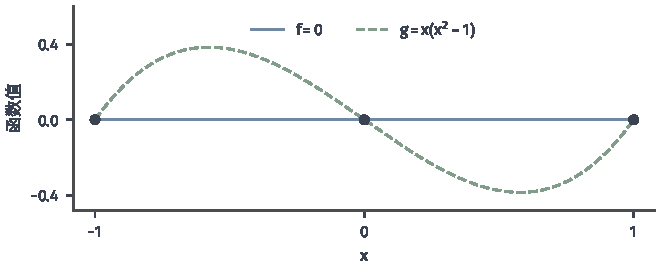
\includegraphics[width=112mm]{figures/01-mathematical-preliminaries-upper/02-linear-algebra-and-geometry/matplotlib/comprehension-additions/functional-unseen-observation-direction.pdf}
  \caption{有限点值留下不可见方向。定义域为$[-1,1]$，黑点为$x=-1,0,1$处的零读数。蓝线$f=0$与绿虚线$g(x)=x(x^2-1)$在三个位置完全一致，在其余位置可以不同。此处候选范围包含这些多项式；若另行限制次数或范数，仍须重新判断读取是否单射及候选是否可行。}
  \label{fig:vol1-add-functional-unseen-observation-direction}
\end{figure}

增加多项式次数、范数球或其他约束后，应在新的实际候选中重新检查哪些差函数仍可行：$g$不在新候选里，不可见方向就消失了。惩罚的作用是从同读数的多个函数中选定一个，它没有让原始数据获得额外识别能力——数据本身仍然看不见惩罚选定的方向。下一项用正交分解解释这种选择为什么能把搜索范围有限化。

\subsubsection{范数惩罚下的表示定理}
\label{subsubsec:representer-theorem}

\paragraph{用正交分解消去数据看不见的余项}

在实Hilbert空间$H$中取$n$个有界线性读取$L_i$。由第~\ref{subsubsec:riesz-representation}节的Riesz表示定理，每个$L_i$对应唯一方向$h_i\in H$使
\[
  L_i(f)=\langle f,h_i\rangle_H,\qquad i=1,\ldots,n.
\]
令
\[
  M=\operatorname{span}\{h_1,\ldots,h_n\}.
\]
$M$是有限维子空间；有限维子空间在Hilbert空间中闭（有限维空间上所有范数等价，柯西列必在该维数内收敛）。由第~\ref{subsubsec:orthogonal-projection}节的闭子空间投影结论，每个$f\in H$都有唯一正交分解
\[
  f=P_Mf+r,\qquad r\perp M,
\]
且$\|P_Mf\|_H\le\|f\|_H$。由$r\perp h_i$直接得到
\[
  L_i(r)=\langle r,h_i\rangle_H=0,\qquad i=1,\ldots,n,
\]
即余项$r$对全部读数不可见。这一步说明为什么去掉余项不改变数据项：不是“余项很小”，而是读数在$r$上恒为零。

现在考虑目标
\[
  J(f)=\Phi(Lf)+\Omega(\|f\|_H),
\]
其中$\Phi:\mathbb R^n\to\mathbb R$是读数代价，$\Omega:[0,\infty)\to\mathbb R$单调不减。因为$L_i(r)=0$，有$L(P_Mf)=Lf$，故$\Phi$两项相同；由$\|P_Mf\|_H\le\|f\|_H$及$\Omega$单调不减，得
\[
  J(P_Mf)=\Phi(Lf)+\Omega(\|P_Mf\|_H)
  \le\Phi(Lf)+\Omega(\|f\|_H)=J(f).
\]
于是在$M$中搜索与在全空间$H$中搜索取得相同下确界：任何$f$都被它的投影$P_Mf$（属于$M$）以不更差的目标取代。

\begin{theorem}[有限读取下的表示定理]\label{thm:functional-representer}
设$H$为实Hilbert空间，$L_1,\ldots,L_n$为有界线性读取，$h_i$为其Riesz方向，$M=\operatorname{span}\{h_i\}$。设
\[
  J(f)=\Phi(Lf)+\Omega(\|f\|_H),
\]
其中$\Phi$任意，$\Omega:[0,\infty)\to\mathbb R$单调不减。则：
\begin{enumerate}
  \item $\inf_{f\in H}J(f)=\inf_{f\in M}J(f)$；若$J$在$H$上达到最小值，则至少存在一个最小点属于$M$。
  \item 若$\Omega$还严格递增，且$J$达到最小值，则每个最小点都属于$M$。
  \item 若另有限制$C\subseteq H$代替全空间，上述结论在$P_M(C)\subseteq C$时成立；否则删除余项可能破坏可行性。
\end{enumerate}
\end{theorem}

\begin{proof}
对任意$f\in H$，上面已证$J(P_Mf)\le J(f)$且$P_Mf\in M$，故$\inf_{f\in M}J\ge\inf_{f\in H}J$，反向不等式由$M\subset H$直接得到，两端相等。若$f_*$是$H$上的最小点，则$J(P_Mf_*)\le J(f_*)$；又因$f_*$最小，$J(P_Mf_*)\ge J(f_*)$，故$P_Mf_*$也是最小点且属于$M$，本定理第一点成立。

若$\Omega$严格递增，且$f_*$的余项$r=f_*-P_Mf_*\ne0$，则$\|P_Mf_*\|<\|f_*\|$，由严格递增得$\Omega(\|P_Mf_*\|)<\Omega(\|f_*\|)$，从而$J(P_Mf_*)<J(f_*)$，与$f_*$最小矛盾；故$r=0$，即$f_*\in M$，本定理第二点成立。

有$C$限制时，$P_Mf$必须仍落在$C$中，上述投影取代才合法；第~3点的投影保持条件由此而来。
\end{proof}

注意定理没有说：下确界一定达到、最小函数唯一、或系数唯一。表示形式只是把搜索空间降到$M$，存在性与唯一性仍要由具体$\Phi,\Omega$另行判断。

\paragraph{惩罚含义与附加约束}

同为范数惩罚，$\Omega$所控制的对象由空间和范数的定义决定：$L^2$范数只累计函数值整体大小，整数阶Sobolev范数还累计规定阶弱导的整体大小，RKHS范数通过核截面同时控制点值稳定性和两点差，Lipschitz约束则直接限制函数随输入的变化幅度。不能笼统地把所有范数惩罚称为“让函数每点、每阶导数都同样平滑”。

点读取对应$h_i=K_{x_i}$（再生核截面，见第~\ref{subsubsec:point-evaluation}节），一般线性读取仍用各自的Riesz方向$h_i$；两者共用上面的证明，只是$h_i$的具体来源不同。附加约束方面，核范数球和仅依赖这组读数的约束可以逐项检查投影保持性$P_M(C)\subseteq C$，任意约束不可默认满足。完成这些条件后，才进入实际的有限参数目标。图~\ref{fig:representer-finite-readings-to-solver}把整个流程串起来。

\begin{figure*}[htbp]
  \centering
  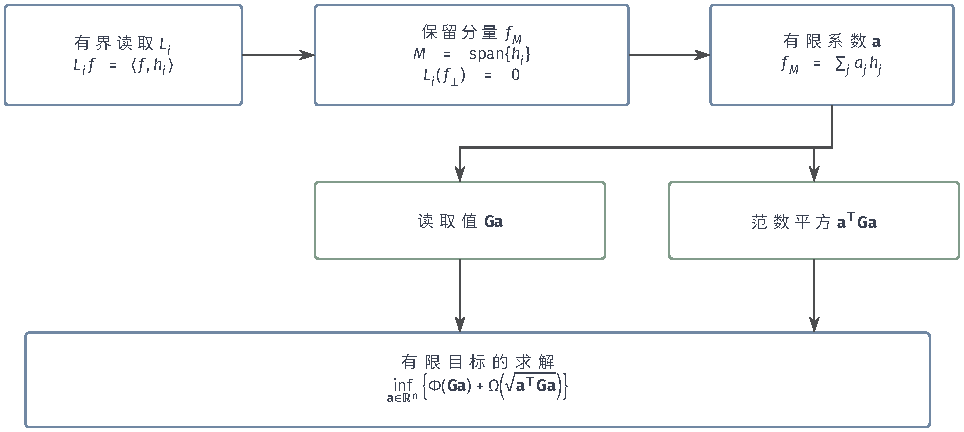
\includegraphics[width=163.258mm]{figures/01-mathematical-preliminaries-upper/02-linear-algebra-and-geometry/tikz/representer-finite-readings-to-solver/source.pdf}
  \caption{有限读取下的表示与求解。有界线性泛函$L_i$在Hilbert空间中有Riesz表示元$h_i$。所有读取只依赖$M=\operatorname{span}\{h_i\}$中的分量$f_M$，单调不减的范数惩罚允许删去$f_\perp$而不增大目标。写$f_M=\sum_j a_jh_j$后，读数与范数平方分别为$\bm G\bm a$与$\bm a^{\top}\bm G\bm a$。将这两个有限表达式代入目标后即可求解系数；最优解存在与系数唯一仍需另行判断。}
  \label{fig:representer-finite-readings-to-solver}
\end{figure*}

\subsubsection{Gram矩阵与平方拟合}
\label{subsubsec:gram-least-squares}

\paragraph{从函数目标到参数目标}

把$M$中的函数写成$f=\sum_{j=1}^n a_jh_j$，定义\term{Gram矩阵}
\[
  G_{ij}=\langle h_j,h_i\rangle_H=L_i(h_j),\qquad i,j=1,\ldots,n.
\]
逐项计算读数与范数：
\[
  (Lf)_i=L_i(f)=\sum_j a_jL_i(h_j)=\sum_jG_{ij}a_j,
\]
即$Lf=Ga$；以及
\begin{equation}
  \|f\|_H^2
  =\left\langle\sum_ja_jh_j,\sum_k a_kh_k\right\rangle_H
  =\sum_{i,j}a_iG_{ij}a_j=a^{\top}Ga.
  \label{eq:functional-finite-gram-objective}
\end{equation}
于是表示定理把目标化为有限变量$a\in\mathbb R^n$的问题：
\[
  \inf_{a\in\mathbb R^n}\left\{\Phi(Ga)+\Omega\!\left(\sqrt{a^{\top}Ga}\right)\right\}.
\]
只有读取恰好是点值$L_i(f)=f(x_i)$时，$G_{ij}=\langle K_{x_j},K_{x_i}\rangle_H=K(x_i,x_j)$才把$G$写成核矩阵；一般线性读取的Gram矩阵仍由$G_{ij}=\langle h_j,h_i\rangle$定义，不能省去“一般读数到核矩阵”这层条件。

取平方数据代价与二次范数惩罚，固定$\lambda>0$，考虑
\begin{equation}
  J_y(f)=\frac1n\sum_{i=1}^n(L_if-y_i)^2+\lambda\|f\|_H^2.
  \label{eq:functional-regularized-least-squares}
\end{equation}
代入有限表示$J_y(a)=\frac1n\|Ga-y\|_2^2+\lambda a^{\top}Ga$，对$a_j$求导：
\[
  \frac{\partial J_y}{\partial a_j}
  =\frac{2}{n}\sum_iG_{ij}(Ga-y)_i+2\lambda(Ga)_j.
\]
写成矩阵形式，驻点要求
\[
  \frac2nG(Ga-y)+2\lambda Ga=0,
\]
即
\[
  G\bigl[(G+n\lambda I)a-y\bigr]=0.
\]
注意$G$半正定：$a^{\top}Ga=\|\sum_ja_jh_j\|_H^2\ge0$。因此$G+n\lambda I$严格正定（其特征值为$t+n\lambda\ge n\lambda>0$），可逆。选取使括号内直接为零的规范代表
\begin{equation}
  a=(G+n\lambda I)^{-1}y.
  \label{eq:functional-tikhonov-representer}
\end{equation}
这里特意保留前一个驻点方程$G[(G+n\lambda I)a-y]=0$：后一个可逆方程只是选定代表，它要求括号向量本身为零；而驻点条件只要求该向量落在$\ker G$中，并未要求每组冗余系数都满足可逆方程。

为什么这个规范代表给出唯一的最优函数？先用前面已证的表示定理（定理~\ref{thm:functional-representer}）把搜索压到有限维。本问题的数据项$\Phi(z)=\frac1n\|z-y\|^2$凸，惩罚$\Omega(t)=\lambda t^2$随$t$严格递增；该定理已给出$\inf_{f\in H}J_y(f)=\inf_{f\in M}J_y(f)$，并且任何在$M$内达到下确界的点自动是$H$上的全局最小点。于是只需在$M$上证明最小值达到且唯一。

在$M$内写$f=\sum_ja_jh_j$，目标是系数$a\in\mathbb R^n$的二次函数$J_y(a)=\frac1n\|Ga-y\|^2+\lambda a^{\top}Ga$。把系数空间拆成$\ker G$与它的正交补：若$\delta a\in\ker G$，则$G\delta a=0$且$\delta a^{\top}G\delta a=0$，沿这个方向数据项与惩罚项都不变——系数冗余不改变函数，目标真正依赖的是$a$在$(\ker G)^\perp$上的投影$a_\perp$。退化情形先单独处理：若$\operatorname{rank}G=0$，则$G=0$；由$a^{\top}Ga=\|\sum_ja_jh_j\|_H^2$对一切$a$为零，迫使每个$h_i=0$，从而所有读数$L_if=\langle f,h_i\rangle\equiv0$恒为零，$M=\{0\}$。此时式~\eqref{eq:functional-regularized-least-squares}化为$J_y(f)=\frac1n\|y\|_2^2+\lambda\|f\|_H^2$，它随$\|f\|_H$严格增大，唯一最小点为$f_*=0$，最小代价为$\frac1n\|y\|_2^2$。以下设$\operatorname{rank}G\ge1$。在这个补空间上$G$严格正定：它是有限维对称矩阵，正特征值$t_i>0$全部出现，故有正的最小特征值$t_{\min}>0$。于是
\[
  J_y(a)\ge \lambda a_\perp^{\top}G a_\perp\ge \lambda t_{\min}\|a_\perp\|^2,
\]
右端随$\|a_\perp\|$增大而无界，目标在$(\ker G)^\perp$上强制。任取$c$，次水平集$\{a_\perp:J_y(a)\le c\}$一方面被$\|a_\perp\|\le\sqrt{c/(\lambda t_{\min})}$有界，另一方面是连续函数$J_y$的闭集；有限维闭且有界的集合必紧，由连续函数在紧集上达到极值的Weierstrass定理，$J_y$在$(\ker G)^\perp$上达到最小；$\ker G$方向任取零点，即得$M$上达到下确界的系数代表。

最后唯一性：数据项$\frac1n\|Lf-y\|^2$关于$f$凸，惩罚项$\lambda\|f\|_H^2$在$\lambda>0$时严格凸，故$J_y$在$H$上严格凸；严格凸函数至多有一个最小点，而最小点已在$M$内达到，故最小函数唯一。

\begin{theorem}[平方读取加二次惩罚的解]\label{thm:functional-tikhonov-solution}
设$H$为实Hilbert空间，$\lambda>0$，并给定$n$个有界线性读取
\[
  L_i:H\to\mathbb R,\qquad i=1,\ldots,n.
\]
则式~\eqref{eq:functional-regularized-least-squares}存在唯一的全局最小函数$f_*\in H$，且$f_*\in M=\operatorname{span}\{h_i\}$。其规范系数代表由式~\eqref{eq:functional-tikhonov-representer}给出：该代表在所有$h_i$方向满足一阶条件
\[
  DJ_y(f_*)[h_i]=0,
\]
在$M^\perp$方向上读数不变且$f_*$与扰动正交，一阶条件同样成立。
\end{theorem}

这里用具体二次目标完成了存在与唯一的证明，不能把这个结论反推给表示定理中任意的$\Phi,\Omega$。

\paragraph{函数唯一与系数冗余}

$G$奇异与最优函数唯一可以同时成立。若$\delta a\in\ker G$，则
\[
  \left\|\sum_j\delta a_jh_j\right\|_H^2
  =\delta a^{\top}G\,\delta a=0,
\]
由范数正定性，这个线性组合就是零函数；所有读数也都不变。因此问题不在函数层——最优函数唯一——而在坐标层：同一个函数$f_*=\sum_ja_j^*h_j$可以写成许多组系数，差向量都沿$\ker G$。

有附加约束时，先重查投影保持性$P_M(C)\subseteq C$，再把约束写成实际参数可行集。有限化只给出一个有限变量问题，不指定任何具体迭代算法都能收敛；下一项把“改变数据”和“增加计算次数”两种误差分别比较。

\subsubsection{数据扰动与计算误差}
\label{subsubsec:finite-fit-stability-computation}

\paragraph{固定惩罚参数时的数据稳定性}

固定$L_i,G,\lambda$，把观测数据从$y$改为$y+\delta y$，其余一切不动。规范代表的差为
\[
  \delta a=(G+n\lambda I)^{-1}\delta y.
\]
函数误差不能直接用系数欧氏距离$\|\delta a\|_2$计量——同一函数可有多组系数；正确的函数范数差是
\[
  \|\delta f\|_H^2=\delta a^{\top}G\,\delta a.
\]

把$G$正交对角化：$G=Q\operatorname{diag}(t_1,\ldots,t_n)Q^{\top}$，$t_i\ge0$。记$\tilde y=Q^{\top}\delta y$，则
\[
  \|\delta f\|_H^2
  =\sum_i\frac{t_i}{(t_i+n\lambda)^2}\,\tilde y_i^{\,2}.
\]
对每个$t\ge0$，由$(t+n\lambda)^2\ge4tn\lambda$（展开$t^2+2tn\lambda+n^2\lambda^2\ge4tn\lambda$即$(t-n\lambda)^2\ge0$）得
\[
  \frac{t}{(t+n\lambda)^2}\le\frac{1}{4n\lambda}.
\]
零特征方向$t=0$的权重为零，不贡献函数误差。合并得到
\begin{equation}
  \|\delta f\|_H\le\frac{\|\delta y\|_2}{2\sqrt{n\lambda}}.
  \label{eq:functional-data-stability-bound}
\end{equation}
这个界说明当前归一化$1/n$与固定的$\lambda$如何进入稳定常数。它比较的是两个不同数据任务的精确最优函数之差：没有研究任何求解算法，也没有让$\lambda$趋零。若随数据改变读取位置$x_i$或更换核，$G$本身也改变，就不能继续使用同一个矩阵逆的差分式~\eqref{eq:functional-tikhonov-representer}。

\paragraph{固定任务中的参数迭代}

现在固定同一数据目标$y$，只增加计算次数$k$。设迭代得到
\[
  f^{(k)}=\sum_i a_i^{(k)}h_i,
\]
最优规范代表为$a_*$。函数差的范数平方为
\[
  \|f^{(k)}-f_*\|_H^2
  =(a^{(k)}-a_*)^{\top}G(a^{(k)}-a_*).
\]
因此系数在$G$-内积意义下收敛足以推出函数收敛；有界读取再把函数收敛翻译成预测收敛。反向推断要小心：若$G$有零特征方向，系数沿$\ker G$改变时函数完全不变，所以“系数没怎么变”不保证函数没怎么变，“函数收敛”也不对应任何唯一的系数极限。因此停止条件必须说明检测的是参数、函数还是目标值。具体迭代算法的收敛仍需其光滑性、凸性和步长等条件，本节的表示定理不提供算法保证。

\subsection{整体函数值拟合}
\label{subsubsec:integral-error-fitting}

这里的数据不再是几个离散读数，而是整个定义域上的目标函数$y$：误差直接按积分范数在全体位置上累计。先处理Hilbert几何中“离目标最近的可行函数”这一纯几何问题，再处理RKHS候选与$L^2$观测之间的平方拟合；后者的解族极限和数据扰动放在同一任务内继续讨论，避免把不同范数、不同任务的结论分散使用。

\subsubsection{闭凸集合中的最近函数}
\label{subsubsec:nearest-closed-convex}

固定$f\in H$和非空闭凸集合$C\subset H$，研究
\[
  \inf_{g\in C}\|f-g\|_H.
\]
第~\ref{subsubsec:orthogonal-projection}节在闭子空间上证明过最近分量的存在唯一，那里$M$对线性组合封闭。现在$C$只是凸集，不再要求对线性组合封闭，但同一套估计仍然成立。

\paragraph{闭凸投影及其变分不等式}

\begin{theorem}[闭凸集上的最近点]\label{thm:functional-closed-convex-projection}
设$H$为实Hilbert空间，$C\subset H$非空闭凸。则存在唯一$g_*\in C$使$\|f-g_*\|_H=\inf_{g\in C}\|f-g\|_H$。
\end{theorem}

\begin{proof}
令$d=\inf_{g\in C}\|f-g\|_H$，取近似最小列$g_n\in C$使$\|f-g_n\|_H\to d$。凸性保证中点$(g_n+g_k)/2\in C$，故$\|f-(g_n+g_k)/2\|\ge d$。代入平行四边形恒等式
\[
  \begin{aligned}
    \|g_n-g_k\|^2
    &=2\|f-g_n\|^2+2\|f-g_k\|^2
      -4\left\|f-\frac{g_n+g_k}{2}\right\|^2\\
    &\le2\|f-g_n\|^2+2\|f-g_k\|^2-4d^2\to0,
  \end{aligned}
\]
$(g_n)$是柯西列。$H$完备给出极限$g_*$，$C$闭保留$g_*\in C$，范数连续性给出$\|f-g_*\|=d$。

若另有$g_{**}\in C$达到$d$，对它与$g_*$再用同一估计：
\[
  \|g_*-g_{**}\|^2
  \le2d^2+2d^2-4\left\|f-\frac{g_*+g_{**}}2\right\|^2
  \le4d^2-4d^2=0,
\]
故$g_*=g_{**}$。
\end{proof}

最近点$g_*$还可以用变分不等式刻画。沿可行方向$g_*+t(g-g_*)$（$0\le t\le1$，$g\in C$）展开：
\[
  \|f-g_*-t(g-g_*)\|^2
  =\|f-g_*\|^2-2t\langle f-g_*,g-g_*\rangle+t^2\|g-g_*\|^2.
\]
$t=0$是$t\ge0$上的最小，故一阶项非正：
\begin{equation}
  \langle f-g_*,g-g_*\rangle_H\le0,\qquad\forall g\in C.
  \label{eq:functional-convex-projection-characterization}
\end{equation}
反过来，若某个$g_*\in C$满足此不等式，则
\[
  \|f-g\|^2=\|f-g_*\|^2+\|g_*-g\|^2+2\langle f-g_*,g-g_*\rangle
  \ge\|f-g_*\|^2,
\]
故$g_*$确是最近点，条件充分。只有当$C$是闭线性子空间时，正负方向$g-g_*$都可行，不等式才加强为正交余项$\langle f-g_*,g\rangle=0$；一般凸集上只有单向变分不等式。

被最小化的整体误差由内积决定。若用Legendre、Chebyshev等方向作有限表示，区间变换的Jacobian及权重必须随内积重算；不能把换坐标后同一组系数的欧氏距离，当成原函数在$H$中的误差。

\subsubsection{RKHS平方拟合与谱收缩}
\label{subsubsec:rkhs-spectral-shrinkage}

\paragraph{明确两个空间并逐方向求解}

前面的最近点问题在单个Hilbert空间内进行。这里有两个空间：观测$y$在$L^2(\mu)$中累计，候选$f$在核Hilbert空间$H$中。沿用第~\ref{subsubsec:compact-spectrum-mercer}节给出的Mercer充分范围：紧度量输入域$X$、连续实对称半正定核$K$、有限正且全支撑的Borel测度$\mu$。在这些条件下，积分算子$T_K$在$L^2(\mu)$上紧自伴半正定，其归一特征方向$\psi_j$满足
\[
  T_K\psi_j=\mu_j\psi_j,\qquad \mu_j>0,
\]
且$\sqrt{\mu_j}\psi_j$构成$H$的完备正交系；$f=\sum_jb_j\psi_j\in H$当且仅当$\sum_jb_j^2/\mu_j<\infty$，且$\|f\|_H^2=\sum_jb_j^2/\mu_j$。固定该核的RKHS $H$与目标$y\in L^2(\mu)$，考虑
\begin{equation}
  J_\lambda(f)=\|f-y\|_{L^2(\mu)}^2+\lambda\|f\|_H^2,
  \qquad\lambda>0.
  \label{eq:functional-tikhonov-spectral-objective}
\end{equation}
$H\to L^2(\mu)$的有界性由再生关系和核对角上界$\sup_xK(x,x)<\infty$保证（紧集上连续核有界），两项积分因此都合法。只有当$\mu$总质量为一且相应观测解释成立时，才另外作统计解释；本节只作确定性拟合。

把$y$在$L^2(\mu)$中按$T_K$的谱分解：
\[
  y=y_0+\sum_jc_j\psi_j,\qquad y_0\in\ker T_K.
\]
对候选$f=\sum_jb_j\psi_j\in H$，$L^2$正交性把目标拆成互不耦合的方向：
\[
  J_\lambda(f)
  =\|y_0\|_{L^2}^2+\sum_j\left[(b_j-c_j)^2+\lambda\frac{b_j^2}{\mu_j}\right].
\]
零谱部分$y_0$没有可表示方向（$H$的元素只有正谱分量），它只贡献常数残差$\|y_0\|^2$；正谱部分则同时付出数据残差$(b_j-c_j)^2$与核范数代价$\lambda b_j^2/\mu_j$。

对每个正谱方向把括号配方：
\[
  (b_j-c_j)^2+\lambda\frac{b_j^2}{\mu_j}
  =\left(1+\frac{\lambda}{\mu_j}\right)
  \left(b_j-\frac{\mu_jc_j}{\mu_j+\lambda}\right)^2
  +\frac{\lambda c_j^2}{\mu_j+\lambda}.
\]
第一项系数$1+\lambda/\mu_j>0$，故逐方向唯一最小点为
\begin{equation}
  b_j^*=\frac{\mu_jc_j}{\mu_j+\lambda}.
  \label{eq:functional-spectral-shrinkage}
\end{equation}

这个式子目前只是形式候选：还要确认它确实给出$H$中的函数。由$\mu_j/(\mu_j+\lambda)^2\le1/(4\lambda)$（同一维均值不等式），
\[
  \sum_j\frac{(b_j^*)^2}{\mu_j}
  =\sum_j\frac{\mu_jc_j^2}{(\mu_j+\lambda)^2}
  \le\frac{1}{4\lambda}\sum_jc_j^2
  =\frac{\|y\|_{L^2}^2}{4\lambda}<\infty,
\]
故$f_*=\sum_jb_j^*\psi_j\in H$。目标值$\|y_0\|^2+\sum_j\lambda c_j^2/(\mu_j+\lambda)$是各项最小值之和，每个方向的配方都是严格凸二次，因此该候选达到唯一最小值。

\begin{theorem}[谱基下的正则化解]\label{thm:functional-spectral-shrinkage}
在上述Mercer范围与式~\eqref{eq:functional-tikhonov-spectral-objective}下，唯一最小函数为$f_*=\sum_j\frac{\mu_jc_j}{\mu_j+\lambda}\psi_j$，且$f_*\in H$。其$L^2$残差包含不可消除的零谱部分$\|y_0\|^2$。
\end{theorem}

\paragraph{表示误差与惩罚收缩}

回到仿射核算例核对方向。固定$X=[-1,1]$、$\mathrm d\mu=\mathrm dx/2$与$K(x,z)=1+xz$。第~\ref{subsubsec:compact-spectrum-mercer}节已算得归一方向$\psi_1=1$、$\psi_2=\sqrt3\,x$，正谱值$\mu_1=1$、$\mu_2=1/3$。收缩因子分别为
\[
  \frac{\mu_1}{\mu_1+\lambda}=\frac1{1+\lambda},
  \qquad
  \frac{\mu_2}{\mu_2+\lambda}=\frac{1/3}{1/3+\lambda}=\frac1{1+3\lambda},
\]
说明同一惩罚尺度$\lambda$对不同谱方向有不同收缩：小特征值方向被压得更狠。

取目标$y(x)=x^2$。它的正谱投影系数为
\[
  c_1=\langle x^2,\psi_1\rangle_{L^2(\mu)}=\int x^2\,\mathrm d\mu=\frac13,
  \qquad
  c_2=\langle x^2,\psi_2\rangle=\sqrt3\int x^3\,\mathrm d\mu=0,
\]
（$x^3$在对称区间积分为零），故$y=y_0+\frac13\psi_1$，$y_0=x^2-\frac13$。最优函数为
\[
  f_*=\frac{\mu_1c_1}{\mu_1+\lambda}\psi_1=\frac{1}{3(1+\lambda)}.
\]
零谱残差不可由任何$H$中函数表示：
\[
  \|y_0\|_{L^2}^2
  =\int\left(x^2-\frac13\right)^2\mathrm d\mu
  =\int x^4\,\mathrm d\mu-\frac23\int x^2\,\mathrm d\mu+\frac19
  =\frac15-\frac29+\frac19=\frac4{45}.
\]
另一类误差来自惩罚本身：$f_*$相对正谱投影$\frac13\psi_1$的收缩偏差为
\[
  \|f_*-\tfrac13\psi_1\|_{L^2}^2
  =\left(\frac{\lambda}{1+\lambda}\right)^2\frac19.
\]
表示残差$4/45$与收缩偏差不能合称为同一种拟合误差：前者由候选空间的谱覆盖不足造成，后者由惩罚选择造成。

令$\lambda=0$时，收缩消失，但$\sum_jc_j^2/\mu_j$可能发散，即正谱投影$P_+y$可能不属于$H$；此时下确界在$H$的闭包方向上达到，却没有$H$内最小函数。若另加范数球或额外点值约束，各方向系数将被新约束耦合，不能先逐方向收缩再默认它满足所有新约束。下一项在保持原任务条件时研究$\lambda$的解族。

\subsubsection{正则化参数的极限与有效维度}
\label{subsubsec:regularization-effective-dimension}

\paragraph{同一数据下的解族极限}

固定$y,K,\mu$，只改变$\lambda$，比较每个$\lambda$对应的精确解$f_\lambda$。由式~\eqref{eq:functional-spectral-shrinkage}，解相对正谱投影$P_+y=\sum_jc_j\psi_j$的$L^2$误差为
\[
  \|f_\lambda-P_+y\|_{L^2}^2
  =\sum_j\left(\frac{\lambda}{\mu_j+\lambda}\right)^2c_j^2.
\]
每一项随$\lambda\downarrow0$趋零，且被可求和的$\sum_jc_j^2=\|y\|^2_{L^2}$控制。按段取极限：先控制有限个前段（有限个数列逐项趋零），再用公共控制量$c_j^2$估计共同小的尾部（每一项$\le c_j^2$，尾和随$j$截断一致地小），取得
\[
  f_\lambda\to P_+y\quad\text{于 }L^2(\mu),\qquad\lambda\downarrow0.
\]
注意零谱残差$y_0$始终存在：$f_\lambda\to P_+y$而不是$y$，差$\|y_0\|$不可消除。

若正谱目标本身属于$H$，即$\sum_jc_j^2/\mu_j<\infty$，则在加权和中重复前段及尾部论证，可得$f_\lambda\to P_+y$于$H$范数。若该加权和发散，则
\[
  \|f_\lambda\|_H^2
  =\sum_j\frac{\mu_jc_j^2}{(\mu_j+\lambda)^2}
\]
随$\lambda\downarrow0$单调增至无穷（每项随$\lambda$减小而增大，由单调收敛定理取极限即$\sum_jc_j^2/\mu_j=\infty$）。此时只能在$L^2$范数下说$f_\lambda$收敛，不能写成$H$内收敛；这解释了“数据拟合越来越好”与“解的核范数爆炸”为何同时发生。

当$\lambda\to\infty$，各收缩系数$\mu_j/(\mu_j+\lambda)\to0$，且被原$c_j$一致控制，同样的级数估计给出$f_\lambda\to0$于$L^2$。这两端的参数极限比较的是“不同$\lambda$下各自的精确解”，与固定任务上的计算迭代无关。

\paragraph{给定惩罚尺度下的谱有效维度}

对固定$\lambda>0$，用
\begin{equation}
  d_{\mathrm{eff}}(\lambda)=\sum_j\frac{\mu_j}{\mu_j+\lambda}
  \label{eq:functional-effective-dimension}
\end{equation}
软计数被惩罚保留的方向：$\mu_j\gg\lambda$的方向贡献接近一，$\mu_j\ll\lambda$的方向贡献接近零。先检查这个级数是否有限：迹类条件$\sum_j\mu_j<\infty$给出上界
\[
  d_{\mathrm{eff}}(\lambda)\le\frac1\lambda\sum_j\mu_j.
\]
当前Mercer范围（连续核在紧集上）提供该条件：
\[
  \sum_j\mu_j=\int K(x,x)\,\mathrm d\mu(x)<\infty.
\]
仅有紧正算子还不够：例如特征值$\mu_j=1/j$的紧算子，$\sum_j\mu_j=\infty$，软计数级数同样发散。

仿射核在$\lambda=1$时给出
\[
  d_{\mathrm{eff}}(1)=\frac1{1+1}+\frac{1/3}{1/3+1}=\frac12+\frac14=\frac34,
\]
而其代数维数仍为二。\term{有效维度}是给定尺度$\lambda$下的谱量，不是函数类的覆盖规模：函数类覆盖还需另给函数类、半径和距离，二者都不独自提供统计或优化保证。图~\ref{fig:vol1-add-functional-effective-dimension}给出这个软计数的直观图像。

\begin{figure}[!htb]
  \centering
  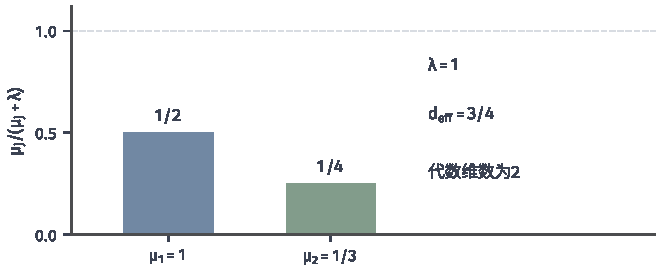
\includegraphics[width=112mm]{figures/01-mathematical-preliminaries-upper/02-linear-algebra-and-geometry/matplotlib/comprehension-additions/functional-effective-dimension-soft-count.pdf}
  \caption{有效维度按收缩比例计数。仿射核的两个正特征值为$1$和$1/3$，固定$\lambda=1$时，两个柱高分别为$1/(1+1)=1/2$与$(1/3)/(1/3+1)=1/4$，总和为$d_{\mathrm{eff}}=3/4$。灰虚线标记单一方向的完整贡献$1$，不表示另一项估计结果。}
  \label{fig:vol1-add-functional-effective-dimension}
\end{figure}

\subsubsection{固定参数下的数据稳定性}
\label{subsubsec:whole-fit-data-stability}

固定核、测度和$\lambda>0$，比较两个不同目标$y,\tilde y$对应的精确解$f_\lambda,\tilde f_\lambda$。对目标之差作相同的$L^2$谱分解：$y-\tilde y=\sum_j\delta c_j\psi_j$（零谱部分被消去），则解之差为
\[
  f_\lambda-\tilde f_\lambda=\sum_j\frac{\mu_j\delta c_j}{\mu_j+\lambda}\psi_j.
\]
按$L^2$范数计量，正谱系数乘上$\mu_j/(\mu_j+\lambda)\le1$，故
\[
  \|f_\lambda-\tilde f_\lambda\|_{L^2}
  \le\|y-\tilde y\|_{L^2}.
\]
这个结论比较同一算子的两项输入，$\lambda$全程固定，不让参数同时变化。

若按$H$范数计量输出，系数另带$1/\mu_j$权重：
\[
  \|f_\lambda-\tilde f_\lambda\|_H^2
  =\sum_j\frac{\mu_j\,\delta c_j^2}{(\mu_j+\lambda)^2}
  \le\frac{1}{4\lambda}\sum_j\delta c_j^2
  =\frac{\|y-\tilde y\|_{L^2}^2}{4\lambda},
\]
最后一步用$\mu_j/(\mu_j+\lambda)^2\le1/(4\lambda)$。于是
\begin{equation}
  \|f_\lambda-\tilde f_\lambda\|_H
  \le\frac{\|y-\tilde y\|_{L^2}}{2\sqrt\lambda}.
  \label{eq:functional-whole-fit-h-stability}
\end{equation}
换范数后常数从一变成$1/(2\sqrt\lambda)$，说明计量空间改变后实际改变了什么，而不是直接搬用前一段的系数一。

这里的数据稳定性、上一项的参数极限、以及有限任务中的算法误差各有各自的固定量与变化量：数据稳定性固定$K,\mu,\lambda$而改变$y$；参数极限固定$y,K,\mu$而改变$\lambda$；算法误差固定$y,K,\mu,\lambda$而增加迭代次数。一个任务既可能数据稳定又难以计算，也可能在$\lambda\downarrow0$时失去统一稳定常数，不能以其中一项代替另外两项。

\subsection{梯度场拟合与边界条件}
\label{subsubsec:gradient-field-fitting}

这里把观测从函数值改为向量场$v$：希望未知$u$的梯度接近$v$。固定有界连通Lipschitz域$\Omega\subset\mathbb R^d$，观测向量场$v\in L^2(\Omega;\mathbb R^d)$，已给提升$G\in H^1(\Omega)$与边界数据$g=\operatorname{Tr}G$（迹算子见第~\ref{subsubsec:trace-zero-boundary}节）。候选为
\[
  C=G+H_0^1(\Omega).
\]
残差是$\nabla u-v$；$v$未必是某个标量函数的精确梯度（例如环流场），因此不先假定残差可消为零，目标只能是“尽量小”。

\subsubsection{残差密度与可行扰动}
\label{subsubsec:residual-density-feasible}

在同一$v,g,C$上写残差密度的一般形式
\[
  J_\rho(u)=\int_\Omega\rho(\nabla u-v)\,\mathrm dx.
\]
二次密度$\rho_2(r)=\|r\|^2/2$与幅度型密度
\[
  \rho_\varepsilon(r)=\sqrt{\|r\|^2+\varepsilon^2}
\]
只改变残差的计价方式，不改变观测类型。它们可以与函数值项或有限读数项组合，但组合后必须重新写出完整目标、各项权重和共同候选，不能仅凭惩罚名称判断任务。

固定迹意味着允许扰动$h\in H_0^1(\Omega)$（边界迹为零）；若改为自由边界或均值约束，要先改变可行扰动集合，再使用共用的积分变分公式。$v=0$时上述两个密度才分别退化为纯梯度平方平滑与TV型平滑；没有其他观测或约束时，纯梯度平滑允许任意常量平移，不能说它自动保留信号。

\subsubsection{梯度残差的二次代价}
\label{subsubsec:quadratic-gradient-cost}

\paragraph{从二次目标到弱条件}

先取一维、$v=0$、固定端点的简单情形建立直觉：
\[
  J(f)=\frac12\int_0^1|f'|^2\,\mathrm dx.
\]
对光滑$f$和满足零端点条件的扰动$h$，展开
\[
  J(f+th)=\frac12\int|f'+th'|^2
  =J(f)+t\int f'h'\,\mathrm dx+\frac{t^2}{2}\int|h'|^2,
\]
故$DJ(f)[h]=\int f'h'\,\mathrm dx$。分部积分（$h$在端点为零，边界项消失）得$\int f'h'=-\int f''h$；由测试函数任意，驻点经典条件为$f''=0$，即仿射函数，再由固定端点值确定两个系数。一般$H^1$候选没有经典二阶导数时，先保留“对所有合法$h$成立”的积分条件$\int f'h'=0$，不强行点态化。注意这里是导数平方能量，要与二阶导数平方的弯曲能$\frac12\int|f''|^2$区别开：后者惩罚弯曲，前者惩罚斜率大小。

回到给定场$v\in L^2(\Omega;\mathbb R^d)$，取二次密度$\rho_2$（$v=0$时为$\frac12\int_\Omega\|\nabla u\|^2\,\mathrm dx$，即\term{Dirichlet能量}）：
\[
  J_2(u)=\frac12\int_\Omega\|\nabla u-v\|^2\,\mathrm dx.
\]
展开$J_2(u+th)-J_2(u)$的一次项（$h\in H_0^1$）：
\[
  t\int_\Omega(\nabla u-v)\cdot\nabla h\,\mathrm dx+o(t).
\]
故驻点弱式为
\begin{equation}
  \int_\Omega\nabla u\cdot\nabla h\,\mathrm dx
  =\int_\Omega v\cdot\nabla h\,\mathrm dx,
  \qquad\forall h\in H_0^1(\Omega).
  \label{eq:functional-guided-poisson-weak}
\end{equation}
当前$v\in L^2$和$u,h\in H^1$保证两边积分合法（Cauchy--Schwarz：$L^2$内$L^2$函数乘积可积）；即使$u$没有经典二阶导数，这个弱式仍保留。

在额外光滑条件下对左边分部积分，内部式解释为
\[
  \operatorname{div}(\nabla u-v)=0.
\]
自由边界处的自然通量是$(\nabla u-v)\cdot n$，一般不是齐次法向导数$\partial_nu=0$。若恰好$v=\nabla s$且$s\in H^1(\Omega)$，则$u-s$满足弱调和内部条件$\int\nabla(u-s)\cdot\nabla h=0$，边界差由修正项承担；任意$v$不必有这样的势$s$。

\paragraph{方程接口与求解边界}

这里的推导完成的是“候选与二次目标—可行一阶变化—弱方程”这条链路。带源Poisson方程、Poincaré不等式与Riesz表示下的存在唯一论证、自由边界的常量自由度以及源与通量相容条件，由后续微分方程章的Poisson弱解理论继续建立；本节不把当前驻点推导写成已经完成这些证明。连续弱问题存在唯一，也不能直接推出算法收敛或网格解逼近；具体五点系统及固定边界条件由五点差分承接，本章后面的连续能量离散节只检查已知函数的能量值和权重尺度，不替代解的数值分析。

\subsubsection{梯度残差的幅度代价}
\label{subsubsec:amplitude-gradient-cost}

\paragraph{正平滑参数下的一阶条件}

保留同一$v,g,C$，取$\varepsilon>0$及幅度型目标
\[
  J_\varepsilon(u)=\int_\Omega\sqrt{\|\nabla u-v\|^2+\varepsilon^2}\,\mathrm dx.
\]
先对残差向量$r=\nabla u-v$求密度导数：
\[
  \frac{\partial\rho_\varepsilon}{\partial r}
  =\frac{r}{\sqrt{\|r\|^2+\varepsilon^2}},
\]
再沿$\nabla h$用链式法则，得到一阶变化
\[
  \delta J_\varepsilon(u)[h]
  =\int_\Omega
  \frac{\nabla u-v}{\sqrt{\|\nabla u-v\|^2+\varepsilon^2}}
  \cdot\nabla h\,\mathrm dx.
\]
系数向量长度$\|\nabla u-v\|/\sqrt{\|\nabla u-v\|^2+\varepsilon^2}\le1$，被$|\nabla h|$一致支配，由控制收敛定理说明导数可以移入积分。令该一阶积分对全部合法$h\in H_0^1$为零，即得当前驻点弱条件；经典内部散度$\operatorname{div}\big((\nabla u-v)/\sqrt{\|\nabla u-v\|^2+\varepsilon^2}\big)=0$和自然边界通量，只在额外正则性或适用弱迹条件下解释。密度$\rho_\varepsilon$凸，故目标凸，但凸性不推出当前$H^1$候选中最小值达到或唯一，更不能沿用二次问题的Poisson线性形式。

\paragraph{零平滑参数、集中变化与BV边界}

当$\varepsilon=0$，残差为零处不能直接相除，应改用次梯度或变分不等式；$v=0$时密度退化为$\rho_0(r)=\|r\|$，即通常的\term{全变差}（TV）型平滑目标。用一个一维过渡比较两种密度对“集中变化”的响应：设$u$在宽度$\delta$内从高度$0$线性过渡到高度$a$，其余处斜率为零，则
\[
  \begin{aligned}
    \text{幅度积分}&=\int|u'|\,\mathrm dx=\frac{|a|}{\delta}\cdot\delta=|a|,\\
    \text{二次能量}&=\frac12\int|u'|^2\,\mathrm dx
      =\frac12\left(\frac a\delta\right)^2\delta=\frac{a^2}{2\delta}.
  \end{aligned}
\]
过渡收窄（$\delta\to0$）时幅度积分保持$|a|$不变，二次能量按$1/\delta$发散。二者对同一过渡的不同响应完全来自密度本身：幅度密度对“总变化量”计价，二次密度对“变化速率平方”计价。

一维中具有非零高度的跳跃不属于当前$H^1$候选（$H^1$函数在一维有绝对连续代表，不允许跳）。若要允许跳跃，必须以分布导数的测度表示进入BV空间并重新规定目标；本节只指出这条范围边界，不把BV存在理论混写成当前$H^1$结论。多维中逐坐标绝对值之和与逐点欧氏长度是不同密度，前者对方向的计价不同。即便密度逐点积分，共享的未知函数和边界约束仍耦合各位置，优化不能逐点独立；与其他观测项组合时，还须重新核对可微性、次梯度和可行保持条件。
\section{有限表示与函数逼近}
\label{sec:finite-representation-approximation}

本节固定目标函数、允许的定义域和误差尺度，研究怎样用有限个生成单元及其组合得到一个函数。前文的有限观测表示定理是在给定目标和惩罚下删除不可见方向；这里则主动选择近似族，并比较表示规模、局部修改和可达到的误差。“存在一个近似表示”只回答这个族是否足够丰富，不替代由有限读数识别目标、寻找参数的算法或学习保证。

下面固定一个共同目标
\[
  f_*(x)=\left|x-\frac12\right|,\qquad x\in[0,1],
\]
贯穿全节：多项式可以随次数增加而一致逼近它，含$1/2$结点的线性样条可以精确表示它，两个ReLU单元也可以精确表示它。这个对照比较的是同一个函数所需的构造条件，不从三个例子推断某种方案对所有目标都更省规模。生成单元的选择与多变量的组合方式是两个可以叠加的设计问题，下面分别讨论，不把它们写成互斥的函数类型。

\subsection{生成单元的选择}
\label{subsubsec:choice-of-generating-units}

下面固定同一个定义域与误差口径，分别考察全局多项式、局部分段直线、固定宽度的高斯核截面和神经单元怎样生成近似函数。四种方案各有自己的固定对象与可变规模：多项式的次数、样条的结点、高斯核的中心与项数、神经单元的宽度，分别随目标和精度变化，误差结论依赖的条件也随之不同。它们是几种有明确构造的方案，彼此可能存在表示联系；例如高斯核稠密性的证明借助多项式，却并不使高斯核截面成为多项式的一类。

\subsubsection{多项式逼近}
\label{subsubsec:polynomial-approximation}

对$[0,1]$上的连续目标$f$，先给一个可直接由网格读数形成的多项式，再证明它怎样控制全区间误差。结论中的次数可以随目标和精度增加，不固定一个有限维多项式空间后就宣称它能逼近所有连续函数。

在展开估计之前，先固定两个全程使用的对象。

\begin{definition}[连续模]
设$f$在区间$I$上有界。对$\delta>0$，定义
\[
  \omega_f(\delta)=\sup_{\substack{s,t\in I\\|s-t|\le\delta}}|f(s)-f(t)|.
\]
它是$f$在长度$\delta$的尺度上的最大振幅。$f$在紧区间上一致连续，等价于$\omega_f(\delta)\to0$（$\delta\downarrow0$）；若$f$还满足$|f(s)-f(t)|\le L|s-t|$，则有$\omega_f(\delta)\le L\delta$。
\label{def:functional-continuity-modulus}
\end{definition}

\paragraph{Bernstein多项式的构造}

固定整数$m\ge1$，在结点$j/m$读取$f$，定义
\begin{equation}
  B_mf(x)=\sum_{j=0}^{m}f\!\left(\frac jm\right)w_{m,j}(x),
  \qquad
  w_{m,j}(x)=\binom mjx^j(1-x)^{m-j}.
  \label{eq:functional-bernstein-polynomial}
\end{equation}
结点值是已知输入，$x$是求近似值的位置；每个权重都是$x$的多项式，因此结果仍是次数至多$m$的多项式。

把$m$个$x+(1-x)$的有限乘积按“选中$x$的次数”分组，得到
\[
  \sum_jw_{m,j}(x)=\bigl(x+(1-x)\bigr)^m=1;
\]
在$0\le x\le1$上各权重非负，因此$B_mf(x)$是结点值的凸组合。这一步只用有限乘积和二项式展开，不预先调用概率论。凸组合说明了取值范围，却还没有说明主要权重是否集中在靠近$x$的结点；下面把这个位置问题算成一组有限和恒等式。

\begin{lemma}[Bernstein权重的矩]
对$0\le x\le1$，上述权重满足
\[
  \sum_{j=0}^m w_{m,j}(x)=1,\qquad
  \sum_{j=0}^m j\,w_{m,j}(x)=mx,
\]
以及
\[
  \sum_{j=0}^m j(j-1)w_{m,j}(x)=m(m-1)x^2.
\]
进而有二阶中心矩恒等式
\begin{equation}
  \sum_{j=0}^m\left(\frac jm-x\right)^2w_{m,j}(x)
  =\frac{x(1-x)}m\le\frac1{4m}.
  \label{eq:functional-bernstein-second-moment}
\end{equation}
\end{lemma}

\begin{proof}
第一式已由二项式定理给出。对第二式，利用$j\binom mj=m\binom{m-1}{j-1}$，把求和下标改为$k=j-1$：
\[
  \sum_{j=0}^m j\,w_{m,j}(x)
  =mx\sum_{k=0}^{m-1}\binom{m-1}{k}x^k(1-x)^{m-1-k}
  =mx.
\]
对第三式，再用$j(j-1)\binom mj=m(m-1)\binom{m-2}{j-2}$（$m=1$时左边直接为零），类似地把下标改为$k=j-2$，得到
\[
  \begin{aligned}
  \sum_{j=0}^m j(j-1)w_{m,j}(x)
  &=m(m-1)x^2
    \sum_{k=0}^{m-2}\binom{m-2}{k}x^k(1-x)^{m-2-k}\\
  &=m(m-1)x^2.
  \end{aligned}
\]
最后用$j^2=j(j-1)+j$展开二阶中心矩：
\[
  \sum_j(j/m-x)^2w_{m,j}
  =\frac1{m^2}\sum_jj^2w_{m,j}-\frac{2x}{m}\sum_jj\,w_{m,j}+x^2\sum_jw_{m,j}.
\]
代入前两式，即得$(m(m-1)x^2+mx)/m^2-2x^2+x^2=x(1-x)/m$；再由$x(1-x)\le1/4$（$0\le x\le1$）得到右端上界$1/(4m)$。
\end{proof}

这个有限和恒等式的意义是：权重虽然散布在全部结点上，但离$x$较远的结点所占的总权重受$1/(4m)$控制，因而随$m$增大而衰减。

\paragraph{一致误差的估计}

\begin{theorem}[Bernstein--Weierstrass逼近]
设$f\in C([0,1])$，$B_mf$为式~\eqref{eq:functional-bernstein-polynomial}的Bernstein多项式。对任意$\delta>0$，
\begin{equation}
  \|B_mf-f\|_\infty
  \le\omega_f(\delta)+\frac{\|f\|_\infty}{2m\delta^2}.
  \label{eq:functional-bernstein-error}
\end{equation}
因而$\|B_mf-f\|_\infty\to0$（$m\to\infty$）。
\end{theorem}

\begin{proof}
固定$\delta>0$，用权重和为一把差写成
\[
  B_mf(x)-f(x)
  =\sum_{j=0}^m\left[f\!\left(\frac jm\right)-f(x)\right]w_{m,j}(x).
\]
把结点分成近处$|j/m-x|\le\delta$与远处$|j/m-x|>\delta$两组，这是同一个误差的两部分，并未另换目标或误差范数。

近处每个差值至多为连续模$\omega_f(\delta)$，而近处权重之和不超过$1$，故近处贡献不超过$\omega_f(\delta)$。

远处对每个$j$用$1\le(j/m-x)^2/\delta^2$放大权重，再由上面的矩恒等式控制总权重：
\[
  \sum_{|j/m-x|>\delta}w_{m,j}(x)
  \le\frac1{\delta^2}\sum_{j=0}^m\left(\frac jm-x\right)^2w_{m,j}(x)
  \le\frac1{4m\delta^2}.
\]
远处再用$|f(j/m)-f(x)|\le|f(j/m)|+|f(x)|\le2\|f\|_\infty$，得到远处贡献不超过$\|f\|_\infty/(2m\delta^2)$。两部分相加即得式~\eqref{eq:functional-bernstein-error}。

最后，$f$在紧区间$[0,1]$上一致连续，故任给$\varepsilon>0$可先选$\delta$使$\omega_f(\delta)<\varepsilon/2$；保持这个$\delta$，再取足够大的$m$使$\|f\|_\infty/(2m\delta^2)<\varepsilon/2$。两步缺一不可：仅知道某个固定$x$处误差趋零，不足以得出全区间共用的结论。
\end{proof}

回到折点目标$f_*$，本定理保证任意精度的一致多项式逼近，但任意一个多项式在$1/2$处都可微，不能与$f_*$在整个区间上完全相同。一般连续性也没有给出所有连续目标共用的快速速率；上面的速率$\omega_f(\delta)+C/(m\delta^2)$只说明收敛，常数随$\delta$的选择而变。下一个方案利用分段结构，在特定结点条件下直接表示这个折点。

\subsubsection{样条逼近}
\label{subsubsec:spline-approximation}

样条以分段多项式和指定结点衔接条件定义。这里先取最简单的连续分段直线，研究结点值怎样生成局部插值，以及结点变密怎样控制同一个连续目标的误差。

\paragraph{线性样条的构造与误差}

固定
\[
  0=t_0<t_1<\cdots<t_N=1,
\]
结点值$f(t_i)$及最大间距$h=\max_i(t_{i+1}-t_i)$。对$x\in[t_i,t_{i+1}]$写
\begin{equation}
  S_hf(x)=(1-s)f(t_i)+sf(t_{i+1}),
  \qquad s=\frac{x-t_i}{t_{i+1}-t_i}.
  \label{eq:functional-linear-spline}
\end{equation}
相邻区间在公共结点使用同一个读数，所以这个构造给出连续分段直线。要先区分“由全部样条组成的候选空间”与“由结点数据产生当前插值函数的操作”。

\begin{theorem}[线性样条的插值误差]
在上述记号下，若$f$在$[0,1]$上连续，则
\begin{equation}
  \|f-S_hf\|_\infty\le\omega_f(h).
  \label{eq:functional-spline-modulus-error}
\end{equation}
若再有$f\in C^2([0,1])$，则
\begin{equation}
  \|f-S_hf\|_\infty\le\frac{h^2}{8}\|f''\|_\infty.
  \label{eq:functional-spline-quadratic-error}
\end{equation}
\end{theorem}

\begin{proof}
在单元$[t_i,t_{i+1}]$上，由$(1-s)+s=1$把$f(x)-S_hf(x)$拆成
\[
  f(x)-S_hf(x)=(1-s)\bigl(f(x)-f(t_i)\bigr)+s\bigl(f(x)-f(t_{i+1})\bigr).
\]
两个端点离$x$都不超过$h$：$|x-t_i|=s(t_{i+1}-t_i)\le h$，$|x-t_{i+1}|=(1-s)(t_{i+1}-t_i)\le h$。故
\[
  |f(x)-S_hf(x)|\le(1-s)\omega_f(h)+s\omega_f(h)=\omega_f(h).
\]
对全部区间取上确界即得式~\eqref{eq:functional-spline-modulus-error}。若一列网格的最大间距$h\to0$，一致连续性使$\omega_f(h)\to0$，这些插值函数便一致趋于$f$；这个结论不要求网格等距。

为得到二阶速率，固定一个单元并考虑$g(x)=f(x)-S_hf(x)$。它在两端$t_i,t_{i+1}$处为零。对任意$x\in(t_i,t_{i+1})$，令
\[
  \lambda=\frac{g(x)}{(x-t_i)(x-t_{i+1})},
  \qquad
  G(u)=g(u)-\lambda(u-t_i)(u-t_{i+1}).
\]
函数$G$在$t_i,t_{i+1},x$三点处都为零。由Rolle定理，$G'$在这三点两两之间各有一个零点，共两个零点；再用一次Rolle定理，$G''$在单元内某点$\xi$处为零。注意$S_hf$在单元内是一次多项式，$S_h''=0$，而$((u-t_i)(u-t_{i+1}))''=2$，故
\[
  0=G''(\xi)=f''(\xi)-2\lambda,
  \qquad
  \lambda=\frac{f''(\xi)}2.
\]
代回$\lambda$的定义，得余项表示
\[
  f(x)-S_hf(x)=\frac{f''(\xi)}2(x-t_i)(x-t_{i+1}).
\]
在单元上$|(x-t_i)(x-t_{i+1})|\le\bigl((t_{i+1}-t_i)/2\bigr)^2\le h^2/4$，因而$|f(x)-S_hf(x)|\le h^2\|f''\|_\infty/8$。对单元取上确界即得式~\eqref{eq:functional-spline-quadratic-error}。新增的二阶导数条件支持更具体的速率，不能由一般连续性直接取得。
\end{proof}

\paragraph{样条的示例与局部修改}

\begin{example}[二次函数的两段插值]
对$f(x)=x^2$只取结点$0,1$，由端点值$0,1$得到$S_hf(x)=x$。函数$x-x^2$在$x=1/2$处取最大值$1/4$，故误差恰为$1/4$。此时$h=1$、$\|f''\|_\infty=2$，上一界$h^2\|f''\|_\infty/8=2/8=1/4$，二者吻合，可供核对余项估计中的常数。
\end{example}

对折点目标$f_*$，若结点包含$0,1/2,1$，则$[0,1/2]$上的直线斜率为$-1$、$[1/2,1]$上的斜率为$+1$，与$f_*$两侧斜率相同，因此已能精确表示。它与多项式方案比较的是同一目标在不同生成规则下的表示条件，并不说明某个固定结点集合能精确表示任意连续目标。

固定其他结点值、只改变一个内部结点的值时，当前线性插值公式只在相邻两段改变，这种局部性来自帽形生成函数的支撑；误差界则来自端点凸组合，两种结论使用不同依据。图~\ref{fig:functional-basis-locality}把三类生成单元在同一结点$1/2$处取单位系数放在一起比较，可见局部支撑与全局基的差别。提高样条次数或改成多变量张量积后，要重新检查衔接、插值与系数依赖，不能把“局部分段”直接当成全部性质的保证。

\begin{center}
\begin{minipage}{\linewidth}
 \centering
 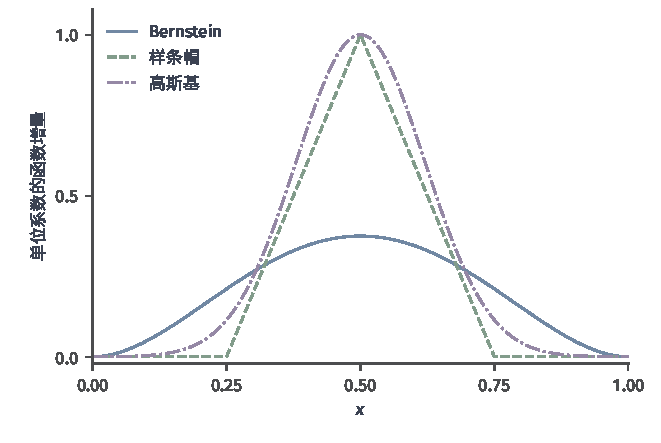
\includegraphics[width=112mm]{figures/01-mathematical-preliminaries-upper/02-linear-algebra-and-geometry/matplotlib/teaching-analysis/functional-basis-locality.pdf}
 \functionalinlinefigurecaption{fig:functional-basis-locality}
   {同一结点$1/2$处取单位系数的三类生成单元。Bernstein权重（实线）在整个$(0,1)$上非零，峰值远小于$1$；线性样条帽形函数（虚线）只在相邻两段$[1/4,3/4]$上非零，即局部支撑；高斯核截面（点划线）光滑衰减但处处非零。改变一个内部结点值只影响帽形基所在两段插值，这种局部性来自生成函数的支撑，与插值误差的凸组合界依据不同；全局基的系数依赖范围也随之更宽。}
\end{minipage}
\end{center}

\subsubsection{固定宽度高斯核截面的逼近}
\label{subsubsec:gaussian-section-approximation}

现在保持每个生成单元的宽度不变，只允许中心、线性系数和项数变化。要证明这套单元也能逼近连续目标，需要把核截面的有限和与前面的多项式逼近联系起来；证明中借助多项式，但所得近似器仍是高斯核截面的有限和。

\paragraph{固定宽度的核截面与中心差分}

在$[0,1]$固定$\sigma>0$，取
\[
  K_\sigma(x,c)=\exp\left(-\frac{(x-c)^2}{2\sigma^2}\right),
\]
并允许所有中心$c\in[0,1]$。候选近似器为
\[
  \sum_{\ell=1}^{M}a_\ell K_\sigma(\cdot,c_\ell),
\]
其中$M$和实系数可以变化；这里的稠密性采用一致范数，不对系数大小或核空间范数预设统一预算。

固定内部中心$c_0=1/2$，令$w(x)=K_\sigma(x,c_0)$。对中心连续求导：一阶导数为$\partial_cK_\sigma(x,c)=(x-c)K_\sigma(x,c)/\sigma^2$，它仍含因子$w(x)$；逐次求导便归纳地得到
\begin{equation}
  \partial_c^jK_\sigma(x,c_0)=w(x)P_j(x),
  \label{eq:functional-gaussian-derivative-polynomial}
\end{equation}
其中$P_j$是次数$j$的多项式，最高次项系数为$\sigma^{-2j}$。归纳步骤是：对$w(x)P_j(x)$再关于$c$求一次导，新增项$(x-c)wP_j/\sigma^2$只把最高次数提高一次，且首项系数乘$\sigma^{-2}$。

对每个固定$j$，取足够小的$h>0$，使$c_0,c_0+h,\ldots,c_0+jh$都在合法中心域内，写中心$j$阶前向差分
\begin{equation}
  h^{-j}\sum_{\ell=0}^{j}(-1)^{j-\ell}\binom j\ell
  K_\sigma(x,c_0+\ell h).
  \label{eq:functional-center-forward-difference}
\end{equation}
这是$j$个核截面的有限线性组合。由$\partial_c^jK_\sigma$在紧矩形$[0,1]\times[c_0-\varepsilon,c_0+j\varepsilon]$上连续，有限差分对全部$x$一致收敛到导数~\eqref{eq:functional-gaussian-derivative-polynomial}。因此每个$wP_j$都属于核截面有限和的一致闭包；不能只从逐点求导就直接宣称一致逼近，一致性来自差分在$x$上的一致收敛。

\paragraph{从加权多项式到一致稠密性}

\begin{theorem}[固定宽度高斯核截面的一致稠密性]
设$\sigma>0$固定，则全体有限和$\sum_{\ell=1}^{M}a_\ell K_\sigma(\cdot,c_\ell)$（$M$、$a_\ell$、$c_\ell$均可随目标变化）在$C([0,1])$的一致范数下稠密。
\end{theorem}

\begin{proof}
分三步。

第一步，把多项式方向并入闭包。$P_j$的最高次项非零（系数$\sigma^{-2j}\ne0$），故$P_0,P_1,\ldots,P_m$与单项式$1,x,\ldots,x^m$之间的系数变换是对角元非零的上三角变换。逐次消去最高次数，就能把任意次数至多$m$的多项式$P$写成$P_0,\ldots,P_m$的有限线性组合。于是每个加权多项式$wP$也属于核截面有限和的一致闭包。

第二步，把目标折成加权多项式。$w$在紧区间$[0,1]$上连续且严格为正，故有正下界；$f$连续时$f/w$仍连续。对$f/w$用已证明的Bernstein--Weierstrass定理，可找多项式$P$使$\|f/w-P\|_\infty$任意小，即$\|f-wP\|_\infty$任意小。

第三步，把$wP$换成真正的有限核和。把$P=\sum_j c_jP_j$写成有限组合；对每个固定$j$，由中心差分~\eqref{eq:functional-center-forward-difference}选足够小的步长，使该$wP_j$的一致逼近误差任意小。最后用三角不等式合并“$f$到$wP$”与“$wP$到有限核和”两类误差，便得到一个项数有限的高斯核截面和，其一致误差小于任意给定精度。
\end{proof}

项数和中心可以随目标及精度变化，是上述结论的条件。若只允许一个预先固定的有限中心集合，所得有限维张成在$C([0,1])$中是闭的且不等于整个空间，便不具有这种稠密性；差分中的小步长还可能带来大系数，证明不提供统一的规模、数值稳定或寻参保证。固定宽度高斯核在紧集上的通用性可与Steinwart的原论文核对\scite{steinwart2001kernel}；这里展开的是一维区间上的具体证明路线。

\subsubsection{神经网络逼近}
\label{subsubsec:neural-network-approximation}

神经单元把输入的仿射变换送入激活函数，再由有限线性组合形成输出。先对共同折点目标直接计算，再区分这个小构造与“对所有连续目标”的存在定理。

\paragraph{折点函数的两单元表示}

\begin{example}[折点函数的两ReLU表示]
定义$\operatorname{ReLU}(s)=\max(s,0)$。对$f_*(x)=|x-1/2|$，直接写
\[
  \operatorname{ReLU}\!\left(x-\frac12\right)
  +\operatorname{ReLU}\!\left(\frac12-x\right).
\]
当$x\ge1/2$时第一项为$x-1/2$、第二项为零；当$x\le1/2$时第一项为零、第二项为$1/2-x$；两端合并恰为$|x-1/2|$。分两侧核对后可见：两个输入权重取正负号、偏置都放在折点$1/2$、输出相加，各自的作用都不可省略。
\end{example}

这个单隐藏层构造使用两个ReLU单元，不要求训练过程就能验证其表示。它与线性样条共用同一折点目标是为了比较生成规则；一个简单函数有小网络，并不推出任意目标都有同样规模，也不由两侧计算推出通用逼近定理。

\paragraph{通用逼近的条件与边界}

\begin{theorem}[单隐藏层通用逼近]
固定非空紧集$X\subset\mathbb R^d$、$f\in C(X)$和连续且不是多项式的激活函数$\sigma$。采用含偏置的单隐藏层形式
\begin{equation}
  c+\sum_{j=1}^{M}a_j\sigma(w_j^{\top}x+b_j).
  \label{eq:functional-universal-approximation}
\end{equation}
则对每个$\varepsilon>0$，可以选择有限的$M$与实参数$c,a_j,w_j,b_j$，使式~\eqref{eq:functional-universal-approximation}在$X$上与$f$的一致误差小于$\varepsilon$。
\end{theorem}

这一连续激活版本由Leshno等人的结果支持\scite{leshno1993approximation}；这里陈述的是存在定理，不伪装成已经给出针对一般目标的构造算法。

用Sigmoid、Tanh和ReLU核对“连续且非多项式”的条件，可知定理不要求激活处处可微。反之，若激活是固定次数$r$的多项式，同一单隐藏层形式无论增加多少单元：仿射变换$w_j^\top x+b_j$代入$r$次多项式后仍是次数至多$r$的多项式，有限线性组合后输出次数仍至多$r$。这种固定次数空间不能在有非空内部的紧域上逼近所有连续目标（例如$x^{r+1}$在一个小区间上的行为）。因此“用了非线性”不足以替代非多项式条件，偏置也属于这里采用的定理形式。

一致误差控制全部输入位置；转为$L^2(\mu)$误差时，还要给出测度及有限总质量，才能使用
\[
  \|f-g\|_2=\left(\int_X|f-g|^2\,\mathrm d\mu\right)^{1/2}
  \le\mu(X)^{1/2}\|f-g\|_\infty.
\]
反向可能受小区域尖峰阻碍：$L^2$小而一致误差大的函数对是存在的。由评价对象不同可以说明两个逼近命题的联系与边界，同时保留这些限制：通用逼近不保证最小宽度、参数可由有限读数识别、训练收敛或泛化。

\subsection{多变量函数的组合}
\label{subsubsec:multivariable-composition}

输入分为$p,q$两组后，可以把单组函数组合成有限乘积和
\[
  F_r(p,q)=\sum_{j=1}^{r}u_j(p)v_j(q);
\]
多项式、样条或神经单元都可作为因子的构造方式。这里研究的是变量如何共同作用，改变了上一分支中“只选生成单元”的问题；项数$r$与因子幅度仍须分别记录。

下面按实际任务区分：已给整个目标函数时，构造分离近似并控制全域误差；已给规则网格读数时，构造符合这些读数的\term{张量积插值}。两者不是互斥的结构类型，网格系数也可以具有低秩；“没有指定网格读数”不是低秩的定义。先确定共同乘积结构，再说明各任务额外固定的数据和评价条件。

\subsubsection{给定函数的分离近似}
\label{subsubsec:separated-approximation}

固定整个二维目标后，问少量单组因子的乘积之和能否在整个定义域上控制误差。所构造的项数给出一个可行表示规模，不自动给出所有同规模表示中的最优误差。

\paragraph{指数函数的分离构造}

固定$E(p,q)=e^{pq}$及$(p,q)\in[-1,1]^2$，取
\begin{equation}
  E_r(p,q)=\sum_{k=0}^{r-1}\frac{p^kq^k}{k!}.
  \label{eq:functional-separated-taylor}
\end{equation}
逐项写成只依赖$p$的$p^k/k!$与只依赖$q$的$q^k$的乘积；这个Taylor构造因此使用至多$r$个分离项，不能只因它写成一个二维多项式，就跳过变量分组的识别。

因$|pq|\le1$，把$pq$看作一元变量$t$，一元指数Taylor余项给出
\[
  |e^{pq}-E_r(p,q)|\le\frac{e^{|pq|}|pq|^r}{r!}\le\frac{e}{r!}.
\]
对整个正方形取上确界后仍有相同上界，故增加项数给出一致逼近；这是一条可行截断序列的保证，并未证明它在所有$r$项分离表示中最优。

再固定$q=1$观察$r=1,2,4$：对应截面分别为$1$、$1+p$、$1+p+p^2/2+p^3/6$，在$p=1$处的误差可直接核对为$e-1$、$e-2$和$e-8/3$（即$e-8/3\approx0.052$）。这些截面与具体点值帮助解释展开过程，整个定义域上的保证仍由上一段余项估计给出。图~\ref{fig:vol1-add-functional-separated-taylor-remainder}沿$q=1$截面展示余项，不要求读者另看图片才理解界。

\begin{figure}[!htb]
  \centering
  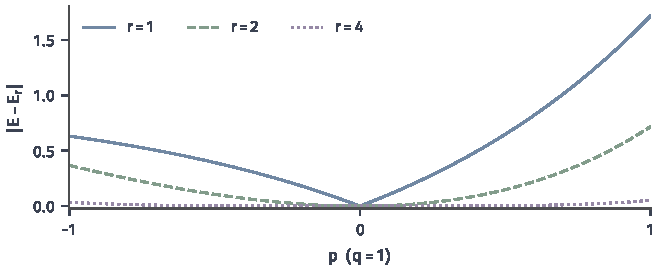
\includegraphics[width=112mm]{figures/01-mathematical-preliminaries-upper/02-linear-algebra-and-geometry/matplotlib/comprehension-additions/functional-separated-taylor-remainder.pdf}
  \caption{分离表示的截断余项。目标为$E(p,q)=e^{pq}$，$E_r$保留$k=0,\ldots,r-1$共$r$项，图中固定$q=1$并比较$r=1,2,4$的绝对误差$|E-E_r|$；三条曲线在$p=0$处均为零，随$|p|$增大而上升，$r$越大误差越小。所有曲线由解析式计算。正文界$e/r!$对整个$[-1,1]^2$成立；这里没有声称Taylor截断是最佳秩$r$逼近。}
  \label{fig:vol1-add-functional-separated-taylor-remainder}
\end{figure}

\paragraph{分离项的尺度与适用范围}

把$r$个因子分别组成向量$u(p)$与$v(q)$，其第$j$个分量为$u_j(p)$与$v_j(q)$，由Cauchy--Schwarz得
\[
  |F_r(p,q)|=\left|\sum_{j=1}^ru_j(p)v_j(q)\right|
  \le\|u(p)\|_2\|v(q)\|_2.
\]
项数说明表示用了多少个分离方向，因子范数控制这些方向的幅度；相同项数并不限制输出大小，也不独自控制函数类在指定误差下的覆盖数。某些Bellman残差矩阵也使用两个因子内积的形式，可据此辨认结构上的类比；但矩阵条目的含义、可实现性、查询协议与样本结论都依赖相应决策任务。这里不从$e^{pq}$的Taylor误差或一般因子界推出强化学习保证，函数类的统一代表数量留给覆盖数任务另行定义。

\subsubsection{网格数据的张量积插值}
\label{subsubsec:tensor-grid-interpolation}

现在不预先给出整个目标，只固定单位整数网格上的样本值$U_{ij}$，希望在非整数位置求值且经过原有网格读数。共同形式是
\begin{equation}
  S(x,y)=\sum_{i,j}c_{ij}h(x-i)h(y-j);
  \label{eq:functional-tensor-interpolation}
\end{equation}
一维核决定每轴的衔接与支撑，系数如何由样本产生则是另一项必须核对的条件。有限网格须指定边界延拓；下面B样条的可逆论证明确采用周期边界，不能自动移给其他端点条件。

三种方案在同一任务下比较结点插值、导数连续、取值范围和计算依赖：双线性和三次卷积可以直接用样本作系数；三次B样条则要先恢复系数再局部求值。这个差别在选择局部核时就必须注意，不能以“都具有有限支撑”掩盖样本到系数的过程。

\paragraph{双线性插值}

定义帽核$h(s)=\max(1-|s|,0)$，核对$h(0)=1$、非零整数处为零（基数条件）。取$c_{ij}=U_{ij}$时，整数网格位置$(i,j)$只留下对应的一个样本$U_{ij}$，因此满足插值；二维形式由两轴核的乘积生成。

对查询$(x,y)=(i+s,j+t)$、$s,t\in[0,1]$，只有四个核同时非零，展开权重
\[
  (1-s)(1-t),\quad s(1-t),\quad (1-s)t,\quad st
\]
及其对应四角样本$U_{i,j},U_{i+1,j},U_{i,j+1},U_{i+1,j+1}$。每项非负且总和为一，所以输出落在这四个样本的最小值和最大值之间；范围保持来自凸组合，而非来自“线性”这个名称。固定一个坐标时输出关于另一坐标线性；共同展开一般含$st$交叉项，所以通常不是整个平面上的仿射函数。相邻单元在公共边使用同一线性插值，函数值能够衔接，一阶导数一般会跳变；这也明确了更换核所要改善的是哪一种连续性。给定边界延拓后，每次求值只用所在单元四角样本，也可先沿一轴再沿另一轴计算。

\paragraph{三次卷积插值}

令$r=|s|$，定义Keys核：
\[
  h_a(s)=
  \begin{cases}
    (a+2)r^3-(a+3)r^2+1,&0\le r\le1,\\
    ar^3-5ar^2+8ar-4a,&1<r<2,\\
    0,&r\ge2.
  \end{cases}
\]
先检查衔接：$r=1$处左段值$(a+2)-(a+3)+1=0$、右段值$a-5a+8a-4a=0$，两侧一阶导数分别为$3(a+2)-2(a+3)=a$与$3a-10a+8a=a$，故函数值与一阶导数都连续；$r=2$处右段值$8a-20a+16a-4a=0$、导数$12a-20a+8a=0$，与外侧零相接；原点处两段关于$|s|$对称。综合得到$C^1$衔接和有限支撑$[-2,2]$；整数处的基数条件使样本仍能直接作系数。

对单位单元内位置$s\in[0,1]$，四个非零结点$-1,0,1,2$的权重为
\[
  h_a(s+1),\ h_a(s),\ h_a(s-1),\ h_a(s-2).
\]
把对应分段式展开相加得到一；再将两轴权重和相乘传到二维，便取得常量保持。这个计算不要求各权重非负，因此尚不能推出样本范围保持。

\begin{example}[半格查询的过冲]
取$a=-1/2$、查询半格$s=1/2$。由核的对称分段式算得四权重
\[
  \frac{(-1,\,9,\,9,\,-1)}{16}.
\]
若相应四个样本取$0,0,0,16$，则输出为$(-1\cdot0+9\cdot0+9\cdot0-1\cdot16)/16=-1$，越出样本区间$[0,16]$。这个直接可算的例子说明：$C^1$衔接与常量保持可以成立，同时仍发生过冲；二维张量积也不能仅靠提高衔接阶数取得范围保证。
\end{example}

二维每次求值至多使用$4\times4$个样本，此时系数就是样本，有限支撑确实对应直接样本的局部计算。这里不陈述未经额外光滑性和边界条件核对的全域误差阶。

\paragraph{三次B样条的系数恢复与求值}

定义中心\term{三次B样条}，令$r=|s|$：
\[
  \beta_3(s)=
  \begin{cases}
    \frac23-r^2+\frac12r^3,&0\le r<1,\\
    \frac16(2-r)^3,&1\le r<2,\\
    0,&r\ge2.
  \end{cases}
\]
核对分段处$r=1$的函数值（左段$2/3-1+1/2=1/6$，右段$(2-1)^3/6=1/6$）及一、二阶导数，均取得连续，故$\beta_3\in C^2$；再算
\[
  \beta_3(0)=\frac23,\qquad \beta_3(\pm1)=\frac16,\qquad \beta_3(\pm2)=0.
\]
这些整数值不满足直接用样本作系数所需的基数条件（$\beta_3(0)\ne1$、$\beta_3(1)\ne0$）。

先在一维写
\[
  S(x)=\sum_jc_j\beta_3(x-j),
\]
在整数结点代入得到
\begin{equation}
  S(i)=\frac{c_{i-1}+4c_i+c_{i+1}}6.
  \label{eq:functional-cubic-bspline-prefilter}
\end{equation}
若要求$S(i)=U_i$，必须先解这个“样本到系数”的线性系统；直接设$c_i=U_i$得到的是邻近样本的平滑累计，通常不会经过原样本。这样先看清不插值的原因，也就明白为什么需要系数恢复。

对长度$N$的周期网格，把下标按模$N$解释，并将周期正弦、余弦方向$c_j=e^{i\omega j}$代入上述卷积。频率$\omega=2\pi k/N$的响应为
\[
  \frac{e^{-i\omega}+4+e^{i\omega}}6=\frac{4+2\cos\omega}{6}\ge\frac{4-2}{6}=\frac13,
\]
所以所有周期方向上的响应非零，可唯一恢复系数；这一步也称预滤波。若改用其他边界规则，要先写出其端点方程再检查相应系统，不能沿用这个周期响应证明。二维样本到系数的关系是两个一维卷积沿两轴相继作用，因此先沿一轴恢复系数、再沿另一轴恢复，最后在查询点用张量积局部核求值。每个查询只访问邻近系数，但预滤波可能让一个原样本影响远处系数；因此“局部求值”与“结果只依赖邻近原样本”必须分别判断。

在单位单元内把四个非零B样条核权展开相加得到一；核权非负及其和为一至多把输出限制在“有关系数”的范围内，而系数已经过恢复，未必落在原样本取值范围，不能据此宣称原样本范围保持。回看三套方案，结点插值、$C^0/C^1/C^2$衔接、取值范围及计算依赖各有自己的核验依据。若后续缩小采样网格，还要按新的采样问题处理混叠；提高插值核阶数本身并不完成抗混叠。

\section{连续能量的离散逼近}
\label{sec:discrete-energy-approximation}

这里固定一个已知函数或一组函数记录，把连续积分目标改写成有限累计，研究权重、尺度和采样是否仍表达原来的量。它与“选择一个表示函数”不同，也与“重新求一个离散最优函数”不同；因此单独讨论能量值的逼近及扰动，不把这些结论并入拟合解稳定性。

本节按采样几何分为规则网格和一般点云；每种几何内部核对差分、积分权重与适用条件。点云分支在定义离散二次型后，还固定记录并核对边权变化怎样影响能量值，使扰动估计紧接其实际目标。

\subsection{规则网格的能量权重}
\label{subsubsec:regular-grid-energy}

\paragraph{从导数与积分尺度得到离散能量}

在$[0,1]$取
\[
  x_i=ih,\qquad i=0,\ldots,n,\qquad h=\frac1n,
\]
固定$f\in C^1([0,1])$。当前目标是
\[
  \frac12\int_0^1|f'|^2,
\]
网格值都来自同一个已知$f$，没有把节点值改成待求未知量。

邻点差先除以$h$才形成导数近似，平方后还要乘上积分单元长度$h$，所以定义
\begin{equation}
  E_h(f)=\frac1{2h}\sum_{i=0}^{n-1}\bigl[f(x_{i+1})-f(x_i)\bigr]^2.
  \label{eq:functional-grid-energy}
\end{equation}
要分别说明差商中的$h^{-2}$与积分中的$h$：单个差商$[f(x_{i+1})-f(x_i)]/h$近似导数，其平方乘单元长度$h$才是一个单元上的能量微元；合起来因子$1/(2h)$使最终权重的来源可复核，而不是把未归一化的邻差平方误当成同一能量。

\paragraph{已知函数的能量一致性}

\begin{theorem}[$E_h$的连续极限]
若$f\in C^1([0,1])$，则当$h\to0$时
\begin{equation}
  E_h(f)\to\frac12\int_0^1|f'(x)|^2\,\mathrm dx.
  \label{eq:functional-grid-energy-convergence}
\end{equation}
\end{theorem}

\begin{proof}
把差商写成局部导数平均：
\[
  \frac{f(x_{i+1})-f(x_i)}h=\frac1h\int_{x_i}^{x_{i+1}}f'(s)\,\mathrm ds.
\]
$f'$在紧区间上一致连续，故对单元内任意点$x_i+\theta h$，平均值与该点导数值之差不超过$\omega_{f'}(h)$；特别地，它与$|f'|^2$在单元上的代表值之差，在$f'$有界时被$\omega_{f'}(h)$与$\|f'\|_\infty$的乘积控制。于是
\[
  E_h(f)=\frac12\sum_{i=0}^{n-1}h\left(\frac{f(x_{i+1})-f(x_i)}h\right)^2
\]
与Riemann和$\frac12\sum_i h|f'(x_i)|^2$之差随$h\to0$趋于零；而$|f'|^2$连续，该Riemann和趋于$\frac12\int_0^1|f'|^2$。这里先处理同一函数的导数近似，再累计积分，两个步骤各有所需条件，不能只凭“网格变密”宣布极限。
\end{proof}

这个结论没有重新求最小者，因此不证明离散解逼近连续解。未知网格值的五点系统、固定边界唯一性以及足够光滑条件下的差分一致性，由后续微分方程章的五点差分处理；能量值一致、系统可解和解收敛必须分别建立。

\subsection{点云的能量权重与归一化}
\label{subsubsec:point-cloud-energy}

\paragraph{对称边权与点对计数}

给定固定标量记录$f_i$及对称非负边权
\[
  w_{ij}=w_{ji}\ge0,
\]
约定
\begin{equation}
  E_n(f)=\frac12\sum_{i,j=1}^nw_{ij}(f_i-f_j)^2
  \label{eq:functional-point-cloud-energy}
\end{equation}
遍历有序点对。非负性保证代价非负，对称性允许用无向边解释；对角项为零，每条非自环无向边则计了两次。

保持同一权重时，由对称性
\[
  E_n(f)=\sum_{i<j}w_{ij}(f_i-f_j)^2;
\]
若无向边“一次”的公式还带$1/2$，其有序和就应带$1/4$，或相应改变权重定义。要先核对求和对象，再比较系数和归一化，不能只凭表面的$1/2$判断两个目标相同或不同。

\paragraph{离散累计何时具有连续解释}

规则网格曾提供单元长度和邻点距离，点云却没有自动给出这些量。若要把式~\eqref{eq:functional-point-cloud-energy}解释为连续梯度能量的近似，必须另给采样密度、邻近半径、核权、样本规模的归一化以及目标函数的正则性，并说明它们怎样把局部差平方变成积分。

条件没有给全时，只能把$E_n$视为一个合法的离散二次目标，不宣称任意图能量都收敛到某个连续几何能量。当前标量记录能够直接相减；若记录为不同点的切向量，还必须规定跨点比较或搬运，相关联络条件由流形章建立。

\paragraph{离散能量值的扰动界}

固定$f_i$、有序点对与前面的系数约定，把权重改为$\widetilde w_{ij}$，记
\[
  \delta w_{ij}=\widetilde w_{ij}-w_{ij}.
\]
直接相减两个目标、逐项取绝对值，得到
\begin{equation}
  |\widetilde E_n(f)-E_n(f)|
  \le\frac12\sum_{i,j=1}^n|\delta w_{ij}|(f_i-f_j)^2.
  \label{eq:functional-energy-weight-perturbation}
\end{equation}
若新旧目标都要求非负能量，还应各自核对边权非负。右端同时取决于权重差和当前记录的邻点差，不能只看边权变了多少而忽略所评价的函数。这个上界控制的是同一记录的目标值，既没有重新最小化，也没有比较两个最优函数，因此不能当成解稳定定理。

\paragraph{目标权重与计算内积的区别}

若这些边权进入目标二次型，改变权重就改变了最优化问题；若目标保持不变，只改变用于表示微分的内积，则目标最优者不因此改变，梯度和演化方向却会改变。可以回用前面的仿射梯度例，明确“改权重”发生在哪个数学对象上。非负性只说明目标下界，不能替代扰动界、最小值达到或算法收敛。由此把本节能量值的稳定性与前面的有界运算、数据到最优函数的稳定性区分开，离散目标的条件留在其实际使用位置。

\section{函数类的覆盖数}
\label{sec:covering-numbers}

此前是为一个给定目标构造近似函数，或为一个拟合任务求解。这里改为固定整个非空函数类，问预先准备多少代表才能近似其中每个成员。这需要共同给定类、误差口径、精度和代表范围；单个目标可逼近、参数个数有限或谱有效维度有限，都不能直接代替这个问题。

本节按评价输入是否预先固定，分为普通覆盖与依历史变化的查询树覆盖。它们改变的是评价协议和代表对象，不能仅按阅读先后把后者说成前者的同一距离。

\subsection{固定距离下的覆盖数}
\label{subsubsec:covering-number-fixed}

\paragraph{距离、代表集合与量词}

\begin{definition}[固定距离下的覆盖数]
固定非空类$\mathcal F$、距离或伪距离$d$和精度$\delta>0$，先约定代表属于$\mathcal F$。有限集$V\subseteq\mathcal F$若对所有$f\in\mathcal F$都存在$v\in V$使
\[
  d(f,v)\le\delta,
\]
就构成一个$\delta$-覆盖；用最少代表数定义
\begin{equation}
  N(\delta,\mathcal F,d),
  \label{eq:functional-covering-number}
\end{equation}
无有限覆盖时记为无穷。若允许类外中心，必须另行说明该约定，不能无声改变数值口径。
\end{definition}

代表集必须在选定待近似成员之前固定，并覆盖所有成员；平均只对某些函数近似良好不能满足要求。全域上确界、指定测度的$L^2$误差和固定样本上的均方根是不同口径；经验误差可能为零而域外函数不同，因此通常只是伪距离。

覆盖数中的最坏要求针对类中每个函数，量词是“存在一个有限代表集，对所有函数存在近邻”：
\[
  \exists\,V\subset\mathcal F,\ \text{有限}\quad\text{s.t.}\quad
  \forall f\in\mathcal F,\ \exists v\in V:\ d(f,v)\le\delta.
\]
具体代表可以随函数选择，代表集则共同固定；先把允许集合与误差说清，再谈代表最少多少。图~\ref{fig:functional-covering-centers}在一个系数平面上展示覆盖的几何图景，正文随后对一个一维常值族给出显式估计。

\begin{center}
\begin{minipage}{\linewidth}
 \centering
 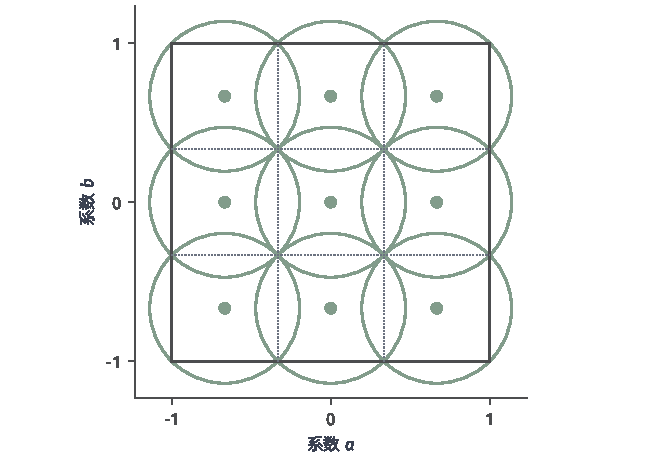
\includegraphics[width=112mm]{figures/01-mathematical-preliminaries-upper/02-linear-algebra-and-geometry/matplotlib/concepts-analysis-functional/covering-centers.pdf}
 \functionalinlinefigurecaption{fig:functional-covering-centers}
   {覆盖一个区域的几何图景。方形区域$[-1,1]^2$上，$9$个半径$\sqrt2/3$的圆盘中心排成$3\times3$网格$\{-2/3,0,2/3\}^2$；方形四角到最近中心的距离恰为$\sqrt2/3$，故整个方形被覆盖。代表数由区域在所选度量下的延伸和精度决定；正文对一维常值族给出显式估计$N\ge M/(2\delta)$。参数个数未变，区域尺度变大却使所需代表数增大。}
\end{minipage}
\end{center}

图~\ref{fig:functional-covering-centers}的系数平面并非抽象网格：它对应一元仿射函数类
\[
  f(t)=a+bt,\qquad (a,b)\in[-1,1]^2,\quad t\in[-1,1].
\]
两条仿射函数之差为$(a-a')+(b-b')t$，在上确界范数下的最大值在端点$t=\pm1$取得，等于$|a-a'|+|b-b'|$，即系数平面上的$\ell^1$距离（图中画欧氏圆盘只是几何示意；$\ell^1$球实为菱形）。把方形区域按精度$\delta$分块时，两个方向各需约$1/\delta$个中心，代表总数按$\delta^{-2}$增长；这与下一段一维常值族$N\ge M/(2\delta)$形成对照——代表数不仅随输出尺度$M$增大，还随参数维数与区域延伸增大。评价的始终是函数类在所选范数下的实际大小，而不是参数个数。

\paragraph{尺度与类的大小}

在非空输入域上取常值族
\[
  f_\theta(x)=M\theta,\qquad \theta\in[0,1],\quad M>0,
\]
使用上确界距离。一个代表常值函数$v$在半径$\delta$内所能覆盖的取值区间长度为$2\delta$（即$[v-\delta,v+\delta]$），而整个类的取值扫过$[0,M]$；要覆盖这个长度必须$N\cdot2\delta\ge M$，故
\[
  N(\delta,\mathcal F,d_\infty)\ge\frac{M}{2\delta}.
\]
参数数目没有变，输出尺度$M$却能使所需代表数增大。

对另一个常值族
\[
  f_\theta(x)=\sin(M\theta),\qquad \theta\in[0,2\pi],
\]
$M$为正整数，输出始终覆盖相同的$[-1,1]$，所以函数类本身没有随$M$扩大。参数导数可以变大，却不单独决定函数集合和覆盖数；这个对照说明应评价实际类，而不是只数参数或看参数化速度。

前面的折点目标可用多项式、样条或ReLU表示，回答的是单个函数的预算。若改问一整个类，就必须另外指定其范数半径、导数条件或其他约束，再在同一距离和精度下计算覆盖；不能由单例的精确表示取得全类的统一结论。

\paragraph{覆盖数与其他容量量的边界}

在后续学习理论中还会遇到两个容量量：伪维是在固定输入与阈值下检查哪些跨阈值模式可实现，胖打散还要求阈值两侧有指定间隔；覆盖数则累计给定距离下的近似代表数量。三者的评价对象与精度条件各不相同，不能从名称相近直接互换。谱有效维度依赖算子与惩罚尺度（见本章正则化参数极限一节），覆盖数依赖实际函数类及其距离；两者可以在额外定理下联系，却都不独自保证统计误差小、可识别或优化可解。相应学习结论留到后续学习理论中建立。

\subsection{查询树上的序贯覆盖数}
\label{subsubsec:sequential-covering}

\paragraph{从固定输入向量到查询树}

固定深度$T\ge1$的\term{查询树}
\[
  x_t:\{-1,1\}^{t-1}\to X,
\]
用$\sigma\in\{-1,1\}^{T}$表示一条分支路径。当前查询只依赖已有分支$\sigma_{<t}$，所以一个函数$f$在树上产生
\[
  f(x_t(\sigma_{<t}));
\]
这个对象有多个可能路径，不是一条预先固定的样本向量。

相应代表为实数树
\[
  v_t:\{-1,1\}^{t-1}\to\mathbb R.
\]
先固定一个有限树集合$\mathcal V$，再要求对每个$f\in\mathcal F$和每条$\sigma$，存在$v\in\mathcal V$使
\begin{equation}
  \left(\frac1T\sum_{t=1}^{T}
  \left|f(x_t(\sigma_{<t}))-v_t(\sigma_{<t})\right|^2\right)^{1/2}
  \le\delta.
  \label{eq:functional-sequential-cover}
\end{equation}
均方根只沿当前路径累计，代表树不必来自$\mathcal F$中的一个普通函数。

\paragraph{路径量词与最坏查询协议}

单独展开量词
\[
  \forall f\in\mathcal F\ \forall\sigma\in\{-1,1\}^T\ \exists v\in\mathcal V:
\]
有限树集合$\mathcal V$预先固定，所选代表树可随函数和路径改变。若改成“每个$f$先选一个代表并同时匹配所有路径”，就是更强的要求，不能把两种定义混用。

在给定查询树上取最小代表树数量，再对全部允许的深度$T$查询树取上确界，定义
\begin{equation}
  N_2^{\mathrm{seq}}(\delta,\mathcal F,T).
  \label{eq:functional-sequential-cover-number}
\end{equation}
这个上确界比较的是最坏查询协议，不是在路径上取随机平均；固定路径误差与“全部查询树最坏情形”是两个连续的定义步骤。例如两层树的根查询固定为$x_0$，第一次结果$\epsilon_1=-1$或$+1$后，第二次查询分别取$x_-$与$x_+$；代表树也要相应给出根处的$v_1$和两个第二层数值$v_2(-1)$、$v_2(+1)$。图~\ref{fig:functional-query-tree}用这个最小例子说明为什么不能用单个固定的两维样本向量替代树。这个定义只给组合容量，学习或预测保证另需具体任务和相应定理。

\begin{center}
\begin{minipage}{\linewidth}
 \centering
 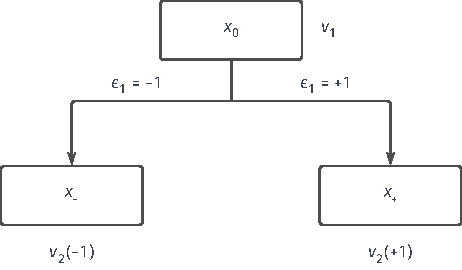
\includegraphics[width=78.281mm]{figures/01-mathematical-preliminaries-upper/02-linear-algebra-and-geometry/tikz/concepts-analysis-functional/query-tree.pdf}
 \functionalinlinefigurecaption{fig:functional-query-tree}
   {两层查询树。根查询$x_0$固定；第一次结果$\epsilon_1=-1$进入左支，第二次查询取$x_-$，结果$\epsilon_1=+1$进入右支，第二次查询取$x_+$。代表树在根处给$v_1$，在两个第二层结点分别给$v_2(-1)$与$v_2(+1)$。评价沿每条分支路径累计均方根误差，因此它不是一个固定两维样本向量，而是随历史变化的查询协议。}
\end{minipage}
\end{center}

\section{本章小结}
\label{sec:functional-summary}

\begin{enumerate}
  \item 把整个函数当作空间元素，必须先明确它是逐点函数还是几乎处处等价类，再选择误差、线性运算和完备性条件。Banach、Hilbert、$L^p$与核空间分别规定不同结构，不能当成彼此排斥的类别；同一底集或相同函数集合也不意味着误差口径相同。

  \item 弱导数通过测试恒等式保留变化信息，Sobolev范数同时控制函数与规定阶导数；它们不自动提供每点或边界读数。读取首先要良定义，随后才判断有界、代表唯一及位置变化；Riesz表示、RKHS和迹各有明确的输入、输出和条件。

  \item 正交展开、积分变换和积分方程分别记录方向、改变函数以及确定未知函数。闭性与完备性保障投影，正交系稠密保障范数展开，紧自伴和Mercer条件保障不同层次的谱结论；压缩迭代还要核对实际自映射和严格常数，不能只凭一个形式核公式取得全部结论。

  \item 函数拟合必须把数据、候选、目标和允许扰动同时给清。表示定理消去数据看不见的方向，具体二次结构才进一步给出有限系统和唯一函数；系数冗余、算法收敛、固定参数的数据稳定以及惩罚参数极限仍按各自变化量判断。积分变分先得到一阶弱条件，具体Poisson与热方程的解理论由后续微分方程章承接。

  \item 有限表示构造、已知函数的能量采样与整个函数类的覆盖数具有不同的近似对象。一个目标存在逼近器不保证找得到参数，能量值一致不保证最优解收敛，容量数量也不直接保证泛化；每一种判断都必须保留其误差、量词和条件。曲面弱微分（\term{Laplace--Beltrami算子}）、球面谱（\term{球谐函数}）、多尺度平滑（\term{尺度空间}）以及跨点搬运所需的几何结构，由流形章继续建立。
\end{enumerate}

